% NOTE(cmo): Once upon a time from below \/ but almost entirely customised with
% very little remaining of original structure.
  % This template was written by John Davies <john.davies@glasgow.ac.uk> 2017-02-06
  % It matches the university specification at the time of writing
  %   for the widths of the page margins and one-and-a-half line spacing
  % You may want to include more packages, particularly for heavy mathematics
  % Please let me know if you find any errors or wish to suggest improvements

% \documentclass[11pt,titlepage,oneside,a4paper]{book}
\documentclass[titlepage,oneside,a4paper,headinclude,
               headheight=16.5pt,footheight=16.5pt,
               chapterprefix,
              %  autoenlargeheadfoot=true,
               parskip=half,
               bibliography=totoc,listof=totoc]{scrbook}
\addtokomafont{disposition}{\rmfamily}
\usepackage{scrlayer-scrpage}
\clearpairofpagestyles
\automark{chapter}
\automark*{section}
\cohead{\rightmark}
\ofoot*{\upshape \thepage}

\usepackage{setspace}
% Set this in the body.
% \setstretch{1.5}
% \onehalfspacing

\usepackage[pdftex]{graphicx}
\usepackage[pdftex]{xcolor}
\graphicspath{{./Figures/}}
% \usepackage{float}
\definecolor{lightGrey}{rgb}{0.9,0.9,0.9}
\definecolor{Red}{rgb}{1.0,0.0,0.0}
% https://personal.sron.nl/~pault/
% Paul Tol's vibrant qualitative colour scheme.
\definecolor{TolBlue}{HTML}{0077BB}
\definecolor{TolCyan}{HTML}{33BBEE}
\definecolor{TolTeal}{HTML}{009988}
\definecolor{TolOrange}{HTML}{EE7733}
\definecolor{TolRed}{HTML}{CC3311}
\definecolor{TolMagenta}{HTML}{EE3377}
\definecolor{TolGrey}{HTML}{BBBBBB}

% NOTE(cmo): See code in PythonTexSetup.tex to generate this.
\definecolor{MplBlue}{rgb}{0.003922,0.450980,0.698039}
\definecolor{MplC0}{rgb}{0.003922,0.450980,0.698039}
\newcommand*{\MplBlueWord}{{\color{MplBlue}blue}}
\newcommand*{\MplBlueWordCap}{{\color{MplBlue}Blue}}
\definecolor{MplOrange}{rgb}{0.870588,0.560784,0.019608}
\definecolor{MplC1}{rgb}{0.870588,0.560784,0.019608}
\newcommand*{\MplOrangeWord}{{\color{MplOrange}orange}}
\newcommand*{\MplOrangeWordCap}{{\color{MplOrange}Orange}}
\definecolor{MplGreen}{rgb}{0.007843,0.619608,0.450980}
\definecolor{MplC2}{rgb}{0.007843,0.619608,0.450980}
\newcommand*{\MplGreenWord}{{\color{MplGreen}green}}
\newcommand*{\MplGreenWordCap}{{\color{MplGreen}Green}}
\definecolor{MplRed}{rgb}{0.835294,0.368627,0.000000}
\definecolor{MplC3}{rgb}{0.835294,0.368627,0.000000}
\newcommand*{\MplRedWord}{{\color{MplRed}red}}
\newcommand*{\MplRedWordCap}{{\color{MplRed}Red}}
\definecolor{MplPurple}{rgb}{0.800000,0.470588,0.737255}
\definecolor{MplC4}{rgb}{0.800000,0.470588,0.737255}
\newcommand*{\MplPurpleWord}{{\color{MplPurple}purple}}
\newcommand*{\MplPurpleWordCap}{{\color{MplPurple}Purple}}
\definecolor{MplBrown}{rgb}{0.792157,0.568627,0.380392}
\definecolor{MplC5}{rgb}{0.792157,0.568627,0.380392}
\newcommand*{\MplBrownWord}{{\color{MplBrown}brown}}
\newcommand*{\MplBrownWordCap}{{\color{MplBrown}Brown}}
\definecolor{MplPink}{rgb}{0.984314,0.686275,0.894118}
\definecolor{MplC6}{rgb}{0.984314,0.686275,0.894118}
\newcommand*{\MplPinkWord}{{\color{MplPink}pink}}
\newcommand*{\MplPinkWordCap}{{\color{MplPink}Pink}}
\definecolor{MplGrey}{rgb}{0.580392,0.580392,0.580392}
\definecolor{MplC7}{rgb}{0.580392,0.580392,0.580392}
\newcommand*{\MplGreyWord}{{\color{MplGrey}grey}}
\newcommand*{\MplGreyWordCap}{{\color{MplGrey}Grey}}
\definecolor{MplYellow}{rgb}{0.925490,0.882353,0.200000}
\definecolor{MplC8}{rgb}{0.925490,0.882353,0.200000}
\newcommand*{\MplYellowWord}{{\color{MplYellow}yellow}}
\newcommand*{\MplYellowWordCap}{{\color{MplYellow}Yellow}}
\definecolor{MplCyan}{rgb}{0.337255,0.705882,0.913725}
\definecolor{MplC9}{rgb}{0.337255,0.705882,0.913725}
\newcommand*{\MplCyanWord}{{\color{MplCyan}cyan}}
\newcommand*{\MplCyanWordCap}{{\color{MplCyan}Cyan}}

\definecolor{UniversityBlue}{HTML}{003865}
\definecolor{SkyBlue}{HTML}{005398}

\renewcommand*{\raggedchapter}{\centering}
\renewcommand*{\chapterformat}{%
\color{SkyBlue}%
\rule{0.3\textwidth}{1pt}%
\hspace{0.5em}%
\scalebox{3}{\thechapter}%
\hspace{0.5em}%
\rule{0.3\textwidth}{1pt}%
\vspace*{-0.5\baselineskip}%
}
\renewcommand*{\sectionformat}{\color{SkyBlue}{\thesection\autodot}\enspace}
\renewcommand*{\subsectionformat}{\color{SkyBlue}{\thesubsection\autodot}\enspace}
\renewcommand*{\subsubsectionformat}{\color{SkyBlue}{\thesubsubsection\autodot}\enspace}

% \usepackage[margin=1em, font=small, labelfont=bf]{caption}
\setcapmargin*{1em}
\setcapindent{1em}
\addtokomafont{caption}{\small}
\addtokomafont{captionlabel}{\bfseries}
% \usepackage{subcaption}
\usepackage{tikz}
\usetikzlibrary{positioning,shapes,fit,arrows,intersections,external,decorations}
\tikzexternalize[prefix=TikzGen/]
\usepackage{pgf}

\usepackage[utf8]{inputenc}
\usepackage[T1]{fontenc}
\usepackage{etoolbox}
% \usepackage{mathpple}
% \usepackage[default,regular,black]{sourceserifpro}
% \usepackage[scaled=0.85]{beramono}
\usepackage{amsfonts,amssymb,amsmath}
\usepackage{bigints}
% \usepackage{fourier}
% \usepackage[charter]{mathdesign}
% \usepackage[notext, nosf, nott]{kpfonts}
\usepackage[default,regular,semibold]{sourceserifpro}
\usepackage[small, T1]{eulervm}
\usepackage[scale=0.8, semibold]{sourcecodepro}
\usepackage{sourcesanspro}
\usepackage{gensymb}
\usepackage[f]{esvect}
% \usepackage[italic]{mathastext}
% \makeatletter

% \DeclareSymbolFont{EulerLetters}{T1}{zeur}{m}{n}
% NOTE(cmo): This will only work with euler but will replace v in math mode with
% \upsilon, which I personally never use. letters symbol font drawn directly
% from euler.sty
% Don't use this one, see below.
% \DeclareMathSymbol{v}{\mathalpha}{letters}{"1D}
% \DeclareMathSymbol{v}{\mathalpha}{letters}{"1D}

% https://tex.stackexchange.com/q/611645/50104
% Thanks to Ulrike Fischer who found a solution that doesn't break urls. But
% shouldn't be necessary now

% \DeclareMathSymbol{\REALV}{\mathalpha}{letters}{`v}
% \DeclareMathSymbol{v}{\mathalpha}{letters}{"0A}
% \makeatletter
% \appto\UrlSpecials{\do\v{\REALV}}
% \makeatother

% Experiments adjusting characters
%%%%%%%%%%%%%%%%%%%%%%%%%%%%%%%%%%%%%%%%%%%%%%%%%%%%%%%%%%%%%%%%%%%%%%%%%%%%%%%%
% \DeclareSymbolFont{SSFLetters}{OT1}{\sfdefault}{m}{n}
% \DeclareSymbolFont{CMletters}{OML}{cmm}{m}{it}
% https://tex.stackexchange.com/a/27536/50104
% \DeclareFontEncoding{FML}{}{}%
% \DeclareFontSubstitution{FML}{futm}{m}{it}%
% \DeclareSymbolFont{fourier}{FML}{futm}{m}{it}
% \DeclareMathSymbol{\nu}{\mathalpha}{fourier}{23}

% \DeclareMathSymbol{v}{\mathalpha}{fourier}{`v}
% % \DeclareMathSymbol{v}{\mathalpha}{SSFLetters}{`v}
% % \DeclareMathSymbol{\nu}{\mathalpha}{CMletters}{23}
% \DeclareMathSymbol{v}{\mathalpha}{CMletters}{`v}
% \makeatother
% \usepackage{concmath}
%%%%%%%%%%%%%%%%%%%%%%%%%%%%%%%%%%%%%%%%%%%%%%%%%%%%%%%%%%%%%%%%%%%%%%%%%%%%%%%%

\usepackage{lipsum}

\renewcommand{\mathbf}{\mathbold} %for Eulervm, uses bold instead of bf
% \let\oldhat\hat
% \renewcommand{\vec}[1]{\vv{#1}} %vec uses esvect
% \renewcommand{\hat}[1]{\oldhat{\mathbf{#1}}}
\DeclareMathOperator{\spn}{span}
\DeclareMathOperator{\row}{row}
\DeclareMathOperator{\cols}{col}
\DeclareMathOperator{\nul}{null}
\DeclareMathOperator{\rank}{rank}
\DeclareMathOperator{\nullity}{nullity}
\DeclareMathOperator{\range}{range}
\DeclareMathOperator{\image}{image}
\DeclareMathOperator{\mathion}{ion}

% upquote fixes quotes in verbatim
\usepackage{upquote}
% microtype for the best microtypographical changes (few end-of-line hypenations :D)
\usepackage{microtype}

% NOTE(cmo): For university specified _print_ margins and headers
% \usepackage[top=1.8cm,bottom=1.8cm,left=4.0cm,
%             right=1.5cm,headheight=15pt,includeheadfoot]{geometry}
% \usepackage{fancyhdr}
% \pagestyle{fancy}
% \fancyhf{}
% \fancyhead[R]{\nouppercase{\rightmark}}
% \fancyfoot[R]{\thepage}
% \renewcommand{\headrulewidth}{0.2pt}
% \newlength{\quarterPage}
% \setlength{\quarterPage}{7.42cm}
\usepackage[toc,page]{appendix}
\usepackage[UKenglish]{babel}
\usepackage{natbib}

\setcitestyle{authoryear,round,semicolon,aysep={}}

% Add extra non-fragile packages here
\usepackage{siunitx}
\sisetup{mode=text}
% Don't indent paragraphs, separate vertically, KOMA can do this.
% \usepackage{parskip}
% The actual magic
\usepackage{pythontex}
% NOTE(cmo): Swap to deptythontex if you need to use the `depythontex' utility
% to see what code has been generated!
% \usepackage[depythontex]{pythontex}

% NOTE(cmo): Set typearea parameters right at the end
% \setstretch{1.5}
\onehalfspacing
% \KOMAoptions{DIV=12, BCOR=11mm}
% \KOMAoptions{DIV=12, BCOR=16mm}
\newlength{\typeareaoffset}
\setlength{\typeareaoffset}{15pt}
\addtolength{\hoffset}{\typeareaoffset}
\KOMAoptions{DIV=12, BCOR=10mm}
% \usepackage{showframe}

\usepackage[draft]{changes}
% \usepackage[final]{changes}

\usepackage{import}
\setpythontexcontext{figurewidth=\the\columnwidth}
\newcommand{\includepgf}[1]{\IfFileExists{#1}{\input{#1}}{}}

\usepackage[pdftex,colorlinks=true,bookmarksnumbered=true,linkcolor=UniversityBlue,
  urlcolor=blue,citecolor=UniversityBlue,bookmarksopen=false,pagebackref=true,
  pdfauthor={},pdftitle={},pdfkeywords={},
  pdfsubject={},pdfcreator={},
  pdfproducer={}, pdfencoding=auto, psdextra, breaklinks=true]{hyperref}

\newcommand*{\Ca}{Ca\,\textsc{ii}}
\newcommand*{\Caii}{Ca\,\textsc{ii}}
\newcommand*{\Caiii}{Ca\,\textsc{iii}}
\newcommand*{\CaLine}{Ca\,\textsc{ii} \SI{854.2}{\nano\m}}
\newcommand*{\Ha}{H$\alpha$}
\newcommand*{\Radyn}{RADYN}
\newcommand*{\Lw}{\textit{Lightweaver}}
\newcommand*{\MsLw}{\textit{MsLightweaver}}
\newcommand*{\Sota}{state-of-the-art}
\newcommand*{\NeedRef}{{\color{Red} REF}}
\newcommand*{\ExpandMe}{{\color{Red} EXPAND}}
\newcommand*{\TODO}[1]{{\color{Red} TODO: #1}}
\newcommand*{\NOTE}[1]{{\color{Red} NOTE: #1}}
\newcommand*{\varv}{\upsilon}
% Roman or math font derivatives
% \newcommand*{\dd}{\mathrm{d}}
\newcommand*{\dd}{d}
\DeclareSIUnit\erg{erg}

\begin{document}
\begin{pythontexcustomcode}{py}
import os
import pickle

import numpy as np
import matplotlib.pyplot as plt
import texfigure
texfigure.preamble_setup()

rc = {
      'axes.titlesize': 12,
      'axes.labelsize': 12,
      'legend.fontsize': 10,
      'xtick.labelsize': 10,
      'ytick.labelsize': 10,
      'xtick.major.pad': 3,
      'xtick.minor.pad': 3,
      'ytick.major.pad': 3,
      'ytick.minor.pad': 3,
      'xtick.direction': 'in',
      'ytick.direction': 'in',
      'savefig.bbox': 'tight'
      }
texfigure.configure_latex_plots(pytex, **rc)
pytex.formatter = texfigure.repr_latex_formatter
\end{pythontexcustomcode}
% NOTE(cmo): This empty block ensures that python tex always "does something"
% and fixes an issue with latexmk looking for the dependencies file
\begin{pycode}
\end{pycode}
\begin{titlepage}
\centering
\vspace*{1cm}  % Need the * or the space is swallowed at the top of the page
\bfseries\Large
Casting a New Light on Radiative Transfer in\\Solar Flare Models:
Synthesis and Inversion\\
\vspace{2cm}
\normalfont\large{\bfseries{
Christopher M. J. Osborne\\
BSc (Hons)\\
}}
\vspace{1.5cm}
Submitted in fulfilment of the requirements for the\\
degree of Doctor of Philosophy\\
\vspace{1.5cm}
Astronomy and Astrophysics Group\\
School of Physics and Astronomy\\
University of Glasgow\\
\vspace{1cm}

\includegraphics[width=0.5\columnwidth]{GlaLogo.pdf}
\\
\vspace{1cm}
% Insert month and year of date deposited with library for final version
September 2021
\end{titlepage}
% Order: https://www.gla.ac.uk/media/Media_549236_smxx.pdf Appendix (from MVLS, also not self-consistent on ordering)
\frontmatter  % Turn off chapter numbering, use roman page numbers
% NOTE(cmo): 1.5 spacing in abstract
% \onehalfspacing
% \setstretch{1.5}
% \KOMAoptions{DIV=last}

\thispagestyle{empty}

\newpage\markboth{}{}

\vspace*{4cm}
\begin{flushright}
\parbox{130mm}{
\hrulefill

This thesis is my own composition except where indicated in
the text. No part of this thesis has been submitted elsewhere for any other degree
or qualification.
\vspace*{1cm}

\textbf{Copyright © ~2021 by Christopher M J Osborne}
\vspace*{0.4cm}

\today

\hrulefill{}}
\end{flushright}

\thispagestyle{empty}
\newpage\markboth{}{}

\vspace*{0.3\textheight}
\begin{center}
\noindent\begin{minipage}{0.8\textwidth}
\emph{I send you this letter on a falling star. Reentry will score and test it but will not melt it away. I write in fire across the sky, a plummet to match your rise.}
\end{minipage}
% \rule{0.8\textwidth}
\end{center}
\noindent\hspace*{0.1\textwidth}\rule{0.8\textwidth}{1pt}\hspace*{0.1\textwidth}
\begin{flushright}
  {This Is How You Lose the Time War\hspace*{0.1\textwidth}}
  \\
  {\small--- Amal El-Mohtar \& Max Gladstone}
\end{flushright}
\chapter{Abstract}

Abstract text goes here.

% NOTE(cmo): 1.0 spacing for table of contents etc
% \singlespacing
% \KOMAoptions{DIV=last}
\tableofcontents
% \listoftables
\listoffigures
% NOTE(cmo): 1.5 spacing in text
% \onehalfspacing
% \setstretch{1.5}
% \KOMAoptions{DIV=last}
\chapter{Preface \& Acknowledgements}

\mainmatter % Turn on chapter numbering, reset page numbers, use arabic
\chapter{Introduction}

\begin{itemize}
    \item The Sun
    \item The Layers of the Sun
    \item The Chromosphere
    \item Flares
\end{itemize}

% ``I'm not lost, because I haven't any idea where to go that I might get lost on the way to. I'd like to get lost, because then I'd know where I was going, you see.''
% -- Catherynne M. Valente, The Girl Who Circumnavigated Fairyland in a Ship of Her Own Making


% ``All you can do, Rosemary – all any of us can do – is work to be something positive instead. That is a choice that every sapient must make every day of their life. The universe is what we make of it. It’s up to you to decide what part you will play.''
% -- Becky Chambers, The Long Way to a Small, Angry Planet
\chapter{Flare Modelling}\label{Chap:FlareModelling}
% spell-checker: disable
%TC:group pycode 0 0
\begin{pycode}[FlareModelling]
name = 'FlareModelling'
chFlareModelling = texfigure.Manager(
    pytex,
    './01aFlareModelling',
    number=1,
    python_dir='./01aFlareModelling/python',
    fig_dir=   './01aFlareModelling/Figs',
    data_dir=  './Data/01aFlareModelling'
)
\end{pycode}
% spell-checker: enable

% \begin{itemize}
%     \item Radiative Transfer Physics
%     \item Hydro and Radiation hydrodynamics
%     \item Numerical approaches to RT and RHD. (combined into the previous sections)
% \end{itemize}

Simulation is a powerful scientific approach that seeks both to validate our understanding of a phenomenon and also learn how it is influenced by various parameters.
Contrary to its dictionary definition, which suggests deceit or merely a surface level resemblance, simulations are essential tools in an astrophysical context.
Astrophysical observations differ greatly from laboratory experiments, due to our lack of knowledge of the configuration and parameters of the system, and inability to repeat particular events.
Simulations therefore represent our best tool for bridging the gap between a theory of the physical processes at work in an observed event, and the observations thereof.
A numerical approach is often needed as the coupled physical processes investigated are typically too complex and non-linear to analytically solve in detail.
There will commonly be free parameters left in these models, some of which can be directly inferred from observation, but others may need to be investigated and later constrained by comparing the model output to observations.
Due to computational or conceptual limitations simplifying assumptions are often required to make these models tractable.

% In the following we will describe the primary physical processes assumed to be at work in solar flares, and how these are modelled, including the primary approximations used.


% \section{Modelling Flares and Observables}

To design a model of solar flares it is first necessary to understand as much as possible from the available observations, so as to ascertain reasonable approximations and the most important processes to include.
By the same, it is necessary to understand which observables vary between flares, to be able to exploit their specific sensitivities and choose those that are sufficiently variable to describe the processes at work and distinguish between flares.
The following builds on many years of work by the solar physics community, and we start from the understanding that has slowly been accrued to present the current state of flare modelling, and an introduction to some of the important numerical theory.
A discussion of the flare observables we are focused on, as well as the techniques used to obtain these is presented in Chap.~\ref{Chap:FlareObservations}.

\section{Radiation Hydrodynamics}

% In our discussion of radiative transfer thus far we have treated the thermodynamic structure of the atmosphere as something constant, however given the short timescales flares evolve over, we know that this is a poor approximation.

It is common to treat flares as a semi-ionised plasma consisting of a single compressible fluid, obeying the equations of hydrodynamics. The influence of the magnetic field can also be included, at which point the equations of magnetohydrodynamics (MHD) are used to describe the motion of the fluid.
Due to the complexity, and resultant numerical difficulties in investigating the widely varying spatial scales that occur in flares (the entire photosphere to coronal region, but requiring a dense sampling of the chromosphere and transition region) with a three-dimensional MHD treatment, it is common to use one-dimensional field-aligned hydrodynamic code.
The assumption here is that the vast majority of observed fluid motions in a flare are along the magnetic field lines, so a single flaring loop can be approximated by a quasi-one-dimensional simulation describing the movement of a fluid through a tube, and the propagation of energy through this medium.
This is due to the strength of the magnetic field, effectively locking the fluid within flux tubes to the field lines.
These are therefore known as field-aligned radiation hydrodynamic codes.

This gas dynamic system can be described by

\begin{equation}
    \begin{aligned}
    \frac{\partial \rho}{\partial t} + \frac{\partial \rho \varv}{\partial z} &= 0\\
    \frac{\partial \rho \varv}{\partial t} + \frac{\partial \rho \varv^2}{\partial z} - \rho g + \frac{\partial P}{\partial z} - \frac{\partial}{\partial z}\left(\mu \frac{\partial \varv}{\partial z}\right) &= 0\\
    \frac{\partial E}{\partial t} + \frac{\partial}{\partial z}\left( E\varv + P\varv - \kappa\frac{\partial T}{\partial z} \right)+ \mu\frac{\partial \varv^2}{\partial z} -\rho \varv g + L - S &= 0,
    \end{aligned}\label{Eq:RhdEquations}
\end{equation}

where $\rho$ is the mass density of the gas, $\varv$ is the bulk velocity, $z$ is the spatial coordinate, $g$ is the local gravitational acceleration, $P$ is the pressure, $\mu$ is the coefficient of dynamic viscosity, $L$ is the radiative loss term, and $S$ is all additional energy source terms, from radiative transfer and atmospheric heating.
In these models the plasma is typically assumed to behave as an ideal gas, and therefore uses the equation of state
$P = n_{\mathrm{tot}} k_B T$, where $n_{\mathrm{tot}}$ is the total particle number density, $k_B$ is Boltzmann's constant, and $T$ is the plasma temperature. Additionally, $\kappa$ is the temperature-dependent coefficient of heat conduction, and is discussed in detail in Sec.~\ref{Sec:NumericalConduction}.

All of the quasi-one dimensional codes solve a variant the RHD equations in \eqref{Eq:RhdEquations}. The first of these describes mass continuity, the second conservation of momentum, and the third conservation of energy.
The nuance typically occurs in ensuring that all terms are solved in a self-consistent fashion and the treatment of the optically thick radiation source and sink terms appearing in the energy equation.

The first generation of hydrodynamic flare models \citet{Nagai1980,Mariska1982,McClymont1983} focused on capturing the gas dynamics of the flaring event, using simplified radiative treatment.
These early models were, in general, much more limited due to computational constraints. \citet{Nagai1980} and \citet{Mariska1982} both employ optically thin losses with ad hoc corrections to avoid over-cooling the lower atmosphere.
\citet{McClymont1983} employ an escape probability formalism for determining the transition rates of hydrogen, which is a faster, less precise method than detailed radiative transfer, but vastly more accurate than assuming the chromosphere to be optically thin (or an ad hoc modulation thereof).
Escape probability methods are unable to directly take radiative backwarming into account -- where radiation produced higher in the atmosphere is absorbed at a lower point -- which can be an important factor for strong solar optical transitions used to diagnose atmospheric properties.

The current generation of RHD codes consists of RADYN \citep{Carlsson1992a,Carlsson1995,Carlsson1999, Allred2015}, FLARIX \citep{Varady2010,Heinzel2015}, and HYDRAD \citep{Bradshaw2003, Bradshaw2013}. RADYN and FLARIX both apply detailed treatment of the radiative losses for certain chromospheric transitions, whilst HYDRAD uses partially precomputed radiative rates for hydrogen (based on the treatment of \citet{Sollum1999}) and radiative losses following the approximations of \citet{Carlsson2012}.
HYDRAD originally focused more on the investigation of non-equilibrium optically thin radiative losses in the corona, and less on the chromosphere, however, recent development has also moved in the direction of an improved chromospheric treatment.
It also differs in its use of a two-fluid model, treating electrons and ions as separate, but coupled, fluids.
In current applications this does not appear to provide significantly different results when applied to flare modelling.

RADYN is derived from the MULTI radiative transfer (RT) code \citep{Scharmer1985, Carlsson1986, Carlsson1992}, and applies the linearisation approach described therein to the entire RHD system, ensuring the self-consistency of all terms. The equations of RHD are solved in an implicit linearised form by Newton-Raphson iteration on the dynamic grid of \citet{Dorfi1987}.
RADYN was originally constructed to investigate the effects of waves propagating through the chromosphere, but was extended by \citet{Abbett1999} to perform some of the earliest simulations of the dynamic flares with detailed radiation treatment in a self-consistent fashion. The code has since been developed further to include improved energy transport treatments, primarily focusing on electron beam energy deposition \citep{Allred2005, Allred2015}.


FLARIX, on the other hand consists primarily of three separate modules. The hydrodynamics is solved by a variant of the NRL Solar Flux Tube Model described in \citet{Mariska1982,Mariska1989}, extended with a MALI module (considering non-overlapping spectral lines with constant background continuum as described in \citet{Rybicki1991}) for detailed radiation transfer, and a test-particle code for determining heating and electron deposition \citep{Varady2010, Heinzel2015}.

RADYN and FLARIX have recently been tested against each other and shown to provide remarkable agreement, despite their different heritage \citep{Kasparova2019}, and early tests also show good consistency with HYDRAD when enabling its recent extensions\footnote{Initial comparisons undertaken following the International Space Science Institute meeting: ``Interrogating Field-Aligned Solar Flare Models: Comparing, Contrasting and Improving'' led by G.S. Kerr and V. Polito.}.

\section{An Eye to the Future: Radiative Magnetohydrodynamics}

Much scientific effort is being invested into the creation of three-dimensional radiative MHD (RMHD) models, which aim to accurately describe all of the physics of a flaring system through the use of large models on supercomputers. The two leading codes are \textit{Bifrost} \citep{Gudiksen2011}, and MURaM \citep{Rempel2009,Rempel2016}. MURaM was originally focused on photospheric magnetoconvection, but has been extended into the corona. It adopts a grey radiative transfer technique that treats all outgoing radiation using a wavelength averaged approach, but has successfully demonstrated the ability to drive self-consistent flare-like eruptions with time-dependent photospheric magnetograms as a boundary condition \citep{Cheung2019}.

\textit{Bifrost} is more focused on a detailed chromospheric treatment; it can apply different combinations of physics modules including multi-group opacities for wavelength dependent radiation transport, the \citet{Sollum1999} model for hydrogen ionisation \citep[following the treatment of][]{Leenaarts2007}, and radiative losses following the method of \citet{Carlsson2012}.
It has been used to investigate solar enhanced networks \citep{Carlsson2016}, the generation of spicules \citep{Martinez-Sykora2017}, and the magnitude of magnetic energy present in the chromosphere \citep{Martinez-Sykora2019}, amongst many other projects.

Currently, neither code can handle the scale of the energy deposition used in the field-aligned flare models, or provide an equivalent chromospheric spatial resolution, but this is an area of very active development.
The field-aligned models remain complementary to these much more complex and computationally intensive models, allowing for more rapid investigation of the relative importance of phenomena to be implemented within the RMHD models, the use wider parameter spaces and higher energy inputs, and easier more compact output that is easier to manipulate and interpret.


\section{Solar Flare Heating}

The aforementioned modern field-aligned RHD codes are primarily designed to simulate the response of a tube of initially quiet solar atmosphere to heating.
This is typically presumed to be due to a beam of energetic electrons precipitating from the corona due to magnetic reconnection.

The direct effects of these electrons must also be considered, as their flux is sufficiently large that their collisions with particles in the lower atmosphere can substantially change the distribution of these particles, exciting and ionising them.
The evolution of the atmosphere will also affect how and where it interacts with these precipitating electrons, coupling an additional problem to the extant RHD system.

There are different methods of solving this problem, the simplest of which is the analytic solution of \citet{Emslie1978} which provides an analytic solution to electron beam energy deposition along the column of plasma under the assumption that all electron energy is lost due to Coulomb collisions with the plasma acting as a cold target.
This is a useful approximate treatment, however terms such as relativistic effects on high energy electrons, return current (heating the corona), and magnetic mirroring are all important here, and ignored in this model. RADYN and FLARIX both include more advanced treatments including these effects; FLARIX uses a test-particle module \citep{Varady2010}, whereas RADYN solves the Fokker-Planck equation \citep[now using the method of ][]{Allred2020}, but both also include the option to use the the simpler analytic Emslie formulation.

Another proposed model for the energy transport and heating in flares is Alfvén heating \citep{Emslie1982, Fletcher2007}, which suggests that energy is transported by Alfvén waves\footnote{These  are transverse waves that propagate along the magnetic field \citep[e.g. ][]{TandbergHanssen1988}.} from the corona to the denser layers at the base of a flaring loop where electrons are locally accelerated.
One argument for this is the so-called ``number problem'' which expresses the difficulty in resupplying the acceleration site in the low density coronal plasma with sufficient electrons to reflect the number observed at their chromospheric impact (this number can be bounded from hard X-ray observations \citep[e.g.][]{Simoes2013}).
The denser regions closer to the electrons' impact location do not suffer from this same scarcity of electrons, and thus represent a possible resolution to this problem.

A simplified variant of this Alfvénic heating model has been investigated by \citet{Kerr2016} inside the \Radyn{} code, and produced notably different spectral line profiles which may agree better with observations than those from an electron beam model.
Further investigation of a more complete implementation of this method and its results are needed.
This approach was also incorporated into HYDRAD by \citet{Reep2016}, which showed the viability of these waves heating the deep chromosphere and triggering explosive chromospheric evaporation.
It is non-trivial to incorporate a full treatment of this phenomenon into RHD codes as it is coupled to the magnetic field, and future improvements are needed to more accurately model these effects and investigate to what extent Alfvénic and electron beam heating occurs simultaneously.

The simulations of flares discussed thus far allow us to model the time-evolution of heating a starting atmosphere and in turn predict line and continuum emission through the tools of radiative transfer.
These detailed results can be compared against observations, and have provided significant insight into chromospheric properties (e.g. \citet{Kuridze2015,RubioDaCosta2016,Kowalski2017,Simoes2017}).
The manual forward-fitting process involved in attempting to reproduce these observations with simulations is both time-consuming and difficult and lies close to the field of automated inversions, which we will address later in Chapters~\ref{Chap:FlareObservations} and \ref{Chap:Radynversion}.

We will now present a more detailed overview of the physics involved in the most important terms of the RHD equations \eqref{Eq:RhdEquations}, starting with complexities of radiative transfer outside of local thermodynamic equilibrium.

\section{Introduction to Radiative Transfer}\label{Sec:IntroRT}

\emph{The content of this section draws primarily from \citet{Hubeny2014} and the paper describing the \Lw{} radiative transfer framework \citep{Osborne2021}.}

Radiative transfer is the science of how radiation propagates through a material: the absorptions, scatterings and emission that happens therein.
Radiation is close to the only conduit through which information can arrive from celestial bodies, and by far the most widely exploited.
It allows us to derive proxies for \emph{in situ} measurements, that cannot otherwise be obtained, due to the distances and extreme conditions being observed.

Everyone is familiar with the concept of images, which show the spatial variation of light but a lot of additional information can be gleaned by analysing radiation in terms of its wavelength variation and polarisation projections.
Using both of these properties is referred to as \emph{spectropolarimetry}, and \emph{spectroscopy} when only the unpolarised intensity is considered.
The most basic property to consider here is the specific intensity, commonly denoted $I(\nu, \vec{d})$ for a particular frequency $\nu$ and direction $\vec{d}$ at a location in space with typical SI units \si{\joule\per\square\metre\per\s\per\hertz\per\steradian}.

A ray propagating through a medium, such as a neutral gas or plasma, will gain a certain amount of energy per unit length due to emission processes, whilst also losing another amount due to absorption and scattering processes. These will depend on the local parameters of the plasma as well as the direction of the ray. For a plasma where the primary interacting species are atomic, we can distinguish bound-bound (spectral lines) and bound-free (continuum) transitions. In the former a bound electron moves between two different sublevels of an atom\footnote{Here "atom" refers to either a neutral atom or an ion}, whilst in the latter the atom either absorbs sufficient energy to free a previously bound electron, or an ion loses sufficient energy to recombine with a free electron.

In addition to the obvious spontaneous emission and absorption processes, there is also a process of stimulated emission which is needed to balance the transitions. This occurs when an electron is stimulated to transition between levels by photons with the same frequency and direction as the photon produced by this transition.

In the following, we will discuss how to obtain the frequency- and direction-dependent outgoing radiation given the emissivity and opacity of the plasma, and how to obtain a self-consistent radiation field and populations for the atomic species outside of the approximations of local thermodynamic equilibrium.

\subsection{The Formal Solution}

For a one-dimensional planar atmosphere the radiative transfer equation (RTE) for the specific intensity along a ray can be written as
\begin{equation}
    \frac{1}{c}\frac{\partial I(\nu, \vec{d})}{\partial t} + \mu \frac{\partial I(\nu, \vec{d})}{\partial z} = \eta(\nu, \vec{d}) - \chi(\nu, \vec{d})I(\nu, \vec{d}),
    \label{Eq:FullTimeDepRte}
\end{equation}
where $\eta$ is the plasma emissivity, $\chi$ is the plasma opacity, $z$ is the spatial coordinate of the stratification of the atmosphere, $t$ represents time, $c$ is the speed of light, and $\mu$ is the cosine of the ray's inclination to the surface normal of the plane-parallel configuration.
We consider that the light crossing time for the propagation of light on a solar scale is small compared to the time-evolution of both the atmosphere and our observations so we ignore the time-derivative term.
Defining the source function $S(\mu, \vec{d}) = \eta(\nu, \vec{d}) / \chi(\nu, \vec{d})$, and the optical depth along a ray from the observer as the number of photon mean free paths along this segment $\tau(z, \nu, \vec{d}) = \int_z^{z_{\mathrm{obs}}} = \chi_\nu(z^\prime) / \mu\, dz^\prime$ we can write the RTE as.
\begin{equation}
    \frac{\partial I(\nu, \vec{d})}{\partial \tau(\nu, \vec{d})} = I(\nu, \vec{d}) - S(\nu, \vec{d}).
    \label{Eq:1DRte}
\end{equation}

Equation \eqref{Eq:1DRte} is a first-order linear differential equation and can be solved with the integrating factor $e^{-\tau(\nu, \vec{d})}$ giving

\begin{equation}
I(\tau_0, \nu, \vec{d}) = I(\tau_1, \nu, \vec{d}) e^{-(\tau_1 - \tau_0)} + \int_{\tau_0}^{\tau_1}S(t_\nu, \nu, \vec{d})e^{-(t_\nu - \tau_0)}\, dt_\nu,
\label{Eq:IntegratedRte}
\end{equation}
for $\tau_0$ the optical depth at the observer and $\tau_1 > \tau_0$ along the line of sight.

The solution in equation \eqref{Eq:IntegratedRte} prescribes nothing about the form of the source function in the atmosphere, and assumes that it varies continuously.
Whilst there are approaches such as Feautrier's \citep{Feautrier1964} that involve casting the problem as a second order differential equation we shall focus on the so-called short-characteristic method consisting of solving the RTE directly between discrete points by prescribing a functional form for its variation between these points. Due to the Feautrier method solving the problem for both an up-going and a down-going ray simultaneously, it cannot handle both Doppler shifts and overlapping lines, and for these reasons we will not discuss it further.

\subsection{Short-Characteristics Methods}\label{Sec:ShortChar}

If a functional form with an analytic integral is chosen for the variation of the source function between defined points then an atmosphere can be treated as a sum of analytic integrals. We shall consider the simplest useful functional form, a linear variation, as an illustrative example.
This approach was first presented by \citet{Olson1987}.

The RTE for one slab of a plane-parallel atmosphere (in the case of outgoing radiation (i.e. $\mu > 0$)) can then be written

\begin{equation}
    I(\tau_0) = I(\tau_1) \exp(- |\tau_0 - \tau_1|) + \int_{\tau_0}^{\tau_1} S(t) \exp(-(t - \tau_0))\, dt.
    \label{Eq:ShortCharForm}
\end{equation}

Now, assuming a linear variation of $S$ with $\tau$ in this slab gives

\begin{equation}
    S(t) = S_{\tau_0} \frac{\tau_1-t}{\tau_1-\tau_0} + S_{\tau_1} \frac{t-\tau_0}{\tau_1-\tau_0},
\end{equation}

where $S_{\tau_i}$ indicates the value of the source function at optical depth $\tau_i$.
This can then be substituted into \eqref{Eq:ShortCharForm} (with $\Delta := \tau_1 - \tau_0$) giving

\begin{equation}
    I(\tau_0) = I(\tau_1) \exp(- |\tau_1 - \tau_0|) +
    \frac{\Delta - 1 + \exp(-\Delta)}{\Delta} S_{\tau_0} +
    \frac{1 - \exp(-\Delta) - \Delta\exp(-\Delta)}{\Delta} S_{\tau_1}.
\end{equation}

In atmospheres with very well resolved spatial grids, this method works quite well, however whenever the true source function has positive curvature, the intensity is overestimated, and underestimated for negative curvature. These effects can become quite significant in more sparsely sampled atmospheres.

The short characteristics method can be improved by using higher order polynomial interpolants, however these can lead to spurious ringing artifacts, negatively affecting their precision. One commonly used robust formulation is the monotonic piecewise parabolic method of \citet{Auer1994}. This method assumes a parabolic variation of the source function across local three point stencils, but limits it to the value obtained from linear interpolation if the parabolic interpolant exits the range bounded by these three points.

Other interpolating functions can be used. For example, the cubic Bézier spline interpolant of \citet{DelaCruzRodriguez2013}, provides a higher order approximation in regions of smooth variation, and can be limited through the control points to prevent any ringing instability. A similar approach has been taken with the BESSER quadratic Bézier spline approach of \citet{Stepan2013}.
All of these methods can be derived analogously to the linear formal solver presented above.

\subsection{Other Formal Solvers}

\citet{Janett2018} proposes a novel approach to the formal solver,  using an optimised solver for the differing optical thickness in each slab. They show that this leads to substantial performance benefits whilst also being more numerically stable. They comment that whilst higher order formal solvers will theoretically converge better to the true result, due to the assumptions that are made in their derivation, this will only occur if the variation of the source function in relevant regions of the atmosphere is sufficiently smooth. The modern 3D RMHD simulations use relatively coarse spatial grids with large transients in atmospheric parameters that risk provoking instability in the higher order formal solvers, especially in the case of full Stokes radiative transfer.
As work continues on these higher resolution RMHD simulations an investigation into how each formal solver handles discontinuous parameters is needed.
An accurate treatment of steep gradients and discontinuities is not just valuable to the RMHD models, but important to all radiative transfer modelling, as a reduction in the spatial resolution needed to correctly evaluate radiative transfer can lead to significant reductions in computational requirements, making more complex simulations possible.


\subsection{LTE vs NLTE}

With the understanding of how to design and implement formal solvers for the radiative transfer equation, we have the ability to compute the radiation leaving an atmosphere from the opacity and emissivity structure.
The values of these depend on the atomic populations, and their distribution across energy levels and ionisation states.

As stars like the Sun radiate energy into the cosmos, it is clear that they cannot be in total thermal equilibrium.
However, it is reasonable to suggest that if the atmosphere is sufficiently collisional then a form of local thermodynamic equilibrium (LTE) holds, whereby local parcels of the plasma are effectively in thermodynamic equilibrium such that Kirchhoff's laws of radiation hold.
When a species within a plasma is in LTE its population distribution can be computed using the Saha-Boltzmann equation.
This is the case for spectral lines that form in the photosphere, and the associated level populations, emissivity, and opacity can all be computed directly from local thermodynamic quantities\footnote{If the electron density is not known \textit{a priori} then an iteration scheme using the Saha-Boltzmann equation is necessary to determine consistent values of both the electron density and the atomic populations.}.

If the radiative rates instead dominate the total transitional rates for the species then the particle distribution can no longer be governed by purely local parameters and we enter the realm of non-LTE (NLTE) physics.
This occurs as we enter the chromosphere, where the collisional rates decrease, and the radiation field couples the atomic populations in different regions together.
The core focus of NLTE radiative transfer is to determine atomic populations consistent with the local thermodynamic parameters of the atmosphere and the non-local radiation field.
Until otherwise specified, we will consider that the electron density throughout the atmosphere is known and consider it part of the atmospheric model.

Expressing this mathematically, we write the total transition rate $P_{ij}$ between levels $i$ and $j$ (with the convention that $i < j$) as
\begin{equation}
    P_{ij} = R_{ij} + C_{ij},
\end{equation}
where $R_{ij}$ is the rate of radiative transitions (due to absorption, spontaneous, and stimulated emission) and $C_{ij}$ is the rate of collisional transitions.
As the total population of each element must remain constant we can write the kinetic equilibrium equation (which can be derived from the Boltzmann equation)
\begin{equation}
    \frac{\partial n_l}{\partial t} + \nabla \cdot (n_l \vec{\varv}) = \sum_{l^\prime\neq l} (n_{l^\prime} P_{l^\prime l}) - n_l \sum_{l^\prime\neq l} P_{ll^\prime},
    \label{Eq:KinEq}
\end{equation}
where $n_l$ is the number density of level $l$ of the atomic species in question.

Equation \eqref{Eq:KinEq} is frequently simplified to the statistical equilibrium equation, by setting the left-hand side to 0 giving
\begin{equation}
\sum_{l^\prime\neq l} (n_{l^\prime} P_{l^\prime l}) - n_l \sum_{l^\prime\neq l} P_{ll^\prime} = 0.
\label{Eq:StatEq}
\end{equation}
In Chaps.~\ref{Chap:TimeDepRt} and \ref{Chap:2DRT} we will discuss when the full time-dependent solution need be considered over the simpler statistical equilibrium solution.
The former of these requires a history of the atomic populations in the atmosphere, typically from a time-evolving model such as an RHD simulation, whereas the latter associates a unique solution of atomic populations to a given atmosphere.\footnote{The uniqueness of the solution was proven by \citet{Rybicki1997} for the linear case presented here. I have found no equivalent proof for the non-linear system when a variable electron density is also considered.}
In the following, even when considering the time-dependent problem, we assume that the timescale over which each step in our numerical simulation is integrated is long compared to the light-crossing time for the regions where each transition is optically thick.
If this is not the case, then a different formulation of the formal solver will be required, so as to solve \eqref{Eq:FullTimeDepRte}.

\subsection{Collisional Rates}

There are many collisional processes by which electrons can transition between energy levels in a plasma, including ionisation and recombination processes.
These include excitation of ions by electrons, ionisation and excitation of neutral by electrons, excitation by protons and neutral hydrogen, as well as charge exchange with these species.
There are more advanced formulations that depend on complex functional forms derived from laboratory work and theoretical analysis, such as those of \citet{Burgess1983, Arnaud1985}.

In most cases, the collisional rates are assumed to only depend on local plasma properties, such as the temperature, total particle density, and electron density, with the particles locally following Maxwellian velocity distributions that connect the upwards and downwards collisional rates for a process through detailed balance i.e., $n_i^* C_{ij} = n_j^* C_{ji}$, where $n_i^*$ indicates the LTE population of level $i$.
This is not the case for non-thermal rates, such as those of \citet{1993Fang} which consider collisional excitation by non-thermal electrons from the electron beams used in RHD simulations, but are still computed from local parameters.

\subsection{Emissivity and Opacity}

To mathematically formulate the radiative rates that are so important to $P_{ij}$ in a NLTE context we must first formulate expressions for emissivity and opacity.
There are two forms of transition we need to consider for atomic radiative transfer, spectral lines, and continua.
In spectral lines, the three processes that need to be understood to develop a model for emissivity and opacity are spontaneous and stimulated emission, and absorption.
The magnitude of these terms are controlled by the Einstein coefficients $A_{ji}$, $B_{ij}$, and $B_{ji}$ respectively, which are related by the Einstein relations.

Spectral lines have a rest frequency $\nu_{ij}$  defined by
\begin{equation}
    \nu_{ij} = \frac{h}{\Delta E_{ji}},
\end{equation}
where $h$ is Planck's constant and $\Delta E_{ji}$ is the energy difference between levels $j$ and $i$.
Bound-bound transitions between states in a static plasma are not infinitely fine, but are instead broadened by a number of factors such as natural broadening from uncertainty in the lifetime of the upper state, Doppler broadening due to random thermal motions in the plasma, and collisional broadening (e.g. van der Waals, and Stark broadening\footnote{van der Waals broadening is due to an interaction between an excited atom and the dipole it induces over a neutral atom, whilst Stark broadening is due to the interaction between an atom and a charged particle.} %(linear Stark effect for hydrogen and quadratic for all species following the Weisskopf approximation of impact theory).}). N.B. Quadratic typically << 0.1x linear for H.
The net effects of these processes typically leads to spectral line profiles being modelled as a Voigt function (the convolution of Gaussians and Lorentzians).
The Gaussian terms are due to Doppler broadening, whilst the other terms are typically modelled as Lorentzians, although more accurate treatments of Stark broadening such as those employed \citet{Kowalski2017} are non-Lorentzian, and must be separately convolved with the Voigt profile produced from the previous terms.
The normalised line absorption profile then describes the probability of a photon with a certain energy being absorbed by the transition.

Typically it is assumed that the plasma is sufficiently collisional for elastic collisions to redistribute the electrons of an atom in an excited state over all sub-states of an energy level prior to emission.
If this is not the case then the frequency of the outgoing photon will be correlated with the frequency of the photon that excited the atom into this state.
Thus the spectral line will have an emission profile distinct from its absorption profile.
This effect is known as partial redistribution (PRD) and will be discussed in Sec.~\ref{Sec:Prd}.
The typical state of affairs, where there is sufficient redistribution from elastic collisions for these two processes to be uncorrelated is known as complete redistribution (CRD).
In the following, we will always express line emission processes through an emission profile for generality, even if they are treated as CRD.

Continua, or bound-free transitions, depend instead on photoionisation cross-sections.
In the case of hydrogenic ions these fall off with $1/\nu^3$ (for photons of frequency $\nu$) as the energy of the ionising photon increases away from the continuum edge.
The edge of a continuum is defined by the ionisation potential for an atom in the bound-state of this transition, as only photons with an energy equal to or greater than this are capable of photoionising the element.
In general these cross-sections and their variations are determined from laboratory experiments and numerical solutions of the Schr\"{o}dinger equation.
The photoionisation cross-section describes how likely the atom is to interact with a photon of a particular energy through this bound-free transition.
Its partner processes (like spontaneous and stimulated emission for bound-bound transitions) are spontaneous and stimulated recombination, whereby an electron is captured by the atom and a photon is released with energy equal to the excess energy of the system.
These are related to the photoionisation cross-section and the local plasma parameters by the Milne relations.

There are also free-free interactions between particles (often known as \emph{bremsstrahlung}), where electrons and ions interact, and the electron gains or loses energy through absorption or emission of a photon.
This process also has a characteristic cross-section and is considered as part of the background opacities and emissivities.

Following the notation of \citet{Rybicki1992} and \citet{Uitenbroek2001} the emissivity $\eta$ and opacity $\chi$ for a transition can then written
\begin{align}
    \label{Eq:Emis}
    \eta_{ij} &= n_j U_{ji}(\nu, \vec{d}), \\
    \label{Eq:Opac}
    \chi_{ij} &= n_i V_{ij}(\nu, \vec{d}) - n_j V_{ji}(\nu, \vec{d}).
\end{align}
The $U$ and $V$ terms are defined for bound-bound and bound-free transitions as
\newlength{\WidestCase}
\settowidth{\WidestCase}{$n_e\Phi_{ij}(T)\left(\frac{2h\nu^3}{c^2}\right)e^{-h\nu/k_B T}\alpha_{ij}(\nu),$}
\begin{align}
    \label{Eq:Uji}
    U_{ji} =&
    \begin{cases}
        \frac{h\nu}{4\pi}A_{ji}\psi_{ij}(\nu, \vec{d}), & \textrm{bound-bound} \\
        n_e\Phi_{ij}(T)\left(\frac{2h\nu^3}{c^2}\right)e^{-h\nu/k_B T}\alpha_{ij}(\nu), & \textrm{bound-free},
    \end{cases}\\
%
    \label{Eq:Vij}
    V_{ij} =&
    \begin{cases}
        \makebox[\WidestCase][l]{$\frac{h\nu}{4\pi}B_{ij}\phi_{ij}(\nu, \vec{d}),$} & \textrm{bound-bound} \\
        n_e\Phi_{ij}(T)e^{-h\nu/k_B T}\alpha_{ij}(\nu), & \textrm{bound-free},
    \end{cases}\\
%
    \label{Eq:Vji}
    V_{ji} =&
    \begin{cases}
        \makebox[\WidestCase][l]{$\frac{h\nu}{4\pi}B_{ji}\psi_{ij}(\nu, \vec{d}),$} & \textrm{bound-bound} \\
        \alpha_{ij}(\nu), & \textrm{bound-free},
    \end{cases}
\end{align}
where $\phi$ is the line absorption profile, $\psi$ is the line emission profile, $\alpha_{ij}$ is the photoionisation cross-section, $n_e$ is the local electron density, and $k_B$ is the Boltzmann constant.
$\Phi$ is the Saha-Boltzmann equation defined by
\begin{equation}
    n_e\Phi_{ij}(T) = \frac{n^*_i}{n^*_j} = \frac{g_i}{2g_j}\left( \frac{h^2}
    {2\pi m_e k_B T} \right)^{3/2} \exp{\left(  \frac{\Delta E_{ji}}{k_B T}\right)},
\end{equation}
where $n^*$ is the population of the species in LTE, $m_e$ is the electron mass, $\Delta E_{ji}$ is the energy difference between levels $j$ and $i$, and $g_i$ is the statistical weight of level $i$.
By convention we define $U_{ij} = U_{ii} = V_{ii} = 0$ and $\chi_{ij} = -\chi_{ji}$.
From these definitions we see that the $U$ quantities relate to spontaneous emission, whereas the $V$ quantities describe stimulated processes.
In the case of complete redistribution, where $\psi = \phi$, all of the $U$ and $V$ terms are constant at each location in a given atmosphere, and the variation in emissivity and opacity depends on the atomic populations.

\subsection{Radiative Rates}

The radiative rates that are needed to solve the kinetic or statistical equilibrium equations are an expression of the number of upward ($ij$) and downward ($ji$) transitions due to absorption, spontaneous and stimulated emission processes (and the equivalent bound-free processes).
The formulation of emissivity and opacity through $U$ and $V$ also allows us to express the radiative rates succinctly for both upwards and downwards transitions in lines and continua at each location in the atmosphere as
\begin{equation}
    \label{Eq:RadiativeRates}
    R_{ll^\prime} = \oint \int \frac{1}{h\nu} \left( U_{ll^\prime}(\nu, \vec{d}) + V_{ll^\prime}(\nu, \vec{d})I(\nu, \vec{d}) \right)\,d\nu\,d\Omega,
\end{equation}
where $I(\nu, \vec{d})$ is the specific intensity at this location for a given frequency $\nu$ and direction $\vec{d}$.
It is through $I$ that the non-locality of the radiation field enters the problem.

\subsection{General Source Function}

Where multiple atomic species are present, the total emissivity and opacity are simply the sum of the emissivity and opacity for every transition on each atom at the current frequency and direction. It is common to additionally consider scattering by processes such as Thomson scattering, in which case the source function will be written
\begin{equation}
    S(\nu, \vec{d}) = \frac{\eta_\mathrm{tot}(\nu, \vec{d}) + \sigma(\nu)J(\nu)}{\chi_\mathrm{tot}(\nu, \vec{d})},
\end{equation}
where the ``tot'' subscript refers to these terms being summed over all interacting species, $\sigma$ describes the frequency-dependent coherent and isotropic continuum scattering cross-section, and
\begin{equation}
    J(\nu) = \frac{1}{4\pi}\oint I(\nu, \vec{d})\, d\Omega
\end{equation}
% NOTE(cmo): This angle-average term is what is computed directly from the sum_updown sum_i 0.5 * wmu_i * I, i.e., the averaging is rolled in when we use the integration. The 1/4pi vanishes due to normalisation and the fact we're in ``mu-space''. The 4pi terms all come back in wlambda, but check setup_wavelength on the _atom_ for this, it's not super clear.
is the angle-averaged intensity at frequency $\nu$.

\subsection{Iterative Solutions}

Now we have an expression for the radiative rates in each transition that can be computed numerically given the local value of the intensity, however the radiation field is not known \textit{a priori}.
Clearly, an iterative scheme will be needed to find a stable set of populations yielding a self-consistent radiation field.

If we treat the formal solver as an operator $\Lambda$ yielding the intensity from the source function throughout the atmosphere, i.e.
\begin{equation}
    I(\nu, \vec{d}) = \Lambda_{\nu,\vec{d}}[S(\nu, \vec{d})],
    \label{Eq:LambdaOperator}
\end{equation}
then starting from an initial estimate of the atomic populations (e.g. LTE) we can compute the radiation field throughout the atmosphere and iteratively use this to update the populations by solving \eqref{Eq:KinEq}. This is known as Lambda iteration (after the operator used) and presents woefully poor convergence in optically thick conditions as the size of the population updates stagnate long before the true NLTE populations are obtained.

The failure of Lambda iteration can be remedied by a process known as operator splitting, first introduced by \citet{Cannon1973} whereby we set
\begin{equation}
    \Lambda = \Lambda^* + (\Lambda - \Lambda^*),
\end{equation}
with $\Lambda^*$ an approximation of $\Lambda$. The iterative scheme them becomes
\begin{equation}
    I(\nu, \vec{d}) = \Lambda_{\nu, \vec{d}}^*[S(\nu, \vec{d})] + (\Lambda_{\nu, \vec{d}} - \Lambda_{\nu, \vec{d}}^*)[S^{\dagger}(\nu, \vec{d})],
    \label{Eq:Ali}
\end{equation}
where $\dagger$ identifies values from the previous iteration. This method is termed accelerated Lambda iteration (ALI), and can be shown to accelerate convergence by significantly amplifying the size of the corrections that would be computed by Lambda iteration at large optical depths, for an appropriately chosen $\Lambda^*$.
From \eqref{Eq:Ali} we can see that it is necessary to invert $\Lambda^*$ to obtain the updated value of $S$, on which $I$ is also dependent.
For a two-level atom this is discussed at length in Chaps 12 and 13 of \citet{Hubeny2014}.
The full coupling of the terms in the multilevel NLTE problem will be made explicit in Sec.~\ref{Sec:MALI} when the MALI methods are presented; for now it is clear that the source function depends on the emissivity and opacity of each species, which in turn are controlled by the atomic populations, which are affected by the local radiation field.

A good choice for $\Lambda^*$ is not immediately evident, as it should be cheap to construct and invert, whilst providing a good approximation of $\Lambda$.
\citet{Scharmer1981} presented an upper triangular approximate operator that fits these criteria and showed its relation to the core-saturation approach of \citet{Rybicki1972} (where the net rates in the line core and wing are treated separately to precondition the net radiative rates by removing the large proportion of photons that are emitted in the wing and immediately reabsorbed).

\citet{Olson1986} proposed the use of the diagonal of the true $\Lambda$ operator as an approximate operator, and showed that this is close to optimal, and is clearly trivial to invert (as it is a scalar at each location in the atmosphere).
Now, the diagonal of $\Lambda$ is easy to obtain by setting a test source function $\mathcal{S}=\delta_{dd^\prime}$ (where $\delta$ is the Kronecker delta) and computing
\begin{equation}
    \Lambda^* = \Lambda[\mathcal{S}].
\end{equation}
Taking the example of the linear short characteristic formal solver presented in Sec.~\ref{Sec:ShortChar} and substituting this definition of $\mathcal{S}$ we obtain
\begin{equation}
    \Lambda^*_{\nu, \vec{d}} = \frac{\Delta - 1 + \exp(-\Delta)}{\Delta},
\end{equation}
where $\Delta$ is defined as in Sec.~\ref{Sec:ShortChar}.
The approximate operator can be computed analogously for other formal solvers.

\subsection{Solving the multilevel NLTE problem}\label{Sec:MALI}

Starting from the radiative transfer equation \eqref{Eq:1DRte} and the kinetic equilibrium equation \eqref{Eq:KinEq} we can construct a framework with which to solve the multilevel NLTE problem.
The primary term of interest is the right-hand side of \eqref{Eq:KinEq}, which is concerned with the atomic transition rates.
This is also shared with the statistical equilibrium equations \eqref{Eq:StatEq}, and thus we will solve the latter of these and return to the former later.
We follow the approach of \citet{Rybicki1992} and \citet{Uitenbroek2001}, which is known as Multi-level Accelerated Lambda Iteration (MALI) with full-preconditioning.
The full-preconditioning approach handles arbitrary overlaps of lines and continua for multiple multilevel atoms.
Earlier MALI methods \citep{Rybicki1991} are capable of handling lines overlying a constant background continuum, but not interacting with each other.
These methods describe a form of radiative transfer that is still based on a transition by transition description of the problem.
\citet{SocasNavarro1997} proved that this approach can be numerically equivalent to the linearised ALI method of \citet{Scharmer1985} implemented in the MULTI code \citep{Carlsson1986,Carlsson1992} provided the same assumptions are made in the design of the local operator.
Note that we distinguish between the linearised ALI method and the older method of complete linearisation \citep[e.g. ][]{Auer1969, Auer1973, Auer1976}.
The latter of these is significantly more computationally demanding and less numerically stable than the ALI based methods we are considering here \citep[a comparison of MULTI and LINEAR-B is shown in][]{Carlsson1986}.

As MALI with full-preconditioning directly supports all forms of overlapping transitions and the interactions between them whilst retaining the convergence properties of the ALI method, we focus solely on this method in the following description of radiative transfer and inclusion in the \Lw{} framework.
Whilst there are also more rapidly converging methods (which can be viewed as extensions and variants of the ALI approach) such as the Gauss-Seidel and successive-over-relaxation methods of \citet{TrujilloBueno1995} (with the extension to multilevel systems presented by \citet{Paletou2007}), the forth-and-back implicit Lambda iteration of \citet{AtanackovicVukmanovic1997} (extended to multilevel systems by \citet{Kuzmanovska2017}), and even the multi-grid method of \citet{FabianiBendicho1997}, we opt for this well-tested method that is proven stable and reliable in a wide variety of situations.
This is particularly key when considering modelling of flares, which present much larger variations in parameters and steeper gradients than the quiet Sun models or academic semi-empirical models often considered.
The other, more rapidly convergent, methods present possible avenues of improvement for \Lw{} in the future.

Now, following \citet{Rybicki1992} and \citet{Uitenbroek2001} and substituting \eqref{Eq:LambdaOperator} into \eqref{Eq:StatEq}, and subsequently expanding the radiative rates gives
\begin{equation}
\begin{aligned}
   \sum_{l^\prime\neq l} &(n_{l^\prime}C_{l^\prime l}) +
   \sum_{l^\prime\neq l} \oint \int \frac{1}{h\nu} n_{l^\prime} (U^\dagger_{l^\prime l} + V^\dagger_{l^\prime l} I(\nu, \vec{d}))\, d\nu\, d\Omega\\
   -
   n_l &\sum_{l^\prime\neq l} C_{l l^\prime} -
   n_l \sum_{l^\prime\neq l} \oint \int \frac{1}{h\nu} (U^\dagger_{l l^\prime} + V^\dagger_{l l^\prime} I(\nu, \vec{d}))\, d\nu\, d\Omega
   = 0.
   \label{Eq:StatEqExpanded}
\end{aligned}
\end{equation}
$U$ and $V$ are marked with daggers so as to later incorporate the necessary PRD effects.
\citet{Rybicki1992} defined a new operator $\Psi$ such that
\begin{equation}
    \Psi_{\nu, \vec{d}}[y] = \Lambda_{\nu, \vec{d}}[(\chi^\dagger)^{-1}y]
\end{equation}
These two operators are equivalent for a converged solution as $\chi^\dagger = \chi$, but the use of this operator is necessary to obtain the form of statistical equilibrium equations preconditioned to be linear in the atomic populations that is core to this method.

The operator splitting technique is again applied here. We then have
\begin{equation}
    I(\nu, \vec{d}) = \Psi^*[\eta(\nu, \vec{d})] + (\Psi - \Psi^*)[\eta^\dagger(\nu, \vec{d})],
\end{equation}
and then considering the effects on one atom, under the assumption that background emissivity and opacity do not change during an iteration
\begin{equation}
    I(\nu, \vec{d}) = I^\dagger(\nu, \vec{d})
                    - \sum_j\sum_{i<j}\Psi^*[n^\dagger_j U^\dagger_{ji}]
                    + \sum_j\sum_{i<j}\Psi^*[n_j U^\dagger_{ji}],
\end{equation}
where $i$ and $j$ refer to the levels present in the atomic model.

The first two terms of this expression are often termed $I^\mathrm{eff}$ and in the case of a diagonal $\Psi^*$ operator this represents the non-local contribution to the radiation field from the current atom, and the contribution from all other species.

We can write \eqref{Eq:StatEqExpanded} as
\begin{equation}
    \Gamma \vec{n} = \vec{0},
    \label{Eq:StatEqMatVec}
\end{equation}
where $\Gamma$ is a matrix consisting of the sum of $\Gamma^R$ due to the radiative contributions, and $\Gamma^C$ from the collisional contributions. $\vec{n}$ is the vector of the updated level populations for the species at this point in the atmosphere.
We can then write
\begin{align}
\begin{split}\label{Eq:GammaR}
    \Gamma^R_{ll^\prime} = \oint \int \frac{1}{h\nu} \bigg( U^\dagger_{l^\prime l} + V^\dagger_{l^\prime l}I_{\nu, \vec{d}}^\mathrm{eff} -
    \left(\sum_{m\neq l}\chi^\dagger_{lm}\right) \Psi^*_{\nu, \vec{d}} \left[ \sum_p U^\dagger_{l^\prime p} \right] \bigg)\, d\nu\,d\Omega
\end{split}
\end{align}
for $l\neq l^\prime$.
The problem is now represented by a system of equations linear in the level populations.
Due to the necessity of total number conservation the sum of the entries in each column of $\Gamma$ must be 0, which allows us to compute the diagonal terms as
\begin{equation}
    \Gamma_{ll} = -\sum_{m\neq l} \Gamma_{ml}.
\end{equation}

An additional constraint must be applied to \eqref{Eq:StatEqMatVec} to determine the new populations, to avoid the trivial solution of $\vec{n} = \vec{0}$, which is otherwise always a valid solution.
This constraint is typically expressed through local population conservation, which amounts to replacing one of the rows of $\Gamma$ with ones, and the associated entry in the right-hand-side zero-vector with the local species number density $n_\mathrm{total}$.
There is then a $\Gamma$ matrix at each point in the atmosphere for each atomic species being considered in detail; each of these is square with dimension equal to the number of levels in the atomic model for this species.
This system can then be solved for $\vec{n}$, independently at each location in the atmosphere, as the current estimate of non-local coupling through the radiation field is already present in the terms that compose $\Gamma$.

Iterating the populations through \eqref{Eq:StatEqMatVec} with interleaved formal solutions gives us a reliable and rapidly converging method for solving the multilevel NLTE problem with multiple atoms and overlapping transitions as used in the \Lw{} framework.
A more detailed description of the numerical implementation is provided in the \Lw{} paper \citep{Osborne2021}.

\subsection{Time-Dependent Population Updates}\label{Sec:TimeDepPopUpdates}

As discussed previously, an iterative update to the populations in the statistical equilibrium case can be phrased as $\Gamma \vec{n} = \vec{0}$.
A variant of this method can also be applied to the time-dependent form of the kinetic equilibrium equations \eqref{Eq:KinEq}.
We will not directly treat the advection term of equation \eqref{Eq:KinEq}, as this requires consideration of hydrodynamic effects and the discretisation schemes used therein (due to the large gradients of these populations that occur in the solar atmosphere)\footnote{An overview of the methods used to numerically solve the conservation laws of hydrodynamics is provided in Sec.~\ref{Sec:IntroConsLaws}.}.
We can, however, discretise $\partial n / \partial t = \Gamma \vec{n}$ as
\begin{equation}
    \label{Eq:ThetaDisc}
    \frac{\vec{n}^{t+1} - \vec{n}^t}{\Delta t} = \theta \Gamma^{t+1} \vec{n}^{t+1} + (1-\theta)\Gamma^{t} \vec{n}^{t},
\end{equation}
where $\theta$ indicates the degree of implicitness, the $t$ and $t+1$ indices indicate the start and end of the timestep being integrated respectively, and $\Delta t$ the duration of the timestep.
$\vec{n}^{t+1}$ can then be found by rewriting \eqref{Eq:ThetaDisc} as
\begin{equation}
    \label{Eq:TimeDepSystem}
    (\mathbb{I} - \theta\Delta t \Gamma^{t+1}) \vec{n}^{t+1} = (1-\theta)\Delta t \Gamma^{t}\vec{n}^{t} + \vec{n}^{t},
\end{equation}
with $\mathbb{I}$ the identity matrix.
This system is then iterated until $\vec{n}^{t+1}$ converges, for a new evaluation of $\Gamma^{t+1}$ at each iterate.
This is known as a theta-method, and whilst semi-implicit schemes are possible by setting $0 < \theta < 1$, we have not found these necessary, and adopt the fully implicit $\theta=1$ in \Lw{}.

\subsection{Partial Frequency Redistribution}\label{Sec:Prd}

Most solar spectral lines form in regions where complete frequency redistribution (CRD) holds.
That is to say that the plasma is sufficiently collisional that elastic collisions redistribute electrons across all sub-states of an energy level prior to emission.
In this case, the emission frequency of a photon is not correlated with the frequency of the photon absorbed to excite the atom into this state i.e. photons are completely redistributed in frequency and the line emission and absorption profiles are equal.
In lower density regions with strong, typically resonance\footnote{A transition whose lower state is the ground state of the atom is known as a resonance transition.}, lines where radiative effects dominate over collisional effects, there is said to be a natural population of a certain level: a population where the emission frequency is correlated to the absorption frequency, and has not been redistributed by collisions \citep{Hubeny2014}.
The line's emission and absorption profiles then differ and this coherent scattering must be treated explicitly.
This imposes substantial computational effort, but we will briefly describe the key points of the process, and how it fits into the MALI framework following \citet{Uitenbroek2001} and \citet{Hubeny2014}.

We can define the emission profile coefficient $\rho_{ij} = \psi_{ij} / \phi_{ij}$, at which point all $U$ and $V$ terms can be rewritten in terms of $\rho_{ij}$ and $\phi$, and $\dagger$ on these terms refers to the value of $\rho_{ij}$ evaluated at the previous iterate (analogous to $n^\dagger$).

From this definition of $\rho_{ij}$, under the assumptions of a line with an infinitely sharp lower level and broadened upper level, and the validity of PRD being in the atomic frame being approximated by PRD in the observer's frame \citep{Uitenbroek2001}, following \citet{Hubeny2014} we have
\begin{align}
\begin{split}
    \rho_{ij}(\nu, \vec{d}) = 1 + &\gamma\frac{\sum_{l < j}n_j B_{lj}}{n_j P_j} \oint\frac{1}{4\pi}\int I(\nu^\prime, \vec{d}^\prime) \\ &\cdot \left[ \frac{R^{II}_{lji}(\nu^\prime, \vec{d}^\prime; \nu, \vec{d})}{\phi_{ij}(\nu, \vec{d})} - \phi_{lj}(\nu^\prime, \vec{d}) \right]\,d\nu^\prime\,d\Omega^\prime,
\end{split}
\end{align}
where $R^{II}$ is the generalised redistribution function for transitions of this kind \citep{Hubeny1982}, and $\gamma$ is the coherency fraction.
The $lji$ subscript on $R^{II}$ describes the scattering process, indicating that electrons can start from any level in the range $[i, j)$.
These scattering processes are then summed.
The cross-redistribution, or Raman scattering, processes for which $l\neq i$ are typically less important than resonance scattering ($l = i$).
Only considering the latter of these simplifies the evaluation $\rho_{ij}$.
The redistribution function describes the probability that a photon with frequency $\nu^\prime$ and direction $\vec{d}^\prime$ is re-emitted with frequency $\nu$ and direction $\vec{d}$.

The coherency fraction $\gamma$ describes the probability of a photon being emitted from its current sublevel of the energy level $j$, prior to an elastic collision that would redistribute it across the sublevels of $j$.
This is computed as
\begin{equation}
    \gamma = \frac{P_j}{P_j + Q_j},
\end{equation}
where $P_j$ is the total depopulation rate of level $j$, and $Q_j$ is the total rate of elastic collisions affecting this level.

Ignoring bulk plasma motions that create anisotropy in the radiation field, the integrals over angle and frequency can be split, and render the calculation of this angle-averaged form of $\rho_{ij}$ much simpler and less computationally demanding.
Also defining $g_{II}(\nu, \nu^\prime) = R^{II}(\nu, \nu^\prime)/\phi_{ij}(\nu^\prime)$ such that the fast approximation of \citet{Gouttebroze1986} and \citet{Uitenbroek1989} can be employed, and ignoring cross redistribution terms we have
\begin{equation}
    \label{Eq:RhoPrdAa}
    \rho_{ij}(\nu) = 1 + \gamma \frac{n_i B_{ij}}{n_j P_j} \left( \int g_{II}(\nu, \nu^\prime) J(\nu^\prime)\,d\nu^\prime - \bar{J}_{ij} \right),
\end{equation}
where
\begin{equation}
\bar{J}_{ij} = \frac{1}{4\pi} \oint \int I(\nu, \vec{d}) \phi(\nu, \vec{d})\,d\nu\,d\Omega = \frac{R_{ij}}{B_{ij}}
\end{equation}
is the frequency-integrated mean intensity across the transition.
In the case of plasma flows we adopt the approximate hybrid treatment of \citet{Leenaarts2012}, using $J$ in the plasma's rest frame, to compute $\rho_{ij}$ in this same frame.
Its value is then interpolated to find the value of $\rho_{ij}$ at the Doppler shifted value in the observer's frame.
The additional computational cost of this hybrid method over the angle-averaged method is very low, and in most cases the results are comparable to the far more costly complete angle-dependent treatment \citep{Leenaarts2012a, Kerr2019}.

\subsection{Charge Conservation}

We have thus far assumed that the electron density is known \emph{a priori} as part of the atmospheric model.
Unfortunately, it is also insufficient to assume that the electron density follows the LTE ionisation state of the plasma, as many species (in particular hydrogen) with important NLTE spectral lines will be far from their LTE ionisation state \citep{Heinzel1995,Paletou1995,Bjorgen2019}.
Synthesis of lines with an incorrect electron density will often converge to different final populations, and produce different spectral line shapes.
A secondary iteration process is needed to determine the electron density in self-consistent way within the MALI framework.
This is achieved through a Newton-Raphson iteration first proposed by \citet{Heinzel1995} and \citet{Paletou1995}.

The statistical equilibrium equations of level $i$ of species $s$ can be written as a function of the species' level populations and the electron density
\begin{equation}
    \label{Eq:EseFn}
    F_{s, i}(\vec{n}_s, n_e) = \sum_{j\neq i} n_j P_{ji}(\vec{n}_s, n_e) - n_i\sum_{j\neq i} P_{ij}(\vec{n}_s, n_e) = 0.
\end{equation}
Under our previous assumption of fixed electron density this expression is linear in unknown populations and reduces to the preconditioned system of the MALI method \eqref{Eq:StatEqMatVec}.
We first obtain the solution to this system and denote this intermediate result $\widetilde{\vec{n}_s}$.

A Newton-Raphson iteration is applied to this system to compute the correction to the level populations and electron density that will drive the $F_{s,i}(\vec{n}_s, n_e)$ towards 0.
This is achieved by using the Jacobian of $F$.
For an arbitrary function $f(\vec{x})$, to compute the correction $\delta x$ to an initial parameter $\vec{x_0}$ such that $f(\vec{x_0} + \vec{\delta x}) = 0$ it is sufficient to solve $-J\vec{\delta x} = f(\vec{x_0})$ for $\vec{\delta x}$, where $J$ is the Jacobian of $f$ evaluated at $\vec{x_0}$.
Applying this procedure to the preconditioned statistical equilibrium equations gives
\begin{equation}
    \label{Eq:LinNr}
    F_{s, i}(\widetilde{\vec{n}_s}, n_e^\dagger) =
    - \sum_j \left( \left.\frac{\partial F_{s,i}(\vec{n}_s, n_e)}{\partial n_j}\right\rvert_{(\widetilde{\vec{n}_s}, n_e^\dagger)} \delta n_j \right)
    - \left.\frac{\partial F_{s,i}(\vec{n}_s, n_e)}{\partial n_e}\right\rvert_{(\widetilde{\vec{n}_s}, n_e^\dagger)} \delta n_e,
\end{equation}
where $\delta n_j$ and $\delta n_e$ are the necessary corrections to obtain self-consistent level populations and electron density.

This system applies \emph{simultaneously} to all species to be considered in the determination of the self-consistent electron density, and contains $\sum_s N_{\mathrm{level}, s} + 1$ equations, where $N_{\mathrm{level}, s}$ is the number of levels in the model of species $s$.
Similarly to the initial population update through the MALI method \eqref{Eq:StatEqMatVec}, constraints are needed to ensure that all parameters are correctly conserved.
Here we require constraints on the population of each species, and on the charge neutrality of the system.
The former of these is expressed as
\begin{equation}
    \sum_j \delta n_j = n_\mathrm{total} - \sum_j \widetilde{n_j},
\end{equation}
for each species, while the latter is described by
\begin{equation}
    \delta n_e - \sum_s \sum_j \mathion_s(j) \delta n_{s, j} = n_{e, \mathrm{bg}} + \sum_s \sum_j \mathion_s(j) - n_e^\dagger,
\end{equation}
where $\mathion_s(j)$ is the ionisation state of the $j$-th level of species $s$, and $n_{e, \mathrm{bg}}$ represents the electron density due to background species not considered in detail here.
The left-hand side of the population conservation equation replaces one of the rows of the Jacobian for each species, analogously to the population conservation equation used in \eqref{Eq:StatEqMatVec}.
The charge conservation equation is the ``extra'' equation in this system, and the left-hand side of the expression here forms one row of the Jacobian.

The final Jacobian matrix is therefore block diagonal, with one row that couples these blocks to each other.
The left-hand side of the system \eqref{Eq:LinNr} is given by the right-hand sides of the previous constraint equations, and $F_{s, i}(\widetilde{\vec{n}_s} n_e^\dagger) = \Gamma_s \widetilde{\vec{n}}$ for the remaining entries for each species $s$.
This system can now be solved in the same fashion as \eqref{Eq:StatEqMatVec}, and the final populations can be computed from $n_j = \widetilde{n_j} + \delta n_j$ and $n_e = n_e^\dagger + \delta n_e$.
The exact form of these derivatives used in the Jacobian can be computed analytically for all rates (although we resort to a finite-difference method to handle arbitrary collisional rates), and are presented in \citet{Osborne2021}.
We omit their form here as it is not found to be particularly insightful.

The time-dependent case can be solved very similarly to the previous statistical equilibrium case.
Starting from the time-dependent population update equation \eqref{Eq:TimeDepSystem}, we can define
\begin{equation}
    \label{Eq:TimeDepNrFn}
    G_{s,i}(\vec{n}^{t+1}_s, n_e) = n^{t+1}_{s,i} - \theta \Delta t F_{s,i}(\vec{n}^{t+1}_s, n_e) - (1-\theta)\Delta t \Gamma^t_s \vec{n}^t_s - n^t_{s,i} = 0,
\end{equation}
and apply this secondary Newton-Raphson iteration process to $G$, using the same constraint equations as before.

It is important to stress that only one Newton-Raphson iteration is needed following each standard preconditioned population update, as the original MALI system was already preconditioned and linear in the populations.
The iterative process proceeds by following each MALI population update with a secondary Newton-Raphson iteration evaluated using the updated $\Gamma$, and then returning to the evaluation of $\Gamma$ or $\rho_{ij}$ in the presence of transitions treated with PRD.

\subsection{Determining Numerical Convergence}

The iterative procedures presented in the previous sections yield refined estimates of the level populations throughout the model atmosphere for each additional iteration.
This raises the question of when to stop iterating, and by what metric to measure convergence.
Convergence describes the difference between these values for two subsequent iterations, and how far they are from the true values for the model.
As we do not generally have knowledge of the latter, the former is typically used to determine when to cease iterations.
The most important quantities to use when estimating convergence are the populations $n$, and radiation field $J$, due to their appearance in the source function.

In NLTE problems, where spectral lines will often form in relatively compact regions of the atmosphere, the change may only be large in this region, so the $L^1$ or $L^2$ norms of the difference between successive iterates may not be very informative.
Additionally, the value of both $J$ and $n$ will vary hugely throughout the atmosphere, thus the absolute change over an iteration may not be particularly meaningful.
Instead, it is common to use the $L^\infty$ norm of the relative change of these parameters.
For a population $n_i$, following \citet{Auer1994a}, we denote the relative change $R_c(itr, i)$ for level $i$ and iteration $itr$.
It can be expressed as
\begin{equation}
    R_c(itr, i) = \mathrm{max}_k \left|\frac{n_i^{itr} - n_i^{itr-1}}{n_i^{itr}}\right|,
\end{equation}
where $k$ represents the location in the atmosphere, and $n_i^{itr}$ represents the population of level $i$ after iteration $itr$.
By using this method we ensure that the largest update to a term is small relative to its current value.
When applied to $J$, the relative change is typically computed across frequency and atmospheric depth.

\citet{Auer1994a} and \citet{FabianiBendicho1997} provide a framework for estimating both the error from the fully converged solution, and the truncation error representing the error due to the discretisation onto the numerical grid, but in practice this is rarely employed outside of multi-grid strategies \citep[e.g.][]{FabianiBendicho1997,Leger2007}.
Instead, we apply the more common technique of iterating until the maximum value of $R_c$ for the populations drops below a certain threshold (typically $\sim 10^{-3}$)\footnote{It is wise to also track $R_c$ for $J$, and although this is less commonly used as a convergence criterion, we often choose to do so as a safety factor. The $R_c$ of one of $n$ or $J$ being significantly larger than the other likely indicates that the spatial, frequency, or angular quadrature is ill-suited to the problem at hand.}.
This approach has been applied with success to many modelling problems within the MULTI, RADYN, and RH \citet{Uitenbroek2001} codes (amongst others), but we note, following \citet{Auer1994a} and \citet{FabianiBendicho1997}, that a small value of $R_c$ does not guarantee convergence, whilst methods such as the multi-grid one they present can do so.
Unfortunately, these methods are significantly more complex than the MALI method presented here and appear to have difficulty in more realistic multi-dimensional models (Štěpán, \emph{private communication}).

\section{The \Lw{} Framework}

The \Lw{} framework \citep{Osborne2021, LightweaverZenodo}\footnote{\Lw{} is freely available under the permissive MIT license and is developed on GitHub (\url{https://github.com/Goobley/Lightweaver}) with archival on Zenodo.} is a Python package built around a C++ core in which we have implemented the methods for numerical NLTE radiative transfer discussed in Sec.~\ref{Sec:IntroRT}.
As can be seen from the referencing of the previous section, none of these methods are novel on their own -- they represent the most robust methods encountered in our survey of NLTE radiative transfer -- and it is in the combination of these methods and the implementation strategies employed that \Lw{} differs from current \Sota{} radiative transfer codes.
An overview of the key components and functions that users will typically interact with is presented in \citet{Osborne2021}, in the following we describe the most important design decisions made in \Lw{} and explain how they can enable new forms of radiative transfer simulations whilst also increasing productivity.

\subsection{Philosophy}

The design of the \Lw{} framework is inspired by deep learning frameworks, such as PyTorch \citep{PyTorch}.
These have risen to prominence in recent years, due to their low barrier to entry, whilst still providing a customisable, full-featured, interface to the underlying methods that can be manipulated with pure Python code.
Machine learning frameworks provide a collection of building blocks that can be combined in multiple ways to allow researchers to construct new tools, specifically tailored to the problem they wish to address.
Whilst there can be slight performance gains from using a specialised, optimised, \Sota{} method implemented in a performance-focused language for this particular task, the benefits are likely outweighed by the additional development time.
This is especially true in research environments where tools are often used by a small group of researchers in a transient fashion, and the return on \emph{possible} optimisations is rarely sufficiently large compared to the benefits of increased development speed that a framework allows.
The use of a tested framework also allows researchers confidence in the core numerics they are reusing, whether they understand every detail or not.

The steps involved in solving the NLTE radiative transfer problem are quite modular, and we provide optimised methods for most of these following the standard techniques outlined previously.
They are building blocks that can be combined in different ways, to produce different tools.
These building blocks are the core offering of the \Lw{} framework, and are intended to be combined by the user in a new Python program to solve their particular problem.
If at any point a user wishes to fully replace a core component of \Lw{}, this can be done in Python, inside their program, with no modification the framework itself, whilst the other components can continue to be used as before.
This flexibility is encompassed by one of the core design goals, which is to allow Python code written by the user to ``interfere'' with all of the numerical treatment of the NLTE problem.

All other radiative transfer codes that the author has interacted with have been designed with a strict limit of one simulation per computer process.
Whilst this limitation does make the design of the program easier, especially in Fortran and C, it is not beneficial to an end user who may, for example, wish to couple multiple simulations with different atomic configurations, or use one as a radiative boundary condition for another.
This latter configuration is applied extensively in Chap.~\ref{Chap:2DRT} where two plane-parallel models are used as boundary conditions for a two-dimensional slab.
Whilst there are other solutions to this problem, such as saving necessary data and loading it in a reconfigured program, these are typically more error-prone than a simple program which can flexibly represent the coupling between these models in its code, even allowing for memory sharing of certain components.
To this end, each radiative transfer simulation performed in \Lw{} occurs in a self-contained \texttt{Context}, a Python object containing all necessary configuration and storage needed for this model.
These can be serialised using the \texttt{pickle} package of the Python standard library, allowing for a complete simulation to be dumped to disk or transferred between processes using the standard approach expected in the Python ecosystem.
This has impacts on parallelisation which will be discussed in Sec.~\ref{Sec:LwParallelisation}.

\subsection{Accessibility \& Code Overview}

One of the aims of \Lw{} is to attempt to reduce the barrier to entry for new users, thus we ensure that it is simple to install with pre-compiled libraries available.
Thus a user with a Python environment (version $\ge3.8$) using an x86-64 CPU supporting AVX vector extensions (essentially any Intel or AMD chip from the past decade) on any of macOS\footnote{Preliminary support of Apple's ARM CPUs is present, but several underlying libraries do not yet support this.}, Windows, or Linux, can install the package in one command using the Python package manager \texttt{pip}.
No additional compilation steps are necessary, and any additional libraries are automatically sourced during installation.
Whilst slight performance benefits can likely be acquired by using a modern compiler to tune the code generated to the user's machine (and this option is available for advanced users), the option of automatically installing a tested release version of the library in under \SI{60}{\second} was an important goal that has easily been achieved thanks to Python's well-supported packaging systems.

All interfaces to the framework are thoroughly documented through the Python docstring convention (internally to the source files) and can be used to automatically generate HTML or \LaTeX{} documentation.
This can also be viewed online at \url{https://goobley.github.io/Lightweaver}.

As of v0.7.3, excluding automatically generated code (of which we make extensive use), the \Lw{} frontend consists of 4520 lines of Python, with 2326 lines of comments and documentation.
777 of these consist of an implementation of the equation of state originally authored by Wittmann following \citet{Mihalas1978}, and ported to Python by J. de la Cruz Rodriguez (used here with permission).
This is an LTE equation of state that has been used in both the SIR \citep{1992RuizCobo} and NICOLE \citep{Socas-Navarro2015} codes.

The backend consists of 9896 code lines of personally authored C++, along with two external libraries: Faddeeva\footnote{\url{http://ab-initio.mit.edu/wiki/index.php/Faddeeva_Package}} (Steven G. Johnson, 2066 lines of code, MIT license) used for computing Voigt functions, and a lightweight multi-platform thread pool and scheduler\footnote{\url{https://github.com/vurtun/lib/blob/master/sched.h}} (Doug Binks \& Micha Mettke, 788 lines of code, zlib license).
As both of these libraries are small and permissively licensed, they are included directly in \Lw{}'s distribution, so there is no concern about these links going stale.
Multiple routines present in the calculation of the background terms are thread-safe reimplementations of those used in RH \citep{Uitenbroek2001}, with permission.
There are also 2439 lines of Cython \citep{Behnel2011} code present in the backend.
Cython is the language used to bridge the Python interfaces to the C++ core.
It allows us to share NumPy \citep{Harris2020} arrays by reference between Python and C++, allowing changes to the array's contents to be visible from either language with no duplication necessary.
This data sharing is not just efficient but allows the Python frontend to be ``involved'' with the radiative transfer calculations on a deep level in line with \Lw{}'s design goals.

\subsection{Model Atoms}

An oft-quoted aphorism in programming circles is that of \emph{Greenspun's tenth rule of programming}\footnote{e.g. \url{https://philip.greenspun.com/research/}} which states: ``Any sufficiently complicated C or Fortran program contains an ad hoc, informally-specified, bug-ridden, slow implementation of half of Common Lisp''.
The implementations of model atoms in the codes the author is personally familiar with are examples of this.
This is not to say that configuration files containing the data needed to run a program are bad, but we are instead referring to the large amount of logic associated with these files, that eventually turns into an \emph{ad hoc} domain specific language.
These models are structured and contain methods of specifying the approximations to be used for different terms, such as van der Waals broadening and bound-free cross sections.
Any new method that a user wishes to implement then has to be added to the custom interpreter responsible for parsing these files and propagating this information into the numeric core of the program.

A different approach to the problem of needing to specify data with \emph{associated} methods and approximations is to define a contract describing the information needed by the numerical core and allow the specific model to fulfil this contract through any means.
It is this approach we take in \Lw{}.
This means that model atoms need to be ``smart'' and have the ability to execute arbitrary code.
Implementing these models in Python makes this trivial, and its wide array of scientific libraries are also available\footnote{We stress that other languages could be used for this task, and they need not be dynamic ``scripting'' languages; for example, a similar approach could be achieved in C/C++ through the use of dynamic libraries.}.
As a ``free bonus'', thanks to the models being standard Python objects stored in source code, the Python interpreter will take care of parsing these models, through extremely well-tested code paths.

An \texttt{AtomicModel} in \Lw{} is the definition of an object containing an element or isotope identifier, and a list of each of levels, lines, continua, and collisional rate approximations.
Each of these terms is itself a Python object which must conform to a particular contract describing the form of the information it must be capable of supplying when a particular method is called.
Many of these objects also contain components with their own contracts.
These contracts are defined through the use of Python classes, and a basic implementation of features, comparable to those in extant radiative transfer codes, is present within the core of  \Lw{}.
These can be further extended with new functionality through the use of inheritance.
A user can therefore implement a new method for computing, say, the absorption profile \citep[e.g. the non-Voigt profile of][]{Kowalski2017} of a spectral line and employ this by defining a new model atom with no changes needed in the \Lw{} package.

Atomic models can be supplied in two different ways, in textual source code, which is both human and machine readable, or in a \texttt{pickle}, which is only machine readable, possibly from a previously serialised \texttt{Context}.
The former of these is treated as a canonical form, and it can always be recovered by asking Python for the representation of the object (via the \texttt{repr} function).
This imposes certain a minor constraint on the way user constructed classes extending the components of these models need to be defined i.e. they must define a \texttt{\_\_repr\_\_} function defining how to recover a textual representation of themselves.
This is due to our adherence to the standard Python convention that \texttt{obj == eval(repr(obj))}, requiring that the evaluation (in the Python interpreter) of the textual representation of an object give an equivalent object.
This is explained in depth with the examples shown in \citet{Osborne2021}.

The use of Python objects and data structures to describe the model atoms does not only allow the models to execute arbitrary code, but also for the models to be manipulated via user code.
This makes managing and modifying atomic models easier as transformations (modifications of parameters) can be undertaken in bulk by code, rather than a painstaking manual process.
This is all achieved through the use of standard Python, with no custom code needed to support this.

\subsection{Parallelisation}\label{Sec:LwParallelisation}

The self-contained nature of the \texttt{Context} makes \Lw{} programs for computing grids of models easy to adapt to paradigms such as the Message Passing Interface \citep[MPI, e.g.][for an overview of the MPICH implementation]{Gropp1996} commonly used in high performance computing environments.
A proof of concept implementation utilising MPI for a grid of models was undertaken by Asensio Ramos (\emph{private communication}), running 10,000 models in 4 hours across 15 CPUs with no need to modify \Lw{}.

A secondary form of parallelisation is also incorporated into \Lw{}.
This form of parallelisation consists of splitting time-consuming work from a single simulation over multiple threads in the same machine.
This work primarily consists of the formal solution, accumulation of terms into the $\Gamma$ matrix, and calculation of any scattering integrals needed for PRD, which are parallelised over wavelength, and typically represent the vast majority of the program's runtime for non-trivial simulations.
The calculation of line absorption profiles, when using atomic models with the default Voigt profile implementation, along with the optional \texttt{FastBackground} implementation of background opacities, emissivities, and scatterings, are also parallelised.
The choices of the terms to parallelise has been motivated by our observations of the most time-consuming processes when using \Lw{} to undertake the numerical experiments presented in Chaps.~\ref{Chap:TimeDepRt} and \ref{Chap:2DRT}.

\subsection{Validation}

The \Lw{} framework was extensively validated during development, primarily against RH \citep{Uitenbroek2001}, but also the synthesis module of SNAPI \citep{Milic2018} when discrepancies were found.
RH is a well-established code that serves as a cornerstone of NLTE radiative transfer in the solar physics community.
It assumes a single time-independent atmospheric input, for which the statistical equilibrium solution of the atomic populations is computed.
The MALI method with full preconditioning \citep{Rybicki1992} is used, and implementations of angle-averaged and angle-dependent PRD and cross-redistribution are present following the methods outlined in \citet{Uitenbroek2001,MillerRicci2002}.
RH can also be used for NLTE modelling of molecular lines, but we do not make use of this here.
In the examples presented here, we make use of v2 of the RH code, distributed by H. Uitenbroek, and not the massively parallel RH 1.5D presented in \citet{Pereira2015}.

The synthesis module of SNAPI also uses a MALI method allowing for overlapping lines, with an implementation of the method entirely distinct to the one used in RH.
It assumes a CRD treatment of all spectral lines.

In the following we will present just a few of the validation cases that have been used during the development of \Lw{}.

%spell-checker: disable
\setpythontexautoprint{false}
\begin{pycode}[FlareModelling]
import lightweaver as lw
from lightweaver.rh_atoms import H_6_atom, C_atom, O_atom,  Si_atom, Al_atom, CaII_atom, Fe_atom, He_atom, MgII_atom, Mg_atom, N_atom, Na_atom, S_atom
from helita.sim.rh import Rhout
from lightweaver.fal import Falc82
import astropy.units as u

atmos = Falc82()
atmos.quadrature(5)

aSet = lw.RadiativeSet([H_6_atom(), C_atom(), O_atom(), Si_atom(), Al_atom(),
                        CaII_atom(), Fe_atom(), He_atom(), Mg_atom(), N_atom(),
                        Na_atom(), S_atom()])
aSet.set_active('H', 'Ca')
spect = aSet.compute_wavelength_grid()

molPaths = [lw.get_default_molecule_path() + m + '.molecule' for m in ['H2']]
mols = lw.MolecularTable(molPaths)

eqPops = aSet.compute_eq_pops(atmos, mols)
ctx = lw.Context(atmos, spect, eqPops, Nthreads=8)
for i in range(5):
    ctx.formal_sol_gamma_matrices()

for i in range(300):
    dJ = ctx.formal_sol_gamma_matrices()
    dPops = ctx.stat_equil()

    if dJ < 3e-3 and dPops < 1e-3:
        break

atmos = Falc82()
atmos.quadrature(5)
eqPopsChargeCons = aSet.iterate_lte_ne_eq_pops(atmos, mols)
ctxCc = lw.Context(atmos, spect, eqPopsChargeCons, Nthreads=8, conserveCharge=True)
for i in range(5):
    ctxCc.formal_sol_gamma_matrices()

for i in range(300):
    dJ = ctxCc.formal_sol_gamma_matrices()
    dPops = ctxCc.stat_equil()

    if dJ < 3e-3 and dPops < 1e-3:
        break

atmos = Falc82()
atmos.quadrature(5)
eqPopsLte = aSet.iterate_lte_ne_eq_pops(atmos, mols)
ctxLte = lw.Context(atmos, spect, eqPopsLte, Nthreads=8, conserveCharge=False)
for i in range(5):
    ctxLte.formal_sol_gamma_matrices()

for i in range(300):
    dJ = ctxLte.formal_sol_gamma_matrices()
    dPops = ctxLte.stat_equil()

    if dJ < 3e-3 and dPops < 1e-3:
        break

wave = np.linspace(853.9444, 854.9444, 1001)
Iwave = ctx.compute_rays(wave, 1.0)
IwaveCc = ctxCc.compute_rays(wave, 1.0)
IwaveLte = ctxLte.compute_rays(wave, 1.0)

rh = Rhout(chFlareModelling.data_file('LwRhComparison/RhConfigAndOutput'))
rh.read_ray(chFlareModelling.data_file('LwRhComparison/RhConfigAndOutput/spectrum_1.00'))

ca = CaII_atom()
lambda0 = ca.lines[4].lambda0
fig = plt.figure(figsize=texfigure.figsize(pytex, scale=1.0, height_ratio=0.55))
plt.plot(rh.wave - lambda0, rh.int, label='RH')
plt.plot(wave - lambda0, Iwave, '--', label='Lightweaver')
plt.plot(wave - lambda0, IwaveLte, label='Lightweaver LTE $n_e$')
plt.plot(wave - lambda0, IwaveCc, label='Lightweaver Charge Cons.')
plt.xlabel(r'$\Delta\lambda$ [nm]')
plt.ylabel(r'Intensity [J\,m$^{-2}$\,s$^{-1}$\,Hz$^{-1}$\,sr$^{-1}$]')
plt.xlim(wave[0] - lambda0, wave[-1] - lambda0)
plt.legend(frameon=False)
lFig = chFlareModelling.save_figure('LwRhComparison', fig, fext='.pgf')
lFig.caption = r'Comparison of \Lw{} and RH synthesis of \CaLine{} from the FALC atmosphere with different electron density solutions.'
lFig.placement = 'htbp'
\end{pycode}
\begin{pycode}[FlareModelling]

_, atmos = lw.read_multi_atmos(chFlareModelling.data_file('FalSillyVelRunRh/FalVelocityLte.atmos'))
atmos.quadrature(5)

aSet = lw.RadiativeSet([H_6_atom(), C_atom(), O_atom(), Si_atom(), Al_atom(),
                        CaII_atom(), Fe_atom(), He_atom(), Mg_atom(), N_atom(),
                        Na_atom(), S_atom()])
aSet.set_active('Ca')
spect = aSet.compute_wavelength_grid()

molPaths = [lw.get_default_molecule_path() + m + '.molecule' for m in ['H2']]
mols = lw.MolecularTable(molPaths)

eqPops = aSet.compute_eq_pops(atmos, mols)
ctx = lw.Context(atmos, spect, eqPops, Nthreads=8)
for i in range(5):
    ctx.formal_sol_gamma_matrices()

for i in range(300):
    dJ = ctx.formal_sol_gamma_matrices()
    dPops = ctx.stat_equil()

    if dJ < 3e-3 and dPops < 1e-3:
        break

wave = np.linspace(853.9444, 854.9444, 1001)
Iwave = ctx.compute_rays(wave, 1.0)

rh = Rhout(chFlareModelling.data_file('FalSillyVelRunRh'))
rh.read_ray(chFlareModelling.data_file('FalSillyVelRunRh/spectrum_1.00'))

snapi = np.loadtxt(chFlareModelling.data_file('snapi_test_8542.dat'))
snapiWl = lw.air_to_vac(snapi[:, 0] * 1e7)
snapiI = lw.convert_specific_intensity(snapiWl,
                                       snapi[:, 1] << u.erg*u.cm**(-3)*u.s**(-1)*u.sr**(-1),
                                       'J/m2/s/Hz/sr')
# NOTE(cmo): SNAPI uses cgs for _everything_, wavelength, specific intensity... _everything_.

ca = CaII_atom()
lambda0 = ca.lines[4].lambda0
fig = plt.figure(figsize=texfigure.figsize(pytex, scale=1.0, height_ratio=0.55))
plt.plot(rh.wave - lambda0, rh.int, label='RH')
plt.plot(wave - lambda0, Iwave, '--', label='Lightweaver')
plt.plot(snapiWl - lambda0, snapiI, '-.', label='SNAPI')
plt.xlabel(r'$\Delta\lambda$ [nm]')
plt.ylabel(r'Intensity [J\,m$^{-2}$\,s$^{-1}$\,Hz$^{-1}$\,sr$^{-1}$]')
# plt.xlim(wave[0] - lambda0, wave[-1] - lambda0)
plt.xlim(-0.45, 0.45) # slightly smaller grid to stay within SNAPI range.
plt.legend(frameon=False)
lFig = chFlareModelling.save_figure('LwValidationSillyVel', fig, fext='.pgf')
lFig.caption = r'Comparison of the \Lw{}, RH, and SNAPI synthesis of \CaLine{} from the FALC atmosphere with complex velocity profile and LTE electron density.'
lFig.placement = 'htbp'
\end{pycode}
\begin{pycode}[FlareModelling]

_, atmos = lw.read_multi_atmos(chFlareModelling.data_file('RadynSnapT05NoPrd/Flat1e9NoIncRad_t05.atmos'))
atmos.quadrature(5)

aSet = lw.RadiativeSet([H_6_atom(), C_atom(), O_atom(), Si_atom(), Al_atom(),
                        CaII_atom(), Fe_atom(), He_atom(), MgII_atom(), N_atom(),
                        Na_atom(), S_atom()])
aSet.set_active('H', 'Ca')
spect = aSet.compute_wavelength_grid()

molPaths = [lw.get_default_molecule_path() + m + '.molecule' for m in ['H2']]
mols = lw.MolecularTable(molPaths)

eqPops = aSet.compute_eq_pops(atmos, mols)
ctx = lw.Context(atmos, spect, eqPops, Nthreads=16)
for i in range(5):
    ctx.formal_sol_gamma_matrices()

for i in range(300):
    dJ = ctx.formal_sol_gamma_matrices()
    dPops = ctx.stat_equil()

    if dJ < 3e-3 and dPops < 1e-3:
        break

eqPopsPrd = aSet.compute_eq_pops(atmos, mols)
ctxPrd = lw.Context(atmos, spect, eqPopsPrd, Nthreads=16, hprd=False)
for i in range(5):
    ctxPrd.formal_sol_gamma_matrices()

for i in range(300):
    dJ = ctxPrd.formal_sol_gamma_matrices()
    dPops = ctxPrd.stat_equil()
    dRho = ctxPrd.prd_redistribute()

    if dJ < 3e-3 and dPops < 1e-3:
        break

# eqPopsHPrd = aSet.compute_eq_pops(atmos, mols)
# ctxHPrd = lw.Context(atmos, spect, eqPopsHPrd, Nthreads=16, hprd=True)
# for i in range(5):
#     ctxHPrd.formal_sol_gamma_matrices()

# for i in range(300):
#     dJ = ctxHPrd.formal_sol_gamma_matrices()
#     dPops = ctxHPrd.stat_equil()
#     dRho = ctxHPrd.prd_redistribute()

#     if dJ < 3e-3 and dPops < 1e-3:
#         break

wave = np.linspace(393.377, 393.577, 1001)
Iwave = ctx.compute_rays(wave, 1.0)
IwavePrd = ctxPrd.compute_rays(wave, 1.0)
# IwaveHPrd = ctxHPrd.compute_rays(wave, 1.0)

rh = Rhout(chFlareModelling.data_file('RadynSnapT05NoPrd'))
rh.read_ray(chFlareModelling.data_file('RadynSnapT05NoPrd/spectrum_1.00'))
rhPrd = Rhout(chFlareModelling.data_file('RadynSnapT05Prd'))
rhPrd.read_ray(chFlareModelling.data_file('RadynSnapT05Prd/spectrum_1.00'))

ca = CaII_atom()
lambda0 = ca.lines[1].lambda0
fig = plt.figure(figsize=texfigure.figsize(pytex, scale=1.0, height_ratio=0.55))
plt.plot(rh.wave - lambda0, rh.int, label='RH CRD')
plt.plot(wave - lambda0, Iwave, '--', label='Lightweaver CRD')
plt.plot(rhPrd.wave - lambda0, rhPrd.int, label='RH PRD')
plt.plot(wave - lambda0, IwavePrd, '--', label='Lightweaver PRD')
# plt.plot(wave - lambda0, IwaveHPrd, '--', label='Lightweaver PRD (Angle Approximate)')
plt.yscale('log')
plt.xlabel(r'$\Delta\lambda$ [nm]')
plt.ylabel(r'Intensity [J\,m$^{-2}$\,s$^{-1}$\,Hz$^{-1}$\,sr$^{-1}$]')
plt.ylim(1e-10, None)
# plt.xlim(wave[0] - lambda0, wave[-1] - lambda0)
plt.xlim(-0.09, 0.09)
plt.legend(frameon=False)
lFig = chFlareModelling.save_figure('LwValidationPrd', fig, fext='.pgf')
lFig.caption = r'Comparison of \Lw{} and RH synthesis of \Caii{} K from a RADYN snapshot comparing the effects of PRD.'
lFig.placement = 'htbp'
\end{pycode}
\begin{pycode}[FlareModelling]
from lightweaver.rh_atoms import H_4_atom
from matplotlib.ticker import MaxNLocator

Prd = False

def iterate_ctx(ctx, prd=True, Nscatter=3, NmaxIter=500):
    for i in range(NmaxIter):
        dJ = ctx.formal_sol_gamma_matrices()
        if i < Nscatter:
            continue
        delta = ctx.stat_equil()
        if prd:
            dRho = ctx.prd_redistribute(maxIter=5)

        if dJ < 3e-3 and delta < 1e-3:
            print(i)
            print('----------')
            return

atmos = Falc82()
atmos.quadrature(5)
if Prd:
    aSet = lw.RadiativeSet([H_6_atom(), C_atom(), O_atom(), Si_atom(), Al_atom(), CaII_atom(), Fe_atom(), He_atom(), MgII_atom(), N_atom(), Na_atom(), S_atom()])
else:
    aSet = lw.RadiativeSet([H_4_atom(), C_atom(), O_atom(), Si_atom(), Al_atom(), CaII_atom(), Fe_atom(), He_atom(), MgII_atom(), N_atom(), Na_atom(), S_atom()])
aSet.set_active('H')
spect = aSet.compute_wavelength_grid()

eqPops = aSet.compute_eq_pops(atmos)
# eqPops = aSet.iterate_lte_ne_eq_pops(atmos)
ctx = lw.Context(atmos, spect, eqPops,
                 hprd=Prd, conserveCharge=False, Nthreads=8)
iterate_ctx(ctx, prd=Prd)

print('Achieved initial Stat Eq')

dt = 0.1
NtStep = int(60 / dt)
NsubStep = 100

prevT = np.copy(atmos.temperature)
for i in range(11, 31):
    di = (i - 20.0) / 3.0
    atmos.temperature[i] *= 1.0 + 2.0 * np.exp(-di**2)

hPops = [np.copy(eqPops['H'])]
subIters = []
for it in range(NtStep):
    ctx.update_deps()

    prevState = None
    for sub in range(NsubStep):
        dJ = ctx.formal_sol_gamma_matrices()
        delta, prevState = ctx.time_dep_update(dt, prevState, ngUpdate=None)
        # deltaNr = ctx.nr_post_update(timeDependentData={'dt': dt, 'nPrev': prevState})
        # delta = max(delta, deltaNr)
        if Prd:
            ctx.prd_redistribute(maxIter=5)

        if delta < 1e-3 and dJ < 3e-3:
            subIters.append(sub)
            break
    else:
        raise ValueError('No converge')

    hPops.append(np.copy(eqPops['H']))
    print('Iteration %d (%f s) done after %d sub iterations' % (it, (it+1)*dt, sub))


initialAtmos = Falc82()

fig, ax = plt.subplots(2,2, sharex=True, figsize=texfigure.figsize(pytex, scale=1, height_ratio=0.7))
ax = ax.flatten()
cmass = np.log10(atmos.cmass/1e1)

lowerIdx = np.searchsorted(cmass, -4.936)
upperIdx = np.searchsorted(cmass, -4.930)

ax[0].plot(cmass[lowerIdx:upperIdx], initialAtmos.temperature[lowerIdx:upperIdx], 'r', label='Initial')
ax[0].plot(cmass[lowerIdx:upperIdx], atmos.temperature[lowerIdx:upperIdx], '-+b', label='Final')
ax[0].legend(frameon=False)

for p in hPops[1::5]:
    ax[1].plot(cmass[lowerIdx:upperIdx], np.log10(p[0, lowerIdx:upperIdx]/1e6), 'k', lw=0.5)
    ax[2].plot(cmass[lowerIdx:upperIdx], np.log10(p[1, lowerIdx:upperIdx]/1e6), 'k', lw=0.5)
    ax[3].plot(cmass[lowerIdx:upperIdx], np.log10(p[-1, lowerIdx:upperIdx]/1e6), 'k', lw=0.5)

p = hPops[0]
ax[1].plot(cmass[lowerIdx:upperIdx], np.log10(p[0, lowerIdx:upperIdx]/1e6), 'r')
ax[2].plot(cmass[lowerIdx:upperIdx], np.log10(p[1, lowerIdx:upperIdx]/1e6), 'r')
ax[3].plot(cmass[lowerIdx:upperIdx], np.log10(p[-1, lowerIdx:upperIdx]/1e6), 'r')

p = hPops[-1]
ax[1].plot(cmass[lowerIdx:upperIdx], np.log10(p[0, lowerIdx:upperIdx]/1e6),  '-+b')
ax[2].plot(cmass[lowerIdx:upperIdx], np.log10(p[1, lowerIdx:upperIdx]/1e6),  '-+b')
ax[3].plot(cmass[lowerIdx:upperIdx], np.log10(p[-1,lowerIdx:upperIdx]/1e6), '-+b')

ax[0].set_xlim(-4.935, -4.931)
ax[0].xaxis.set_major_locator(MaxNLocator(3))
ax[0].set_ylim(0, 6e4)
ax[1].set_ylim(6, 11)
ax[2].set_ylim(1, 6)
ax[3].set_ylim(10, 11)

ax[2].set_xlabel('$\log\,m$ [cm$^{-2}$]')
ax[3].set_xlabel('$\log\,m$ [cm$^{-2}$]')

ax[0].set_ylabel('$T$ [K]')
ax[1].set_ylabel('$\log\,n(n=1)$ [cm$^{-3}$]')
ax[2].set_ylabel('$\log\,n(n=2)$ [cm$^{-3}$]')
ax[3].set_ylabel('$\log\,n(\kappa)$ [cm$^{-3}$]')

fig.tight_layout()

lFig = chFlareModelling.save_figure('LwValidationJudge', fig, fext='.pgf')
lFig.caption = r'Validation of the time-dependent population update scheme in \Lw{}. Compare with Fig. 4 of \citet{Judge2017}, cgs units are employed to allow a direct comparison. The response of hydrogen levels ($n=1, 2$) and continuum ($\kappa$) are shown for an instantaneous perturbation of the temperature of the FALC model (top-left panel). Each black line shows the population densities once every \SI{0.5}{\second}.'
lFig.short_caption = r'Validation of \Lw{} time-dependent population update scheme.'
lFig.placement = 'ht'
\end{pycode}
\setpythontexautoprint{true}

\begin{pycode}[FlareModelling]
from ReadAtmost import read_atmost
import zarr

atmost = read_atmost(chFlareModelling.data_file('Flat1e9NoIncRad/atmost.dat'))
atmost.to_SI()

data = zarr.convenience.open(chFlareModelling.data_file('Flat1e9NoIncRad/Flat1e9NoIncRadLIThesis.zip'), 'r')

timesToPlot = [5, 11, 20, 40]
fig, ax = plt.subplots(2, 2, figsize=texfigure.figsize(pytex, scale=1.0, height_ratio=0.7))
ax = ax.ravel()

for i, a in enumerate(ax):
    time = timesToPlot[i]
    radynIdx = np.searchsorted(atmost.time, time)
    lwIdx = np.searchsorted(data['time'][...], time)

    label = 'RADYN' if i == 0 else None
    a.semilogy(atmost.z1[radynIdx] / 1e6, atmost.ne1[radynIdx], label=label)
    label = 'Lightweaver' if i == 0 else None
    a.semilogy(atmost.z1[radynIdx] / 1e6, data['ne'][lwIdx], '--', label=label)
    a.set_xlim(None, 2.5)
    a.set_title('{:.2f} s'.format(time))

    if i in [0, 2]:
        a.set_ylabel(r'$n_e$ [m$^{-3}$]')
    else:
        a.set_yticklabels([])

    if i in [2, 3]:
        a.set_xlabel(r'$z$ [Mm]')
    else:
        a.set_xticklabels([])

ax[0].legend(frameon=False)
fig.tight_layout()

lFig = chFlareModelling.save_figure('LwValidationTimeDepNe', fig, fext='.pgf')
lFig.caption = r'Comparison of electron density in a RADYN simulation and time-dependent reprocessing using \Lw{} that will be presented as the F9 model of Chap.~\ref{Chap:TimeDepRt}.'
lFig.short_caption = r'Validation of time-dependent charge conservation in \Lw{}.'
lFig.placement = 'ht'
\end{pycode}

\py[FlareModelling]|chFlareModelling.get_figure('LwRhComparison')|
\py[FlareModelling]|chFlareModelling.get_figure('LwValidationSillyVel')|

%spell-checker: enable

Fig.~\ref{Fig:LwRhComparison} presents a comparison of the synthesis of \CaLine{} by \Lw{} and RH in the FALC atmosphere of \citet{Fontenla1993}.
This is a static, semi-empirical quiet sun atmosphere, so the synthesis is performed in statistical equilibrium.
RH's solution is shown in blue, with the \Lw{} solution overlaid in dashed orange.
There is clearly very good agreement between these codes in this simple static test.
This figure also shows the sensitivity of \CaLine{} to the electron density when computed under the assumption of LTE ionisation (green), and how the the charge conservation method implemented in \Lw{} can help to mitigate these effects when the electron density is not known \emph{a priori} (red).
The line profile computed from the simulation with the charge conservation strategy approaches the reference solution, where the electron density is provided by the FAL model.
The primary differences between these treatments is likely due to other species, such as Fe, being treated in LTE.

In Fig.~\ref{Fig:LwValidationSillyVel} we once again present the synthesis of \CaLine{} in the FALC atmosphere, but here a complex velocity profile is imposed on the atmospheric model.
The vertical velocity structure of the atmosphere is defined to be two periods of a sine wave with amplitude \SI{30}{\kilo\metre\per\second} mapped over the vertical extent of the FALC model (approximately \SI{2}{\mega\metre}).
The electron density is set and held fixed at the value given by the LTE ionisation state of the plasma.
This is to allow for easier comparison between the codes with different formulations for their model atmospheres.
Here RH's solution is once again shown in blue, \Lw{}'s in dashed orange, and SNAPI's in dot-dashed green.
This problem serves primarily as a test of the formal solver; the piecewise parabolic method of \citet{Auer1994} implemented in RH, which falls back to monotonic linear interpolation if the parabolic terms under- or overshoot, was unable to correctly solve the problem, causing the iteration to fail.
The cubic Bézier method of \citet{DelaCruzRodriguez2013} normally used in all three of these codes, along with their standard MALI iteration machinery, provides a very similar solution in all three cases.
The slight differences apparent around $\Delta\lambda=\SI{-0.1}{\nano\metre}$ is likely to be caused by differences in the formal solver implementations; the version implemented in RH uses the method of \citet{Fritsch1984} to compute numerical estimates of the necessary derivatives, whereas we use the method of \citet{Steffen1990} in \Lw{} following the recommendation of \citet{Janett2018}, as the accuracy of \citet{Fritsch1984} falls to first-order on non-uniform grids.
Additionally, the implementation present in RH chooses to limit the control points on the spline interpolants to positive values, but following the advice of de la Cruz Rodríguez (\emph{private communication}) we remove this limitation as negative absorption can occur with sufficient stimulated emission.
The differences between SNAPI and the other methods around $\Delta\lambda=\SI{0.02}{\nano\metre}$ is also likely due to choices made when estimating the derivatives and limiting the control points.
SNAPI also uses a different formulation for the background emissivities and opacities, as well as parametrisations for the damping terms present in the Voigt profile.
These are likely responsible for the differences in the $|\Delta\lambda| \geq \SI{0.15}{\nano\metre}$ far wing to continuum region.
Nevertheless, we consider that the agreement between the three implementations is very good on this challenging test.

\py[FlareModelling]|chFlareModelling.get_figure('LwValidationPrd')|

Fig.~\ref{Fig:LwValidationPrd} shows a simple validation test for the PRD method implemented in \Lw{}.
We show the synthesis of the \Caii{} K line in statistical equilibrium from a snapshot of a \Radyn{} simulation.
This snapshot is taken from the F9 simulation discussed in Chap.~\ref{Chap:TimeDepRt}, at \SI{5}{\second} after flare heating starts.
The CRD solutions are shown in blue and dashed orange for RH and \Lw{} respectively.
The PRD solutions both employ angle-averaged PRD and are presented in green (RH) and dashed red (\Lw{}).
The agreement between these solutions is again very good, with a slight observable difference around $|\Delta\lambda=\SI{0.012}{\nano\metre}|$ where the line in \Lw{}'s PRD solution appears slightly wider than in RH's.
This difference is present only over a very small range of wavelengths and we consider the agreement between the two implementations to be very good.

\py[FlareModelling]|chFlareModelling.get_figure('LwValidationJudge')|

Slightly more complex examples are needed to test the time-dependent machinery present in \Lw{}, and neither SNAPI nor RH, with their time-independent viewpoints can be used for comparison here.
We instead use the example of a perturbed FALC atmosphere presented by \citet{Judge2017}.
After converging to the statistical equilibrium solution in a standard FALC atmosphere, the temperature is perturbed as shown by the blue line of the top-left panel of Fig.~\ref{Fig:LwValidationJudge}.
This model uses a three level plus continuum model hydrogen atom, and the populations of the ground, first excited, and continuum states are shown in the top-right, bottom-left, and bottom-right panels of this figure respectively.
The red line shows their starting values, and the blue line their final values after the simulation has been allowed to run for \SI{60}{\second}.
The black lines represent the solutions for each population every \SI{0.5}{\second}.
The $x$-axis on these plots is the atmospheric column mass, and this figure is prepared in cgs to  allow direct comparison to the one presented by \citet{Judge2017}.
We see good overall agreement with \citet{Judge2017}, but the differences are larger than those presented in the previous figures.
The method used by \citet{Judge2017} is different to ours, and uses full preconditioning but with an approximate operator based on the escape probability formalism of \citet{Hummer1982}.
This approach is much more approximate than the full MALI treatment applied in \Lw{}, as it only performs the formal solution at one wavelength per transition, and computes the integrals over wavelength and angle analytically.
The advantage of this treatment is that it is much less computationally intensive.
Thus, the use of this approximate method by \citet{Judge2017} is likely to be the origin of the differences between our results, and we find that the level populations converge to similar final solutions, at apparently similar rates.
The most substantial difference between our results is for the $n=2$ population: in the results of \citet{Judge2017}, the points close to a column mass of \SI{-4.9315}{\per\square\centi\metre} do not vary from their initial values, whereas in our model they vary quite dramatically, with an enhancement of up to 1.5\,dex, but converge back to the expected final solution.
This simple example illustrates that \Lw{}'s behaviour is reasonable when applied to time-dependent problems, and the quality of its treatment will become apparent in the in-depth comparisons with \Radyn{} presented in Chap.~\ref{Chap:TimeDepRt}.

\py[FlareModelling]|chFlareModelling.get_figure('LwValidationTimeDepNe')|

In Fig.~\ref{Fig:LwValidationTimeDepNe} we show the electron density in the lower atmosphere at four different timesteps of a \Radyn{} simulation that has been reprocessed using \Lw{}.
This simulation is the F9 simulation that will be discussed in Chap.~\ref{Chap:TimeDepRt}, and the \Lw{} model presented is run with time-dependent charge conservation, starting from the same initial electron density as \Radyn{}, but maintaining self-consistency throughout the remainder of the simulation.
The electron density in the \Radyn{} model is shown in blue, and the \Lw{} model in dashed orange.
The agreement between the two models is extremely good, including the fine features around $z=\SI{1.2}{\mega\metre}$ shown in the \SI{11}{\second} panel.

\Lw{} agrees well with the other models against which it has been tested here; it is easy to construct new validation tests for statistical equilibrium cases that can be run with many different extant radiative transfer codes, but the validation of time-dependent treatments on their own is more difficult, due to current tools often coupling these equations to hydrodynamics.
Other tests have been undertaken to verify the performance of \Lw{}, but those presented here should be sufficient to demonstrate its capabilities.


\subsection{\emph{Lightspinner}}

During the development of \Lw{}, a simpler pedagogic framework was also constructed.
This framework, \emph{Lightspinner}\footnote{Developed on GitHub (\url{https://github.com/Goobley/Lightspinner}), with archival on Zenodo.} \citep{Lightspinner}, is written in pure Python and focuses on documenting the internal numerics of a simple formal solver and the MALI method using full preconditioning (under the assumption of CRD).
It is accompanied by a slide deck highlighting the most important terms that need to be understood to implement these methods following \citet{Rybicki1992} and \citet{Uitenbroek2001} for iteration, and \citet{Olson1987} and \citet{Auer1994} for the short-characteristics formal solver (although only a linear formal solver is implemented in the code). This framework can be employed to help users familiarise themselves with the concepts of NLTE radiative transfer and some of the techniques present in \Lw{}; it presents the core concepts clearly, and naïvely, without focusing on performance, so can easily be dismantled and understood by a single person over the course of a few days.

\section{Introduction to Hydrodynamics and Conservation Laws}\label{Sec:IntroConsLaws}
\emph{The majority of the basic theory in this section follows the two texts by \citet{LeVeque1997,LeVeque2002}.}

In the previous sections we have explained the basis of the radiative transfer methods used throughout this work.
The difficulty in radiative transfer primarily lies in the nuance of implementing the various integration terms.
To provide a clear understanding of RHD we also need a numerical description of hydrodynamics, and an explanation of solving the coupled systems of partial differential equations (PDE) that represent the other major facet of RHD.

The scalar radiative transfer equation, solved via the formal solver, is a good example of an ordinary differential equation.
It is relatively easy to solve via a variety of methods, typically striving for a balance of speed, reliability, and accuracy.
Unfortunately, PDEs are difficult to solve numerically in a general way.

A generic second-order PDE of a quantity $q$ depending on two independent variables $x$ and $y$ can be written as
\begin{equation}
    aq_{xx} + bq_{xy} + cq_{yy} + dq_x + eq_y + fq = g,
\end{equation}
wherein the subscripts represent partial derivatives with respect to these variables.
The sign of the discriminant ($\Delta = b^2-4ac$) of this equation determines the class of the problem:
\begin{itemize}
    \item $\Delta < 0$: Elliptic problem (e.g. Poisson equation).
    \item $\Delta = 0$: Parabolic problem (e.g. Heat equation).
    \item $\Delta > 0$: Hyperbolic problem (e.g. Advection equation).
\end{itemize}
Here, we will focus primarily on hyperbolic problems, with a brief discussion of parabolic terms.
Hyperbolic problems take the form
\begin{equation}\label{Eq:ConsLaw}
    q_t + f(q)_x = 0,
\end{equation}
where $f$ is a function describing the the flux of $q$ at each location in the domain, $t$ indicates a temporal coordinate, and $x$ a spatial coordinate.
There is an inherent assumption that the flux function is local, and acts only on the local state variables $q$.

Equations of the form \eqref{Eq:ConsLaw} are known as conservation laws, and the quantities $q$ are often termed ``conserved quantities'', implying that $\int_{-\infty}^{\infty} q\, dx$ is constant in time.
This does not preclude the addition of sources and sinks of this quantity, but simply requires that the total of a conserved quantity not change \emph{without} being acted on in such a way.
The simplest equation of this form is advection, which arises from conservation of mass in a moving fluid and is written for mass density $\rho$ and velocity $\varv$ as
\begin{equation}\label{Eq:Advection}
    \rho_t + (\rho \varv)_x = 0.
\end{equation}

The advection equation can be augmented with two further equations to form the Euler equation set.
These three equations are the conservation of mass, momentum, and energy.
Together they describe the evolution of ideal fluids.
The complete set is written
\begin{equation}\label{Eq:EulerEqns}
\begin{split}
    \rho_t + (\rho \varv)_x &= 0,\\
    (\rho \varv)_t + (\rho \varv^2 + p)_x &= 0,\\
    E_t + (\varv(E + p))_x &= 0,
\end{split}
\end{equation}
where $E$ is the total energy and $p$ is the gas pressure.
This system is already recognisable as the simplified roots of the RHD equations.
As our three conserved quantities are the mass density, momentum density, and energy, the pressure must be expressed as a combination of these so as to be able to write this system in the form of \eqref{Eq:ConsLaw}.
The simplest way to achieve this is to use the equation of state for an ideal gas
\begin{equation}
    E = \frac{p}{\gamma-1} + \frac{1}{2}\rho \varv^2.
\end{equation}
Here $\gamma$ is the ratio of gas' specific heat at constant pressure and constant volume, which is 5/3 for monatomic gasses, typically assumed in the case of solar plasma.

The Euler equations \eqref{Eq:EulerEqns} describe the evolution of an ideal fluid without any energy losses.
In practice we often need to model some loss terms.
Ignoring radiative effects for now, the most important of these is heat conduction\footnote{In the plasmas considered here there is additional nuance to heat conduction, which we will return to in Sec.~\ref{Sec:NumericalConduction}.}, which is typically described by parabolic equations.
This adds a second spatial derivative term to the right-hand side of the energy conservation equation.
It is also common to need source and sink terms when modelling real world problems; these can account for fluids entering and leaving a volume, the non-local emission and absorption of energy, or simply the effects of gravity.
These terms are also added to the right-hand side of the equations of \eqref{Eq:EulerEqns}, and together with the effects of viscosity, these describe the Navier-Stokes equations.

\subsection{Numerical Approaches}

The typical first choice for numerically solving differential equations is to apply a finite difference method.
In this class of method, the problem is discretised, similarly to the approach taken in radiative transfer, and the values associated with each grid point represent the local pointwise value.
The local gradient of the conserved quantities can then be estimated from pointwise difference between in the quantity between adjacent cells.
This method can be applied to discrete problems in both space and time.
Applying a basic one-sided method to the advection equation \eqref{Eq:Advection} gives
\begin{equation}\label{Eq:FdmAdvection}
    \frac{q^{t+1}_i - q^t_i}{\Delta t} + \varv \left( \frac{q^t_{i+1} - q^t_i}{\Delta x} \right),
\end{equation}
where the subscript refers to the location of the conserved quantity, the superscript the discrete timestep, with $\Delta x$ and $\Delta t$ being the local grid spacing and timestep duration respectively.

It is clear that without loss of generality we could have also chosen to spatially difference our problem in the other direction (i.e. $q^t_i - q^t_{i-1}$).
From the infinitesimal definition of the derivative, these two formulations are equivalent.
This is not the case in discretised problems.
It is better to locally use the formulation such that information from points ``upwind'' in terms of the fluid velocity are used to update the points downwind of themselves.
In this sense the information used to update points is following the fluid flow.
Equation \eqref{Eq:FdmAdvection} can be rewritten to explicitly determine the approximate value of the quantity at the next timestep,
\begin{equation}
    q^{t+1}_i = q^t_i - \frac{\varv \Delta t}{\Delta x}\left( q^t_{i+1} - q^t_i \right).
\end{equation}

This simple first order accurate approach can be applied to any conservation law, and higher-order accurate methods can be derived from using finite difference methods over larger stencils, or deriving similar approaches from combinations of the local finite difference approximations using Taylor series.

Many other spatial and temporal discretisations can be devised for conservation laws, and it is important to choose a discretisation that introduces minimal error.
In general, we term discretisations where $q^{t+1}$ depends only on $q^{t}$ as \emph{explicit}, and those also depending on $q^{t+1}$ as \emph{implicit}, necessitating the solution of a system of typically non-linear equations.

Whilst the finite difference method provides an intuitive formulation for discretising these equations, it is difficult (but entirely possible) to ensure conservation of the quantities that we desire be conserved with only pointwise values and no formal description of the variation between these points.
Instead the finite volume description is often preferable and consists of treating $q_i^t$ as the average value over a grid cell.
Conservation can then be ensured by evolving this value based on the fluxes in and out of the cell.
This implies
\begin{equation}
    q_i^t \approx \frac{1}{\Delta x}\int_{x_i}^{x_{i+1}} q^t(x)\, dx.
\end{equation}
Rewriting the conservation law \eqref{Eq:ConsLaw} in an integral form then gives
\begin{equation}
    \int_{x_i}^{x_{i+1}} q^{t+1}(x)\, dx = \int_{x_i}^{x_{i+1}} q^{t}(x)\, dx
                                         + \int_{t_t}^{t_{t+1}} q_i(t)\, dt
                                         - \int_{t_t}^{t_{t+1}} q_{i+1}(t)\, dt,
\end{equation}
which can then be written as the flux-differencing form
\begin{equation}\label{Eq:FiniteVolumeMethod}
    q_i^{t+1} = q_i^t - \frac{\Delta t}{\Delta x}\left( F^t_{i+1} - F^t_{i} \right),
\end{equation}
where $F_i$ represents the flux due between cells $i$ and $i-1$, and $F_{i+1}$ the flux between cells $i$ and $i+1$.
In the case of an explicit method with a correctly chosen timestep for the grid, where information cannot move further than one cell in a timestep, each of these flux functions depends only on cell $i$ and one of its neighbours.
An important strength of this method for solving conservation law problems is that if $F_i$ and $F_{i+1}$ are respectively the left and right edge fluxes for cell $i$, then $F_{i+1}$ will be the left edge flux for cell $i+1$, and $F_{i}$ will be the right edge flux for cell $i-1$.
Thus the numerical integration of $q^{t+1}$ is conserved with respect to $q^t$ as all numerical fluxes, other than the left- and right-most, will cancel due to the formulation of \eqref{Eq:FiniteVolumeMethod}.
These left- and right-most fluxes will need to consider the boundary conditions of the finite simulation volume to ensure the correctness of the conservation law.
Equivalent formulations can be found for finite-difference approaches, but are slightly harder to arrive at.


\subsection{Riemann Problems}

% spell-checker: disable
\begin{pycode}[FlareModelling]
from shocktubecalc import sod
from matplotlib.ticker import MaxNLocator

gamma = 1.4
positions, regions, values = sod.solve(left_state=(1.0, 1.0, 0.0), right_state=(0.1, 0.125, 0.0),
                                       geometry=(0.0, 1.0, 0.5), t=0.2, gamma=gamma, npts=500)
fig, ax = plt.subplots(2, 2, figsize=texfigure.figsize(pytex, scale=1, height_ratio=0.6),
                       constrained_layout=True)
ax = ax.ravel()
grid = values['x']
pressure = values['p']
density = values['rho']
velocity = values['u']
totE = pressure / (gamma - 1.0) + 0.5 * density * velocity**2

ax[0].plot(grid, density)
ax[0].set_xticklabels([])
ax[1].plot(grid, velocity)
ax[1].set_xticklabels([])
ax[2].plot(grid, pressure)
ax[3].plot(grid, totE)

ax[0].set_ylabel(r'$\rho$')
ax[1].set_ylabel(r'$\varv$')
ax[2].set_ylabel(r'$p$')
ax[3].set_ylabel(r'$E$')

ax[2].set_xlabel(r'$x$')
ax[3].set_xlabel(r'$x$')

lFig = chFlareModelling.save_figure('SodTubeAnalytic', fig, fext='.pgf')
lFig.caption = r'Solution to the classic Sod shock tube problem at $t=\SI{0.2}{\second}$.'

fig = plt.figure(figsize=texfigure.figsize(pytex, scale=1, height_ratio=0.55))
ax = plt.gca()
ax.plot(grid, density)
ax.set_ylabel(r'$\rho$', c='C0')
ax.set_xlabel(r'$x$')

ax2 = ax.twinx()
# ax2.plot([0.5, 0.7], [0, 0.2], c='#222222')
for i, p in enumerate(positions.values()):
    ax2.axvline(p, c='k')
    if i != 1:
        ax2.plot([0.5, p], [0, 0.2], c='#555555')
regionLims = np.array([0, *positions.values(), 1])
regionCentres = 0.5 * (regionLims[1:] + regionLims[:-1])
labels = [r'$\alpha$', r'$\beta$', r'$\gamma$', r'$\delta$', r'$\epsilon$']
for i, c in enumerate(regionCentres):
    ax2.text(c, 0.02, labels[i])

ax2.set_ylabel(r'$t$')
ax2.yaxis.set_major_locator(MaxNLocator(5))
lFig = chFlareModelling.save_figure('RiemannFan', fig, fext='.pgf')
lFig.caption = r'Riemann fan of different wave speeds and associated regions for the Sod shock tube problem.'
lFig.short_caption = r'Riemann fan of different wave speeds for the Sod shock tube problem.'
\end{pycode}

\py[FlareModelling]|chFlareModelling.get_figure('SodTubeAnalytic')|
\py[FlareModelling]|chFlareModelling.get_figure('RiemannFan')|
% spell-checker: enable

The finite volume method we have described therefore depends on finding expressions for the numerical flux between two adjacent cells.
This is often framed as a Riemann problem at the cell interface.
A Riemann problem consists of solving a conservation law with an initial parameter distribution consisting of two constant states meeting at a discontinuity.
Without loss of generality this discontinuity can be placed at $x=0$, and the value of $q$ for $x<0$ is termed $q_l$ and $q_r$ for $x>0$.

A very well studied Riemann problem, that is often used as a test case for numerical hydrodynamics, is that of the Sod shock tube \citep{Sod1978}.
The problem is a single Riemann problem, with gas at a different pressure and density on each side of a membrane.
At $t=0$ the membrane is removed, and multiple waves with different velocities are launched in both directions.
A solution to the classic Sod shock tube with initial states $q_l = \{\rho=1, p=1, \varv=0\}, q_r = \{\rho=0.125, p=0.1, \varv=0\}$ at $t=\SI{0.2}{\second}$ is shown in Fig.~\ref{Fig:SodTubeAnalytic}.
At this time, a complex pressure and density structure has formed in the shock tube.
The Riemann problem is often considered in terms of the propagating waves.
In Fig.~\ref{Fig:RiemannFan} we show the same density profile, but divided into regions by black lines, with grey lines showing a time-distance plot of the different waves in the system.
This plot, and manner of considering the waves in the system is known as a Riemann fan.

The left- and right-most regions of density ($\alpha$ and $\epsilon$) shown in Fig.~\ref{Fig:RiemannFan}, are simply the initial left and right states of the fluid, as these are currently unperturbed by the waves propagating from the initial discontinuity.
Starting from the initial discontinuity, a rarefaction wave (reduction in density) moves into the high density region (to the left), and a shock wave propagates into the low density region (to the right).
The rarefaction wave is present in region $\beta$, with the shock front being the boundary between $\delta$ and $\epsilon$.
There is an additional front between regions $\beta$ and $\gamma$, which we note is not visible on either the velocity or pressure panels of Fig.~\ref{Fig:SodTubeAnalytic}.
This is a contact discontinuity and represents the boundary between two regions of different entropy.
This is the original interface between the two gases at $t=0$, and it is advected along with the flow at the velocity $u$, so there is no mixing between the two sides of this contact discontinuity (in the case of an ideal gas).

From analysis of the Jacobian of the flux function of the Euler equations, the structure of this solution can be revealed.
There are three waves, associated with the eigenvalues of this Jacobian.
The contact discontinuity propagates at the fluid velocity $\varv$ (as the fluid expands into the low density region), the other two eigenvalues are $\varv\pm c_s$, where $c_s$ is the sound speed of the fluid.
Unfortunately these waves are non-linear and do not necessarily propagate at the characteristic velocity given by their associated eigenvalue.
Instead it is necessary to apply the Rankine-Hugoniot jump conditions, at both the shock front and the contact discontinuity, and solve the resultant transcendental equation to determine the parameters of regions $\gamma$ and $\delta$.
These problems can be solved using iterative methods and knowledge of the expected wave form of the solution.

As the complexity of the system and the equation of state increases, it becomes harder (or impossible) to compute this solution in an efficient manner.
Fortunately, it is rarely necessary to compute the exact solution to the Riemann problem as many efficient approximate solvers exist, but it is important to understand the the structure originating from this simple case to interpret and validate the numerical methods described later.

% N.B. The characteristic of a system like this is a line for which the the solution q is constant. i.e. for advection this is x(t) = x0 + ut
% For linear systems we can transform to characteristic variables, for which the coefficient matrix is diagonal and we have a system of independent scalar advection equations.
% The velocity is time/space varying along the rarefaction wave.
% The characteristic field of an equation is an eigenvector, if this is linearly
% degenerate then we can only have contact discontinuities.
% Integral curves are curves which connect two points by an integral of one of the eigenvectors of the system.
% A function of q that is invariant along any integral curve is called a Riemann invariant, these are used for solving problems related to rarefaction waves.
% These Riemann invariants are conserved along the characteristic. For the u eigenvector, we have u and p as invariant, hence only the pressure can change => contact discontinuity.
% Characteristics on each side of shock linked by Hugoniot locus

\subsection{Godunov's Method and Higher Order Reconstructions}

Godunov's method \citep{Godunov1959} consists of assuming that the data $q$ is piecewise constant in each cell of our simulation domain.
At this point the values on the left- and right-hand side of each interface are known and the flux through this interface can be determined by solving a Riemann problem.
The Riemann problem at each interface can be treated independently under the assumption that the fastest wave from one interface not carry information to the next.
This is a fundamental requirement of stability and will be discussed in more detail in Sec.~\ref{Sec:HydroStability}.

This method provides a basic framework for solving conservation laws.
It is limited by the assumption that the data is piecewise constant, but nevertheless paved the way for some of the most accurate numerical methods for conservation laws.
\citet{VanLeer1979} provided one of the first higher order extension to Godunov's method.
It is tempting to attempt to estimate the value of $q$ at the cell interfaces with higher accuracy by using some form of reconstruction (a method closely related to interpolation), but care must be taken with this approach.
The MUSCL method of \citet{VanLeer1979} uses a piecewise linear approach to reconstruction in each grid cell, but limits the gradient of the reconstruction to prevent the addition of under- or over-shoots to the data.
This is achieved through use of a slope-limiter such that a monotonic series of cell averages be preserved by ensuring that the reconstructed slope not take values beyond the average of the adjacent cells.
If the current cell is an extremum then the slope is set to 0.
Different slope-limiters have been designed and present different trade-offs in terms of accuracy in smooth regions against the risk of introducing spurious oscillations in the solution, these are discussed at length in introductory texts, such as \citet{LeVeque1997}.
This method tracks the data to second-order in regions of smooth variation, but degenerates to the first-order Godunov method at discontinuities.

There are further high-order extensions to the concept of reconstruction including the parabolic method of \citet{Colella1984} providing third-order accuracy in smooth regions, and the general weighted essentially non-oscillatory (WENO) methods.
WENO methods are a cornerstone of reconstruction\footnote{The properties that make WENO methods a good choice for reconstruction also render them applicable to interpolation. Throughout \Lw{} and the other numerical tools presented in this thesis we make use of a fourth-order WENO interpolation method described by \citet{Janett2019} for its accuracy in smoothly varying regions and reliable behaviour around sharp variations.} in modern finite volume and finite difference codes, and as such we will describe them briefly here.

WENO methods were first proposed by \citet{Liu1994}, and formalised for arbitrary order by \citet{Jiang1996}.
These methods form a convex combination of polynomials over overlapping regions.
For example, in the case of the commonly used fifth-order WENO method of \citet{Jiang1996}, three parabolae are constructed over five adjacent points, i.e. the first uses the stencil $\{x_1, x_2, x_3\}$ the second $\{x_2, x_3, x_4\}$, and the third $\{x_3, x_4, x_5\}$.
We can equivalently define a fifth-order polynomial over the stencil $\{x_1, \ldots, x_5\}$, which can also be written as a linear combination of our interpolating parabolae at each point in this region.
These linear weights can be further weighted by a term known as the \emph{smoothness indicator}, which estimates the local smoothness, such that the weight of each term is equal to its expected linear weight in smooth regions, and heavily biased towards a parabola in a smooth region if other regions present discontinuities.

The process of computing these initial interpolating functions is somewhat complex due to the finite volume framework often applied in hydrodynamics.
These should be computed such that the integral over the interpolating polynomial in each cell is close to the average value, rather than simply taking it as a pointwise value (as is done for the finite difference case).
For a fixed uniform grid, the integration weights for each interface can be computed analytically, and the lack of conditional branches in the calculation of the final weighted value renders the method highly performant.
For non-uniform grids, the weights can be precalculated if the grid remains fixed, or computed on the fly if necessary.
There are also a number of approximate methods for handling non-uniform grids at low computational cost such as WENO-NM \citep{Huang2018}.
The WENO method has been extended many times to provide increased accuracy or meet certain requirements; its strong reconstructive ability and reliable behaviour around shocks makes it a workhorse of modern hydrodynamics and enables simpler flux functions to be reliably used, as will be discussed in the next section.

We note that the discussion of reconstruction presents similarities with the discussion of stable, non-oscillatory methods used in modern formal solvers for radiative transfer.
This has been discussed by \citet{Steiner2016}, and the methods employed in numerical hydrodynamics may present a future avenue for more robust, accurate, and efficient formal solvers.

\subsection{Numerical Fluxes}

Whilst there are many approximate Riemann solvers that can accurately and efficiently solve the Riemann problems arising from the Euler equations including the addition of source terms, it does not appear feasible to express the evolution of the entire RHD system in this way.
Instead, in explicit methods we use numerical approximations to the flux based on the reconstructed values at the interfaces.
For implicit methods we can instead use a Newton iterative scheme to minimise the residual of the discretised conservation law across the cell interfaces with the fluxes typically computed from the upwind value of the reconstructed parameter.

With high-order reconstructions, simple expressions for the fluxes can be used and give accurate results.
An obvious first choice would be the average flux from the reconstructed states left and right of the interface.
Unfortunately, this leads to numerical instabilities, and some artificial damping (numerical viscosity) is needed.
This leads to a flux known as the Local Lax-Friedrichs, or Rusanov Flux \citep{Rusanov1962}
\begin{equation}
    F_{\mathrm{LLF}} = \frac{1}{2}(f(q_{i+1}^L) + f(q_i^R)) - \frac{1}{2}\alpha(q_i^R - q_{i+1}^L).
\end{equation}
Here $q_i^L$ and $q_i^R$ represent the left and right hand reconstructed states of the $i$-th Riemann problem, $f$ represents the flux function of the conservation law, and $\alpha$ is the local maximum wave propagation speed for this system.
Whilst $\alpha$ can often be formally derived from the Jacobian of $f$, it can often be replaced with either the maximum absolute value of the sum of the sound speed on each side of the interface and the local fluid velocity, or the average of these on both sides of the interface.
General symmetric fluxes like this are simple and efficient, but tend to be diffusive, smearing features across many grid cells, especially if the first-order Godunov or van Leer-style reconstruction methods are used.
This can be effectively combatted by the use of high-order reconstruction schemes and adaptive mesh refinement techniques.

\subsection{Time Integration and Stability}\label{Sec:HydroStability}

Explicit schemes are only stable (i.e. do not diverge or introduce spurious oscillations) if the Courant-Friedrichs-Lewy (CFL) condition is met.
The CFL condition states that the numerical domain of dependence of the the equation (i.e. the terms used in the computation of a value in the next timestep) must encompass the analytic domain of dependence to ensure that all necessary information is taken into account.
This is a necessary, but not sufficient condition, and the exact requirements of each scheme can often be derived analytically, although it is common to apply an additional safety margin to the maximum permitted value of the CFL condition.

For explicit methods the CFL condition sets the maximum timestep that can be used based on the current simulation conditions.
In a hyperbolic system the CFL condition takes the form
\begin{equation}
    C = \frac{\varv\Delta t}{\Delta x},
\end{equation}
and will be constrained to a maximum value ($\leq 1$) for stability of an explicit method.
Most implicit methods do not place an upper limit on the CFL condition for stability (as all points are coupled), but typically need to remain $\sim 1$ to avoid losing fine detail in the solution.
This is discussed \citet{Viallet2011}, who comment that CFL $\sim 1$ serves as an accuracy criterion and typically represents the optimum accuracy/computational cost ratio despite the method being nominally stable for large CFL values.

It is difficult to achieve better than second order accuracy due to the temporal discretisations discussed so far, but by viewing $F_i^t$ as the flux at time $t$, we can achieve higher order accuracy by applying a multi-step method to more accurately integrate these fluxes (and any associated source terms) over time.
A good choice for this is a method in the family of total-variation diminishing Runge-Kutta methods \citep[e.g.][]{Shu1988}.
These multi-step time integration methods can be combined with fractional step methods that allow us to perform \emph{operator splitting}.
That is, splitting an equation into two subproblems that can solved independently.
An example of this would be the radioactive decay of an isotope transported by advection.
Splitting this into an advection and a reaction problem allows for standard methods to be used in both of these problems, but clearly their results need to be coupled to each other.
A naive first approach is to solve one of the subproblems over the timestep, and then solve the other, but this method cannot be better than first order accurate in time for coupled subproblems.
A commonly used approach that is second order is known at Strang splitting \citep{Strang1968}, which consists of time-advancing the first subproblem by half the timestep, then the second by the whole timestep, before once again advancing the first subproblem by half the timestep.
This method can provide second-order accuracy.
Many more advanced splitting procedures have been developed, but Strang splitting remains widely used due to its ease of implementation.

\citet{LeVeque1997} comments that in many situations the first-order splitting described above performs better than would likely be expected from its formal first-order accuracy.
This is because the errors introduced are equivalent to solving the problem at a slightly different time, differing by up to a single timestep.
Whilst this renders the method first-order accurate, the quality of the solution is still primarily controlled by the quality of the methods used to solve the subproblems, and this exceedingly simple splitting scheme can often be applied with no problems.

There are many nuances to each of the techniques needed to accurately and robustly solve conservation laws numerically, and no single \emph{correct} method to use.
Indeed, formulations based on finite volume, finite difference, finite element, and discontinuous Galerkin methods are all in use in \Sota{} research codes.
The above is intended to serve as a \emph{somewhat opinionated} introduction to the complexities of these methods, but by no means present a conclusion on how conservation laws should be solved.
It is hoped that this introduction will improve general understanding of this aspect of RHD codes.

\section{Conduction}\label{Sec:NumericalConduction}

When expressed in terms of energy the heat equation in a plasma along a magnetic field line is given by
\begin{equation}
    \frac{\partial E}{\partial t} = \frac{\partial}{\partial z}\left( \kappa_0 T^{5/2} \frac{\partial T}{\partial z} \right),
\end{equation}
with spatial coordinate $z$, and coefficient $\kappa_0$ varying, but typically taken to be approximately \SI{1e-6}{\erg\per\centi\metre\per\second\per\kelvin\tothe{7/2}} \citep{Spitzer1953,Braginskii1965} based on deviations from a fully ionised hydrogen plasma.
The form of this equation poses several problems, the most significant being that in regions of sufficiently steep temperature gradients, the conductive flux approaches infinity.
Clearly this is not physical and there is a maximum limit, known as the free-streaming limit, at which all electrons in the plasma are flowing at their thermal speed with this heat gradient, representing a finite limit on this term.
As this free-streaming limit is approached the heat flux becomes non-local and depends on the global temperature and density structure in the loop \citep{Battaglia2009}.
\citet{Campbell1984} provides an expression for the transport coefficients used to determine the conductive flux through an ionised plasma and smoothly handles both the Spitzer-H\"{a}rm, locally limited, and non-locally limited regimes.
This approach can be applied in numerical simulations but more frequently (such as in RADYN) the method of \citet{FISHER1985} is applied which smoothly limits the local flux to remain less than the local free-streaming limit, helping to stabilise this equation.

Due to its parabolic nature, an explicit solution of the heat equation can be extremely costly; stability requirements provide a timestep requirement scaling with the inverse square of the grid spacing, rather than linearly as in the case of most hyperbolic equations.
Any attempt to explicitly integrate the heat equation on a timestep limit set by the hydrodynamic equations will likely be met with rapid divergence of any small perturbation in the data.
This renders the conduction term stiff compared to the hydrodynamical terms and it may therefore be advantageous to use an implicit method  to guarantee stability.
Several alternative methods have been developed, such as expressing the parabolic equation as a hyperbolic wave equation \citep{Rempel2016}, implicit-explicit methods (which may also be used for integrating stiff source terms such as the atomic level population transition rates) \citep[e.g.][]{Ascher1995}, or accepting the cost of an explicit discretisation in exchange for simplicity and accuracy \citep{Bradshaw2003, Bradshaw2013}.

Recently, discussion has emerged around the concept of turbulence suppressed conduction \citep{Bian2016}, where turbulence restricts the motion of electrons along the loop, and it has been suggested that the standard assumption of collisionally-dominated conduction may be a significant overestimation of true conduction rates.
Simulations using the zero-dimensional enthalpy based EBTEL code \citep{Klimchuk2008} currently suggest that this turbulent suppression alone is insufficient to maintain the high coronal temperatures and slow cooling times seen in observations, but likely represents an important component of this effect \citep{Bian2018}.
As part of further investigation, work is currently under way to integrate these effects in the \Radyn{} and HYDRAD codes.

\section{Discussions}

We have provided an overview of the commonly used techniques for simulating solar flares and the observable radiation produced from these events.
The core components of radiative transfer, hydrodynamics, and heat conduction have been discussed in depth, along with an overview of the numerical treatments of these terms.
Whilst there are other important terms in the RHD equations, such as the heating model, these represent the core of any flare simulation.

We have also presented a description and validation of the \Lw{} radiative transfer framework and the intentions behind its design.
Frameworks can substantially enhance productivity, and enable the construction of specialised tools without the need to focus on the implementation or performance of the common core of dense numerical code shared by programs of this style.
The power of this will be demonstrated with the experiments presented in Chapters~\ref{Chap:TimeDepRt} and \ref{Chap:2DRT} which leverage \Lw{} significantly, and demonstrate how the addition of small amounts of Python can yield tools that would otherwise require in-depth modification and coupling of existing tools such as RH and \Radyn{}.

Modern RHD simulations have significantly enhanced our understanding of flares, but remain limited in the dimensionality of their treatments and cannot currently produce plausible synthetic light-curves without the artificial superposition of many individual simulations \citep[e.g.][]{Kerr2020}.
It is likely that significant progress will be made on these limitations in the coming 1--2 decades as computing power and numerical techniques improve.
In the meantime, we can undertake numerical experiments to evaluate individual components of these larger treatments (along with re-evaluating certain current assumptions) and we will present several of these using our \Lw{} based experiments.
\chapter{Flare Observations}\label{Chap:FlareObservations}
% spell-checker: disable
%TC:group pycode 0 0
%TC:group tikzpicture 0 0
\begin{pycode}[FlareObs]
name = 'FlareObs'
chRad = texfigure.Manager(
    pytex,
    './01bFlareObservations',
    number=1,
    python_dir='./01bFlareObservations/python',
    fig_dir=   './01bFlareObservations/Figs',
    data_dir=  './Data/01bFlareObservations'
)
\end{pycode}
% spell-checker: enable

% \begin{itemize}
%     \item How flares are observed.
%     \item Important optical spectral lines \Ha{}, \CaLine{}; observations thereof.
%     \item Forward Modelling
%     \item Inversions
%     \item Machine Learning
% \end{itemize}

Solar flares release a vast quantity of energy across the entire electromagnetic spectrum, observed from $\gamma$-rays to microwaves.
Almost all of this presents significant diagnostic potential, and is observed by a plethora of advanced instruments.
Many of these have to be situated above the Earth's atmosphere, which shields us from the biologically harmful wavelengths at which they observe.
A in-depth review of different observatories, and the flaring signatures they observe is given in \citet{Fletcher2011}.

\section{Important Optical Spectral Lines}

Ground-based telescopes can have much larger apertures and be more complex than their space-based counterparts for an equivalent budget, allowing for much better spatial resolution.
In exchange for this they can only observe in limited spectral bands (due to the aforementioned atmospheric absorption effects), and suffer from the effects of atmospheric turbulence.
To some degree the effects of atmospheric seeing can be accounted for and corrected, but the magnitude of these effects will vary on a daily basis.
With these telescopes we therefore focus on visible optical and near-infrared lines, which are the least affected by atmospheric scattering and allow us to investigate lines forming in the chromosphere and photosphere.

We shall focus primarily on two of the strongest optical lines, \Ha{} at \SI{656.3}{\nano\m}, and \CaLine{}.
The former of these is the first of the hydrogen Balmer series, and is emitted by an electron transitioning between from the $n=3$ and $n=2$ bound levels of hydrogen.
Both of these lines form in the chromosphere (albeit at different altitudes), and carry large amounts of information pertaining to the details of their formation.

\TODO{Discuss spectral line shapes (from templates) and nomenclature of various features.}

\subsection{CRISP observations of these}\label{Sec:CRISP}

What is it and how is it prepped?

\subsection{DKIST, \& the future.}

What resolution, when?

\section{Introduction to Inverse Problems}\label{Sec:InverseProblems}

From the previous chapters we have an understanding of the so-called ``forward problem'' of RT.
The inverse of this problem is not well-posed; there is no guarantee of uniqueness, and typically the problem is extremely underdetermined.
The radiation field inside the plasma couples the atomic populations at all depths (as is evident from the form of the $\Lambda$ operator) in a way that cannot be trivially disentangled and information is then lost in the forward process that is needed for the inverse process.

It is, of course, of great value to constrain the atmospheric parameters associated with a particular observation, and it is this we seek to achieve, by solving the inverse problem of radiative transfer, known as inversion.
As observed radiation is the only vector by which information can arrive from the Sun, it is important to maximally exploit the information that can be gleaned from observations and determine the structure of the atmosphere that produced the observed radiation.

\begin{figure}
\centering
\begin{tikzpicture}[line width=1pt, >=latex]
    \node (x1) {$T_1,\rho_1,\vec{\varv}_1, \vec{B}_1$};
    \node[below=of x1] (x2) {$T_2,\rho_2,\vec{\varv}_2, \vec{B}_2$};
    \node[below=of x2] (x3) {$T_3,\rho_3,\vec{\varv}_3, \vec{B}_3$};
    \node[below=of x3] (x4) {$T_4,\rho_4,\vec{\varv}_4, \vec{B}_4$};

    \node[above right=0.5cm and 4cm of x1] (y1) {$\vec{I}_1$};
    \node[below=of y1] (y2) {$\vec{I}_2$};
    \node[below=of y2] (y3) {$\vec{I}_3$};
    \node[below=of y3] (y4) {$\vec{I}_4$};
    \node[below=of y4] (y5) {$\vec{I}_5$};
    % \node[right=4cm of x4] (aux2) {};

    \node[shape=ellipse,draw=black,minimum size=3cm,fit={(x1) (x4)}] (xSet) {};
    \node[shape=ellipse,draw=black,minimum size=3cm,fit={(y1) (y5)}] (ySet) {};

    \node[below=2cm of y5,font=\bfseries, align=center] (yLabel) {$\mathcal{Y}$\\Observed Intensity};
    % \node[left=3cm of ylabel.center,font=\bfseries, align=center] {$\mathcal{X}$\\Atmospheric Parameters};
    \node[font=\bfseries, align=center] (xLabel) at (xSet |- yLabel){$\mathcal{X}$\\Atmospheric Parameters};

    % \draw[->] (xSet.90) to [out=50, in=150] (ySet.90) node[midway] {aa $f(\vec{x})$};
    % \draw[->, dotted] (ySet.270) to [out=210, in=310] (xSet.270) node[midway] {a $f^{-1}(\vec{x})$};
    \draw[->, out=50, in=150] (xSet.90) to node[below] {$f(x)$} (ySet.90);
    \draw[->, dotted, out=210, in=310] (ySet.270) to node[above] {$f^{-1}(y)$} (xSet.270);

    \draw[->] (x1) -- (y2.170);
    \draw[->] (x2) -- (y4.190);
    \draw[->, dotted] (y2.150) -- (x1.5) node[midway, above] {?};
    \draw[->, dotted] (y2.200) -- (x3.20) node[midway, below] {?};
    \draw[->] (x3) -- (y2.175);
    \draw[->] (x4) -- (y5.190);
\end{tikzpicture}
\caption[The degeneracy present in traditional inversions.]{The degenerate mapping $f$ demonstrates the difficulty of traditionally framed inversions.}
\label{Fig:DegenerateMapping}
\end{figure}

\begin{figure}
\centering
\begin{tikzpicture}[line width=1pt, >=latex]
    \node (x1) {$T_1,\rho_1,\vec{\varv}_1, \vec{B}_1$};
    \node[below=of x1] (x2) {$T_2,\rho_2,\vec{\varv}_2, \vec{B}_2$};
    \node[below=of x2] (x3) {$T_3,\rho_3,\vec{\varv}_3, \vec{B}_3$};
    \node[below=of x3] (x4) {$T_4,\rho_4,\vec{\varv}_4, \vec{B}_4$};
    \node[shape=ellipse,draw=black,minimum size=3cm,fit={(x1) (x4)}] (xSet) {};

    \node[above right=1cm and 3.5cm of xSet.center] (y1) {$(\vec{I}_2, z_1)$};
    \node[below=of y1] (y2) {$(\vec{I}_4, z_1)$};
    \node[below=of y2] (y3) {$(\vec{I}_5, z_1)$};
    \node[right=0.5cm of y1] (y4) {$(\vec{I}_2, z_2)$};
    \node[below=of y4] (y5) {$(\vec{I}_4, z_2)$};
    \node[below=of y5] (y6) {$(\vec{I}_5, z_2)$};
    \node[right=0.5cm of y4] (y7) {$(\vec{I}_2, z_3)$};
    \node[below=of y7] (y8) {$(\vec{I}_4, z_3)$};
    \node[below=of y8] (y9) {$(\vec{I}_5, z_3)$};
    % \node[right=4cm of x4] (aux2) {};

    \node[shape=ellipse,draw=black,minimum size=3cm,fit={(y1) (y5) (y9)}] (ySet) {};

    \node[shape=circle, draw=black, right=2cm of y8] (prod) {$\times$};
    \draw[->, ultra thick] (prod.180) -- (ySet.0);

    \node[above=2cm of prod] (yy3) {$\vec{I}_5$};
    \node[above=0.5cm of yy3] (yy2) {$\vec{I}_4$};
    \node[above=0.5cm of yy2] (yy1) {$\vec{I}_2$};
    \node[shape=ellipse,draw=black,minimum size=1cm,fit={(yy1) (yy3)}] (yySet) {};
    \draw[->, ultra thick] (yySet.270) -- (prod.90);

    \node[below=2cm of prod] (z1) {$z_1$};
    \node[below=0.5cm of z1] (z2) {$z_2$};
    \node[below=0.5cm of z2] (z3) {$z_3$};
    \node[shape=ellipse,draw=black,minimum size=1cm,fit={(z1) (z3)}] (zSet) {};
    \draw[->, ultra thick] (zSet.90) -- (prod.270);

    \node[below=6cm of ySet.center,font=\bfseries, align=center] (yLabel) {$\mathcal{Y}\times\mathcal{Z}$\\Observed Intensity $\times$ Latent Space};
    \node[font=\bfseries, align=center] (xLabel) at (xSet |- yLabel){$\mathcal{X}$\\Atmospheric Parameters};
    \node[font=\bfseries, align=center] (zLabel) at (zSet |- yLabel){$\mathcal{Z}$\\Latent Space};
    \node[font=\bfseries, align=center, above=0.2cm of yySet.north] (yyLabel) {$\mathcal{Y}$\\Observed Intensity};

    % \node[below=2cm of y5,font=\bfseries, align=center] (ylabel) {$\mathcal{Y}$\\Observed Intensity};
    % \node[left=3cm of ylabel.center,font=\bfseries, align=center] {$\mathcal{X}$\\Atmospheric Parameters};

    % \draw[->] (xSet.90) to [out=50, in=150] (ySet.90) node[midway] {aa $f(\vec{x})$};
    % \draw[->, dotted] (ySet.270) to [out=210, in=310] (xSet.270) node[midway] {a $f^{-1}(\vec{x})$};
    \draw[->, out=50, in=100] (xSet.90) to node[below] {$g^{-1}(x)$} (ySet.90);
    \draw[->, dotted, out=260, in=310] (ySet.270) to node[above] {$g(y, z)$} (xSet.270);

    \draw[<->] (x1) -- (y4);
    \draw[<->] (x2) -- (y2);
    % \draw[->, dotted] (y2.150) -- (x1.5) node[midway, above] {?};
    % \draw[->, dotted] (y2.200) -- (x3.20) node[midway, below] {?};
    \draw[<->] (x3) -- (y7);
    \draw[<->] (x4.350) -- (y6.190);


\end{tikzpicture}
\caption[Resolving the degeneracy of inversions through the addition of a latent space.]{The bijective mapping $g$ can be used to resolve the problem of inversions upon the introduction of a latent space $\mathcal{Z}$ containing the information lost in the forward process. For the sake of legibility we have only included the observed intensity vectors which were mapped to in Fig.~\ref{Fig:DegenerateMapping}.}
\label{Fig:BijectiveMapping}
\end{figure}

The forward process is described by the diagram in Fig.~\ref{Fig:DegenerateMapping}.
Here elements of $\mathcal{X}$ are the parameters describing an atmosphere (in this description we choose temperature $T$, mass density $\rho$, velocity $\vec{\varv}$, and magnetic field $\vec{B}$, although there are many other similar formulations that can be used).
The elements of $\mathcal{Y}$ are possible forms of the outgoing radiation that may be associated with different sets of atmospheric parameters.
Fig.~\ref{Fig:DegenerateMapping} shows the theoretically degenerate nature of the problem; whilst the mapping $f$ from $\mathcal{X}$ to $\mathcal{Y}$ is always well-posed, the inverse $f^{-1}$ is not necessarily, and with only the information present in $\mathcal{Y}$ there is no way to immediately resolve this ambiguity (indicated by the question marks in this figure).

The problem of inversion can instead be framed as shown in Fig.~\ref{Fig:BijectiveMapping}, where elements of the newly introduced latent space $\mathcal{Z}$ represent the information lost in the forward process and a bijective mapping $g$ may be written between $\mathcal{X}$ and the cartesian product of $\mathcal{Y}$ and $\mathcal{Z}$.
$\mathcal{Z}$ is difficult to conceptualise, and harder still to characterise; in the following we will discuss multiple approaches for replacing or reconstructing this information.

As an example we can pose the simple problem of the function $f : \mathbb{R} \rightarrow \mathbb{R}^+; x \mapsto x^2$. This function is clearly not bijective, as for any $y$ in $\mathbb{R}^+$ it is ambiguous whether the expected input $x$ was $\sqrt{y}$ or $-\sqrt{y}$.
If the domain of this function was instead $\mathbb{R}^+$, there would be no ambiguity here.
Instead, we can introduce a latent space, the form of which is chosen by us and captures the lost information, i.e. the sign of the input ($\{1,\,-1\}$).
With this we can define the bijective function $g : \mathbb{R}^+\times\,\{1,\,-1\} \rightarrow \mathbb{R}; (y, z) \mapsto z \sqrt{y}$.
Discarding $z$, the forward process of $g^{-1}$ is equivalent to that described by $f$, but the invertibility of the problem is now assured.
This example does not illustrate how to discover the correct $z$, and for a purely mathematical case such as this, there is no unambiguous solution given only $y$.
However, the form of the latent space is known (and in this case finite), and this can allow us to infer the different possibilities for $x$.
In complex physical systems these different possibilities may have different likelihoods of occurring that then allow us to construct a probability distribution function for $x$.

For the remainder of this chapter, we denote individual samples of the atmospheric parameters $x$, the emergent line profiles $y$ and the latent space $z$.

\subsection{Milne-Eddington Inversions}

Milne-Eddington inversions have proven to be a simple, but very powerful tool that is often applied in solar physics.
The loss of information can be somewhat limited by placing constraints on the solution. One of the simplest constraints that can be placed on the problem is that of a source function that changes linearly with continuum optical depth, whilst all other parameters are held constant throughout the atmosphere.
This is a low-order approximation of the problem, and is convenient as we can express compute the outgoing intensity analytically.
This can be done for the full Stokes polarised case of the RTE, but for illustration we choose to use only the scalar case here.
With continuum opacity $\tau_c$ the source function is then defined as
\begin{equation}
    S(\tau_c) = S_0 + S_1 \tau_c,
\end{equation}
where $S_0$ and $S_1$ are constants.
In this situation where we are dealing with the source function directly, rather than atomic parameters (as we are effectively in an two-level atom case due to only considering a single line), we can define the line strength $\alpha$ as the ratio between the continuum opacity and the line opacity i.e.
\begin{equation}
    \tau(\nu) = \tau_c (1 + \alpha \phi(\nu)),
\end{equation}
where $\phi$ is the line profile.

Now, by integrating the RTE directly and assuming as semi-infinite atmosphere with no light entering the boundary at $\infty$ we obtain the outgoing intensity
\begin{equation}
I(\tau=0, \nu) = S_0 + \frac{S_1}{1 + \alpha\phi(\nu)}.
\end{equation}

Thanks to the analytic nature of this solution, it is easy to attempt to fit this to observations, and effects such as constant atmospheric velocity, and magnetic field can be included in the line profile.
This approach is rapid and works quite well for quiet photospheric lines, such as Fe I 6301 \AA{} and Fe I 6173 \AA{} as used in Hinode SOT and HMI \citep[e.g.][]{Centeno2014}.

The linear description of source function reduces its applicability to chromospheric lines.
However, variants of this approach have implemented more complex shapes for the source function as a function of optical depth, and have had greater success approximating chromospheric lines than the pure linear approximation \NeedRef{} del Toro Iniesta?.

\subsection{Generalisation Through Response Functions}


It can be very limiting to impose a chosen source function, especially in regions where the temperature does not vary monotonically.
A far more flexible approach is to attempt to fit a source function.
From the previous discussion of formal solvers we know that for a discretised atmosphere wherein the source function follows a prescribed functional form over each interval we can write
\begin{equation}
    I(\tau=0) = \sum_i \int_{\tau_i}^{\tau_{i+1}} S(\tau)e^{-\tau}\, d\tau,
\end{equation}
whereby we have once again assumed that $I(\tau=\infty)=0$.
If the source function is taken to be constant in each slab this becomes
\begin{equation}\label{Eq:LinearResponse}
    I(\tau=0) = \sum_i S(\tau_i) \int_{\tau_i}^{\tau_{i+1}} e^{-\tau}\, d\tau,
\end{equation}
and for each slab the associated integral represents its contribution to the outgoing intensity.
In fact, as each contribution is linear in the source function, it represents the \emph{response function} here i.e. the response in the outgoing intensity to a perturbation in the source function at this depth.
We can therefore form a response matrix associating, for each wavelength and depth, the response to a change in source function at this depth.
This response function does not change with the source function due to the linearity of the problem.
In theory, we should therefore be able to infer the depth stratified form of the source function.
However, two primary difficulties arise.

Typically observations of a line contain many more wavelength points than the number of depth points it is feasible to have in our discretised source function, leading to an overdetermined system with no direct inverse.
Even if one were to modify the system so that these dimensions are compatible, the response matrix typically has extremely poor conditioning (is extremely sensitive to errors in the input) and thus cannot be inverted directly.
An immediate solution is then to use a pseudoinverse based on the singular value decomposition of the response matrix, as this can attempt to tackle both problems at once.

Applying this method to a simple example with a quadratically varying source function stratified across 101 depth points using a constant line strength and line profile with 101 wavelength points we find the result shown in Fig.~\ref{Fig:InferredSourceFn}.
The poor quality of the pseudoinverse solution is apparent from the large oscillations and poor agreement with the true source function, and this example showcases the simple case of a static atmosphere with constant line strength.
If these parameters are also allowed to vary then the solution is likely to deteriorate further.

%spell-checker: disable
\begin{pycode}[FlareObs]
import lightweaver as lw
def linear_response_fn(tau, alpha, phi):
    dtau = np.gradient(tau)
    lineDepthIncrease = 1.0 + alpha * phi[None, :]

    responseFn = np.exp(-tau[:, None] * lineDepthIncrease) \
                  * dtau[:, None] * lineDepthIncrease
    return responseFn

Ndepth = 101 # Number of depth points in the stratification
tau = 10**np.linspace(-5, 1, Ndepth) # Optical depth stratification
alpha = 30 # Line strength relative to continuum
x = np.linspace(-20, 20, 101) # Line spectral grid in Doppler units
phi = lw.voigt_H(1.0, x) / np.sqrt(np.pi) # Voigt line profile

# Quadratic Source function peaking at logTau = -1,
# strictly positive and normalised.
S = -(np.log10(tau) + 1)**2
S -= 1.2*S.min()
S /= S.max()

# Compute response function
responseFn = linear_response_fn(tau, alpha, phi)
# Compute outgoing intensity as per equation
Iout = np.sum(S[:, None] * responseFn, axis=0)
# Inferred source function from outgoing intensity and
# response function (via pseudoinverse)
Sinferred = np.linalg.pinv(responseFn.T) @ Iout

fig = plt.figure()
ax = plt.gca()
plt.plot(np.log10(tau), S, label='True source function')
plt.plot(np.log10(tau), Sinferred, label='Pseudoinverse inferred source function')
plt.xlabel(r'$\log\tau_c$')
plt.ylabel(r'S')
plt.legend(frameon=False, loc='lower right')

lFig = chRad.save_figure('InferredSourceFn', fig, fext='.pgf')
lFig.caption = r'Comparison between true source function and inferred for the case of a quadratic variation.'
lFig.short_caption = r'Failure of pseudoinverse in inferring quadratic varying source function.'
\end{pycode}
%spell-checker: enable

\py[FlareObs]|chRad.get_figure('InferredSourceFn')|

% Therefore, there is a need for \emph{regularisation} of the solution, penalising deviations from smooth solutions.
% This can be achieved in several ways, a common choice of which is Tikhonov regularisation.
Whilst this problem can be overcome (to some extent) by regularisation of the solution, to enforce smoothness in the ill-posed problem, we are also left with a problem of interpretation for NLTE problems.
Ultimately, we seek to learn information about the atmospheric structure from the outgoing radiation, and not simply the source function.
A natural solution to this is to take a model atmosphere and attempt to fit the synthetic spectrum generated from this model to the observations, but to do this the parameters of the model need to be connected to the synthetic spectrum.

The contribution function discussed previously is often interpreted as a description of the location at which a spectral line forms.
If this can be used to understand how and where the line forms then it seems reasonable to use this as the basis of an inversion scheme.
However, there are several problems that would arise from this approach.
In many lines, the contribution at the line core can span a relatively large region, and thus there is a high probability that photons measured at the same wavelength have been produced in significantly different locations.
It is difficult to meaningfully ascribe mean thermodynamic parameters of line formation to a non-uniform extended region over which the line forms.
This problem becomes more complex still if the contribution function is double-peaked, as is relatively common for lines forming in the complex atmospheres produced by flare models.

It is common to use the integral form of the RTE
\begin{equation}
    I(\nu) = \int_0^\infty S(\nu, t_\nu) e^{-t_\nu}\, dt_\nu,
\end{equation}
and define the contribution function as the integrand of this expression \citep{Carlsson1997,DelToroIniesta2003}.
As commented by \citet{DelToroIniesta2003} this leads to an ill-posed definition for the contribution function $C_I$, as for any function $f$ such that $\int_0^\infty f(t_\nu)\, dt_\nu = 0$, $C_I + f$ is also an equivalently valid contribution function.

The contribution function will qualitatively capture most of the information about the regions important to the formation of a certain line, but it misses the non-local effects that occur in NLTE RT as the radiation field from one region of the model atmosphere often determines the populations and thus the emissions in another.
These effects can instead be captured by the use of response functions.

Response functions were primarily introduced for use in the field of inversions, but also represent strong tools for understanding the theory of spectral line formation in atmospheric models, due to the close coupling of these two problems.
A response function tells us how the outgoing intensity changes \emph{in response} to a change in an atmospheric parameter.
These were first named and discussed by \citet{1992RuizCobo} for the situation of full Stokes synthesis (using the formulation of \citet{SanchezAlmeida1992}).
A similar approach (built on framing the intensity perturbations as a Fredholm integral equation and using the finite difference method to evaluate necessary terms) for the scalar RTE was employed in the inversions of \citet{Metcalf1990a}, but their focus was on the direct application to inversions rather than the interpretation of the response functions produced.
In the following we shall consider only the response of the unpolarised Stokes I component, as we are focusing on unpolarised models, although the techniques discussed here can easily be applied to the full Stokes case.

To learn from response functions, we first need to know to which parameters we wish to know the intensity response.
This will depend on the parametrisation of the model atmosphere used, but it is common to see response functions to temperature, electron density, velocity, and in the case of spectropolarimetry, magnetic field.

In LTE, where the source function is set by the local atmospheric parameters, the response functions can be computed with relative ease.
The SIR inversion code \citep{1992RuizCobo} analytically computes the (full Stokes) response functions (based on the formulations by \citet{SanchezAlmeida1992}) to perturbations in different atmospheric parameters at the same time as the formal solution.
These response functions are used in conjunction with a Levenberg-Marquadt damped least squares regression procedure to modify the starting atmosphere (defined on equidistant nodes in $\log \tau$ and assumed to follow cubic splines between nodes) until the synthesised radiation matches the observation as closely as possible.

For lines that are formed well outside LTE the process of determining the response functions to atmospheric perturbations can be significantly more arduous.
The most common approach has been to apply a finite difference method to the outgoing radiation from the statistical equilibrium solution to an atmosphere by successively perturbing each parameter at each node in the atmosphere.
Whilst computationally expensive, this ``brute force'' approach to response functions makes them simple to calculate.
Following this approach, the parameter we wish to know the response to is perturbed at one depth point in the atmosphere, and the populations are updated using the new radiation field and atmosphere.
This procedure is repeated for the parameter at each depth in the atmosphere.
The intensity response to perturbation $\delta q$ in parameter $q$ at depth point $k$ can then be computed by finite differences as
\begin{equation}
    \mathcal{R}_q(k) = \frac{I(q_k + \delta q) - I(q_k)}{\delta q}.
\end{equation}
Despite the effective doubling in computational cost, a centred finite difference method was recommended by I. Mili\'{c} (\emph{private communication}), and has proven more robust.
The response function is then written as
\begin{equation}
    \mathcal{R}_q(k) = \frac{I(q_k + \delta q / 2) - I(q_k + \delta q / 2)}{\delta q}.
\end{equation}
This process must be undertaken for each depth (or node in the model) and atmospheric parameter independently, leading to its significant computational cost.
In a statistical equilibrium case, the standard procedure of formal solution and population update is repeated until convergence is reached.

Whilst this process is computationally expensive, it has been used reliably since the NICOLE code \citep[developed from \citet{SocasNavarro2000} but no longer using fixed departure coefficients]{Socas-Navarro2015}.
The Stockholm Inversion Code (STiC) also follows this procedure, using a modified form of RH, allowing for the application of PRD \citep{2019dlcr}.

Analytic response functions for the multi-level NLTE problem were first derived by \citet{Milic2017}, and are now implemented in the SNAPI code \citep{Milic2018}.
These response functions should significantly reduce the computational cost of NLTE inversions, a necessity for inverting the large fields of view in current and next generation solar observations.

An alternative approach to reducing the computational overhead of NLTE inversions can be seen in the DeSIRe code, which combines SIR and RH, guiding itself to an approximate solution using the fast analytic LTE response functions of SIR and fine-tuning the solution with finite-difference response functions computed with RH. \NeedRef{} {\color{Red} This paper seems to be in limbo?}

All of the codes discussed here use the Levenberg-Marquadt regression method with different varieties of regularisation to enforce smooth solutions.
Additionally, only the statistical equilibrium solution is considered, and then only in hydrostatic equilibrium as this reduces the number of parameters to be inferred.
It is common to allow line-of-sight velocity as a parameter, which technically violates the constraint of hydrostatic equilibrium, however this is a minor effect and is seen as a worthwhile trade-off for the increase in tractability of quiet sun inversions.
Clearly these constraints render this technique very difficult to apply to flares, although NICOLE has been applied to flaring atmospheres by \citet{Kuridze2018}.
The integral approach of \citep{Metcalf1990a} was also applied to flares and differs from the others discussed here, by constructing a matrix of kernels which is solved for temperature and electron density perturbations using a regularised method.
The kernels presented cannot capture the complete response to perturbations in parameters affecting NLTE spectral lines without an approach that can find the new source function (which can be modified non-locally).
A evaluation of this technique using the analytic formulations presented by \citet{Milic2017}, could yield an interesting approach, but would likely be found lacking due to the narrow range of validity of the kernel functions, requiring a starting atmosphere that matches the observed spectrum quite well, due to the first order nature of this method.


\subsection{Forward Modelling}

A technique related to inversions that has commonly been applied to flares in the last decade is that of forward modelling through the use of RHD codes.
Where possible, the energy input parameters are constrained from observations, via techniques such as X-ray spectroscopy to deduce the non-thermal electron flux and spectral index.
A challenging manual iteration then follows to attempt to obtain an agreement between the time-dependent simulation and the observations.
This is extremely time-consuming both due to the manual aspect of the inversions and the computational requirements of the RHD simulations.
Clearly, the human intervention necessary to optimise and analyse these simulations cannot scale to the large volumes of data coming already present and coming from future telescopes.
This technique has nevertheless yielded many interesting developments in our understanding of the structure of the flaring chromosphere from the investigation of both spectral line shapes and continuum variations \citep{Kuridze2015,RubioDaCosta2016, Kowalski2017,Simoes2017}.

\subsection{In the Context of the Latent Space}

Returning now to the mathematical description of an inversion we can start to discuss the meaning of $\mathcal{Z}$ in practice.
With the response function based inversions described previously, the size of $\mathcal{Z}$ is limited by the constraints placed on the atmospheric stratification, and the regularisation thereof.
It then becomes feasible to ``explore'' this space ($\mathcal{Z}$ coupled with $\mathcal{Y}$ as no explicit distinction is made) using the gradient information from the response functions to guide the solution.
It is worth noting that this approach does not guarantee the global minimum solution; whilst the Levenberg-Marquadt algorithm is extremely efficient at finding local minima, it provides no further guarantees and the final solution may therefore be substantially influenced by the choice of starting atmosphere, which is typically picked based on intuition from the ``standard'' semi-empirical models.
The RHD based forward fitting methods are also comparable in terms of exploration of $\mathcal{Z}$, except here the optimisation is done manually and the gradient information is replaced by intuition.


\section{Introduction to Machine Learning}

Machine learning describes a family of generic algorithms that are used to make sense of data without being explicitly programmed.
A model is defined by the researcher, but its final behaviour is determined by patterns in the data it is fed.
The abundance of both observational and simulated solar data continues to increase and new approaches, such as machine learning, are needed to make use of this vast quantity of information in a computationally tractable manner, helping to highlight patterns that can be further investigated by researchers.

There are three primary varieties of machine learning algorithms: supervised, semi-supervised, and unsupervised learning.
Supervised algorithms are the most common.
The model is provided with a set of of examples (typically produced or preprocessed manually) and is then trained so that it represents an approximate transformation between the input and output data defined by the training data.
We can further divide this class into classification and regression models.
Classification associates each class with a discrete input, possibly labelling an image based on its contents, whereas regression approximates a continuous mathematical function.
In both of these cases the model approximates a function which is learnt entirely from the training data.

Unsupervised learning does not require the manually prepared set of examples, but instead organises data based on generic programmed criteria.
Two commonly used examples of unsupervised learning are clustering and dimensionality reduction techniques.
Clustering algorithms extract groups of similar objects (where similar is defined given a particular basis and metric determined by the choice of algorithm), and can be used to find patterns in large datasets.
There are many kinds of dimensionality reduction techniques, but one of the most common and general choices is principal component analysis, where an orthogonal basis spanning the data is constructed and then sorted by the variance of the factors of each of these axes (i.e. the eigenvalues of the covariance matrix).
For data of dimensionality $m$, keeping $m$ principal components allows for a perfect reconstruction, as this is simply a basis transformation, however, we can often discard terms with small variance and produce accurate approximate reconstructions of the data with substantially fewer than $m$ components.
It is necessary to ensure that sufficient components are chosen for the reconstruction to be accurate, but such techniques can reveal patterns that are otherwise difficult to discern in the original high-dimensional spaces.

Finally, as implied by the name, semi-supervised learning lies in between the two previously discussed classes.
It still requires preprocessed training data which is used for some training, however unsupervised learning processes may be used internally to the model, or in some cases data generated by a model is used in conjunction with this training data.
This form of machine learning exists only within the realm of deep learning, built on neural networks.

\subsection{Artificial Neural Networks}

Artificial Neural Networks (ANNs) loosely follow the principle of biological neuronal systems, consisting of layers of interconnected neurons, the output of which is summed in synapses and then has a non-linear activation function applied to determine if the signal is passed on through the network.
ANNs consists of multiple layers of neurons and synapses whereby we designate any layer that is neither the input nor the output a \emph{hidden layer}.
If an ANN consists of more than one hidden layer it is termed a deep neural network (DNN), and these are considered to be the standard building blocks of modern machine learning \citep{Raschka2015}.

There are many different architectures for ANNs, used for solving different problems.
ANNs can vary in number of hidden layers, interconnectedness of neurons within these layers, connectedness of the layers to each other, and the activation function used in each layer.
We distinguish two primary forms of layers, based on their interconnectivity; these are fully connected (FC) where each neuron in a layer is the linear combination of its inputs (typically the activation function applied to the neurons of the previous layer), and the convolutional layers of convolutional neural networks (CNNs, \citet{1998Lecun,2003Simard}) which connect only nearby neurons to exploit local structure in the input (in one or more dimensions).
These convolutional layers can then be described as a set of filters learned during the training process which are cross-correlated with the input, the output of which is then passed through the activation function.
CNNs are somewhat inspired by the neuronal structure of the visual cortex, and have been applied with great success in the fields of image analysis, processing, and generation \citep{Raschka2015}.
A fully connected layer rarely works well for these tasks as a slight movement of an object within an image can easily invalidate its training whereas the smaller layers of a CNN sweep across the image (are applied to each region in turn) and are far less affected by this.

There are many common forms of activation function.
Due to the backpropagation method used for training ANNs it is highly advantageous if these non-linear activation functions be trivially differentiable.
Some common choices are the sigmoid function
\begin{equation}
    \mathrm{S}(x) = \frac{1}{1+e^{-x}},
\end{equation}
inverse tangent $\tan^{-1}(x)$, and variants of the rectified linear unit (ReLU; \citet{2010Nair}).
\begin{equation}
    \mathrm{ReLU}(x) = \mathrm{max}(0, x).
\end{equation}
All of these functions are used in the creation of ANN based models, but the ReLU family is key to modern machine learning for reasons of sparsity in its output.
Here sparsity refers to the presence of zeros in the output of a layer creating clearer pathways through the network.
Classification ANNs will typically employ an activation function on the output layer (most frequently a normalised exponential to select a single discrete class), whereas ANNs employed in regression problems will rarely do so.

\subsection{General Function Approximations}

ANNs are universal function approximators; they can learn arbitrarily complex classification and regression problems \citep{Rumelhart1986,1989Cybenko}.
This was theoretically proven for shallow neural networks (with only one hidden layer) using sigmoidal activation functions by \citet{1989Cybenko}.
Increasing the precision to which a function is approximated may however require exponential increases in layer width and training.
A similar proof for the commonly used ReLU activation function was provided by \citet{Lu2017}, who investigated the bounded expressions for the layer width and network depth needed to approximate functions to arbitrary precision.
Unfortunately these results can be difficult to apply to many real world scenarios where the intrinsic dimensionality of the function being approximated is not known (these results are also affected by any imperfections in the training data).

It is also possible to increase the approximation capability of an ANN by increasing its depth (the number of stacked layers), these stacked layers then represent the composition of functions, and each additional layer increases the complexity of the representation of its input, allowing for very complex tasks to be approximated \citep{Raschka2015}.
The approximation power of stacked layers explains why the DNN is core to modern machine learning, however care must be taken when designing a model to select appropriate width and depth for the problem at hand \citep{Lu2017}.

\subsection{Training via backpropagation}

ANNs are trained via a process known as backpropagation \citep{Rumelhart1986}.
The networks are composed of linear combinations and (by our original requirements) differentiable activation functions.
The entire network can then be differentiated by repeated applications of the chain rule (from output to input) to find the gradients of the output with respect to each weight (the coefficients of the linear combinations in each layer) and input, which then describes how each weight affects the output.
Typically the output of the network when fed with data from the training set is compared against the expected output via a loss function, and then the gradient information from this loss is combined with the previous gradient of the network output to each weight and used to minimise the magnitude of the loss by modifying the weights.

Updating the weights in the network can be carried out in a variety of ways, but it is a similar minimisation process to that used in inversions.
The basic method is that of stochastic gradient descent (SGD) which takes a step through the loss space guided by the gradients for each batch of training data.
The size of this step is known as the learning rate, and is a \emph{hyperparameter}\footnote{Hyperparameters are tunable parameters that are often set by the researcher, or optimised by a process external to the training of the INN} of the ANN.
It can be kept constant, vary following a prescribed evolution with epoch, or even be modified based on the rate of convergence of the training procedure.
As SGD is only affected by the most recent batch of data it can have difficulty escaping local minima and traversing plateaus in the loss space.

Many improvements to SGD have been developed, such as the addition of momentum, which accelerates convergence and helps to avoid the solution being overly affected by a single batch of training data.
Other modern algorithms based on the same principles as SGD have also been developed \citep[e.g. the Adam algorithm,][]{2014Kingma} and often converge in fewer epochs (rounds of training) to similar or better solutions.
None of these stochastic algorithms can guarantee a global minimum in the loss space, and such a requirement is not feasible for anything other than the smallest neural networks, where more time- and memory-consuming optimisers can be used due to the much more dimensionally compact spaces over which the optimisation occurs.
Nevertheless, with sufficient training data and epochs a model capable of approximating the function we wish to learn should be able to descend into sufficiently good local minimum using these techniques.

Auxiliary techniques to improve model convergence have also been developed, such as minibatching, in which the network is only shown a random portion of the training data each epoch.
Clearly this can reduce the computational cost of an epoch, as fewer calculations are performed on this training set, but minibatching can also improve the convergence by avoiding the stagnation that arises in the traditional batched gradient descent where the entire training set is used to direct the step.

A technique known as autodifferentiation has become prominent in the field of machine learning.
It allows users to easily design custom blocks and compose these without the need to consider the implementation of the derivatives needed for training as these are computed by the framework.
Frameworks (e.g. TensorFlow, PyTorch \NeedRef{}) may record the path of data through a network and then using this information (as every function present therein is differentiable) construct all necessary gradient information for training, which can then be computed on GPU.
This automatic nature of this approach has enabled the rate of development seen in machine learning in the last decade, as it allows researchers to spend longer thinking about design than low-level engineering.

\subsection{Difficulties training DNNs}

As the number of layers in an ANN increases the networks can become much harder to train; the gradient of the output with respect to the weights in early layers can easily become vanishingly small due to the repeated multiplication of small gradients in the deeper layers.
The use of ReLU activation functions often minimises this effect, but can instead lead to exploding gradients due to their high dynamic range.
\citet{2015He} developed residual networks (ResNets), which have greatly increased the depth and complexity of networks that can be effectively trained, and now networks with many hundreds of layers are frequently used \citep[e.g.][]{Jegou2017}.
The residual blocks of these networks contain so-called skip connections, which take the output from a layer and sum or concatenate it with the output of layer one or more levels deeper.
These skip connections provide a path for gradients to propagate through the network, helping to avoid both vanishing and exploding gradients.
Variants of the ReLU function are almost uniquely used in ResNets as these additionally provide sparsity to the representation (i.e. their output is 0 for all input less than or equal to 0), which can improve the expressiveness\footnote{The expressive power of a neural network is its ability to approximate functions.} of the representation and aid in disentangling information propagating through the network \citep{Glorot2011}.
These variants include the leaky ReLU \citep[$\max(0.01x, x)$;][]{Maas2013} which still produces a small amount of gradient information for negative inputs, helping to prevent neurons with ReLU activation from ``dying'', and exponential linear units \citep[ELUs;][]{Clevert2015} which achieve a similar result in a smoothly varying fashion.

Like all regression models with a large number of free parameters, ANNs can very easily enter a regime of overfitting their training set.
In this situation the ANN has learnt to match its training set so closely that it is unlikely to perform reliably on inference of unseen data.
This can often manifest as memorisation, where the network has learnt to produce the expected output for a training sample, but not the relationship between the two.
ANNs must therefore be trained with care and diligent use of validation data, prepared in the same way as the training set, but never shown to the network during training.
The network's performance can be judged by how well it performs in inference on the validation set in between training epochs.
If the performance on the training data continues to improve over time, but the performance on the validation set stagnates or worsens then the network has entered an overfitting regime.

There are additional techniques that can be employed to mitigate overfitting, such as regularisation, which will attempt to prevent a model's weights from minimising the loss function too perfectly, for example by penalising overly large weights with a modified loss function, or randomly deactivating neurons in each layer during training (this approach is known as \emph{dropout}).

Selecting hyperparameters for a model can be a challenging process of manual optimisation but is essential to training, and many advanced optimisers like Adam require additional hyperparameters that can drastically influence the rate of convergence.
Approaches such as grid searches can be applied here, but given the computational requirements of training these models, an intuitive approach is often applied.
\chapter{The \Lw{} Radiative Transfer Framework}\label{Chap:Lw}
% spell-checker: disable
%TC:group pycode 0 0
\begin{pycode}[Lw]
name = 'Lightweaver'
chLw = texfigure.Manager(
    pytex,
    './01aFlareModelling',
    number=4,
    python_dir='./01aFlareModelling/python',
    fig_dir=   './01aFlareModelling/Figs',
    data_dir=  './Data/01aFlareModelling'
)
\end{pycode}
% spell-checker: enable


The \Lw{} framework \citep{Osborne2021, LightweaverZenodo}\footnote{\Lw{} is freely available under the permissive MIT license and is developed on GitHub (\url{https://github.com/Goobley/Lightweaver}) with archival on Zenodo.} is a Python package built around a C++ core in which we have implemented the methods for numerical NLTE radiative transfer discussed in Sec.~\ref{Sec:IntroRT}.
As can be seen from the referencing of this section, none of these methods are novel on their own -- they represent the most robust methods encountered in our survey of NLTE radiative transfer -- and it is in the combination of these methods and the implementation strategies employed that \Lw{} differs from current \Sota{} radiative transfer codes.
An overview of the key components and functions that users will typically interact with is presented in \citet{Osborne2021}, in the following we describe the most important design decisions made in \Lw{} and explain how they can enable new forms of radiative transfer simulations whilst also increasing productivity.

\section{Philosophy}

The design of the \Lw{} framework is inspired by deep learning frameworks, such as PyTorch \citep{PyTorch}.
These have risen to prominence in recent years, due to their low barrier to entry, whilst still providing a customisable, full-featured, interface to the underlying methods that can be manipulated with pure Python code.
Machine learning frameworks provide a collection of building blocks that can be combined in multiple ways to allow researchers to construct new tools, specifically tailored to the problem they wish to address.
Whilst there can be slight performance gains from using a specialised, optimised, \Sota{} method implemented in a performance-focused language for this particular task, the benefits are likely outweighed by the additional development time.
This is especially true in research environments where tools are often used by a small group of researchers in a transient fashion, and the return on \emph{possible} optimisations is rarely sufficiently large compared to the benefits of increased development speed that a framework allows.
The use of a tested framework also allows researchers confidence in the core numerics they are reusing, whether they understand every detail or not.

The steps involved in solving the NLTE radiative transfer problem, e.g. formal solution, calculation of preconditioned rates, population updates, conservation of charge, and calculation of the PRD line profile ratio, are quite modular, and we provide optimised methods for the most commonly used steps following the standard techniques outlined previously.
They are building blocks that can be combined in different ways, to produce different tools.
These building blocks are the core offering of the \Lw{} framework, and are intended to be combined by the user in a new Python program to solve their particular problem.
If at any point a user wishes to fully replace a core component of \Lw{}, this can be done in Python, inside their program, with no modification the framework itself, whilst the other components can continue to be used as before.
This flexibility is encompassed by one of the core design goals, which is to allow Python code written by the user to ``interfere'' with all of the numerical treatment of the NLTE problem.

All other radiative transfer codes that the author has interacted with have been designed with a strict limit of one simulation per computer process.
Whilst this limitation does make the design of the program easier, especially in Fortran and C, it is not beneficial to an end user who may, for example, wish to couple multiple simulations with different atomic configurations, or, say, use one as a radiative boundary condition for another.
This latter configuration is applied extensively in Chap.~\ref{Chap:2DRT} where plane-parallel models are used as boundary conditions for a two-dimensional slab.
Whilst there are other solutions to this problem, such as saving necessary data and loading it in a reconfigured program, these are typically more error-prone than a simple program which can flexibly represent the coupling between these models in its code, even allowing for memory sharing of certain components.
To this end, each radiative transfer simulation performed in \Lw{} occurs in a self-contained \texttt{Context}, a Python object containing all necessary configuration and storage needed for this model.
These can be serialised using the \texttt{pickle} package of the Python standard library, allowing for a complete simulation to be dumped to disk or transferred between processes using the standard approach expected in the Python ecosystem.
This has impacts on parallelisation which will be discussed in Sec.~\ref{Sec:LwParallelisation}.

\section{Accessibility \& Code Overview}\label{Sec:LwCodeOverview}

One of the aims of \Lw{} is to attempt to reduce the barrier to entry for new users, thus we ensure that it is simple to install with pre-compiled libraries available.
Thus a user with a Python environment (version $\ge3.8$) using an x86-64 CPU supporting AVX vector extensions (essentially any Intel or AMD chip from the past decade) on any of macOS\footnote{Preliminary support of Apple's ARM CPUs is present, but several underlying libraries do not yet support this.}, Windows, or Linux, can install the package in one command using the Python package manager \texttt{pip}.
No additional compilation steps are necessary, and any additional libraries required are automatically sourced during installation.
Whilst slight performance benefits can likely be acquired by using a modern compiler to tune the code generated to the user's machine (and this option is available for advanced users), the option of automatically installing a tested release version of the library in under \SI{60}{\second} was an important goal that has easily been achieved thanks to Python's well-supported packaging systems.

All interfaces to the framework are thoroughly documented through the Python docstring convention (internally to the source files) and can be used to automatically generate HTML or \LaTeX{} documentation.
This can also be viewed online at \url{https://goobley.github.io/Lightweaver}.

As of v0.7.3, excluding automatically generated code (of which we make extensive use), the \Lw{} frontend consists of 4520 lines of Python, with 2326 lines of comments and documentation.
777 of these consist of an implementation of the equation of state originally authored by Wittmann following \citet{Mihalas1978}, and ported to Python by J. de la Cruz Rodriguez (used here with permission).
This is an LTE equation of state that has been used in both the SIR \citep{1992RuizCobo} and NICOLE \citep{Socas-Navarro2015} codes.

The backend consists of 9896 code lines of personally authored C++, along with two external libraries: Faddeeva\footnote{\url{http://ab-initio.mit.edu/wiki/index.php/Faddeeva_Package}} (Steven G. Johnson, 2066 lines of code, MIT license) used for computing Voigt functions, and a lightweight multi-platform thread pool and scheduler\footnote{\url{https://github.com/vurtun/lib/blob/master/sched.h}} (Doug Binks \& Micha Mettke, 788 lines of code, zlib license).
As both of these libraries are small and permissively licensed, they are included directly in \Lw{}'s distribution, so there is no concern about these links going stale.
Multiple routines present in the calculation of the background terms are thread-safe reimplementations of those used in RH \citep{Uitenbroek2001}, with permission.
There are also 2439 lines of Cython \citep{Behnel2011} code present in the backend.
Cython is a compiled language used to bridge the Python interfaces to the C++ core.
It allows us to share NumPy \citep{Harris2020} arrays by reference between Python and C++, allowing changes to the array's contents to be visible from either language with no duplication necessary.
This data sharing is not just efficient but allows the Python frontend to be ``involved'' with the radiative transfer calculations on a deep level in line with \Lw{}'s design goals.

\section{Model Atoms}

An oft-quoted aphorism in programming circles is that of \emph{Greenspun's tenth rule of programming}\footnote{e.g. \url{https://philip.greenspun.com/research/}} which states: ``Any sufficiently complicated C or Fortran program contains an ad hoc, informally-specified, bug-ridden, slow implementation of half of Common Lisp''.
The implementations of model atoms in the codes the author is personally familiar with are examples of this.
This is not to say that configuration files containing the data needed to run a program are problematic, but we are instead referring to the large amount of logic associated with these files, that eventually turns into an \emph{ad hoc} domain specific language.
These models are structured and contain methods of specifying the approximations to be used for different terms, such as van der Waals broadening and bound-free cross sections.
Any new method that a user wishes to implement then has to be added to the custom interpreter responsible for parsing these files and propagating this information into the numeric core of the program.

A different approach to the problem of needing to specify data with \emph{associated} methods and approximations is to define a set of requirements (henceforth \emph{contract}) specifying the information needed by the numerical core and allow the specific model to fulfil this contract through any means.
It is this approach we take in \Lw{}.
This means that model atoms need to be ``smart'' and have the ability to execute arbitrary code.
Implementing these models in Python makes this trivial, and its wide array of scientific libraries are also available\footnote{We stress that other languages could be used for this task, and they need not be dynamic ``scripting'' languages; for example, a similar approach could be achieved in C/C++ through the use of dynamic libraries.}.
As a ``free bonus'', thanks to the models being standard Python objects stored in source code, the Python interpreter will take care of parsing these models, through extremely well-tested code paths.

An \texttt{AtomicModel} in \Lw{} is the definition of an object containing an element or isotope identifier, and a list of each of levels, lines, continua, and collisional rate approximations.
Each of these terms is itself a Python object which must conform to a particular contract describing the form of the information it must be capable of supplying when a particular method is called.
Many of these objects also contain components with their own contracts.
These contracts are defined through the use of Python classes, and a basic implementation of features, comparable to those in extant radiative transfer codes, is present within the core of  \Lw{}.
These can be further extended with new functionality through the use of inheritance.
A user can therefore implement a new method for computing, say, the absorption profile \citep[e.g. the non-Voigt profile of][]{Kowalski2017} of a spectral line and employ this by defining a new model atom with no changes needed in the \Lw{} package.

Atomic models can be supplied in two different ways, in textual source code, which is both human and machine readable, or in a \texttt{pickle}, which is only machine readable, possibly from a previously serialised \texttt{Context}.
The former of these is treated as a canonical form, and it can always be recovered by asking Python for the representation of the object (via the \texttt{repr} function).
This imposes a minor constraint on the way user constructed classes extending the components of these models need to be defined i.e. they must define a \texttt{\_\_repr\_\_} function defining how to recover a textual representation of themselves.
This is due to our adherence to the standard Python convention that \texttt{obj == eval(repr(obj))}, requiring that the evaluation (in the Python interpreter) of the textual representation of an object give an equivalent object.
This is explained in depth with the examples provided in \citet{Osborne2021}.

The use of Python objects and data structures to describe the model atoms does not only allow the models to execute arbitrary code, but also for the models to be manipulated via user code.
This makes managing and modifying atomic models easier as transformations (modifications of parameters) can be undertaken in bulk by code, rather than a painstaking manual process.
This is all achieved through the use of standard Python, with no custom code needed to support this.

\section{Other Implementation Details}

Here we present a general overview of the implementation of some of the techniques discussed in Sec.~\ref{Sec:IntroRT}, primarily from a design and usage perspective, rather than a numerical one, as we find the former to be more insightful.
The numerical implementation details of \Lw{}, including ensuring correct normalisation of the numerical integrations performed are presented in depth in \citet{Osborne2021}.
In general we follow the best practices discussed in literature, and given the amount of memory present in today's computers we typically opt for slightly more memory costly approaches if they are significantly simpler or more efficient.
In the plane-parallel case, a Gauss-Legendre quadrature based on the polar angle of the rays is typically used for integrating terms with angular dependence, although a user can supply their own that is optimised to a particular problem.
Integrations over frequency are typically carried out by using a simple Riemann sum variant, such as the midpoint rule, and ensuring normalisation of terms such as the line absorption profile and PRD scattering integral.

In \Lw{}, model atoms are considered \emph{active}, \emph{detailed static}, or \emph{passive}.
Prior to construction of the \texttt{Context}, the user defines the set of model atoms, and how each is to be treated in this particular simulation.
This is done through an instance of the \texttt{RadiativeSet} class.
Active atoms are given the full NLTE treatment, with the terms necessary for iterating the populations (the preconditioned $\Gamma$ matrix) being computed with the formal solution.
To correctly resolve the effects of Doppler shifts, the emissivity and opacity terms associated with the transitions of these atoms are considered to be angle-dependent, and are computed for each ray in the angular quadrature, both up- and downgoing.
So-called detailed static atoms are treated similarly, but the terms for updating the populations are not computed.
As such, they will be ignored by the population update routines.
A model atom defined as detailed static is intended to be used when the atomic populations of a species are known \emph{a priori}, e.g., it is in LTE, or its populations determined in an alternative manner but its transitions are a significant source of emissivity and opacity that may affect another species being simulated (and the radiative terms associated with this other species is not expected to have a significant effect on the former).
Model atoms designated as passive are treated in LTE and only their bound-free transitions are considered.
Their contributions to the plasma emissivity and opacity are considered isotropic and incorporated into the background terms.
The populations of all of these species are stored in a \texttt{SpeciesStateTable}, which holds the arrays that are shared with the C++ iteration machinery.

To handle overlapping transitions, we treat all of these on a common grid.
This grid is computed by the instance of \texttt{RadiativeSet}, after the treatment of each atom has been defined.
The wavelength grids of each transition considered in detail are combined, and the region of this common grid associated with each transition is used in the evaluation of its line absorption profile or photoionisation cross-section.
During the formal solution, all of the sources of emissivity and opacity present at each wavelength (active, detailed static, and passive model atoms, along with other background terms) are summed to provide the total emissivity and opacity terms needed to compute the source function.

As discussed in Sec.~\ref{Sec:LwCodeOverview}, the background emissivity, opacity, and scattering terms take the same form as those in RH.
The background implementation is defined through a flexible interface that receives the atomic populations, model atoms, and wavelength at which the background parameters need to be known.
Through this interface, a user can easily override the implementation provided with RH.
In all of the numerical experiments presented in this thesis the default implementation (or its parallel cousin \texttt{FastBackground}) is used.
The components considered in the default background implementation and their original references are:
\begin{itemize}
    \itemsep-0.5em
    \item Frequency independent Thomson scattering \citep{Mihalas1978}
    \item H free-free \citep{Mihalas1978}
    \item H$_2^-$ free-free \citep{Bell1980}
    \item H$_2^+$ free-free \citep{Bates1952}
    \item H$_2$ Rayleigh scattering \citep{Victor1969,Tarafdar1973}
    \item H$^-$ bound-free \citep{Geltman1962,Mihalas1978}
    \item H$^-$ free-free \citep{Stilley1970,Mihalas1978}
    \item H$^-$ free-free ($>\SI{9113}{\nano\m}$) \citep{John1988}
    \item basic Rayleigh scattering for H and He \citep{Mihalas1978}
    \item OH bound-free \citep{Kurucz1987}
    \item CH bound-free \citep{Kurucz1987}
    \item Bound-free terms from all passive atoms.
\end{itemize}
We note that the terms with \citep{Mihalas1978} as their reference are also discussed similarly in \citep{Hubeny2014}.
Due to its importance in obtaining a correct background opacity, the molecular H$^-$ population is always computed.
\Lw{} can compute the formation of molecules, assuming that they form in instantaneous chemical equilibrium.
Their formation will reduce the total populations of the species bound up in them, and may contribute to the background opacities (e.g. CH, OH, H$_2$).

In \Lw{}, the time-dependent population updates are computing using the fully implicit variant of the method described in Sec.~\ref{Sec:TimeDepPopUpdates}, i.e. with $\theta=1$.
In general, we have found no difference between the fully- and semi-implicit treatments of the term, and adopt $\theta=1$ for simplicity.
It is simple to replace the time-dependent population update scheme with one that performs the semi-implicit integration without modifying the core of \Lw{} itself.

The derivatives of the collisional rates needed for the Newton-Raphson charge conservation scheme are computed by a finite-difference approximation.
This is relatively efficient as these rates depend only on local parameters, and much less restrictive than requiring a user to also compute the analytic derivative of any collisional rate formalisms they add to their own model atoms.

As discussed in Sec.~\ref{Sec:ShortChar}, we adopt a short-characteristics formal solver to solve the RTE, and in \Lw{}, the default implementation for plane-parallel atmospheres is the cubic Bézier spline technique of \citet{DelaCruzRodriguez2013}.
We also provide an implementation of the simple linear short-characteristics scheme, and allow for users to load their own formal solvers from shared libraries at runtime, provided they implement the interface described by the \Lw{} codebase.

\TODO{Don't apply Ng because can be problem?}

\section{Parallelisation}\label{Sec:LwParallelisation}

The self-contained nature of the \texttt{Context} makes \Lw{} programs for computing grids of models easy to adapt to paradigms such as the Message Passing Interface \citep[MPI, e.g.][for an overview of the MPICH implementation]{Gropp1996} commonly used in high performance computing environments.
A proof of concept implementation utilising MPI for a grid of models was undertaken by A. Asensio Ramos (\emph{private communication}), running 10,000 models in 4 hours across 15 CPUs with no need to modify \Lw{}.

A secondary form of parallelisation is also incorporated into \Lw{}.
This consists of splitting time-consuming work from a single simulation over multiple threads in the same machine.
This work primarily consists of the formal solution, accumulation of terms into the $\Gamma$ matrix, and calculation of any line profile ratios needed for PRD, which are parallelised over wavelength
These terms typically represent the vast majority of the program's runtime for non-trivial simulations.
The calculation of line absorption profiles, when using atomic models with the default Voigt profile implementation, along with the optional \texttt{FastBackground} implementation of background opacities, emissivities, and scatterings, are also parallelised.
The choices of the terms to parallelise has been motivated by our observations of the most time-consuming processes when using \Lw{} to undertake the numerical experiments presented in Chaps.~\ref{Chap:TimeDepRt} and \ref{Chap:2DRT}.


\section{Validation}\label{Sec:LwValidation}

The \Lw{} framework was extensively validated during development, primarily against RH \citep{Uitenbroek2001}, but also the synthesis module of SNAPI \citep{Milic2018} when discrepancies were found.
RH is a well-established code that serves as a cornerstone of NLTE radiative transfer in the solar physics community.
It assumes a single time-independent atmospheric input, for which the statistical equilibrium solution of the atomic populations is computed.
The MALI method with full preconditioning \citep{Rybicki1992} is used, and implementations of angle-averaged and angle-dependent PRD and cross-redistribution are present following the methods outlined in \citet{Uitenbroek2001,MillerRicci2002}.
RH can also be used for NLTE modelling of molecular lines, but we do not make use of this here.
In the examples presented here, we make use of v2 of the RH code, distributed by H. Uitenbroek, and not the massively parallel RH 1.5D presented in \citet{Pereira2015}.

The synthesis module of SNAPI also uses a MALI method allowing for overlapping lines, with an implementation of the method entirely distinct to the one used in RH.
It assumes a CRD treatment of all spectral lines.
In the following we will present just a few of the validation cases that have been used during the development of \Lw{}.

%spell-checker: disable
\setpythontexautoprint{false}
\begin{pycode}[Lw]
import lightweaver as lw
from lightweaver.rh_atoms import H_6_atom, C_atom, O_atom,  Si_atom, Al_atom, CaII_atom, Fe_atom, He_atom, MgII_atom, Mg_atom, N_atom, Na_atom, S_atom
from helita.sim.rh import Rhout
from lightweaver.fal import Falc82
import astropy.units as u

atmos = Falc82()
atmos.quadrature(5)

aSet = lw.RadiativeSet([H_6_atom(), C_atom(), O_atom(), Si_atom(), Al_atom(),
                        CaII_atom(), Fe_atom(), He_atom(), Mg_atom(), N_atom(),
                        Na_atom(), S_atom()])
aSet.set_active('H', 'Ca')
spect = aSet.compute_wavelength_grid()

molPaths = [lw.get_default_molecule_path() + m + '.molecule' for m in ['H2']]
mols = lw.MolecularTable(molPaths)

eqPops = aSet.compute_eq_pops(atmos, mols)
ctx = lw.Context(atmos, spect, eqPops, Nthreads=8)
for i in range(5):
    ctx.formal_sol_gamma_matrices()

for i in range(300):
    dJ = ctx.formal_sol_gamma_matrices()
    dPops = ctx.stat_equil()

    if dJ < 3e-3 and dPops < 1e-3:
        break

atmos = Falc82()
atmos.quadrature(5)
eqPopsChargeCons = aSet.iterate_lte_ne_eq_pops(atmos, mols)
ctxCc = lw.Context(atmos, spect, eqPopsChargeCons, Nthreads=8, conserveCharge=True)
for i in range(5):
    ctxCc.formal_sol_gamma_matrices()

for i in range(300):
    dJ = ctxCc.formal_sol_gamma_matrices()
    dPops = ctxCc.stat_equil()

    if dJ < 3e-3 and dPops < 1e-3:
        break

atmos = Falc82()
atmos.quadrature(5)
eqPopsLte = aSet.iterate_lte_ne_eq_pops(atmos, mols)
ctxLte = lw.Context(atmos, spect, eqPopsLte, Nthreads=8, conserveCharge=False)
for i in range(5):
    ctxLte.formal_sol_gamma_matrices()

for i in range(300):
    dJ = ctxLte.formal_sol_gamma_matrices()
    dPops = ctxLte.stat_equil()

    if dJ < 3e-3 and dPops < 1e-3:
        break

wave = np.linspace(853.9444, 854.9444, 1001)
Iwave = ctx.compute_rays(wave, 1.0)
IwaveCc = ctxCc.compute_rays(wave, 1.0)
IwaveLte = ctxLte.compute_rays(wave, 1.0)

rh = Rhout(chLw.data_file('LwRhComparison/RhConfigAndOutput'))
rh.read_ray(chLw.data_file('LwRhComparison/RhConfigAndOutput/spectrum_1.00'))

ca = CaII_atom()
lambda0 = ca.lines[4].lambda0
fig = plt.figure(figsize=texfigure.figsize(pytex, scale=1.0, height_ratio=0.55))
plt.plot(rh.wave - lambda0, rh.int, label='RH')
plt.plot(wave - lambda0, Iwave, '--', label='Lightweaver')
plt.plot(wave - lambda0, IwaveLte, label='Lightweaver LTE $n_e$')
plt.plot(wave - lambda0, IwaveCc, label='Lightweaver Charge Cons.')
plt.xlabel(r'$\Delta\lambda$ [nm]')
plt.ylabel(r'Intensity [J\,m$^{-2}$\,s$^{-1}$\,Hz$^{-1}$\,sr$^{-1}$]')
plt.xlim(wave[0] - lambda0, wave[-1] - lambda0)
plt.legend(frameon=False)
lFig = chLw.save_figure('LwRhComparison', fig, fext='.pgf')
lFig.caption = r'Comparison of \Lw{} and RH synthesis of \CaLine{} from the FALC atmosphere with different electron density solutions.'
lFig.placement = 'htbp'
\end{pycode}
\begin{pycode}[Lw]

_, atmos = lw.read_multi_atmos(chLw.data_file('FalSillyVelRunRh/FalVelocityLte.atmos'))
atmos.quadrature(5)

aSet = lw.RadiativeSet([H_6_atom(), C_atom(), O_atom(), Si_atom(), Al_atom(),
                        CaII_atom(), Fe_atom(), He_atom(), Mg_atom(), N_atom(),
                        Na_atom(), S_atom()])
aSet.set_active('Ca')
spect = aSet.compute_wavelength_grid()

molPaths = [lw.get_default_molecule_path() + m + '.molecule' for m in ['H2']]
mols = lw.MolecularTable(molPaths)

eqPops = aSet.compute_eq_pops(atmos, mols)
ctx = lw.Context(atmos, spect, eqPops, Nthreads=8)
for i in range(5):
    ctx.formal_sol_gamma_matrices()

for i in range(300):
    dJ = ctx.formal_sol_gamma_matrices()
    dPops = ctx.stat_equil()

    if dJ < 3e-3 and dPops < 1e-3:
        break

wave = np.linspace(853.9444, 854.9444, 1001)
Iwave = ctx.compute_rays(wave, 1.0)

rh = Rhout(chLw.data_file('FalSillyVelRunRh'))
rh.read_ray(chLw.data_file('FalSillyVelRunRh/spectrum_1.00'))

snapi = np.loadtxt(chLw.data_file('snapi_test_8542.dat'))
snapiWl = lw.air_to_vac(snapi[:, 0] * 1e7)
snapiI = lw.convert_specific_intensity(snapiWl,
                                       snapi[:, 1] << u.erg*u.cm**(-3)*u.s**(-1)*u.sr**(-1),
                                       'J/m2/s/Hz/sr')
# NOTE(cmo): SNAPI uses cgs for _everything_, wavelength, specific intensity... _everything_.

ca = CaII_atom()
lambda0 = ca.lines[4].lambda0
fig = plt.figure(figsize=texfigure.figsize(pytex, scale=1.0, height_ratio=0.55))
plt.plot(rh.wave - lambda0, rh.int, label='RH')
plt.plot(wave - lambda0, Iwave, '--', label='Lightweaver')
plt.plot(snapiWl - lambda0, snapiI, '-.', label='SNAPI')
plt.xlabel(r'$\Delta\lambda$ [nm]')
plt.ylabel(r'Intensity [J\,m$^{-2}$\,s$^{-1}$\,Hz$^{-1}$\,sr$^{-1}$]')
# plt.xlim(wave[0] - lambda0, wave[-1] - lambda0)
plt.xlim(-0.45, 0.45) # slightly smaller grid to stay within SNAPI range.
plt.legend(frameon=False)
lFig = chLw.save_figure('LwValidationSillyVel', fig, fext='.pgf')
lFig.caption = r'Comparison of the \Lw{}, RH, and SNAPI synthesis of \CaLine{} from the FALC atmosphere with complex velocity profile and LTE electron density.'
lFig.placement = 'htbp'
\end{pycode}
\begin{pycode}[Lw]

_, atmos = lw.read_multi_atmos(chLw.data_file('RadynSnapT05NoPrd/Flat1e9NoIncRad_t05.atmos'))
atmos.quadrature(5)

aSet = lw.RadiativeSet([H_6_atom(), C_atom(), O_atom(), Si_atom(), Al_atom(),
                        CaII_atom(), Fe_atom(), He_atom(), MgII_atom(), N_atom(),
                        Na_atom(), S_atom()])
aSet.set_active('H', 'Ca')
spect = aSet.compute_wavelength_grid()

molPaths = [lw.get_default_molecule_path() + m + '.molecule' for m in ['H2']]
mols = lw.MolecularTable(molPaths)

eqPops = aSet.compute_eq_pops(atmos, mols)
ctx = lw.Context(atmos, spect, eqPops, Nthreads=16)
for i in range(5):
    ctx.formal_sol_gamma_matrices()

for i in range(300):
    dJ = ctx.formal_sol_gamma_matrices()
    dPops = ctx.stat_equil()

    if dJ < 3e-3 and dPops < 1e-3:
        break

eqPopsPrd = aSet.compute_eq_pops(atmos, mols)
ctxPrd = lw.Context(atmos, spect, eqPopsPrd, Nthreads=16, hprd=False)
for i in range(5):
    ctxPrd.formal_sol_gamma_matrices()

for i in range(300):
    dJ = ctxPrd.formal_sol_gamma_matrices()
    dPops = ctxPrd.stat_equil()
    dRho = ctxPrd.prd_redistribute()

    if dJ < 3e-3 and dPops < 1e-3:
        break

# eqPopsHPrd = aSet.compute_eq_pops(atmos, mols)
# ctxHPrd = lw.Context(atmos, spect, eqPopsHPrd, Nthreads=16, hprd=True)
# for i in range(5):
#     ctxHPrd.formal_sol_gamma_matrices()

# for i in range(300):
#     dJ = ctxHPrd.formal_sol_gamma_matrices()
#     dPops = ctxHPrd.stat_equil()
#     dRho = ctxHPrd.prd_redistribute()

#     if dJ < 3e-3 and dPops < 1e-3:
#         break

wave = np.linspace(393.377, 393.577, 1001)
Iwave = ctx.compute_rays(wave, 1.0)
IwavePrd = ctxPrd.compute_rays(wave, 1.0)
# IwaveHPrd = ctxHPrd.compute_rays(wave, 1.0)

rh = Rhout(chLw.data_file('RadynSnapT05NoPrd'))
rh.read_ray(chLw.data_file('RadynSnapT05NoPrd/spectrum_1.00'))
rhPrd = Rhout(chLw.data_file('RadynSnapT05Prd'))
rhPrd.read_ray(chLw.data_file('RadynSnapT05Prd/spectrum_1.00'))

ca = CaII_atom()
lambda0 = ca.lines[1].lambda0
fig = plt.figure(figsize=texfigure.figsize(pytex, scale=1.0, height_ratio=0.55))
plt.plot(rh.wave - lambda0, rh.int, label='RH CRD')
plt.plot(wave - lambda0, Iwave, '--', label='Lightweaver CRD')
plt.plot(rhPrd.wave - lambda0, rhPrd.int, label='RH PRD')
plt.plot(wave - lambda0, IwavePrd, '--', label='Lightweaver PRD')
# plt.plot(wave - lambda0, IwaveHPrd, '--', label='Lightweaver PRD (Angle Approximate)')
plt.yscale('log')
plt.xlabel(r'$\Delta\lambda$ [nm]')
plt.ylabel(r'Intensity [J\,m$^{-2}$\,s$^{-1}$\,Hz$^{-1}$\,sr$^{-1}$]')
plt.ylim(1e-10, None)
# plt.xlim(wave[0] - lambda0, wave[-1] - lambda0)
plt.xlim(-0.09, 0.09)
plt.legend(frameon=False)
lFig = chLw.save_figure('LwValidationPrd', fig, fext='.pgf')
lFig.caption = r'Comparison of \Lw{} and RH synthesis of \Caii{} K from a RADYN snapshot comparing the effects of PRD.'
lFig.placement = 'htb'
\end{pycode}
\begin{pycode}[Lw]
from lightweaver.rh_atoms import H_4_atom
from matplotlib.ticker import MaxNLocator
from lightweaver.atomic_model import reconfigure_atom
from copy import deepcopy

Prd = False

# NOTE(cmo): Use the H4 atom with constant collisional ionisation/excitation
# strengths from 7000K, as done by Phil Judge. Replace temperature (i.e.
# Maxwellian) varying Johnson (1972) rates with just this one rate.
h4 = H_4_atom()
newCols = []
for c in h4.collisions:
    col = deepcopy(c)
    col.temperature = [c.temperature[2], c.temperature[3]]
    col.rates = [c.rates[2], c.rates[2]]
    newCols.append(col)
h4.collisions = newCols
reconfigure_atom(h4)

def iterate_ctx(ctx, prd=True, Nscatter=3, NmaxIter=500):
    for i in range(NmaxIter):
        dJ = ctx.formal_sol_gamma_matrices()
        if i < Nscatter:
            continue
        delta = ctx.stat_equil()
        if prd:
            dRho = ctx.prd_redistribute(maxIter=5)

        if dJ < 3e-3 and delta < 1e-3:
            print(i)
            print('----------')
            return

atmos = Falc82()
atmos.quadrature(5)
if Prd:
    aSet = lw.RadiativeSet([H_6_atom(), C_atom(), O_atom(), Si_atom(), Al_atom(), CaII_atom(), Fe_atom(), He_atom(), MgII_atom(), N_atom(), Na_atom(), S_atom()])
else:
    aSet = lw.RadiativeSet([h4, C_atom(), O_atom(), Si_atom(), Al_atom(), CaII_atom(), Fe_atom(), He_atom(), MgII_atom(), N_atom(), Na_atom(), S_atom()])
aSet.set_active('H')
spect = aSet.compute_wavelength_grid()

eqPops = aSet.compute_eq_pops(atmos)
# eqPops = aSet.iterate_lte_ne_eq_pops(atmos)
ctx = lw.Context(atmos, spect, eqPops,
                 hprd=Prd, conserveCharge=False, Nthreads=8)
iterate_ctx(ctx, prd=Prd)

print('Achieved initial Stat Eq')

dt = 0.1
NtStep = int(60 / dt)
NsubStep = 100

prevT = np.copy(atmos.temperature)
for i in range(11, 31):
    di = (i - 20.0) / 3.0
    atmos.temperature[i] *= 1.0 + 2.0 * np.exp(-di**2)

hPops = [np.copy(eqPops['H'])]
subIters = []
for it in range(NtStep):
    ctx.update_deps()

    prevState = None
    for sub in range(NsubStep):
        dJ = ctx.formal_sol_gamma_matrices()
        delta, prevState = ctx.time_dep_update(dt, prevState, ngUpdate=None)
        # deltaNr = ctx.nr_post_update(timeDependentData={'dt': dt, 'nPrev': prevState})
        # delta = max(delta, deltaNr)
        if Prd:
            ctx.prd_redistribute(maxIter=5)

        if delta < 1e-3 and dJ < 3e-3:
            subIters.append(sub)
            break
    else:
        raise ValueError('No converge')

    hPops.append(np.copy(eqPops['H']))
    print('Iteration %d (%f s) done after %d sub iterations' % (it, (it+1)*dt, sub))


initialAtmos = Falc82()

fig, ax = plt.subplots(2,2, sharex=True, figsize=texfigure.figsize(pytex, scale=0.93, height_ratio=0.6))
ax = ax.flatten()
cmass = np.log10(atmos.cmass/1e1)

lowerIdx = np.searchsorted(cmass, -4.936)
upperIdx = np.searchsorted(cmass, -4.930)

ax[0].plot(cmass[lowerIdx:upperIdx], initialAtmos.temperature[lowerIdx:upperIdx], 'r', label='Initial', lw=0.8)
ax[0].plot(cmass[lowerIdx:upperIdx], atmos.temperature[lowerIdx:upperIdx], '-+b', label='Final', lw=0.8, markeredgewidth=0.6, markersize=4)
ax[0].legend(frameon=False)

for p in hPops[1::10]:
    ax[1].plot(cmass[lowerIdx:upperIdx], np.log10(p[0, lowerIdx:upperIdx]/1e6), 'k', lw=0.5)
    ax[2].plot(cmass[lowerIdx:upperIdx], np.log10(p[1, lowerIdx:upperIdx]/1e6), 'k', lw=0.5)
    ax[3].plot(cmass[lowerIdx:upperIdx], np.log10(p[-1, lowerIdx:upperIdx]/1e6), 'k', lw=0.5)

p = hPops[0]
ax[1].plot(cmass[lowerIdx:upperIdx], np.log10(p[0, lowerIdx:upperIdx]/1e6), 'r', lw=0.8)
ax[2].plot(cmass[lowerIdx:upperIdx], np.log10(p[1, lowerIdx:upperIdx]/1e6), 'r', lw=0.8)
ax[3].plot(cmass[lowerIdx:upperIdx], np.log10(p[-1, lowerIdx:upperIdx]/1e6), 'r', lw=0.8)

p = hPops[-1]
ax[1].plot(cmass[lowerIdx:upperIdx], np.log10(p[0, lowerIdx:upperIdx]/1e6),  '-+b', lw=0.8, markersize=4, markeredgewidth=0.6)
ax[2].plot(cmass[lowerIdx:upperIdx], np.log10(p[1, lowerIdx:upperIdx]/1e6),  '-+b', lw=0.8, markersize=4, markeredgewidth=0.6)
ax[3].plot(cmass[lowerIdx:upperIdx], np.log10(p[-1,lowerIdx:upperIdx]/1e6), '-+b', lw=0.8, markersize=4, markeredgewidth=0.6)

ax[0].set_xlim(-4.935, -4.931)
ax[0].xaxis.set_major_locator(MaxNLocator(3))
ax[0].set_ylim(0, 6e4)
ax[1].set_ylim(6, 11)
ax[2].set_ylim(1, 6.25)
ax[3].set_ylim(10, 11)

ax[2].set_xlabel('$\log\,m$ [cm$^{-2}$]')
ax[3].set_xlabel('$\log\,m$ [cm$^{-2}$]')

ax[0].set_ylabel('$T$ [K]')
ax[1].set_ylabel('$\log\,n(n=1)$ [cm$^{-3}$]')
ax[2].set_ylabel('$\log\,n(n=2)$ [cm$^{-3}$]')
ax[3].set_ylabel('$\log\,n(\kappa)$ [cm$^{-3}$]')

# fig.tight_layout()
fig.subplots_adjust(hspace=0.13, wspace=0.38, bottom=0.12)

lFig = chLw.save_figure('LwValidationJudge', fig, fext='.pgf')
lFig.caption = r'Validation of the time-dependent population update scheme in \Lw{}. Compare with Fig.~\ref{Fig:Judge2017Original}. Each black line shows the population densities once every \SI{1}{\second}.'
lFig.short_caption = r'Validation of \Lw{}\'s time-dependent population update scheme.'
lFig.placement = 'p'
\end{pycode}
\setpythontexautoprint{true}

\begin{pycode}[Lw]
from ReadAtmost import read_atmost
import zarr

atmost = read_atmost(chLw.data_file('Flat1e9NoIncRad/atmost.dat'))
atmost.to_SI()

data = zarr.convenience.open(chLw.data_file('Flat1e9NoIncRad/Flat1e9NoIncRadLIThesis.zip'), 'r')

timesToPlot = [5, 11, 20, 40]
fig, ax = plt.subplots(2, 2, figsize=texfigure.figsize(pytex, scale=1.0, height_ratio=0.7))
ax = ax.ravel()

for i, a in enumerate(ax):
    time = timesToPlot[i]
    radynIdx = np.searchsorted(atmost.time, time)
    lwIdx = np.searchsorted(data['time'][...], time)

    label = 'RADYN' if i == 0 else None
    a.semilogy(atmost.z1[radynIdx] / 1e6, atmost.ne1[radynIdx], label=label)
    label = 'Lightweaver' if i == 0 else None
    a.semilogy(atmost.z1[radynIdx] / 1e6, data['ne'][lwIdx], '--', label=label)
    a.set_xlim(None, 2.8)
    a.set_title('{:.2f} s'.format(time))

    if i in [0, 2]:
        a.set_ylabel(r'$n_e$ [m$^{-3}$]')
    else:
        a.set_yticklabels([])

    if i in [2, 3]:
        a.set_xlabel(r'$z$ [Mm]')
    else:
        a.set_xticklabels([])

ax[0].legend(frameon=False)
fig.tight_layout()

lFig = chLw.save_figure('LwValidationTimeDepNe', fig, fext='.pgf')
lFig.caption = r'Comparison of electron density in a RADYN simulation and time-dependent reprocessing using \Lw{} that will be presented as the F9 model of Chap.~\ref{Chap:TimeDepRt}.'
lFig.short_caption = r'Validation of time-dependent charge conservation in \Lw{}.'
lFig.placement = 'ht'
\end{pycode}

\py[Lw]|chLw.get_figure('LwRhComparison')|
\py[Lw]|chLw.get_figure('LwValidationSillyVel')|

%spell-checker: enable

Fig.~\ref{Fig:LwRhComparison} presents a comparison of the synthesis of \CaLine{} by \Lw{} and RH in the FALC atmosphere of \citet{Fontenla1993}.
This is a static, semi-empirical quiet Sun atmosphere, so the synthesis is performed in statistical equilibrium.
RH's solution is shown in blue, with the \Lw{} solution overlaid in dashed orange.
There is clearly very good agreement between these codes in this simple static test.
This figure also shows the sensitivity of \CaLine{} to the electron density when computed under the assumption of LTE ionisation (green), and how the the charge conservation method implemented in \Lw{} can help to mitigate these effects when the electron density is not known \emph{a priori} (red).
The line profile computed from the simulation with the charge conservation strategy approaches the reference solution, where the electron density is provided by the FAL model.
The primary differences between these treatments is likely due to other species, such as Fe, being treated in LTE.

In Fig.~\ref{Fig:LwValidationSillyVel} we once again present the synthesis of \CaLine{} in the FALC atmosphere, but here a complex velocity profile is imposed on the atmospheric model.
The vertical velocity structure of the atmosphere is defined to be two periods of a sine wave with amplitude \SI{30}{\kilo\metre\per\second} mapped over the vertical extent of the FALC model (approximately \SI{2}{\mega\metre}).
The electron density is set and held fixed at the value given by the LTE ionisation state of the plasma.
This is to allow for easier comparison between the codes with different formulations for their model atmospheres.
Here RH's solution is once again shown in blue, \Lw{}'s in dashed orange, and SNAPI's in dot-dashed green.
This problem serves primarily as a test of the formal solver: the piecewise parabolic method of \citet{Auer1994} implemented in RH, which falls back to monotonic linear interpolation if the parabolic terms under- or overshoot, was unable to correctly solve the problem, causing the iteration to fail.
The cubic Bézier method of \citet{DelaCruzRodriguez2013} normally used in all three of these codes, along with their standard MALI iteration machinery, provides a very similar solution in all three cases.
The slight differences apparent around $\Delta\lambda=\SI{-0.1}{\nano\metre}$ is likely to be caused by differences in the formal solver implementations; the version implemented in RH uses the method of \citet{Fritsch1984} to compute numerical estimates of the necessary derivatives, whereas we use the method of \citet{Steffen1990} in \Lw{} following the recommendation of \citet{Janett2018}, as the accuracy of \citet{Fritsch1984} falls to first-order on non-uniform grids.
Additionally, the implementation present in RH chooses to limit the control points on the spline interpolants to positive values, but following the advice of de la Cruz Rodríguez (\emph{private communication}) we remove this limitation as negative absorption can occur with sufficient stimulated emission.
The differences between SNAPI and the other methods around $\Delta\lambda=\SI{0.02}{\nano\metre}$ is also likely due to choices made when estimating the derivatives and limiting the control points.
SNAPI also uses a different formulation for the background emissivities and opacities, as well as parametrisations for the damping terms present in the Voigt profile.
These are likely responsible for the differences in the $|\Delta\lambda| \geq \SI{0.15}{\nano\metre}$ far wing to continuum region.
Nevertheless, we consider that the agreement between the three implementations is very good on this challenging test.

\py[Lw]|chLw.get_figure('LwValidationPrd')|

Fig.~\ref{Fig:LwValidationPrd} shows a simple validation test for the PRD method implemented in \Lw{}.
We show the synthesis of the \Caii{} K line in statistical equilibrium from a snapshot of a \Radyn{} simulation.
This snapshot is taken from the F9 simulation discussed in Chap.~\ref{Chap:TimeDepRt}, at \SI{5}{\second} after flare heating starts.
The CRD solutions are shown in blue and dashed orange for RH and \Lw{} respectively.
The PRD solutions both employ angle-averaged PRD and are presented in green (RH) and dashed red (\Lw{}).
The agreement between these solutions is again very good, with a slight observable difference around $|\Delta\lambda=\SI{0.012}{\nano\metre}|$ where the line in \Lw{}'s PRD solution appears slightly wider than in RH's.
This difference is present only over a very small range of wavelengths and we consider the agreement between the two implementations to be very good.

\begin{figure}[p]
    \centering
    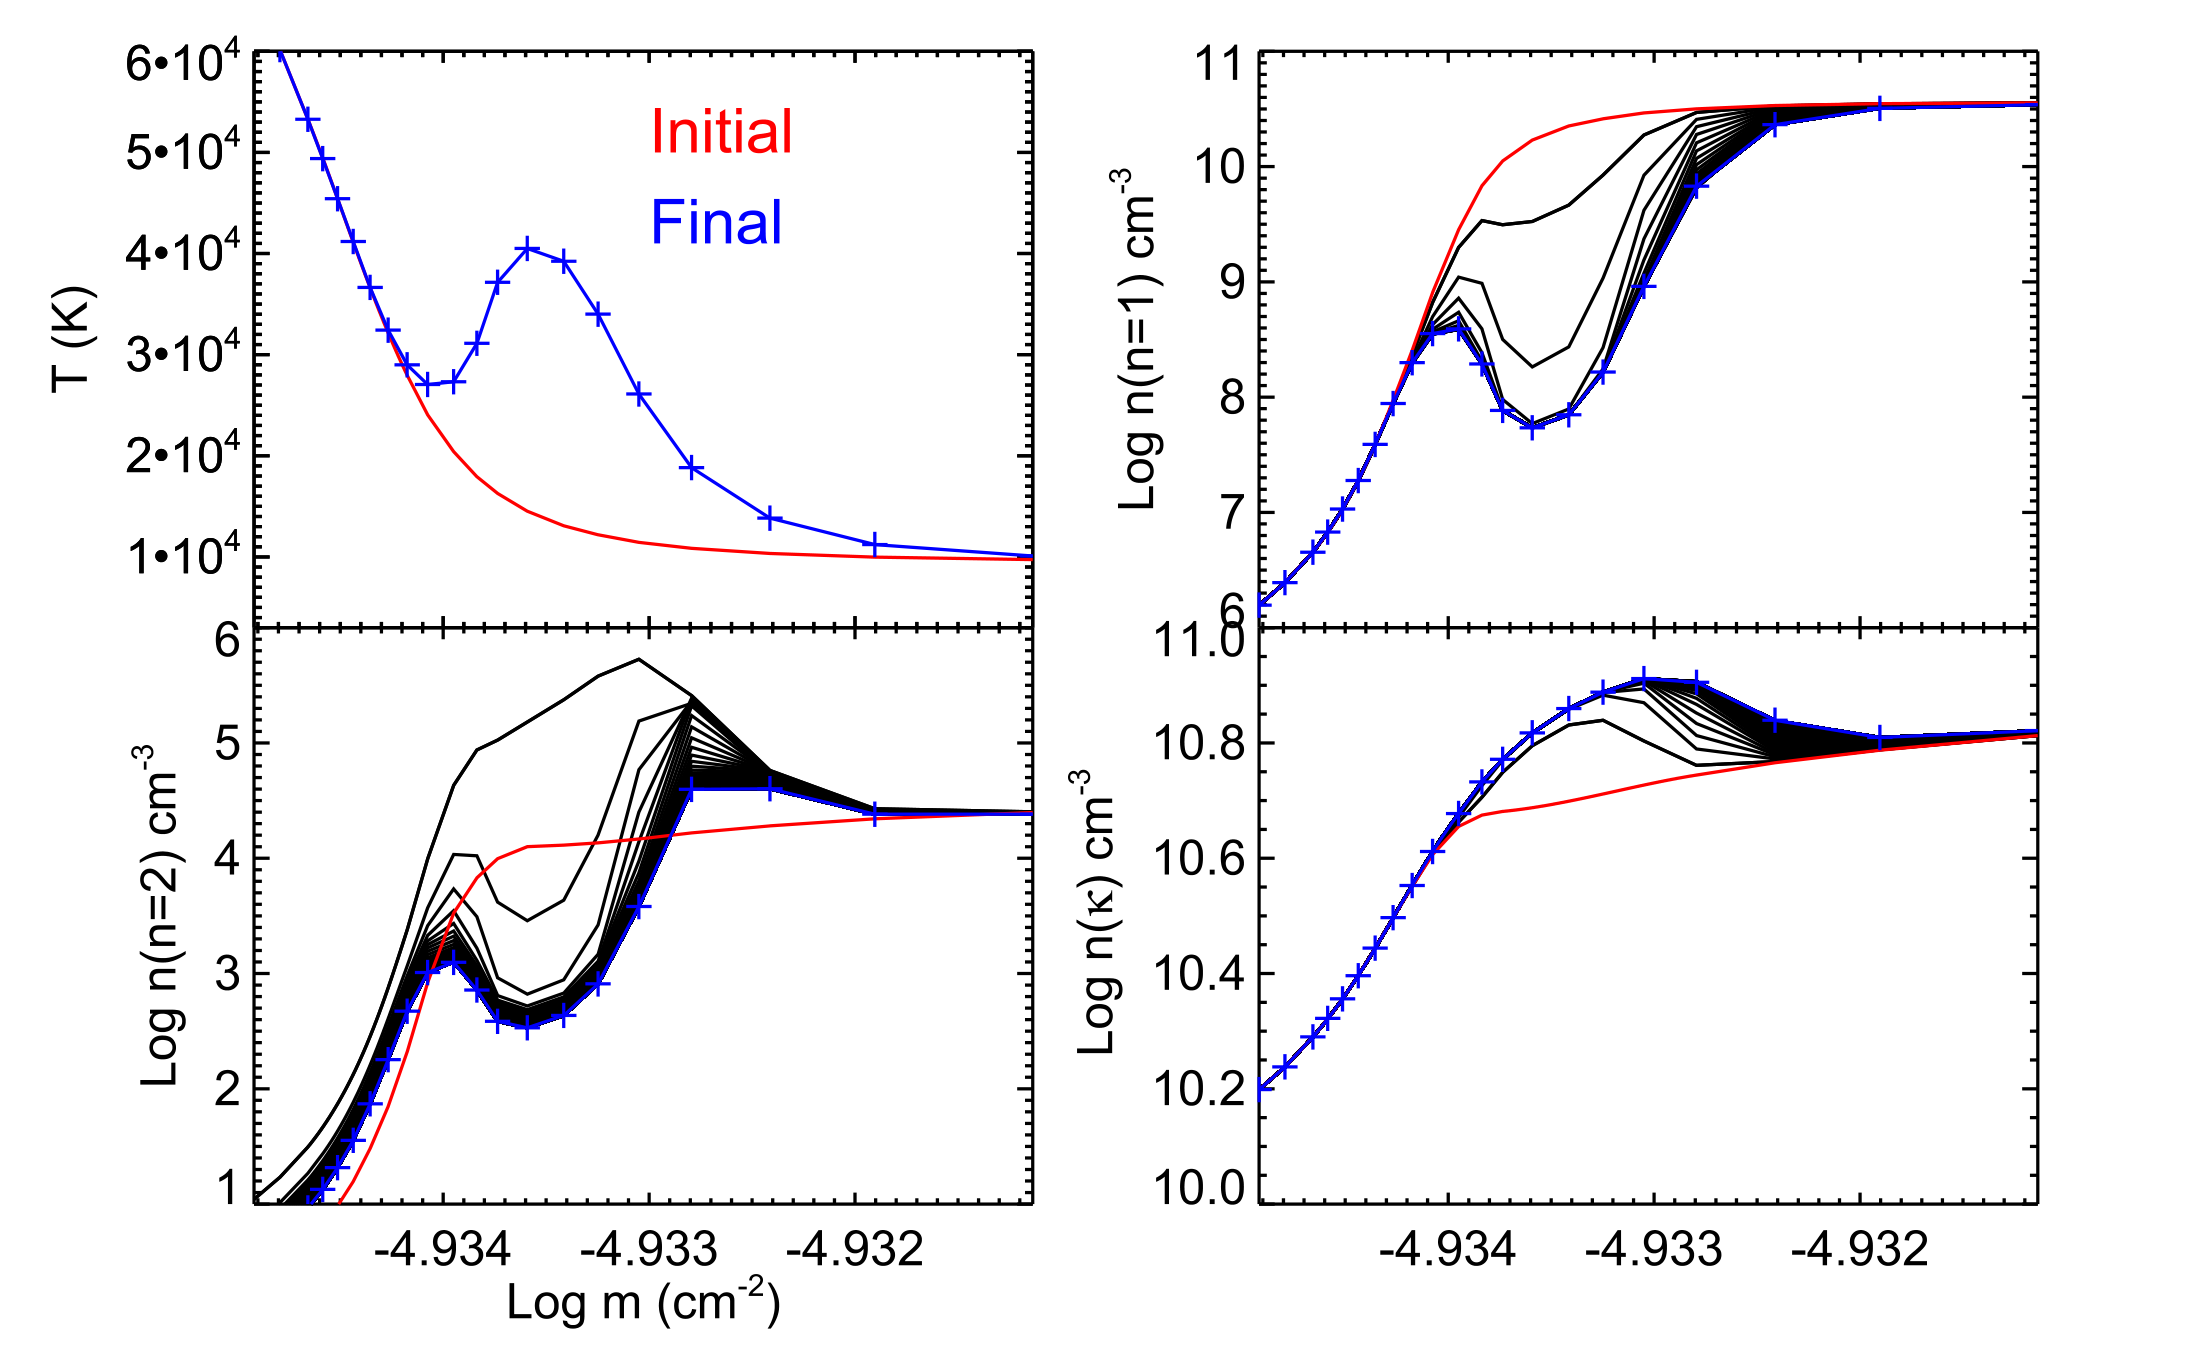
\includegraphics[width=0.85\columnwidth]{01aFlareModelling/StaticFigs/Judge2017Fig4.png}
    \caption[Fig. 4 of Judge (2017). Time-dependent response of hydrogen populations to instantaneous temperature change.]{Fig. 4 of \citet{Judge2017}. The response of hydrogen levels ($n=1, 2$) and continuum ($\kappa$) are shown for an instantaneous perturbation of the temperature of the FALC model (top-left panel). Each black line shows the population densities once every \SI{1}{\second}. © AAS. Reproduced with permission.}
    \label{Fig:Judge2017Original}
\end{figure}
\py[Lw]|chLw.get_figure('LwValidationJudge')|

Slightly more complex examples are needed to test the time-dependent machinery present in \Lw{}, and neither SNAPI nor RH, with their time-independent viewpoints can be used for comparison here.
We instead use the example of a perturbed FALC atmosphere presented by \citet{Judge2017}.
This figure is reproduced here as Fig.~\ref{Fig:Judge2017Original}.
After converging to the statistical equilibrium solution in a standard FALC atmosphere, the temperature is perturbed as shown by the blue line of the top-left panel of both Fig.~\ref{Fig:Judge2017Original} and our own solution presented in Fig.~\ref{Fig:LwValidationJudge}.
This model uses a three level plus continuum model hydrogen atom, and the populations of the ground, first excited, and continuum states are shown in the top-right, bottom-left, and bottom-right panels of these figures respectively.
The red line shows their starting values, and the blue line their final values after the simulation has been allowed to run for \SI{500}{\second} in the case of Fig.~\ref{Fig:Judge2017Original} and \SI{60}{\second} for Fig.~\ref{Fig:LwValidationJudge}, as we find the solution has stabilised by this point.
The black lines represent the solutions for each population every \SI{1}{\second}.
The $x$-axis on these plots is the atmospheric column mass, and Fig.~\ref{Fig:LwValidationJudge} is prepared in cgs to allow direct comparison to Fig.~\ref{Fig:Judge2017Original}.
The typically temperature-dependent (i.e. due to assuming a Maxwellian electron distribution) collisional ionisation and excitation ``strengths'' are fixed to their values at \SI{7000}{\kelvin} obtained using the method of \citet{Johnson1972} (P. Judge, \emph{private communication}; we note that the collisional \emph{rates} associated with these still scale with $\sqrt{T}$).

We see good overall agreement with \citet{Judge2017}, but the differences are larger than those presented in the previous figures.
The method used by \citet{Judge2017} is different to ours, and uses full preconditioning but with a $\Lambda$ operator based on the escape probability formalism of \citet{Hummer1982}, using a one-sided escape probability.
This approach is much more approximate than the full MALI treatment applied in \Lw{}, as it only performs the approximate formal solution at one wavelength per transition, and computes the integrals over wavelength and angle analytically.
The advantage of this treatment is that it is much less computationally intensive.
Thus, the use of this approximate method by \citet{Judge2017} is likely to be the origin of the differences between our results, and we find that the level populations converge to similar final solutions, at apparently similar rates.
The most substantial difference between our results is for the $n=2$ population: in Fig.~\ref{Fig:Judge2017Original}, the points close to a column mass of \SI{-4.9315}{\per\square\centi\metre} do not vary from their initial values, whereas in our model they change quite dramatically, with an enhancement of up to 2\,dex, leaving the range of the original plot, but converge close to the expected final solution.
This is likely an effect of downgoing radiation not being considered in the escape probability based formal solution of \citet{Judge2017}.
The maximum enhancement in this level also peaks higher than that seen in Fig.~\ref{Fig:Judge2017Original}, but rapidly drops towards the expected solution.
The downgoing radiation is also likely responsible for the offset of the final populations from the initial model in the \SI{-4.9315}{\per\square\centi\m} region that is not present, as the populations stay stable when the populations are advanced in time through the same process without the temperature perturbation, i.e. statistical equilibrium is maintained.
This simple example illustrates that \Lw{}'s behaviour is reasonable when applied to time-dependent problems, and the quality of its treatment will become apparent in the in-depth comparisons with \Radyn{} presented in Chap.~\ref{Chap:TimeDepRt}.

\py[Lw]|chLw.get_figure('LwValidationTimeDepNe')|

In Fig.~\ref{Fig:LwValidationTimeDepNe} we show the electron density in the lower atmosphere at four different timesteps of a \Radyn{} simulation where the radiative transfer (including self-consistent electron density) has been reprocessed using \Lw{}.
The techniques used here will be described in depth in Chap.~\ref{Chap:TimeDepRt}, and this figure is produced using the F9 model described in Sec.~\ref{Sec:CaiiRadynSims}.
The \Lw{} model presented is run with time-dependent charge conservation, maintaining self-consistency throughout the remainder of the simulation, whilst loading the other thermodynamic parameters from the \Radyn{} model at each timestep, and using these to compute the time-dependent population updates and self-consistent electron density.
Advection of the atomic populations and electron density is performed using a similar technique to \Radyn{}, implemented as per Sec.~\ref{Sec:MsLwAdvection}.
The electron density in the \Radyn{} model is shown in blue, and the \Lw{} model in dashed orange.
The agreement between the two models is extremely good, including the fine features around $z=\SI{1.2}{\mega\metre}$ shown in the \SI{11}{\second} panel.

\Lw{} agrees well with the other models against which it has been tested here; it is easy to construct new validation tests for statistical equilibrium cases that can be run with many different extant radiative transfer codes, but the validation of time-dependent treatments on their own is more difficult, due to current tools often coupling these equations to hydrodynamics.
Other tests have been undertaken to verify the performance of \Lw{}, but those presented here should be sufficient to demonstrate its capabilities.


\section{\emph{Lightspinner}}

During the development of \Lw{}, a simpler pedagogic framework was also constructed.
This framework, \emph{Lightspinner}\footnote{Developed on GitHub (\url{https://github.com/Goobley/Lightspinner}), with archival on Zenodo.} \citep{Lightspinner}, is written in pure Python and focuses on documenting the internal numerics of a simple formal solver and the MALI method using full preconditioning (under the assumption of CRD).
It is accompanied by a slide deck highlighting the most important terms that need to be understood to implement these methods following \citet{Rybicki1992} and \citet{Uitenbroek2001} for iteration, and \citet{Olson1987} and \citet{Auer1994} for the short-characteristics formal solver (although only a linear formal solver is implemented in the code). This framework can be employed to help users familiarise themselves with the concepts of NLTE radiative transfer and some of the techniques present in \Lw{}; it presents the core concepts clearly, and naïvely, without focusing on performance, so can easily be dismantled and understood by a single person over the course of a few days.

\section{Discussions}

We have presented a description and validation of the \Lw{} radiative transfer framework and the intentions behind its design.
Frameworks can substantially enhance productivity, and enable the construction of specialised tools without the need to focus on the implementation or performance of the common core of dense numerical code shared by programs of this style.
The power of this will be demonstrated with the experiments presented in Chapters~\ref{Chap:TimeDepRt} and \ref{Chap:2DRT} which leverage \Lw{} significantly, and demonstrate how the addition of small amounts of Python can yield tools that would otherwise require in-depth modification and coupling of existing tools such as RH and \Radyn{}.
\chapter{Time-Dependent Radiative Transfer}\label{Chap:TimeDepRt}
%TC:group pycode 0 0
\setpythontexautoprint{false}
\begin{pycode}[TimeDepRT]
name = 'TimeDepRT'
chRT = texfigure.Manager(
    pytex,
    './02TimeDepRT',
    number=2,
    python_dir='./02TimeDepRT/python',
    fig_dir=   './02TimeDepRT/Figs',
    data_dir=  './Data/02TimeDepRT'
)
\end{pycode}

% \begin{pycode}[TimeDepRT]
% from lightweaver.fal import Falc82
% from lightweaver.rh_atoms import H_6_atom, C_atom, O_atom, Si_atom, Al_atom, CaII_atom, Fe_atom, He_atom, MgII_atom, N_atom, Na_atom, S_atom
% import lightweaver as lw
% import matplotlib.pyplot as plt
% import numpy as np

% def iterate_ctx(ctx, Nscatter=3, NmaxIter=500):
%     for i in range(NmaxIter):
%         dJ = ctx.formal_sol_gamma_matrices()
%         # NOTE(cmo): Do some initial iterations without touching the
%         # populations to lambda iterate the background scattering terms
%         if i < Nscatter:
%             continue
%         delta = ctx.stat_equil()

%         # NOTE(cmo): Check convergence
%         if dJ < 3e-3 and delta < 1e-3:
%             print('Iterations taken: %d' % (i+1))
%             print('-'*60)
%             return

% wave = np.linspace(853.9444, 854.9444, 1001)
% def synth_8542(atmos, conserve, useNe):
%     # NOTE(cmo): Configure the Gauss-Legendre angular quadrature for 5 rays
%     atmos.quadrature(5)

%     # NOTE(cmo): Construct the RadiativeSet with the following atomic models
%     aSet = lw.RadiativeSet([H_6_atom(), C_atom(), O_atom(), Si_atom(), Al_atom(), CaII_atom(),
%                             Fe_atom(), He_atom(), MgII_atom(), N_atom(), Na_atom(), S_atom()])
%     # NOTE(cmo): Set Hydrogen and Calcium to active
%     aSet.set_active('H', 'Ca')
%     # NOTE(cmo): Compute the SpectrumConfiguration for this RadiativeSet
%     spect = aSet.compute_wavelength_grid()

%     # NOTE(cmo): If we're using the electron density provided with FAL C, then
%     # compute the associated LTE populations, otherwise find a solution for
%     # self consistent LTE populations and electron density.
%     if useNe:
%         eqPops = aSet.compute_eq_pops(atmos)
%     else:
%         eqPops = aSet.iterate_lte_ne_eq_pops(atmos)

%     # NOTE(cmo): Construct the Context, optionally setting chargeConservation and the number of threads to use.
%     ctx = lw.Context(atmos, spect, eqPops, conserveCharge=conserve, Nthreads=8)

%     # NOTE(cmo): Iterate the NLTE problem to convergence
%     iterate_ctx(ctx)
%     # NOTE(cmo): Compute a detailed solution to Ca II 8542 on the 1 nm wavelength grid above
%     Iwave = ctx.compute_rays(wave, [1.0], stokes=False)
%     return Iwave

% # NOTE(cmo): Load an atmosphere. In this case we include a copy of FAL C, but
% # Lightweaver also supports loading atmospheres in the MULTI format, and it is
% # also simple to do so from the raw data components
% atmosRef = Falc82()
% # NOTE(cmo): Ca II 8542 with the reference electron density in the FAL C atmosphere
% IwaveRef = synth_8542(atmosRef, conserve=False, useNe=True)

% atmosCons = Falc82()
% # NOTE(cmo): Ca II 8542 with the electron density obtained from charge conservation
% IwaveCons = synth_8542(atmosCons, conserve=True, useNe=False)

% atmosLte = Falc82()
% # NOTE(cmo): Ca II 8542 with LTE electron density
% IwaveLte = synth_8542(atmosLte, conserve=False, useNe=False)

% fig = plt.figure()
% plt.plot(wave, IwaveRef, label='Reference')
% plt.plot(wave, IwaveCons, '--', label='Conserved')
% plt.plot(wave, IwaveLte, '--', label='LTE')
% plt.title(r'Comparison of Ca\,\textsc{ii} 854.2\,nm with different electron densities', y=1.04)
% plt.ylabel(r'Intensity [SI]')
% plt.xlabel(r'$\lambda$ [nm]')
% plt.legend()
% lFig = chRT.save_figure('EleDensComparison', fig, fext='.pgf')
% lFig.caption = r'Comparison of Ca\,\textsc{ii} 854.2\,nm with different electron densities'
% \end{pycode}
% \setpythontexautoprint{false}

% \py[TimeDepRT]|chRT.get_figure('EleDensComparison')|

% \begin{itemize}
%     \item Current problems not solved by RADYN and MS\_RADYN.
%     \item \Lw{}
%     \item \MsLw{}
%     \item Reprocessing RADYN simulations
%     \item Effect of the Lyman lines on \CaLine{} in RHD simulations
%     \item Diagnostic potential of response functions
%     \item Another item - PRD is hard?
% \end{itemize}

Modern Radiation Hydrodynamic (RHD) codes are highly complex, and contain many specialised features as discussed in the previous chapter.
In the following discussion we will focus primarily on \Radyn{}, the most widely used code of its ilk, and how using additional tools can facilitate new avenues of investigation.

\TODO{Explicit vs implicit}

\TODO{2 subcomponents}

\section{A Brief Dissection of \Radyn{} and the Future of RHD Modelling}\label{Sec:RadynDissection}

\emph{This section is informed by my discussions with Mats Carlsson, experiences using \Radyn{}, and in-depth analysis of its source code. It represents my own conclusions from the synthesis of these.}

\Radyn{}'s design closely follows its radiative transfer lineage. Its direct predecessor is the MULTI radiative transfer code and many commonalities remain.
NLTE radiative transfer is solved on a per transition basis using an ALI method and linearisation of the resultant level population balance equations.
This method is designed to solve the problem of non-overlapping lines but including an underlying background continuum.
This linearisation approach was proven by \citet{SocasNavarro1997} to be effectively equivalent to that of preconditioning for non-overlapping transitions \citep{Rybicki1991} for pure radiative transfer problems in the statistical equilibrium case.
This approach also assumed the use of a local diagonal $\Lambda^*$ operator, as discussed in the previous chapter.
\Radyn{}, however, chooses to employ a pentadiagonal $\Lambda^*$ operator to make optimal use of matrix bandwidth necessary elsewhere in the program and obtain improved convergence as a result.
It is unlikely that this change in operator significantly affects the conclusions of \citet{SocasNavarro1997}, but affects the two methods will no long arrive at the exactly equivalent numerical formulations.

The advantage of the linearisation approach in \Radyn{} is the ability to directly couple other equations to the RTE and implicitly solve all of these simultaneously and self-consistently.
Taking for example the kinetic equilibrium equation \eqref{Eq:KinEq}, \Radyn{}'s method formulates this expression such that the corrections from both the advection and population transition terms are considered simultaneously.
This is achieved through the use of a Newton-Raphson method, where the Jacobian is computed based on an analytic derivation, including the aforementioned linearisation of the kinetic equilibrium equation.
This same process simultaneously solves for the heat conduction, hydrodynamics of the system, and the new locations of the dynamic grid of \citet{Dorfi1987}.

A significant benefit of this implicit approach is a relaxation of the timestep constraints present in explicit approaches.
This is particularly important when considering the very fine grid spacing often required by the dynamic grid, which combined with the large bulk velocities occurring in flares can lead to extremely oppressive timestep constraints.

Despite its elegance, there are several major downsides to this implicit approach.
Foremost of these is the complexity engendered by the coupled design of the system, and the need to ensure that all necessary derivatives are analytically computed and included.
This presents a very large barrier to entry for future developments on the platform, and this is likely part of the reason why both Fokker-Planck modules integrated in \Radyn{} have operated externally to this core coupled system.
This overlapping of concerns
Additionally, implicit codes, whilst having reduced timestep constraints, are typically much more costly per timestep than explicit codes.
This is somewhat offset by the majority of the cost of each step residing within the formal solver, which remains similar in both cases.
The dynamic grid can also become problematic due its lack of interpretability, and propensity to drop to spacings finer than the local cyclotron radius in more energetic simulations.

\Radyn{} is a fantastic tool that has enabled insight into many different flare associated phenomena, and through these comments we do not intend to discredit its use, but instead highlight avenues for future development within the field of RHD.
As the different uses of \Radyn{} continue to evolve in complexity, with projects such as multi-strand arcade and minority species modelling \NeedRef{}, the code at the core of \Radyn{} will need to be modified by different researchers, and work facilitating this and highlighting additional factors to be considered in RHD modelling is core to the future development of this field.

As discussed previously in respect to \Lw{} and radiative transfer, the flexibility of a framework designed for solving a class of problem can yield significant advances in productivity.
The task of designing, constructing, and testing such a framework for a problem such as the complete quasi-one-dimensional RHD simulation flares is too significant to be undertaken here.
Nevertheless, it may prove a convenient future development once the necessary specifications are defined.
Here, we focus on reprocessing aspects of the radiative transfer of previously computed \Radyn{} simulations and investigate important directions for future developments in RHD modelling of flares.

\section{Minority Species}

For flares, \Radyn{}'s primary focus is on the major spectral lines and continua of hydrogen, helium, and calcium.
These typically represent the bulk of the radiative energy lost in the chromosphere.
Singly ionised magnesium has also been shown to be an important contributor to these energy losses, however the h and k lines require a treatment including PRD to avoid significantly overestimating their losses.
The \Caii{} H and K lines are also somewhat affected by PRD, in addition to the hydrogen Lyman lines.
For the Lyman lines we will discuss several strategies for approximating this treatment, and for \Caii{} H and K, it has been suggested that considering these in CRD approximately accounts for the lack of Mg\,\textsc{ii} h and k if all of these transitions were treated with PRD \citep{Kerr2019a}.

Whilst the lines of these four species are some of the strongest in solar spectrum, and their continua mediate much of the energy leaving the chromosphere, there are other chromospheric transitions that can also be used to diagnose the atmosphere.
For example, Si\,\textsc{iv} optical thickness has been investigated in a minority species context by \citet{Kerr2019c}.
An element treated as a ``minority species'' is assumed to not interact significantly with the energy balance of the simulation (i.e. the thermodynamic response of the model does not change significantly if this species is subject to a complete radiative treatment).
This should be true for most species with trace populations.
The radiative transfer calculations associated with this species can then be performed in a ``second-pass'' over a previously computed \Radyn{} simulation.
The MS\_RADYN code was designed for this task; it takes the thermodynamic parameters from every timestep of a \Radyn{} simulation, along with the non-equilibrium hydrogen populations, and solves the kinetic equilibrium equation at each timestep for a minority species.
Due to the lack of atmospheric thermodynamic response to changes in the radiative output of this species, far more complex atomic models can be used, such as the 30 level model silicon atom used by \citet{Kerr2019c}.

An approach similar to that of minority species modelling can be applied to testing the methods used in \Radyn{} and the importance of certain omissions.
Due to the reduced complexity of solving the kinetic equilibrium equations rather than the entire RHD system, these calculations typically run significantly faster than the original simulation.
In the following we will discuss the creation of a minority species tool for reprocessing \Radyn{} simulations, built on the \Lw{} framework, as well as its application to investigating the importance of overlapping transitions and discussing the difficulties of including PRD in these simulations.
From the previous discussion, building such a tool on the \Lw{} framework should provide researchers with a modern, simpler codebase that is easier to conceptualise and modify, allowing for investigation of effects to be included in \Radyn{} or future RHD codes.
Excluding the model atom definitions, the source code of the simulations presented in this chapter totals $\sim$1000 lines of Python, mostly following modern best practices.

\section{Reprocessing \Radyn{} Simulations with the \Lw{} Framework}

To perform a minority species simulation, a particular file from the original simulation, \texttt{atmost.dat}, must be provided.
From investigating the contents of this file we can determine the exact configuration of \Lw{} and the equations to be solved.
This file is written to for every internal timestep of the \Radyn{} simulation, and represents a limited subset of the less frequently written ``complete'' output (typically stored every \SI{0.1}{\second}).
It contains some metadata describing the size of the simulation, then for each internal timestep, the current timestep, the elapsed time at each timestep, the current locations of the dynamic grid, the mass density profile, the electron density profile, the temperature structure, the vertical velocity, and the current hydrogen level populations.

For the validation of \Lw{} and this style of simulation, we also wished to compute and compare the hydrogen populations to those computed in \Radyn{}.
Several difficulties arose due to the non-thermal collisional rates used in the kinetic equilibrium calculation for hydrogen and helium.
The non-thermal collisional rates of \citet{1993Fang} are used to determine hydrogen ionisation, and require the beam energy deposition throughout the atmosphere at each timestep.
For helium, if the Fokker-Planck electron beam description is used, then the rates of \citet{Arnaud1985} are used, but these require integration over the electron energy distribution.
Whilst it is possible to add both of these to the \texttt{atmost.dat} file, the complete electron distribution information is very large, and we instead elect to use ``Emslie'' beam electron formalism \citep{Emslie1978}, for which the energy deposition profile throughout the atmosphere is sufficient to describe the non-thermal rates.
We therefore chose to slightly modify \Radyn{} and add the beam heating profile to the \texttt{atmost.dat} file.
Our function for reading these files can handle both files with and without this modification.
In the event that this beam heating information is not saved, an approximation of it can be reconstructed via interpolation from the information in \Radyn{}'s complete save file.
Our testing of this show that the approximation is relatively good, but short term, or particularly narrow heating features may be lost.
For this reason, all simulations presented here use the version with this data.

With the above data we have sufficient information to construct the \Radyn{} thermodynamic atmosphere at any of its internal timesteps.
\Lw{} does not make use of the mass density directly, but instead maps it to hydrogen density.
For this we use of the default abundances in \Lw{}, based on \citet{Asplund2009}.
These differ to those used in \Radyn{}, but not significantly for any of the species discussed here.
Ignoring the advection term it is then simple to produce a minority species tool using this approach.
In many situations, the advection term has a small effect, and can safely be ignored \NeedRef{} \TODO{Old Flarix paper}.
The radiative transfer equation employed in \Radyn{} is formulated on the dynamic grid, and this is not the case in \Lw{}, which assumes that the grid is static (although this limitation can be worked around).
We can simply use a fixed denser spatial sampling of the atmosphere to account for the motion of features such as the transition region over the course of the simulation.
This model then interpolates the thermodynamic properties and NLTE hydrogen populations for the starting atmosphere onto our stratification and computes the statistical equilibrium solution for the minority species in question.
For each subsequent timestep these properties are interpolated from the new \Radyn{} grid to the static grid, and the minority species populations can be advanced in time using the process described in Sec.~\NeedRef{}.

To reduce the number of grid points needed for a static stratification one could instead use a fixed column mass stratification.
The transition region moves very little in terms of column mass during the simulation, however it then becomes necessary to interpolate the populations from one column mass stratification to the next; a process which can introduce significant error if not undertaken with care.
This error can be reduced by renormalising each specie's total number density throughout the atmosphere from the mass density and abundances, and this helps to avoid errors growing around regions of high gradient, such as the transition region.

To solve the minority species problem properly in a manner compatible with \Radyn{} it is necessary to include the advection terms.
In the following we will describe several different approaches to handling these advection terms, and thus solving the complete kinetic equilibrium equations.

\subsection{Advection}

In Sec.~\ref{Sec:RadynDissection} we discussed the coupled nature in which \Radyn{} solves the RHD equations.
For flexibility we wish to decouple the advection terms from the population transitions.
Our initial approach was to use an explicit method on the dense, fixed grid discussed above.
Explicit methods are typically simpler to validate and understand, so seemed a logical fit for this project.

\TODO{Describe WENO-HD -shocks etc}

To improve the agreement with \Radyn{}, reduce the number of interpolations,. and leverage its adaptive grid we instead decided to apply its technique for advection, but keep it distinct from the radiative transfer.
Thus, at the start of each timesteps we advect the populations from the previous grid to the new grid locations, and then advance the populations in time based on the NLTE rates.
This technique is known as operator splitting \NeedRef{}, and is commonly applied in hydrodynamics simulations where different numerical techniques are effective at solving different components of the system.
Performing a na\"{i}ve splitting like this limits the accuracy of the solution to first order accuracy in time.
Various advanced splitting techniques, such as Strang splitting \citep{Strang1968}, have been developed to reduced this error.
Strang splitting reduces these error terms to second order, and newer approaches can reduce the impact of operator splitting to fourth order in time \NeedRef{}.
A Strang splitting approach was implemented in our code using these components, but the results were not found to differ appreciably.
It is likely that this is due to one of the two processes dominating.
During explosive heating the populations in the upper chromosphere typically have very large transition rates, and comparatively slow advection.
At later times, when the timestep is longer, the transition rate is typically much lower and the plasma flows are relatively smooth, but often high velocity.

As discussed above, it is necessary to accurately and conservatively resolve shocks in advection and hydrodynamics problems, something that has been recognised since the 1950s \NeedRef{} \TODO{FCT book?}.
For this \Radyn{} employs a variant of the second order spatially accurate method of \citet{VanLeer1979}.
The concept of this class of method is similar to that of short characteristics formal solvers, ensuring that no spurious minima or maxima are injected into the solution, which in hydrodynamics would result in a gain or loss of density.

\TODO{I think we need a clear introduction to shock capturing methods. Read over pyCLAW paper and Leveque intro.}
\chapter{Two-Dimensional Radiative Transfer}
%TC:group pycode 0 0
\begin{pycode}[2DRT]
name = '2DRT'
ch2DRT = texfigure.Manager(
    pytex,
    './03TwoDRT',
    number=3,
    python_dir='./03TwoDRT/python',
    fig_dir=   './03TwoDRT/Figs',
    data_dir=  './Data/03TwoDRT'
)
\end{pycode}

% \begin{itemize}
%     \item Adding a dimension to RT, formal solver etc.
%     \item Simulation setup.
%     \item Analysis.
%     \item Suggestions on visibility of this chromospheric glow with DKIST.
% \end{itemize}

It is clear that the world around us is multi-dimensional, but until this point, we have only considered radiative transfer in one-dimensional atmospheres.

All of the theory of radiative transfer discussed in previous chapters remains valid when applied to higher dimensional systems, with the exception of the description of the formal solver.
This is due to the non-local terms that appear within the MALI description (with diagonal $\Lambda$ operator) being handled by formal solver, which is responsible for computing the radiation field throughout the plasma from the local parameters and boundary conditions and thus coupling the atmospheric nodes to each other.
Once the radiation field has been computed it is then used as a local parameter in the rest of the iteration.
In fact, if the storage for the atmosphere is ``flattened'' into a one-dimensional form, the code from the plane-parallel case can (and should) be used to implement the iteration scheme.

In this chapter we shall first describe the extension of the \Lw{} framework to two dimensions (with the possibility of further extension), and then describe its application to the simulation of a flaring atmosphere illuminating an adjacent slab of quiet sun, along with potential implications for future observations at high resolution.

\section{The Formal Solver in Two-Dimensions}

Similarly to the plane-parallel formal solver used in \Lw{}, described in the previous chapter, we use the short-characteristics method to compute the radiation field throughout the atmosphere.
This approach was first employed in two-dimensions by \citet{Auer1994} using a limited parabolic scheme to avoid overshoot.
We assume the following basis: the $z$-axis is oriented as in the plane-parallel case, oriented vertically from photosphere to corona, the $x$-axis is perpendicular and co-planar to the $z$-axis (in the plane of the page for the following diagrams), and by the right-hand rule the $y$-axis is oriented into the plane of the page.
In the two-dimensional case it is assumed that the atmospheric parameters are homogenous along the $y$-axis, but vary along the $x$- and $z$-axes.
We assume that the atmosphere has a fixed stratification in $x$ and $z$, and that the atmospheric parameters are known at each intersection of these grids.

The mean intensity at each point will be computed similarly to the plane-parallel case; by integration of the local intensity over a weighted angular quadrature.
The Gauss-Legendre nodes used in the plane-parallel case are poorly suited to anisotropy that occurs in the two- and three-dimensional cases, and so we therefore employ the optimised quadratures of \citet{Stepan2020} in \Lw{}.

\begin{figure}
\centering
\begin{tikzpicture}[scale=1.5, line width=1pt, >=latex]
    \def\xcoords{1,2,3.5,4,5}
    \def\xmax{5}
    \def\ycoords{1,2,2.5,3.5,5,6}
    \def\ymax{6}
    \def\raym{4/3}
    \def\rayc{-7/6}

    \draw [help lines]
    \foreach \y in \ycoords {
        (1, \y) -- (\xmax, \y)
    }
    \foreach \x in \xcoords {
        (\x, 1) -- (\x, \ymax)
    };
    \draw [<->] ({\xmax+0.5}, 1) node[below] {$x$} -- (1,1) -- (1, {\ymax+0.5}) node[left] {$z$};
    \coordinate (O) at (3.5, 3.5);
    \node[circle, fill=black, inner sep=0 pt, minimum size=3pt, label=above left:{$O$}] at (O) {};
    \draw[->, domain=1.8:4.8, samples=10, thin] plot(\x, {\raym * (\x) + \rayc});
    \coordinate (D) at (4, {\raym * 4 + \rayc});
    \node[circle, fill=black, inner sep=0 pt, minimum size=3pt, label=right:{$D$}] at (D) {};
    \coordinate (U) at ({(2.5 - \rayc) / (\raym)}, 2.5);
    \node[circle, fill=black, inner sep=0 pt, minimum size=3pt, label=above left:{$U$}] at (U) {};

    \node[circle, fill=black, inner sep=0 pt, minimum size=2pt, label={[label distance=0.5mm]above left:{\small $\alpha$}}] at (2, 2.5) {};
    \node[circle, fill=black, inner sep=0 pt, minimum size=2pt, label={[label distance=0.5mm]above right:{\small $\beta$}}] at (3.5, 2.5) {};
    \node[circle, fill=black, inner sep=0 pt, minimum size=2pt, label={[label distance=0.5mm]below right:{\small $\gamma$}}] at (4, 3.5) {};
    \node[circle, fill=black, inner sep=0 pt, minimum size=2pt, label={[label distance=0.5mm]above right:{\small $\delta$}}] at (4, 5) {};
\end{tikzpicture}
\caption{Diagram of short characteristics scheme in two-dimensions.}
\label{Fig:Sc2d}
\end{figure}

For each ray prescribed by the angular quadrature the formal solver must perform one sweep through the grid.
The general case, that of an inclined ray ray travelling through the atmosphere is shown in, Fig.~\ref{Fig:Sc2d}.
In the case of this ray the formal solver must sweep first along $x$ and then along $z$, and the difficulties which can arise from this will be discussed in Sec.~\ref{Sec:2dEvalOrder}.
The points $U$ and $D$ refer to them being ``upwind'' and ``downwind'' of the point $O$ for which we are currently computing the intensity.
This can be explained by looking at the intersections of ray with the grid.
To compute the intensity in the direction of this ray at point $O$ using the short characteristics formulation we have, as in one-dimension,
\begin{equation}\label{Eq:MiniScDefinition}
   I_O = I_U e^{-(\tau_U - \tau_O)} + \int_{\tau_O}^{\tau_U} S(t) e^{-(t - \tau_O)}\, dt,
\end{equation}
where these terms have their usual meanings, $I_O$ is the intensity in this direction at $O$, $I_U$ is the intensity in this direction at $U$ and we have dropped the angular and frequency dependencies for clarity.
Thus, to compute the intensity at $O$, the intensity at $U$ must first be known.
As $U$ does not typically lie on a point of our discrete two-dimensional grid, the value of $I_U$ (and other quantities) are not computed directly by the formal solver, and must instead be interpolated from the values of grid points along the line $\alpha\beta$.

Following the short characteristic method, a functional form must be assigned to the variation of $S$ over the the line segment $[UO]$.
In the simplest case, this can again be a linear functional form, but due to the additional dimension for inhomogeneities in the two-dimensional case, unless the grid is very fine or the atmosphere very slowly varying, this may be a poor choice.
A higher order parametrisation of $S$ is likely to require the values of the source function at both $U$ and $D$, and possibly other points along this path.
Similarly to the cubic Bézier spline method used as standard in our plane-parallel code, we once again turn to monotonic Bézier splines for safe, smooth interpolation, minimising the presence of under and over-shoots.
The cubic method we apply in plane-parallel atmospheres requires four points along $UD$, which becomes less practical in higher dimensions, due to the large computational demands of the method.
Instead we choose the quadratic Bézier spline method, BESSER, of \citet{Stepan2013}, which will be briefly summarised here for the scalar case of the RTE.

\subsection{The BESSER method}

The BESSER method differs from other quadratic Bézier spline methods by ensuring the continuity of the first derivative of the interpolant at $O$.
Due to the large differences in optical depth between adjacent regions (e.g. $\tau_{UO}$ and $\tau_{OD}$) that are likely to occur in multi-dimensional cases with irregular grids, this method is designed so as to guarantee that if the values over $[UOD]$ are monotonic then the spline interpolant will remain monotonic.

The spline interpolant over the $[UO]$ interval is described by
\begin{equation}
    f(u) = (1-u)^2f_U + 2u(1-u)c_U + u^2f_O,\hspace{3em}u\in[0,1],
\end{equation}

where $f$ is the value of the parameter to be interpolated, $c_U$ is the functional value of the spline's control point, and $u$ is the normalised coordinate for the distance along $[UO]$.
The control points are points half way along an interval, defining the tangent to the spline at each end of the range i.e. $c_U O$ defines the tangent to the spline at $O$ and $U c_U$ defines the tangent to the spline at $U$.
If we denote the coordinates of our points along the ray $s_U$, $s_O$, and $s_D$ then we have $u = (s - s_U) / h_U$, where $h_U = s_U - s_O$.
An equivalent interpolation can be defined over the $[OD]$ segment.
The monotonicity (for monotonic $f_U$, $f_O$, $f_D$) and continuous first derivative of the interpolating functions at $O$ is ensured by
\begin{enumerate}
    \item Verify the monotonicity of $f_U$, $f_O$, $f_D$, and if $f_O$ is a local extremum then the control points $c_U$ and $c_D$ are set to $f_O$, giving a derivative of zero at $O$. As this is is the only possible solution for this case, the process stops here.

    \item Compute an estimate of the derivative at $O$, by using the derivative of the standard parabolic interpolation of $UOD$.

    \item Use this derivative to compute the initial values at the control points, by direct projection of the first derivative to their coordinates (as this defines a tangent to function at $O$).

    \item Check $c_U \in [f_U, f_O]$. If not, set $c_U$ to $f_U$ to correct for any new extremum and halt the process, as $c_D$ is not needed for the integration of the source function.

    \item Check $c_D \in [f_O, f_D]$. If not, set $c_D$ to $f_D$, and use this to compute a new value for the derivative at $O$, and follow the projection of this tangent to determine $c_U$ (due to the enforced continuity of the derivative at $O$).
\end{enumerate}
This process is described in more detail in \citet{Stepan2013}, but this covers the most important elements of the process.

\TODO{Do we modify to use the full value for $\tau_{OD}$?}
\TODO{Is this the correct what of expressing the difference between the control point, and the \emph{value} of the control point?}

Similarly to the plane-parallel case, we will solve the RTE in optical depth, due to its increased stability.
This interpolation method can be used to compute $\tau_{UO}$ and $\tau_{OD}$ by
\begin{align}
    \tau_{UO} &= \frac{1}{3}(\chi_U + \chi_O + \chi_{c_U}) (s_O - s_U),\\
    \tau_{OD} &= \frac{1}{2}(\chi_O + \chi_D) (s_D - s_O).
\end{align}
Note that a linear approximation was used for $\tau_{OD}$, as the previous process does not guarantee the calculation of $c_D$.
This could be modified to also use the quadratic spline method, which may be more robust, however the value of $\tau_{OD}$ rarely affects the final solution dramatically.

This method can now be applied to the source function but parametrised along $\tau$ rather that $s$.
The BESSER quadratic spline method is then used to compute the value of the source function control point $S_{c_U}$.
The integral in \eqref{Eq:MiniScDefinition} can now be evaluated, by using the prescribed quadratic spline variation of $S$ over the interval $[\tau_{U}, \tau_{O}]$.
Working through the maths we arrive at
\begin{equation}
    I_D = I_Ue^{-\tau_{UO}} + \omega_U S_U + \omega_O S_O + \omega_{c_U} S_{c_U},
\end{equation}
where,
{
\def\edt{e^{-\tau_{UO}}}
\def\tsq{\tau_{UO}^2}
\begin{align}
    \omega_U &= \frac{2 - (\tsq + 2\tau_{UO} + 2)\edt}{\tsq},\\
    \omega_O &= 2\frac{\tau_{UO} - 2 + \edt (\tau_{UO} + 2)}{\tsq},\\
    \omega_{c_U} &= 1 - 2 \frac{\edt + \tau_{UO} - 1}{\tsq}.
\end{align}
}

For small values of $\tau_{UO}$ the numerical precision of the exponential function becomes unreliable (in floating point arithmetic), so for this reason these are replaced with Taylor expansions for $\tau_{UO}\lesssim 0.1$.

An expression for the $\Lambda^*$ operator can then be devised equivalently to the process used previously for the plane-parallel case.
The source function is locally set to unity, and zero elsewhere.
This implies that $c_U$ is also set to 1.
Thus the local contribution to the radiation field is given by
\begin{equation}
    \Lambda^*(\nu, \vec{d}) = \omega_{c_U} + \omega_O,
\end{equation}
and remains related to $\Psi^*$ by the local opacity.

The equivalent integration and $\Lambda$ operator coefficients for a linear short characteristics approach can be computed similarly and are analagous to those computed in the one-dimensional case.

\subsection{Evaluation Order and Boundary Conditions}\label{Sec:2dEvalOrder}

Looking more closely at the order in which the formal solver needs to sweep the grid, we can see that the point $O$ for the ray discussed in the previous section (and shown in Fig.~\ref{Fig:Sc2d}) would be the 10th node to be solved, and this ordering is shown in Fig.~\ref{Fig:2DSweep}.
Most of the nodes on this figure are solved equivalently to this one, with all necessary quantities known at evaluation time provided the sweep order is preserved, but there are several question marks which require explanation.

\begin{figure}
\centering
\subimport{03TwoDRT/}{SweepOrder}
\caption{Diagram of sweep order in 2D}
\label{Fig:2DSweep}
\end{figure}

The {\color{TolBlue} blue} question marks along the $x$ axis all require values that must be computed from the boundary conditions.
The upper and lower boundary conditions in $z$ are typically taken to be described by a defined in-going radiation field (possibly zero or based on a black body).
The upper and lower boundaries in $x$ can be described by fixed boundary conditions, but it is also common to describe these with periodic boundary conditions where the ray wraps from one side of the grid to the other.
The {\color{TolTeal} teal} question marks along the upper $x$ boundary can then be interpreted in multiple ways; in the case of periodic boundary conditions they can be prolonged along the {\color{TolTeal} teal} arrows, and used in the same way as the previously described case.
If fixed boundary conditions are used then the intensity at these points must be computed by a linear formal solver indicated by the black arrows ending at the nodes labelled 4 and 8.

Finally, the region around the {\color{TolOrange} orange} question mark, the tail end of the arrow passing through node 11, requires some additional explanation.
In the configuration shown here, the arrow can stop at its intersection with the vertical line on which nodes 6 and 10 lie as the intensity information has been computed at both of these.
If an equivalent situation occurs at a periodic $x$ boundary, then a long characteristics approach will need to be applied to this ray.
This implies that the ray will need to be prolonged back to the previous intersection with a horizontal grid line, where the necessary intensity values can be interpolated, as is shown on this figure.
There are multiple options for treating the integration over the segment between this upwind point and the node.
Whilst it is possible to take this segment as a singular integration term, very inclined rays may cross multiple vertical grid lines and regions with dramatically varying parameters.
For this reason it is common to sub-step along this ray, performing an accumulated short-characteristics integration along each subinterval.

Another problem that may arise, closely related to choosing the correct upwind point, is that of velocity shifts in the medium.
\citet{VanNoort2002} discussed the possibility of the opacity over an integration integral being underestimated due to differing Doppler shifts at each end of the segment affecting the local opacity by a large margin (say from the core to the wing of the line).
As commented by \citet{Ibgui2013}, it is also possible for this effect to overestimate the opacity along this segment, in a similar manner.
The most common solution to this, proposed by \citet{VanNoort2002}, and explained in detail in \citet{Ibgui2013} is to subgrid along the ray.
The ray is then divided into subintervals along which the velocity may only change by a small (implementation defined) amount relative to the thermal velocity.
This approach can be very expensive when large Doppler shifts are present, due to the work involved in computing these segments, interpolating the necessary parameters to each start/end point (this will now require interpolation on both axes, rather than simply one as in the basic case discussed thus far), and the extra numerical integration steps.
This subgridding technique is not currently supported in \Lw{} but the code was designed with this method in mind, and a sensible location has been left for its implementation.

\subsection{Implementation Details}

The restrictive ordering of a formal solver sweep discussed in the previous section imposes constraints on the parallelisation of this algorithm.
% In the case of a single-threaded program, it is sufficient to obey this order, however, when distributing work across threads or multiple computing nodes it is essential that the necessary information be present to avoid computation stalls, or the use of uninitialsed data.
There is an in-depth discussion of an advanced spatial and frequency parallelisation algorithm for multi-dimensional radiative transfer in \citet{Stepan2013}, however in \Lw{} we assume that the entire simulation domain can be held in memory and the formal solver is parallelised in frequency, equivalently to the plane-parallel case.

The data structures for storing the atmospheric and population information in \Lw{} were updated to support two dimensional atmospheres, storing the data contiguously so as to be able to reuse the core iteration machinery from the plane-parallel case (as inspired by the RH code).
Two-dimensional formal solvers can be loaded from external libraries via the same interface as used for their one-dimensional counterparts, and through these interfaces we ensure the modularity of \Lw{}.
An equivalent interface is also defined for the interpolation function to be used in two-dimensions, giving flexibility in the interpolation order and any form of limiting used (which may need to be adapted to specific grids).
\Lw{} provides default implementations of the two-dimensional linear and BESSER short-characteristics formal solvers, along with linear and BESSER interpolation schemes for the necessary parameters.
The framework defaults to the BESSER formal solver with linear interpolation for the parameters.

For efficiency, the calculation of the ray-grid intersections is performed in a separate pre-pass to the formal solution, as this information can be reused for each formal solution using the same angular quadrature.
Whilst it is possible to compute the necessary parameter interpolation weights at this stage, we choose not to do this, as it would render the interpolation interface either more limited, or substantially more complex, due to the need to utilise different numbers of interpolation weights for different schemes.
We instead opt to store fractional indices which can be used in conjunction with the grid information in any interpolation procedure.
Using 64-bit arithmetic these are a concise and robust method for storing these locations.
By design, the intersection calculation is only performed for one upwind and downwind point
(excluding long characteristics that cross grid boundaries), as the second order method is considered to be a sufficient trade-off in terms of computational cost against accuracy.
This could easily be updated in the future, and we acknowledge that this is a limitation in terms of the two-dimensional formal solvers that can be loaded via the external interface.


\subsection{Validation}

\setpythontexautoprint{false}
\begin{pycode}[2DValidation]
# NOTE(cmo): Hack to minimise the number of times this session needs to be run
ch2DRT = texfigure.Manager(
    pytex,
    './03TwoDRT',
    number=3,
    python_dir='./03TwoDRT/python',
    fig_dir=   './03TwoDRT/Figs',
    data_dir=  './03TwoDRT/Data'
)

# def data_file_path(manager, fileName):
#     return os.path.join(manager.data_dir, fileName)

# twoDFilename = '2DPlotData.pickle'
# try:
#     with pickle.open(ch2DRT.data_file(twoDFilename), 'rb') as f:
#         data2d = pickle.load(f)
# except:
from lightweaver.fal import Falc82
from lightweaver.rh_atoms import H_6_atom, H_6_CRD_atom, H_3_atom, C_atom, O_atom, OI_ord_atom, Si_atom, Al_atom, CaII_atom, Fe_atom, FeI_atom, He_9_atom, He_atom, He_large_atom, MgII_atom, Mg_atom, N_atom, Na_atom, S_atom
import lightweaver as lw
import matplotlib.pyplot as plt
import time
import pickle
import numpy as np
from lightweaver.utils import NgOptions, get_default_molecule_path
from lightweaver.LwCompiled import FastBackground

atmos1d = Falc82()
atmos1d.quadrature(5)
x = (np.arange(5) * 5_000).astype(np.float64)
Nx = x.shape[0]
z = np.copy(atmos1d.height)
Nz = z.shape[0]
temperature = np.zeros((Nz, Nx))
temperature[...] = atmos1d.temperature[:, None]
vx = np.zeros((Nz, Nx))
vz = np.zeros((Nz, Nx))
vturb = np.zeros((Nz, Nx))
vturb[...] = atmos1d.vturb[:, None]
ne = np.zeros((Nz, Nx))
ne[...] = atmos1d.ne[:, None]
nHTot = np.zeros((Nz, Nx))
nHTot[...] = atmos1d.nHTot[:, None]
atmos = lw.Atmosphere.make_2d(height=z, x=x, temperature=temperature, vx=vx, vz=vz, vturb=vturb, ne=ne, nHTot=nHTot)
atmos.quadrature(6)

wave = np.linspace(853.9444, 854.9444, 501)
rayDir = 0.9

aSet = lw.RadiativeSet([H_6_atom(), C_atom(), O_atom(), Si_atom(), Al_atom(), CaII_atom(), Fe_atom(), He_atom(), Mg_atom(), N_atom(), Na_atom(), S_atom()])
aSet.set_active('Ca')
spect = aSet.compute_wavelength_grid()

eqPops1d = aSet.compute_eq_pops(atmos1d)
ctx1d = lw.Context(atmos1d, spect, eqPops1d, Nthreads=16, conserveCharge=False)

# dPopsStop = [1e-1, 1e-2, 1e-3, 1e-4]
dPopsStop = np.logspace(-1, -4, 10)
Iwave1ds = []
Iwaves = []

start1d = time.time()
for i in range(2):
    ctx1d.formal_sol_gamma_matrices()
dPops = [1.0]
currentStop = 0
for i in range(2000):
    ctx1d.formal_sol_gamma_matrices(lambdaIterate=False)
    dPops.append(ctx1d.stat_equil())
    if dPops[-1] < dPopsStop[currentStop]:
        Iwave1d = ctx1d.compute_rays(wave, rayDir)
        Iwave1ds.append(Iwave1d)
        currentStop += 1
    if dPops[-1] < 1e-4:
        print(i)
        break
end1d = time.time()
time1d = end1d - start1d
Niter1d = i

eqPops = aSet.compute_eq_pops(atmos)
start = time.time()
bgProvider = lambda *args: FastBackground(*args, Nthreads=16)
ctx = lw.Context(atmos, spect, eqPops, Nthreads=16, conserveCharge=False, backgroundProvider=bgProvider)

start = time.time()
for i in range(2):
    ctx.formal_sol_gamma_matrices()
dPops = [1.0]
currentStop = 0
for i in range(2000):
    ctx.formal_sol_gamma_matrices(lambdaIterate=False)
    dPops.append(ctx.stat_equil())
    if dPops[-1] < dPopsStop[currentStop]:
        Iwave = ctx.compute_rays(wave, rayDir)
        Iwaves.append(Iwave)
        currentStop += 1
    if dPops[-1] < 1e-4:
        print(i)
        break
end = time.time()
time2d = end - start
Niter2d = i

wave = np.linspace(853.9444, 854.9444, 501)
wave -= CaII_atom().lines[-1].lambda0
\end{pycode}
\setpythontexautoprint{true}

\begin{pycode}[2DValidation]
fig, ax = plt.subplots(2, 1, figsize=texfigure.figsize(pytex, scale=1, height_ratio=0.8))
ax[0].plot(wave, Iwave1d, label=r'1D Reference')
ax[0].set_xlim(wave[0], wave[-1])
for j in range(ctx.spect.I.shape[-1]):
    ax[0].plot(wave, Iwave[:, j], '--', label=('2D, $x={:.0f}$\,\si{{\kilo\metre}}'.format(atmos.x[j] / 1e3)))
ax[0].legend()
ax[0].set_ylabel(r'Specific Intensity [SI]')

ax[1].plot(wave, (Iwave[:, 2] - Iwave1d) / Iwave[:, 2])
ax[1].set_xlabel(r'$\Delta\lambda$ [\si{\nano\metre}]')
ax[1].set_ylabel(r'Relative Error')
lFig = ch2DRT.save_figure('2DValidation', fig, fext='.pgf')
lFig.caption = r'Validation of 2D formal solver.'
\end{pycode}

\begin{pycode}[2DValidation]
fig = plt.figure(figsize=texfigure.figsize(pytex, scale=1, height_ratio=0.7))
ax = plt.gca()

maxChanges = []
l2s = []

def l2_norm(x, y):
    return np.mean((x - y)**2)

for i in range(len(Iwaves)):
    maxChanges.append(np.max(np.abs(Iwaves[i][:, 2] - Iwave1ds[i])))
    l2s.append(l2_norm(Iwaves[i][:, 2], Iwave1ds[i]))

ax.plot(dPopsStop, maxChanges, '+-', label='Max Difference')
ax.invert_xaxis()
ax1 = ax.twinx()
ax1.plot(dPopsStop, l2s, '+-', label='L2 Norm', c='C1')
# ax.legend()
ax.set_xscale('log')
ax.set_yscale('log')
ax1.set_yscale('log')
ax.set_xlabel(r'$\mathrm{max}(\Delta n / n)$')
ax.set_ylabel(r'Absolute Maximum Difference', c='C0')
ax1.set_ylabel(r'L2 Norm', c='C1')

lFig = ch2DRT.save_figure('2DErrChange', fig, fext='.pgf')
lFig.caption = r'Differences between the 1 and 2D Formal Solvers (including ALI iteration procedure).'
\end{pycode}

\py[2DValidation]|ch2DRT.get_figure('2DValidation')|
\py[2DValidation]|ch2DRT.get_figure('2DErrChange')|

It is necessary to validate both the two-dimensional formal solver and its integration into the \Lw{} framework.
Here, we present a basic validation case, a horizontally homogenous FALC atmosphere, using five points in $x$, spaced \SI{5}{\kilo\metre} apart.
The boundary conditions in $x$ are periodic, thermalised at the photosphere, and no incoming radiation at the top of the atmosphere.
The standard configuration of \Lw{} in two-dimensions is used, i.e. BESSER formal solver and linear interpolation.
In Fig.~\ref{Fig:2DValidation} we show the comparison of a \CaLine{} computed using this two-dimensional method against the same model atom and atmosphere in a plane-parallel configuration.
Both of these are iterated until the maximum relative change in the \Caii{} populations is less than $10^{-4}$.
The outgoing radiation shown in the upper panel of this figure was synthesised for rays in the $x-z$ plane at $\mu_z = 0.9$.
Visually, the dashed lines, showing the solution from different $x$ locations using the two-dimensional formal solver overlie each other perfectly, showing that the output is homogenous across the $x$ axis, as is to be expected from this horizontally homogenous atmosphere with periodic boundary conditions.
There is a slight visible offset between the solutions generated from the plane-parallel and two-dimensional simulations, and the relative difference between these is shown in the lower panel of this figure.
We see that the relative difference is greatest in the line core, peaking at around 1.5\%.
Overall, this is very good agreement considering the different underlying methods used in the formal solvers.

In Fig.~\ref{Fig:2DErrChange} we show how the difference between the plane-parallel and two-dimensional models changes as the maximum relative population change decreases (i.e. as we approach convergence).
Further iterations beyond a maximum relative population change of $10^{-3}$ do not substantially improve the agreement between the two methods.
Thus, the situation shown in Fig.~\ref{Fig:2DValidation} is sufficiently converged to compare the final solutions of the two methods.

We find that the two-dimensional formal solver performs well, both in terms of accuracy and computational performance. For the example presented here the plane-parallel solution takes \py[2DValidation]|(r'\SI{{{:.3f}}}{{\second}}'.format(time1d))| and the two-dimensional solution takes \py[2DValidation]|(r'\SI{{{:.3f}}}{{\second}}'.format(time2d))| after \py[2DValidation]|Niter1d| and \py[2DValidation]|Niter2d| iterations respectively (this timing includes configuring the additional contexts and the formal solutions used for the convergence analysis shown in Fig.~\ref{Fig:2DErrChange}).
Both of these simulations were run with 16 threads on \TODO{machine name}.

Similar validation tests have been run for fixed boundary conditions and Doppler shifted atmospheres, all of which yielded extremely satisfactory results.

\section{2D Simulation Configuration}

\begin{figure}
\centering
\subimport{03TwoDRT/}{SimConfig}
\caption{Sim Config}
\label{Fig:2DSimConfig}
\end{figure}

Flare models produce huge changes in the radiation field, in both lines and continua.
These flares are typically modelled in a plane-parallel context and we analyse the radiation leaving the top of this plane-parallel atmosphere.
In reality, the flaring kernels that we are simulating with these RHD models are likely small; on the scale of 10s to 100s of \si{\kilo\metre} \NeedRef{} and represent an estimate of the conditions in the core of a heated flux-tube.
As the resolution of solar telescopes increases, so does their ability to resolve spatial effects tangential to the solar surface (henceforth horizontal).
The lack of horizontal atmospheric homogeneity, that is not currently accounted for in these models, may produce complex intensity structures resolvable with these new telescopes as the huge outgoing flux of radiation from the flare core impinges and interacts with neighbouring plasma.

It is reasonable to suggest that the plasma neighbouring the flare is substantially cooler, both due to the lack of direct heating, and the low strength of cross-field conduction relative to that along the field, however the radiation is not affected by these limitations.
Thus, we will investigate the effects of illumination from a neighbouring plane-parallel flare model on a two-dimensional slab of plasma representing the chromosphere, with a time-dependent radiative treatment of both of these.
This model can then serve as an approximate investigation of the outgoing radiation from the slab, as well as the depth of radiation penetration, effects on the atomic populations, and observable signatures.

Our simulation is set up as shown in Fig.~\ref{Fig:2DSimConfig}; the primary simulation domain is a \SI{2}{\mega\metre} wide slab of plasma initially set to the quiet sun atmosphere used for the RADYN simulation.
On one side of this slab we place the RADYN simulation, and compute the intensity along each ray of the angular quadrature used for the 2D slab, at each depth in the simulation.
The other $x$ boundary is treated equivalently, but using the fixed initial quiet sun atmosphere from the RADYN simulation and the 2D slab.

Similarly to the process described in the previous chapter a time-dependent simulation is run, again reprocessing the theormdynamic atmospheric properties using RADYN's internal timestep.
The separate simulation components of this model share a $z$ stratification based on a combination of RADYN's grids used for both the initial quiet sun atmosphere and the current timestep.
This method ensures that 450 points are spaced across the atmosphere in $z$ and provide sufficient resolution for the transition region of both the quiet sun model \emph{and} that of the flare model.
The populations are interpolated between the $z$ grids from one step to the next, and locally scaled to follow the mass density (this is typically a small adjustment, but without it errors can grow as points move through the transition region).
The electron density in the RADYN atmosphere is model is loaded from the RADYN output, and charge is conserved in the 2D slab using the secondary Newton-Raphson iteration procedure discussed previously.
The 6 rays per octant of the unit sphere quadrature of \citet{Stepan2020} was chosen, as the plasma in the 2D slab is static and these rays capture more than enough detail to describe the radiation field leaving the plane parallel model (where the radiative transfer model natively uses 5 Gauss-Legendre rays per quadrant of the unit disc).
In addition to the 450 points in $z$, we use 41 linearly spaced points in $x$ to discretise the two-dimensional atmosphere.
As these 40 points span \SI{2}{\mega\metre} each point is spaced \SI{50}{\kilo\metre} apart.
Due to the very fine $z$ spacing that often occurs due to the strong gradients in the transition region, many of the 2D cells have an aspect ratio very far from square.
This does not appear to have affected the results, as a temporally shortened version of one of the simulations was run with the $x$ grid spacing halved, and no substantial change in outgoing intensity was found.

The left-most column of the 2D slab requires special treatment due to the nature of fixed boundary conditions in RT simulations that will be discussed here.
The incoming radiation from the flare model is specified for each ray and depth in the first column of the atmosphere.
As the intensity is specified for all incoming (rightgoing) rays here, it cannot be calculated taking into account the local parameters, meanwhile the outgoing (leftgoing) rays \emph{do} take into account the local parameters, and then inform the local operator acting on these populations.
Thus, if this column has its thermodynamic properties fixed to those of the initial quiet sun model, it behaves as if it is only receiving radiation from the right, and only being affected by the flare in a ``second-hand'' sense.
This leads to a dark first column in the two-dimensional synthesis.
To minimise these effects we copy the flare atmosphere into this first column, and hold the populations fixed over each timestep.
These populations are then consistent with the adjacent plane-parallel atmosphere and the radiation emerging from it which is used as a fixed boundary condition.
There should not be any need to perform the same process at the quiet sun boundary, as it is placed \SI{2}{\mega\metre} away and should change very little over the course of the simulation, remaining consistent on both sides of the boundary.

This configuration produces the outgoing intensity at 12 different angles from each of the 41 cells in $x$.
We can use the symmetric definition of these to produce the radiation observed by a theoretical slit spectrograph viewing the sun from a particular inclination with the flare in the centre of the slit.
This is shown in Fig.~\ref{Fig:2DSimFlipped}; for an observation inclined as shown we are observing the radiation along the blue arrows.
For the reflected atmosphere, the blue arrow shown is equivalent to the magenta arrow from the simulated atmosphere.

\begin{figure}
\centering
\subimport{03TwoDRT/}{SimFlipped}
\caption{Using the single simulation shown in Fig.~\ref{Fig:2DSimConfig} to investigate the radiation observed by a slit spectrograph looking across the flaring region. The radiation emitted along the blue arrow from the reflected atmosphere is the same as that from the magenta arrow in the simulated atmosphere.}
\label{Fig:2DSimFlipped}
\end{figure}

We will focus primarily on these inclined observations as flares are extremely unlikely to occur at disc centre and the effects of inclination are therefore important.
Even a slight inclination can have a large effect, and in the following we will focus primarily on the most vertical ray present in our quadrature, with an angle of \SI{18}{\degree} to the surface normal.
Only 1/25 of the visible solar disc has a viewing angle smaller than this, so inclination effects will be at least this significant for the majority of observed flares.

In this simulation we use the same model atoms as the previous chapter, with both hydrogen and calcium being set as active species.
This simulation is carried out for two different flare models illuminating the 2D slab; the same F9 and F10 models of Chapter~\ref{Chap:TimeDepRt} (including the Lyman line photoionisation effects!).
We will now showcase the results of these simulations, looking at both the observable effects and the population changes internal to the slab, focusing on the \Ha{} and \CaLine{} spectral lines, before comparing these to observations taken with the CRISP instrument on the SST.


\section{Simulation Results}\label{Sec:2dSimResults}

Due to the additional complexity of the two-dimensional simulation these models are substantially more computationally intensive than the plane-parallel models of the previous chapter, both due to larger number of points to be solved as well as the increased angular samples and interpolations needed at each point.
The F9 simulation, consisting of 1793 internal timesteps takes $\sim$2,300 CPU hours, and the F10 model, with 5996 timesteps takes $\sim$8,000 CPU hours on the hercules machine \TODO{machines}.
{\color{Red} The code for these simulations is present in the MsLightweaver repository on the RefinedGrid2d branch.} \TODO{DOI - when sims have rerun}.

\subsection{Observed Radiation}


% Is there a way we can characterise the scattering? Destruction probability?

% Flipping viewing angle is the same as observing symmetric point E/W. Make viewing angle diagram and discuss.

\begin{pycode}[2DRT]
import zarr
import matplotlib.gridspec as gridspec


def plot_rel_change_2d(fig, d, wl, wlOffset, position, angularIdx, enhancementLine=0.4):
    fig.clf()

    xEdges = (np.arange(d['xAxis'].shape[0]+1) - 0.5) * d['xAxis'][1]
    xEdges /= 1e6
    spec = gridspec.GridSpec(nrows=3, ncols=2, width_ratios=[1.75,1], figure=fig)
    xAxis = d['xAxis'][...] / 1e6
    wavelength = d['wavelength']

    timeEdges = np.concatenate(([0],
                                0.5 * (d.time[1:] + d.time[:-1]),
                                [d.time[-1]]))

    Idata = d['I'][:, :, angularIdx, :][...]
    IChangeArr = (Idata - Idata[:, :, -1][:, :, None]) / Idata[:, :, -1][:, :, None]

    offset = wlOffset

    change1 = IChangeArr[:, wl-offset, :]
    line1 = np.zeros(IChangeArr.shape[0])
    for t in range(change1.shape[0]):
        for k in range(change1.shape[1]-1, -1, -1):
            if change1[t, k] > enhancementLine:
                line1[t] = xAxis[k]
                break
    change2 = IChangeArr[:, wl, :]
    line2 = np.zeros(IChangeArr.shape[0])
    for t in range(change1.shape[0]):
        for k in range(change1.shape[1]-1, -1, -1):
            if change2[t, k] > enhancementLine:
                line2[t] = xAxis[k]
                break
    change3 = IChangeArr[:, wl+offset, :]
    line3 = np.zeros(IChangeArr.shape[0])
    for t in range(change1.shape[0]):
        for k in range(change1.shape[1]-1, -1, -1):
            if change3[t, k] > enhancementLine:
                line3[t] = xAxis[k]
                break

    ax = fig.add_subplot(spec[0, 0])
    change = IChangeArr[:, wl-offset, :]
    mesh = ax.pcolormesh(timeEdges, xEdges, change1.T, cmap='Greys_r', rasterized=True)
    ax.plot(d['time'], line1)
    ax.set_title(r'$\lambda={:.4f}$ nm'.format(wavelength[wl-offset]), fontdict={'fontsize': 11})
    ax.tick_params(axis='x', labelbottom=False)
    ax.set_ylabel('Extent [Mm]', fontdict={'fontsize': 11})
    ax.set_ylim(None, 1.5)
    cax = fig.colorbar(mesh, ax=ax)
    cax.ax.tick_params(axis='y', direction='out')

    ax = fig.add_subplot(spec[1, 0])
    change = IChangeArr[:, wl, :]
    mesh = ax.pcolormesh(timeEdges, xEdges, change2.T, cmap='Greys_r', rasterized=True)
    ax.plot(d['time'], line2)
    ax.set_title(r'$\lambda={:.4f}$ nm'.format(wavelength[wl]), fontdict={'fontsize': 11})
    ax.tick_params(axis='x', labelbottom=False)
    ax.set_ylabel('Extent [Mm]', fontdict={'fontsize': 11})
    ax.set_ylim(None, 1.5)
    cax = fig.colorbar(mesh, ax=ax)
    cax.ax.tick_params(axis='y', direction='out')

    ax = fig.add_subplot(spec[2, 0])
    change = IChangeArr[:, wl+offset, :]
    mesh = ax.pcolormesh(timeEdges, xEdges, change3.T, cmap='Greys_r', rasterized=True)
    ax.plot(d['time'], line3)
    ax.set_title(r'$\lambda={:.4f}$ nm'.format(wavelength[wl+offset]), fontdict={'fontsize': 11})
    ax.set_xlabel('Time [s]')
    ax.set_ylabel('Extent [Mm]', fontdict={'fontsize': 11})
    ax.set_ylim(None, 1.5)
    cax = fig.colorbar(mesh, ax=ax)
    cax.ax.tick_params(axis='y', direction='out')

    ax = fig.add_subplot(spec[:, 1])
    lineTimes = np.array([0, 4, 8, 10, 12, 16, 20, 25, 30])
    timeIndices = np.array([np.where(d['time'][...] == t)[0].squeeze() for t in lineTimes])
    for timeIdx in timeIndices:
        ax.plot(wavelength - wavelength[wl], Idata[timeIdx, :, position], label='{:.0f} s'.format(d['time'][timeIdx]))
    localScale = wavelength[wl+1] - wavelength[wl]
    ax.set_xlim(-localScale*70, localScale*70)
    ax.axvline(wavelength[wl] - wavelength[wl])
    ax.axvline(wavelength[wl-offset] - wavelength[wl], c='C1', ls='--')
    ax.axvline(wavelength[wl+offset] - wavelength[wl], c='C1', ls='--')
    ax.legend(loc=(0.65, 0.01), frameon=False, handlelength=1.0, handletextpad=0.6, labelspacing=0.35)
    ax.set_xlabel('$\Delta\lambda$ [nm]')
    ax.set_ylabel('Specific Intensity [SI]')

#         fig.suptitle('F9 into RADYN')
#         fig.suptitle(r'Ca ɪɪ 8542 $\AA$ F9 Heating')
    # fig.suptitle(r'H$-\alpha$ F9 Heating Flare atmosphere')
    fig.tight_layout()

dataRad = zarr.convenience.open(ch2DRT.data_file('F9_flat_450_41_nr_1stColCopy_besser_qsbc_radiation_thesis.zip'))
fig = plt.figure(figsize=texfigure.figsize(pytex, scale=1, height_ratio=0.7))
angularIdx = 1
plot_rel_change_2d(fig, dataRad, 743, 15, 2, angularIdx)
fig.tight_layout()
lFig = ch2DRT.save_figure('2DHaF9', fig, fext='.pgf', dpi=500)
lFig.caption = r'\Ha{} for 2D F9 Case.'

\end{pycode}

% \py[2DRT]|ch2DRT.get_figure('2DHaF9')|

\begin{pycode}[2DRT]
fig = plt.figure(figsize=texfigure.figsize(pytex, scale=1, height_ratio=0.7))
angularIdx = 1
plot_rel_change_2d(fig, dataRad, 927, 7, 2, angularIdx)
fig.tight_layout()
lFig = ch2DRT.save_figure('2DCaF9', fig, fext='.pgf', dpi=500)
lFig.caption = r'\CaLine{} for 2D F9 Case.'
\end{pycode}

% \py[2DRT]|ch2DRT.get_figure('2DCaF9')|

\begin{pycode}[2DRT]
fig = plt.figure(figsize=texfigure.figsize(pytex, scale=1, height_ratio=0.7))

angularIdx = 3
plot_rel_change_2d(fig, dataRad, 743, 15, 2, angularIdx)
fig.tight_layout()
lFig = ch2DRT.save_figure('2DHaF9Away', fig, fext='.pgf', dpi=500)
lFig.caption = r'\Ha{} for 2D F9 Case. Away from ribbon.'
\end{pycode}

% \py[2DRT]|ch2DRT.get_figure('2DHaF9Away')|

\begin{pycode}[2DRT]
fig = plt.figure(figsize=texfigure.figsize(pytex, scale=1, height_ratio=0.7))
angularIdx = 3
plot_rel_change_2d(fig, dataRad, 927, 7, 2, angularIdx)
fig.tight_layout()
lFig = ch2DRT.save_figure('2DCaF9Away', fig, fext='.pgf', dpi=500)
lFig.caption = r'\CaLine{} for 2D F9 Case. Away from ribbon'
\end{pycode}

% \py[2DRT]|ch2DRT.get_figure('2DCaF9Away')|

\begin{pycode}[2DRT]
def plot_2d_rad(ax, dataRad, time, waveRange):
    wavelength = dataRad['wavelength']
    wavelengthEdges = np.concatenate(([wavelength[0]], 0.5 * (wavelength[1:] + wavelength[:-1]), [wavelength[-1]]))
    x = dataRad['xAxis'][...] / 1e6
    xEdges = np.concatenate(([x[0]], 0.5 * (x[1:] + x[:-1]), [x[-1]]))

    timeIdx = np.searchsorted(dataRad['time'][...], time)
    waveCentre = 0.5 * (waveRange[0] + waveRange[1])

    Itowards = dataRad['I'][timeIdx, :, 1, :]
    Iaway = dataRad['I'][timeIdx, :, 3, :]
    Imax = max(dataRad['I'][:, :, 1, :].max(), dataRad['I'][:, :, 3, :].max())
    Imin = min(dataRad['I'][:, :, 1, :].min(), dataRad['I'][:, :, 3, :].min())
    ax.pcolormesh(wavelengthEdges - waveCentre, xEdges, Itowards.T, vmin=Imin, vmax=Imax, cmap='Greys_r', rasterized=True)
    ax.pcolormesh(wavelengthEdges - waveCentre, -xEdges, Iaway.T, vmin=Imin, vmax=Imax, cmap='Greys_r', rasterized=True)
    ax.axhline(0, c='r', alpha=0.6)
    ax.set_xlim(waveRange[0] - waveCentre, waveRange[1] - waveCentre)

fig, ax = plt.subplots(2,2, figsize=texfigure.figsize(pytex, scale=1, height_ratio=0.7))
waveRangeHa = (656.376, 656.576)
plot_2d_rad(ax[0,0], dataRad, 5, waveRangeHa)
ax[0,0].set_ylabel('$x$ [Mm]')
ax[0,0].set_title('5 s')
ax[0,0].set_xticklabels([])
plot_2d_rad(ax[0,1], dataRad, 10, waveRangeHa)
ax[0,1].set_title('10 s')
ax[0,1].set_xticklabels([])
ax[0,1].set_yticklabels([])
plot_2d_rad(ax[1,0], dataRad, 15, waveRangeHa)
ax[1,0].set_title('15 s')
ax[1,0].set_ylabel('$x$ [Mm]')
ax[1,0].set_xlabel('$\Delta\lambda$ [nm]')
plot_2d_rad(ax[1,1], dataRad, 25, waveRangeHa)
ax[1,1].set_title('25 s')
ax[1,1].set_xlabel('$\Delta\lambda$ [nm]')
ax[1,1].set_yticklabels([])

lFig = ch2DRT.save_figure('HaFull2dPlot', fig, fext='.pgf', dpi=500)
lFig.caption = r"\Ha{} intensity on both sides of the ``flare'' at different points during the F9 simulation."

fig, ax = plt.subplots(2,2, figsize=texfigure.figsize(pytex, scale=1, height_ratio=0.7))
waveRangeCa = (854.3444, 854.5444)
plot_2d_rad(ax[0,0], dataRad, 5, waveRangeCa)
ax[0,0].set_ylabel('$x$ [Mm]')
ax[0,0].set_title('5 s')
ax[0,0].set_xticklabels([])
plot_2d_rad(ax[0,1], dataRad, 10, waveRangeCa)
ax[0,1].set_title('10 s')
ax[0,1].set_xticklabels([])
ax[0,1].set_yticklabels([])
plot_2d_rad(ax[1,0], dataRad, 15, waveRangeCa)
ax[1,0].set_title('15 s')
ax[1,0].set_ylabel('$x$ [Mm]')
ax[1,0].set_xlabel('$\Delta\lambda$ [nm]')
plot_2d_rad(ax[1,1], dataRad, 25, waveRangeCa)
ax[1,1].set_title('25 s')
ax[1,1].set_xlabel('$\Delta\lambda$ [nm]')
ax[1,1].set_yticklabels([])

lFig = ch2DRT.save_figure('CaFull2dPlot', fig, fext='.pgf', dpi=500)
lFig.caption = r"\CaLine{} intensity on both sides of the ``flare'' at different points during the F9 simulation."

dataRadF10 = zarr.convenience.open(ch2DRT.data_file('F10_flat_450_41_nr_1stColCopy_besser_qsbc_radiation_thesis.zip'))
fig, ax = plt.subplots(2,2, figsize=texfigure.figsize(pytex, scale=1, height_ratio=0.7))
waveRangeHa = (656.326, 656.626)
plot_2d_rad(ax[0,0], dataRadF10, 5, waveRangeHa)
ax[0,0].set_ylabel('$x$ [Mm]')
ax[0,0].set_title('5 s')
ax[0,0].set_xticklabels([])
plot_2d_rad(ax[0,1], dataRadF10, 10, waveRangeHa)
ax[0,1].set_title('10 s')
ax[0,1].set_xticklabels([])
ax[0,1].set_yticklabels([])
plot_2d_rad(ax[1,0], dataRadF10, 15, waveRangeHa)
ax[1,0].set_title('15 s')
ax[1,0].set_ylabel('$x$ [Mm]')
ax[1,0].set_xlabel('$\Delta\lambda$ [nm]')
plot_2d_rad(ax[1,1], dataRadF10, 25, waveRangeHa)
ax[1,1].set_title('25 s')
ax[1,1].set_xlabel('$\Delta\lambda$ [nm]')
ax[1,1].set_yticklabels([])

lFig = ch2DRT.save_figure('HaFull2dPlotF10', fig, fext='.pgf', dpi=500)
lFig.caption = r"\Ha{} intensity on both sides of the ``flare'' at different points during the F10 simulation."

fig, ax = plt.subplots(2,2, figsize=texfigure.figsize(pytex, scale=1, height_ratio=0.7))
waveRangeCa = (854.3444, 854.5444)
plot_2d_rad(ax[0,0], dataRadF10, 5, waveRangeCa)
ax[0,0].set_ylabel('$x$ [Mm]')
ax[0,0].set_title('5 s')
ax[0,0].set_xticklabels([])
plot_2d_rad(ax[0,1], dataRadF10, 10, waveRangeCa)
ax[0,1].set_title('10 s')
ax[0,1].set_xticklabels([])
ax[0,1].set_yticklabels([])
plot_2d_rad(ax[1,0], dataRadF10, 15, waveRangeCa)
ax[1,0].set_title('15 s')
ax[1,0].set_ylabel('$x$ [Mm]')
ax[1,0].set_xlabel('$\Delta\lambda$ [nm]')
plot_2d_rad(ax[1,1], dataRadF10, 25, waveRangeCa)
ax[1,1].set_title('25 s')
ax[1,1].set_xlabel('$\Delta\lambda$ [nm]')
ax[1,1].set_yticklabels([])

lFig = ch2DRT.save_figure('CaFull2dPlotF10', fig, fext='.pgf', dpi=500)
lFig.caption = r"\CaLine{} intensity on both sides of the ``flare'' at different points during the F10 simulation."
\end{pycode}

\py[2DRT]|ch2DRT.get_figure('HaFull2dPlot')|

The emergent radiation from the F9 simulation is shown for \Ha{} and \CaLine{} in Figs.~\ref{Fig:HaFull2dPlot} and \ref{Fig:CaFull2dPlot} respectively.
These are presented as described in Fig.~\ref{Fig:2DSimFlipped} with the reflected side shown in negative $x$.
The viewing angle to the local surface normal is~$\approx18.1\degree$ ($\mu_z\approx0.951$).
Here we assume that the flaring atmosphere has infinitesimal width (in $x$) and is shown by the horizontal red line.
The intensity scale is constant for all timesteps for each line.
Immediately in both of these figures we see a large asymmetry between the observation of each side of the flare.
This is likely due to the rays observed from positive $x$ encountering both scattered light from the flare and directly intersecting the flaring atmosphere.
There is some enhancement in the negative $x$ region, presenting as a narrowing of the line core in \Ha{} and enhancement of the core of \CaLine{}, but it is much less significant than that present in the positive $x$ region.
Despite the horizontal uniformity of plasma properties in this atmosphere, there is substantial variation in the observed radiation.

We note that for both spectral lines the far wings and continuum remain constant throughout the simulation.
This will be discussed more later, when the effects on the populations are investigated.

\def\regiona{$0-\SI{0.5}{\mega\metre}$}

\py[2DRT]|ch2DRT.get_figure('CaFull2dPlot')|
\py[2DRT]|ch2DRT.get_figure('HaFull2dPlotF10')|

Taking a more detailed look at the \Ha{} line profiles shown in Fig.~\ref{Fig:HaFull2dPlot}, during heating ($t=\SI{5}{\second}$) we see a widened line profile with enhanced ``horns'' in both the red and blue wings over $0-\SI{0.5}{\mega\metre}$, a filling-in of the line core over $0.5-\SI{1}{\mega\metre}$, and a smooth return to the quiet sun line profile over the remainder of the simulation.
In the negative $x$ region we see that the line core is less deep near the flare, decaying back to pre-flare levels over the \SI{2}{\mega\metre} extent.
The situation is similar at the end of the heating ($t=\SI{10}{\second}$), but here the core is driven into emission in the $0-\SI{0.5}{\mega\metre}$ region and remains in absorption (although enhanced) through the rest of this region as it smoothly transitions back to its quiet sun shape.
A slight asymmetry of the red wing starts to appear here in the $0-\SI{0.5}{\mega\metre}$ region.
The negative $x$ region remains similar to $t=\SI{5}{\second}$ although the line core is less enhanced immediately adjacent to the flare.
Some time after the heating has ended ($t=\SI{15}{\second}$ and $t=\SI{25}{\second}$), the brightening in the blue wing over the \regiona{} region is now a dimming, but there remains an enhancement in the red wing.
The remainder of these timesteps remain similar to the $t=\SI{10}{\second}$ line profile, presenting an enhanced core (remaining in absorption) that slowly returns to its quiet sun form as distance from the flare illumination increases.

The \CaLine{} line profiles in the F9 simulation shown in Fig.~\ref{Fig:CaFull2dPlot} tell a similar story to the \Ha{} line profiles, although the line width does not vary noticeably throughout the simulation.
The line is strongly enhanced in emission over the \regiona{} region for $t=\SI{5}{\second}$ and $t=\SI{10}{\second}$, with a slight red asymmetry.
At later times this line remains in emission with a more significant red asymmetry.
Throughout the simulation the line smoothly transitions back from its enhanced shape to its quiet sun profile at the $x=\SI{2}{\mega\metre}$ boundary.
The negative $x$ region presents slight core enhancement, stronger during heating, before decaying slowly after heating.

\py[2DRT]|ch2DRT.get_figure('CaFull2dPlotF10')|

The \Ha{} and \CaLine{} line profiles from the F10 simulation are shown in Figs.~\ref{Fig:HaFull2dPlotF10} and \ref{Fig:CaFull2dPlotF10} respectively.
The results are similar to those from the F9 simulations, but mostly exaggerated.
The line profiles in the \regiona{} region are substantially broader than those in the F9 simulation, which is not surprising, as much of this radiation comes from the flaring boundary condition, which is heated by a significantly more energetic beam.
During the cooling phase there is still a strong red asymmetry in this region; much stronger than that in the F9 model, likely due to the higher velocities present in the flaring boundary.
In addition to the enhancement seen in the F9 model, more significant broadening is present in the \Ha{} line profile over the $0.5-\SI{1}{\mega\metre}$ range.
This is mirrored to some extent in the $-0.5 - \SI{0}{\mega\metre}$ region.
Outisde of the \regiona{} range \CaLine{} appears to behave very similarly to the F9 case.

We see that these optical line profiles can present significant core enhancements up to \SI{1}{\mega\metre} away from the flare boundary in these simulations when looking at a viewing angle that intersects this boundary (i.e. the positive $x$ region).
There are only modest variations in the outgoing radiation for viewing angles where this is not the case (the negative $x$ region).
In both cases the line wings and continuum levels do not change significantly and we shall investigate this further by looking at how the level populations are affected by this incident radiation.

\subsubsection{Importance of time-dependence}

Due to the need to solve the radiative transfer problem at every timestep in the \Radyn{} simulation, the full time-dependent treatment is extremely computationally intensive.
If these effects are not important then the style of simulation presented here can be accelerated dramatically by performing a statistical equilibrium solution for the slab illuminated by the flaring boundary at each timestep of interest (which is likely to be many fewer than the total number of timesteps needed for the time-dependent solution).

\begin{pycode}[2DRT]
# NOTE(cmo): This is just the direct MsLw2d.zarr that came out of our
# simulation doing 0 and then jumping to 10s. Needs special handling, compared
# to other preprocessed ones.
statEq2d = zarr.convenience.open(ch2DRT.data_file('F9_flat_450_41_StatEqUpdated_t10_1stColCopy_besser_MsLw2d_thesis.zip'))

def plot_stat_eq_comparison(fig, dataRadTd, dataRad, waveRange):
    wavelength = dataRad['SimParams/wavelength']
    wavelengthEdges = np.concatenate(([wavelength[0]], 0.5 * (wavelength[1:] + wavelength[:-1]), [wavelength[-1]]))
    x = dataRad['SimParams/xAxis'][...] / 1e6
    xEdges = np.concatenate(([x[0]], 0.5 * (x[1:] + x[:-1]), [x[-1]]))

    xTd = dataRadTd['xAxis'][...] / 1e6
    xEdgesTd = np.concatenate(([xTd[0]], 0.5 * (xTd[1:] + xTd[:-1]), [xTd[-1]]))

    timeIdx = 1
    timeTd = 10.0
    timeIdxTd = np.searchsorted(dataRadTd['time'][...], timeTd)

    Itowards = dataRad['SimOutput/Radiation/I'][timeIdx, :, 5, :]
    ItowardsTd = dataRadTd['I'][timeIdxTd, :, 1, :]
    Iaway = dataRad['SimOutput/Radiation/I'][timeIdx, :, 11, :]
    IawayTd = dataRadTd['I'][timeIdxTd, :, 3, :]

    minWlIdx = np.searchsorted(wavelength, waveRange[0]) - 1
    maxWlIdx = np.searchsorted(wavelength, waveRange[1]) + 1
    Imax = max(Itowards[minWlIdx:maxWlIdx].max(), Iaway[minWlIdx:maxWlIdx].max())
    Imin = min(Itowards[minWlIdx:maxWlIdx].min(), Iaway[minWlIdx:maxWlIdx].min())
    spec = gridspec.GridSpec(nrows=1, ncols=2)
    ax = fig.add_subplot(spec[0])

    ax.pcolormesh(wavelengthEdges, xEdges, Itowards.T, vmin=Imin, vmax=Imax, cmap='Greys_r', rasterized=True)
    ax.pcolormesh(wavelengthEdges, -xEdges, Iaway.T, vmin=Imin, vmax=Imax, cmap='Greys_r', rasterized=True)
    ax.axhline(0, c='r', alpha=0.6)
    ax.set_xlim(*waveRange)
    ax.set_title('Statistical Equilibrium')
    ax.set_xlabel('$\lambda$ [nm]')
    ax.set_ylabel('$x$ [Mm]')

    ax = fig.add_subplot(spec[1])
    ax.pcolormesh(wavelengthEdges, xEdgesTd, ItowardsTd.T, vmin=Imin, vmax=Imax, cmap='Greys_r', rasterized=True)
    ax.pcolormesh(wavelengthEdges, -xEdgesTd, IawayTd.T, vmin=Imin, vmax=Imax, cmap='Greys_r', rasterized=True)
    ax.axhline(0, c='r', alpha=0.6)
    ax.set_xlim(*waveRange)
    ax.set_title('Time-Dependent')
    ax.set_xlabel('$\lambda$ [nm]')
    ax.set_yticklabels([])

fig = plt.figure(figsize=texfigure.figsize(pytex, scale=1, height_ratio=0.55))
plot_stat_eq_comparison(fig, dataRad, statEq2d, (656.376, 656.576))

lFig = ch2DRT.save_figure('2dCompareStatEqTimeDep', fig, fext='.pgf', dpi=500)
lFig.caption = r'Comparison of statistical equilibrium and time-dependent treatments at $t=\SI{10}{\second}$ for two-dimensional slab case.'

from scipy.integrate import trapezoid
import astropy.units as u
def plot_integrated_line_intensity(fig, dataRadTd, dataRad, dataRad15, centralWavelength, halfWidth):
    wavelength = dataRad['SimParams/wavelength']
    wavelengthEdges = np.concatenate(([wavelength[0]], 0.5 * (wavelength[1:] + wavelength[:-1]), [wavelength[-1]]))
    x = dataRad['SimParams/xAxis'][...] / 1e6
    xEdges = np.concatenate(([x[0]], 0.5 * (x[1:] + x[:-1]), [x[-1]]))

    xTd = dataRadTd['xAxis'][...] / 1e6
    xEdgesTd = np.concatenate(([xTd[0]], 0.5 * (xTd[1:] + xTd[:-1]), [xTd[-1]]))

    timeIdx = 1
    timeTd = 10.0
    timeIdxTd = np.searchsorted(dataRadTd['time'][...], timeTd)
    timeIdxTd15 = np.searchsorted(dataRadTd['time'][...], 15)

    Itowards = dataRad['SimOutput/Radiation/I'][timeIdx, :, 5, :]
    Itowards15 = dataRad15['SimOutput/Radiation/I'][timeIdx, :, 5, :]
    ItowardsTd = dataRadTd['I'][timeIdxTd, :, 1, :]
    ItowardsTd15 = dataRadTd['I'][timeIdxTd15, :, 1, :]
    Iaway = dataRad['SimOutput/Radiation/I'][timeIdx, :, 11, :]
    Iaway15 = dataRad15['SimOutput/Radiation/I'][timeIdx, :, 11, :]
    IawayTd = dataRadTd['I'][timeIdxTd, :, 3, :]
    IawayTd15 = dataRadTd['I'][timeIdxTd15, :, 3, :]

    waveRange = (centralWavelength - halfWidth, centralWavelength + halfWidth)
    minWlIdx = np.searchsorted(wavelength, waveRange[0]) - 1
    maxWlIdx = np.searchsorted(wavelength, waveRange[1]) + 1

    intItowards = []
    intItowards15 = []
    for xi in range(Itowards.shape[1]):
        intItowards.append(-trapezoid(Itowards[minWlIdx:maxWlIdx, xi],
                           (wavelength[minWlIdx:maxWlIdx] << u.nm).to(u.Hz,
                                      equivalencies=u.spectral())).value)
        intItowards15.append(-trapezoid(Itowards15[minWlIdx:maxWlIdx, xi],
                           (wavelength[minWlIdx:maxWlIdx] << u.nm).to(u.Hz,
                                      equivalencies=u.spectral())).value)
    intIaway = []
    intIaway15 = []
    for xi in range(Iaway.shape[1]):
        intIaway.append(-trapezoid(Iaway[minWlIdx:maxWlIdx, xi],
                        (wavelength[minWlIdx:maxWlIdx] << u.nm).to(u.Hz,
                                   equivalencies=u.spectral())).value)
        intIaway15.append(-trapezoid(Iaway15[minWlIdx:maxWlIdx, xi],
                        (wavelength[minWlIdx:maxWlIdx] << u.nm).to(u.Hz,
                                   equivalencies=u.spectral())).value)
    intItowardsTd = []
    intItowardsTd15 = []
    for xi in range(ItowardsTd.shape[1]):
        intItowardsTd.append(-trapezoid(ItowardsTd[minWlIdx:maxWlIdx, xi],
                             (wavelength[minWlIdx:maxWlIdx] << u.nm).to(u.Hz,
                                        equivalencies=u.spectral())).value)
        intItowardsTd15.append(-trapezoid(ItowardsTd15[minWlIdx:maxWlIdx, xi],
                             (wavelength[minWlIdx:maxWlIdx] << u.nm).to(u.Hz,
                                        equivalencies=u.spectral())).value)
    intIawayTd = []
    intIawayTd15 = []
    for xi in range(IawayTd.shape[1]):
        intIawayTd.append(-trapezoid(IawayTd[minWlIdx:maxWlIdx, xi],
                          (wavelength[minWlIdx:maxWlIdx] << u.nm).to(u.Hz,
                                     equivalencies=u.spectral())).value)
        intIawayTd15.append(-trapezoid(IawayTd15[minWlIdx:maxWlIdx, xi],
                          (wavelength[minWlIdx:maxWlIdx] << u.nm).to(u.Hz,
                                     equivalencies=u.spectral())).value)

    ax = fig.gca()
    ax.plot(x, intItowards, c='C0', label='Statistical Equilibrium ($t=\SI{10}{\second}$)')
    ax.plot(-x, intIaway, c='C0')
    ax.plot(x, intItowards15, '--', c='C0', label='Statistical Equilibrium ($t=\SI{15}{\second}$)')
    ax.plot(-x, intIaway15, '--', c='C0')
    ax.plot(x, intItowardsTd, c='C1', label='Time-Dependent ($t=\SI{10}{\second}$)')
    ax.plot(-x, intIawayTd, c='C1')
    ax.plot(x, intItowardsTd15, '--', c='C1', label='Time-Dependent ($t=\SI{15}{\second}$)')
    ax.plot(-x, intIawayTd15, '--', c='C1')
    ax.set_ylabel(r'Intensity [\si{\joule\per\second\per\square\metre\per\steradian}]')
    ax.set_xlabel('$x$ [Mm]')
    ax.legend(frameon=False)


statEq2d15= zarr.convenience.open(ch2DRT.data_file('F9_flat_450_41_StatEqUpdated_t15_1stColCopy_besser_MsLw2d_thesis.zip'))
fig = plt.figure(figsize=texfigure.figsize(pytex, scale=1, height_ratio=0.55))
plot_integrated_line_intensity(fig, dataRad, statEq2d, statEq2d15, 656.476, 0.2)
lFig = ch2DRT.save_figure('2dCompareIntegratedHa', fig, fext='.pgf')
lFig.caption = r'Integrated intensity of H$\alpha$ lines shown in Fig.~\ref{Fig:2dCompareStatEqTimeDep} as a function of $x$ position.'

fig = plt.figure(figsize=texfigure.figsize(pytex, scale=1, height_ratio=0.55))
plot_integrated_line_intensity(fig, dataRad, statEq2d, statEq2d15, 854.4444, 0.1)
lFig = ch2DRT.save_figure('2dCompareIntegratedCa', fig, fext='.pgf')
lFig.caption = r'Integrated intensity of Ca\,\textsc{ii}\,\SI{854.2}{\nano\metre} lines treated with time dependence and statistical equilibrium as a function of $x$ position, analagous to Fig.~\ref{Fig:2dCompareIntegratedHa}.'

\end{pycode}

\py[2DRT]|ch2DRT.get_figure('2dCompareStatEqTimeDep')|
\py[2DRT]|ch2DRT.get_figure('2dCompareIntegratedHa')|
\py[2DRT]|ch2DRT.get_figure('2dCompareIntegratedCa')|

Statistical equilibrium and time-dependent solutions for the \Ha{} line at $t=\SI{10}{\second}$ in the F9 simulation are shown in Fig.~\ref{Fig:2dCompareStatEqTimeDep}.
The \regiona{} region appears similar in both cases, but there are significant differences in the line width and core depth outside of these regions.
It is difficult to directly compare these plots, however the effect is clear when the intensity in this line is integrated and plotted as a function of $x$ position.
This is shown in Fig.~\ref{Fig:2dCompareIntegratedHa} for both $t=\SI{10}{\second}$ and $t=\SI{15}{\second}$.
The enhancment of \Ha{} and the region over which it is enhanced varies substantially between the two treatments, showing that for this line there is a clear need to perform this time-dependent treatment.
There is significantly more intensity present in the line in the $0.5-\SI{2}{\mega\metre}$ region, as well as in the $-1.5-\SI{0}{\mega\metre}$ region when using the time-dependent treatment.
An equivalent comparison is shown for the \CaLine{} line in Fig.~\ref{Fig:2dCompareIntegratedCa}.
The effect is less significant here, but nevertheless easily visually resolvable, and interestingly is the inverse of what is seen for the \Ha{} line, as there is less intensity in the time-dependent case than in the statistical equilibrium.

In the wave-heated \Radyn{} simulation of \citet{Carlsson2002} the settling time for Hydrogen to return to equilibrium populations was found to be on the order of $10^3-10^5\,\si{\second}$, much longer than the entire \SI{50}{\second} simulation duration shown here.
The effect is likely to be less pronounced here with no thermodynamic heating possible in the slab, and only excitation by incident radiation from the flaring boundary condition, but given the large difference between these treatments at both $t=\SI{10}{\second}$ and $t=\SI{15}{\second}$ it seems prudent to adopt the time-dependent treatment by default when exploring this phenomenon in flares, and this position is supported by the differences shown in Figs.~\ref{Fig:2dCompareIntegratedHa} and \ref{Fig:2dCompareIntegratedCa}.


\subsection{Population Changes}

\begin{pycode}[2DRT]
from weno4 import weno4
from MsLightweaverAtoms import H_6, CaII
from ReadAtmost import read_atmost
import lightweaver as lw
from lightweaver.rh_atoms import H_6_atom, C_atom, O_atom, OI_ord_atom, Si_atom, Al_atom, Fe_atom, FeI_atom, MgII_atom, N_atom, Na_atom, S_atom, CaII_atom, He_9_atom
from matplotlib.colors import SymLogNorm, LogNorm
import os
from contextlib import redirect_stdout


def compute_tau(ctx, mu):
    upDown = 1
    tau = np.zeros_like(ctx.depthData.chi[:, mu, upDown, :])
    chi = ctx.depthData.chi
    atmos = ctx.kwargs['atmos']

    # NOTE(cmo): Compute tau for all wavelengths
    tau[:, 0] = 1e-20
    for k in range(1, tau.shape[1]):
        tau[:, k] = tau[:, k-1] + 0.5 * (chi[:, mu, upDown, k] + chi[:, mu, upDown, k-1]) \
                                      * (atmos.height[k-1] - atmos.height[k]) / atmos.muz[mu]
    return tau

# Compute the tau=1 line via interpolation
def tau1_line(tau, z):
    tau1 = np.zeros(tau.shape[0])

    for la in range(tau.shape[0]):
        tau1[la] = weno4(1.0, tau[la], z)

    return tau1

def vmax_amp(a):
    aMin = a.min()
    aMax = a.max()
    return max(abs(aMin), abs(aMax))

# Scale a line profile to overlie the contfn
def compute_scale_factors(wavelengthGrid, profile, wavelengthRange, scaleRange):
    minIdx = np.searchsorted(wavelengthGrid, wavelengthRange[0])
    maxIdx = np.searchsorted(wavelengthGrid, wavelengthRange[1]) + 1

    profile = np.copy(profile)
    sub = profile[minIdx:maxIdx].min()
    div = profile[minIdx:maxIdx].max()
    mult = (scaleRange[1] - scaleRange[0])
    add = scaleRange[0]

    return [sub, div, mult, add]

def min_combine_scale_factors(fact1, fact2):
    fact = [min(fact1[0], fact2[0]),
            max(fact1[1], fact2[1]),
            min(fact1[2], fact2[2]),
            min(fact1[3], fact2[3])]
    return fact

def scale_profile_fact(profile, factors):
    profile = np.copy(profile)
    profile -= factors[0]
    profile /= factors[1]
    profile *= factors[2]
    profile += factors[3]
    return profile

def scale_profile(wavelengthGrid, profile, wavelengthRange, scaleRange):
    minIdx = np.searchsorted(wavelengthGrid, wavelengthRange[0])
    maxIdx = np.searchsorted(wavelengthGrid, wavelengthRange[1]) + 1

    profile = np.copy(profile)
    profile -= profile[minIdx:maxIdx].min()
    profile /= profile[minIdx:maxIdx].max()
    profile *= (scaleRange[1] - scaleRange[0])
    profile += scaleRange[0]
    return profile


def plot_rel_change_pops(fig, data, dataRad, atmost, time, hIdxU, hIdxL, caIdxU, caIdxL):
    tIdx = np.searchsorted(data['time'][...], time)
    Nx = data['xAxis'].shape[0]
    Nz = data['zAxis'].shape[1]
    Ntime = data['zAxis'].shape[0]

    positionIdx = 2
    xAxis = data['xAxis'][...]
    z0 = data['zAxis'][0]
    zN = np.copy(data['zAxis'][tIdx])

    zEdges = np.concatenate(([zN[0]], 0.5 * (zN[1:] + zN[:-1]), [zN[-1]])) / 1e6
    xEdges = np.concatenate(([xAxis[0]], 0.5 * (xAxis[1:] + xAxis[:-1]), [xAxis[-1]])) / 1e6

    ca0 = data['Ca'][0].reshape((data['Ca'].shape[1], Nz, Nx))
    caN = data['Ca'][tIdx].reshape((data['Ca'].shape[1], Nz, Nx))#[:, ::-1].copy()
    ca0Interp = np.zeros_like(ca0)
    for i in range(ca0.shape[0]):
        for x in range(Nx):
            ca0Interp[i, :, x] = weno4(zN, z0, ca0[i, :, x])
#     ca0Interp[...] = caN[:, :, -2][:, :, None]

    h0 = data['H'][0].reshape((data['H'].shape[1], Nz, Nx))
    hN = data['H'][tIdx].reshape((data['H'].shape[1], Nz, Nx))#[:, ::-1].copy()
    h0Interp = np.zeros_like(h0)
    for i in range(h0.shape[0]):
        for x in range(Nx):
            h0Interp[i, :, x] = weno4(zN, z0, h0[i, :, x])
#     h0Interp[...] = hN[:, :, -2][:, :, None]


    zMax = 2e6
    hChangeU = (hN[hIdxU] - h0Interp[hIdxU]) / hN[hIdxU]
    caChangeU = (caN[caIdxU] - ca0Interp[caIdxU]) / caN[caIdxU]
    hChangeL = (hN[hIdxL] - h0Interp[hIdxL]) / hN[hIdxL]
    caChangeL = (caN[caIdxL] - ca0Interp[caIdxL]) / caN[caIdxL]
#     vmin = min(hChange[:, 1:-1].min(), caChange[:, 1:-1].min())
#     vmax = max(hChange[:, 1:-1].max(), caChange[:, 1:-1].max())
#     vmaxAmp = max(abs(vmin), abs(vmax))
#     vmaxAmp = max(vmaxAmp, 0.1)

    vmaxAmpHU = vmax_amp(hChangeU[:, 1:-1])
    vmaxAmpCaU = vmax_amp(caChangeU[:, 1:-1])
    vmaxAmpHL = vmax_amp(hChangeL[:, 1:-1])
    vmaxAmpCaL = vmax_amp(caChangeL[:, 1:-1])

    nHTot = atmost.d1 / (lw.DefaultAtomicAbundance.massPerH * lw.Amu)
    aIdx = np.searchsorted(atmost.time, time)
    atmos = lw.Atmosphere.make_1d(scale=lw.ScaleType.Geometric, depthScale=zN,
                                  temperature=weno4(zN, atmost.z1[aIdx], atmost.tg1[aIdx]),
                                  vlos=weno4(zN, atmost.z1[aIdx], atmost.vz1[aIdx]),
                                  vturb=weno4(zN, atmost.z1[aIdx], atmost.vturb),
                                  ne=weno4(zN, atmost.z1[aIdx], atmost.ne1[aIdx]),
                                  nHTot=weno4(zN, atmost.z1[aIdx], nHTot[aIdx]))
    atmos.quadrature(5)
    FchromaAtoms = [H_6(), CaII(), He_9_atom(), C_atom(), O_atom(), Si_atom(), Fe_atom(),
                MgII_atom(), N_atom(), Na_atom(), S_atom()]

    with open(os.devnull, 'w') as devnull:
        with redirect_stdout(devnull):
            # Set up our atoms and Lightweaver context
            aSet = lw.RadiativeSet(FchromaAtoms)
            aSet.set_active('H', 'Ca')
            spect = aSet.compute_wavelength_grid()
            eqPops = aSet.compute_eq_pops(atmos)
            ctx = lw.Context(atmos, spect, eqPops, initSol=lw.InitialSolution.Lte, conserveCharge=False,
                            Nthreads=12)
            ctx.depthData.fill = True

            for name in ['H', 'Ca']:
                pops = data[name]
                eqPops.atomicPops[name].pops[:] = pops[...][tIdx].reshape(-1, Nz, Nx)[:, :, 0]
            eqPops.update_lte_atoms_Hmin_pops(atmos)

            # Add the extra information expected by our Atoms with Fang non-thermal beam collisional rates
            atmos.bHeat = np.ones_like(atmos.z) * 1e-20
            atmos.hPops = eqPops['H']
            ctx.update_deps()

            for i in range(20):
                dJ = ctx.formal_sol_gamma_matrices()
                if dJ < 1e-3:
                    break

    fullTau = compute_tau(ctx, mu=-1)
    fullCfn = lw.compute_contribution_fn(ctx, mu=-1)
    wlEdges = lw.compute_wavelength_edges(ctx)
    wavelength = ctx.spect.wavelength
    ca = CaII()
    h = H_6()

    spec = gridspec.GridSpec(nrows=2, ncols=9, width_ratios=[15, 1, 15, 1, 15, 1, 3, 15, 1])

    ax = fig.add_subplot(spec[0, 0])
    line = h.lines[4]
    waveRange = (-0.2, 0.2)
    lambda0 = line.lambda0
    lowerIdx = np.searchsorted(wlEdges-lambda0, waveRange[0]) - 1
    higherIdx = np.searchsorted(wlEdges-lambda0, waveRange[1]) + 1
    maxVal = np.max(fullCfn)
    ax.pcolormesh(wlEdges[lowerIdx:higherIdx]-lambda0, zEdges, fullCfn.T[:, lowerIdx:higherIdx],
                  cmap='Blues', norm=SymLogNorm(linthresh=5e-14, vmin=1e-20, vmax=maxVal), rasterized=True)
    xlim = ax.get_xlim()
    ax.set_ylim(None, 2)
    haRange = (655, 657)
    ax.plot(wavelength - lambda0, tau1_line(fullTau, zN / 1e6), 'r', alpha=0.5)
    factQs = compute_scale_factors(wavelength, dataRad['I'][0, :, 1, positionIdx],
                                   haRange, ax.get_ylim())
    fact1 = compute_scale_factors(wavelength, dataRad['I'][tIdx, :, 1, positionIdx],
                                   haRange, ax.get_ylim())
    fact2 = compute_scale_factors(wavelength, dataRad['I'][tIdx, :, 3, positionIdx],
                                   haRange, ax.get_ylim())
    fact = min_combine_scale_factors(min_combine_scale_factors(factQs, fact1), fact2)
    ax.plot(wavelength - lambda0,
            scale_profile_fact(dataRad['I'][0, :, 1, positionIdx], fact), '--', c='k', alpha=0.6)
    ax.plot(wavelength - lambda0,
            scale_profile_fact(dataRad['I'][tIdx, :, 1, positionIdx], fact), c='C1', alpha=0.6)
    ax.plot(wavelength - lambda0,
            scale_profile_fact(dataRad['I'][tIdx, :, 3, positionIdx], fact), c='C2', alpha=0.6)
    ax.set_xlim(xlim)
    ax.set_ylabel('$z$ [Mm]')
    ax.text(-0.19, 1.96, r'H$\alpha$', va='top', ha='left', fontsize=10)
    ax.text(0.19, 1.96, r'C$_\mathrm{I}$', va='top', ha='right', fontsize=10)

    ax = fig.add_subplot(spec[0, 2])
    line = h.lines[4]
    waveRange = (-0.2, 0.2)
    lambda0 = line.lambda0
    lowerIdx = np.searchsorted(wlEdges-lambda0, waveRange[0]) - 1
    higherIdx = np.searchsorted(wlEdges-lambda0, waveRange[1]) + 1
    chiTau = np.log10((ctx.depthData.chi[:, -1, 1, :] / fullTau).T[:, lowerIdx:higherIdx])
    maxVal = np.max(chiTau) - 9
    minVal = np.min(chiTau)
    ax.pcolormesh(wlEdges[lowerIdx:higherIdx]-lambda0, zEdges,
                  chiTau,
                  cmap='Blues', vmin=minVal, vmax=maxVal, rasterized=True)
    xlim = ax.get_xlim()
    ax.set_ylim(None, 2)
    ax.set_yticklabels([])
    ax.text(0.19, 1.96, r'$\chi_\nu / \tau_\nu$', va='top', ha='right', fontsize=10)

    ax = fig.add_subplot(spec[0, 4])
    mesh = ax.pcolormesh(xEdges, zEdges, hChangeU, vmin=-vmaxAmpHU, vmax=vmaxAmpHU,
                         cmap='RdBu_r', rasterized=True)
    ax.set_ylim(None, zMax / 1e6)
    # ax.set_xlabel('$x$ [Mm]')
    ax.set_yticklabels([])
    ax.text(1.85, -0.00, 'H n={}'.format(hIdxU), va='bottom', ha='right', fontsize=10)
    # ax.set_xlim(None, 1.9)

    ax = fig.add_subplot(spec[0, 5])
    cax = fig.colorbar(mesh, cax=ax)
    cax.ax.tick_params(axis='y', direction='out')

    ax = fig.add_subplot(spec[0, 7])
    mesh = ax.pcolormesh(xEdges, zEdges, hChangeL, vmin=-vmaxAmpHL, vmax=vmaxAmpHL,
                         cmap='RdBu_r', rasterized=True)
    ax.set_ylim(None, zMax / 1e6)
    # ax.set_xlabel('$x$ [Mm]')
    # ax.set_ylabel('$z$ [Mm]')
    ax.set_yticklabels([])
    ax.text(1.85, -0.00, 'H n={}'.format(hIdxL), va='bottom', ha='right', fontsize=10)
    # ax.set_xlim(None, 1.9)

    ax = fig.add_subplot(spec[0, 8])
    cax = fig.colorbar(mesh, cax=ax)
    cax.ax.tick_params(axis='y', direction='out')

    ax = fig.add_subplot(spec[1, 0])
    line = ca.lines[-1]
    waveRange = (-0.1, 0.1)
    lambda0 = line.lambda0
    lowerIdx = np.searchsorted(wlEdges-lambda0, waveRange[0]) - 1
    higherIdx = np.searchsorted(wlEdges-lambda0, waveRange[1]) + 1
    maxVal = np.max(fullCfn)
    ax.pcolormesh(wlEdges[lowerIdx:higherIdx]-lambda0, zEdges, fullCfn.T[:, lowerIdx:higherIdx],
                  cmap='Blues', norm=SymLogNorm(linthresh=5e-14, vmin=1e-20, vmax=maxVal), rasterized=True)
    xlim = ax.get_xlim()
    caRange = (854.2444, 854.6444)
    ax.set_ylim(None, 2)
    factQs = compute_scale_factors(wavelength, dataRad['I'][0, :, 1, positionIdx], caRange, ax.get_ylim())
    fact1 = compute_scale_factors(wavelength, dataRad['I'][tIdx, :, 1, positionIdx], caRange, ax.get_ylim())
    fact2 = compute_scale_factors(wavelength, dataRad['I'][tIdx, :, 3, positionIdx], caRange, ax.get_ylim())
    fact = min_combine_scale_factors(min_combine_scale_factors(factQs, fact1), fact2)
    ax.plot(wavelength - lambda0, tau1_line(fullTau, zN / 1e6), 'r', alpha=0.5)
    ax.plot(wavelength - lambda0,
            scale_profile_fact(dataRad['I'][0, :, 1, positionIdx], fact), '--', c='k', alpha=0.6)
    ax.plot(wavelength - lambda0,
            scale_profile_fact(dataRad['I'][tIdx, :, 1, positionIdx], fact), c='C1', alpha=0.6)
    ax.plot(wavelength - lambda0,
            scale_profile_fact(dataRad['I'][tIdx, :, 3, positionIdx], fact), c='C2', alpha=0.6)
    ax.set_xlim(xlim)
    ax.text(-0.095, 1.96, r'Ca\,\textsc{ii}\,\SI{854.2}{\nano\metre}', va='top', ha='left', fontsize=10)
    ax.set_ylabel('$z$ [Mm]')
    ax.set_xlabel('$\Delta\lambda$ [nm]')

    ax = fig.add_subplot(spec[1, 2])
    line = ca.lines[-1]
    waveRange = (-0.1, 0.1)
    lambda0 = line.lambda0
    lowerIdx = np.searchsorted(wlEdges-lambda0, waveRange[0]) - 1
    higherIdx = np.searchsorted(wlEdges-lambda0, waveRange[1]) + 1
    chiTau = np.log10((ctx.depthData.chi[:, -1, 1, :] / fullTau).T[:, lowerIdx:higherIdx])
    maxVal = np.max(chiTau) - 9
    ax.pcolormesh(wlEdges[lowerIdx:higherIdx]-lambda0, zEdges,
                  chiTau,
                  cmap='Blues', vmax=maxVal, rasterized=True)
    xlim = ax.get_xlim()
    ax.set_ylim(None, 2)
    ax.set_yticklabels([])
    ax.set_xlabel(r'$\Delta\lambda$ [nm]')

    ax = fig.add_subplot(spec[1, 4])
    mesh = ax.pcolormesh(xEdges, zEdges, caChangeU, vmin=-vmaxAmpCaU, vmax=vmaxAmpCaU,
                         cmap='RdBu_r', rasterized=True)
    ax.set_ylim(None, zMax / 1e6)
    ax.set_yticklabels([])
    ax.set_xlabel('$x$ [Mm]')
    ax.text(1.85, -0.00, r'Ca\,\textsc{{ii}} n={}'.format(caIdxU), va='bottom', ha='right', fontsize=10)
    # ax.set_xlim(None, 1.9)

    ax = fig.add_subplot(spec[1, 5])
    cax = fig.colorbar(mesh, cax=ax)
    cax.ax.tick_params(axis='y', direction='out')

    ax = fig.add_subplot(spec[1, 7])
    mesh = ax.pcolormesh(xEdges, zEdges, caChangeL, vmin=-vmaxAmpCaL, vmax=vmaxAmpCaL,
                         cmap='RdBu_r', rasterized=True)
    ax.set_ylim(None, zMax / 1e6)
    ax.set_yticklabels([])
    ax.set_xlabel('$x$ [Mm]')
    ax.text(1.85, -0.00, r'Ca\,\textsc{{ii}} n={}'.format(caIdxL), va='bottom', ha='right', fontsize=10)
    # ax.set_xlim(None, 1.9)

    ax = fig.add_subplot(spec[1, 8])
    cax = fig.colorbar(mesh, cax=ax)
    cax.ax.tick_params(axis='y', direction='out')


atmost = read_atmost(ch2DRT.data_file('atmost_F9.dat'))
atmost.to_SI()
dataPops = zarr.convenience.open(ch2DRT.data_file('F9_flat_450_41_nr_1stColCopy_besser_qsbc_pops_thesis.zip'))
fig = plt.figure(constrained_layout=True, figsize=texfigure.figsize(pytex, scale=1, height_ratio=0.8))
plot_rel_change_pops(fig, dataPops, dataRad, atmost, 10, hIdxU=2, hIdxL=1, caIdxU=4, caIdxL=2)

lFig = ch2DRT.save_figure('2dLevelsT10', fig, fext='.pgf', dpi=500)
lFig.caption = r"F9 Contribution functions for the \Ha{} and \CaLine{} lines in the first column with the $\tau=1$ line overlaid in red, the initial line profile in dashed, the ``downwind'' profile in green and ``upwind'' in orange. Relative Changes in the atomic populations from the initial solution at $t=\SI{10}{\second}$ for the upper and lower levels of \Ha{} in the upper plots, and \CaLine{} in the lower plots. The indices used for the levels refer to the level in the model atom used in \Lw{} with zero-indexing."
lFig.placement = 'htbp'

atmost = read_atmost(ch2DRT.data_file('atmost_F10.dat'))
atmost.to_SI()
dataPops = zarr.convenience.open(ch2DRT.data_file('F10_flat_450_41_nr_1stColCopy_besser_qsbc_pops_thesis.zip'))
fig = plt.figure(constrained_layout=True, figsize=texfigure.figsize(pytex, scale=1, height_ratio=0.8))
plot_rel_change_pops(fig, dataPops, dataRadF10, atmost, 10, hIdxU=2, hIdxL=1, caIdxU=4, caIdxL=2)

lFig = ch2DRT.save_figure('2dLevelsF10T10', fig, fext='.pgf', dpi=500)
lFig.caption = r"F10 Contribution functions for the \Ha{} and \CaLine{} lines in the first column with the $\tau=1$ line overlaid in red, the initial line profile in dashed, the ``downwind'' profile in green and ``upwind'' in orange. Relative Changes in the atomic populations from the initial solution at $t=\SI{10}{\second}$ for the upper and lower levels of \Ha{} in the upper plots, and \CaLine{} in the lower plots. The indices used for the levels refer to the level in the model atom used in \Lw{} with zero-indexing."
lFig.placement = 'htbp'

\end{pycode}

\py[2DRT]|ch2DRT.get_figure('2dLevelsT10')|
\py[2DRT]|ch2DRT.get_figure('2dLevelsF10T10')|

To investigate how the flare's radiation field affects the plasma in our two-dimensional slab we can compare the atomic populations responsible for these spectral lines against their initial statistical equilibrium values.
Fig.~\ref{Fig:2dLevelsT10} shows the contribution function $\mathrm{C}_\mathrm{I}$ in the first column, the effect of local opacity on the outgoing radiation ($\chi_\nu/\tau_\nu$) in the second column, and the relative change of the upper and lower levels of the transitions considered from their initial statistical equilibrium values in the last two columns respectively.
These properties are all shown at $t=\SI{10}{\second}$.
The contribution function and local opacity effect are computed using the atmosphere in the plane-parallel flaring boundary condition, due to the difficulty formulating the contribution function in the two-dimensional slab, and representing the three-dimensional output of $\chi_\nu/\tau_\nu$.
Nevertheless, these inform us of the primary line forming and absorbing regions.
The line profiles overplotted on the contribution function are the initial statistical equilibrium solution (dashed black), and those observed from \SI{100}{\kilo\metre} on either side of the flaring kernel.

There is an enhancement in the upper and lower levels of the \Ha{} transition in the upper chromosphere appearing deeper in the atmosphere (down to an altitude of \SI{1}{\mega\metre}) closer to the flaring boundary condtion.
The contribution function shows that ``horns'' of the \Ha{} line profile form deeper in the atmosphere than the line core.
The depth of the enhancement in level populations decreases with distance from the flaring boundary, and corresponds with the disappearance of the ``horns'', especially beyond $x\approx\SI{0.5}{\mega\metre}$ where the line core is enhanced.
Where the relative change is roughly similar in both the upper and lower levels of the \Ha{} line there will be both an increase in opacity, and an equivalent increase in emissivity, leading to no net change in the source function, which will contribute more significantly to the outgoing radiation due to the increase in opacity blocking light from deeper in the ray's path.
This enhancement does not appear to be sufficient to directly create the ``horns'' in the \Ha{} profiles, as evidenced by the green line profile, but the increased source function in the higher temperature region of the upper chromosphere appears sufficient to significantly enhance the core of the line profile.

The \Caii{} populations, shown in the lower row of Fig.~\ref{Fig:2dLevelsT10}, are much more dramatically affected than the hydrogen populations previously discussed.
Both the upper and lower levels of the \CaLine{} spectral line are affected in the same $1.25-\SI{1.75}{\mega\metre}$ region at the flaring boundary condition, tapering off with increasing distance from this boundary.
The populations are substantially reduced from their initial statistical equilibrium values over this range, with a maximum relative change of $-20$.
The lower level of this transition appears to be significantly more reduced than the upper level, which will lead to a dramatic reduction in the local opacity whilst the emissivity remains less affected.
This will lead to an increase in the local source function as well as a reduction in the opacity affecting the line core radiation formed just below this level.

An equivalent figure for the F10 simulation at $t=\SI{10}{\second}$ is shown in Fig.~\ref{Fig:2dLevelsF10T10}.
Due to the increased magnitude of the the population changes in the transition region, it is harder to interpret the population change plots for the F10 model.
The upper and lower levels of the \Ha{} transition have been affected similarly to the F9 simulation, but the magnitude of the population increase is larger, however this will not change the interpretation of the population effects on the line profile, which are corroborated by the line profiles shown in the left-most panel.

Despite the upper level of the \CaLine{} line appearing darker than the lower level, given the differences in scaling, the lower level populations have again been reduced by a greater amount than the upper level.
Thus, the same interpretation as that given to the F9 simulation applies to the \CaLine{} line over the $1.25-\SI{1.75}{\mega\metre}$ region.
There is a secondary feature on these \Caii{} population relative change plots, an additional reduction in the $1-\SI{1.25}{\mega\metre}$ altitude region.
This feature overlaps the core of the line contribution shown in the left-most panel, and appears to be a relatively similar reduction in both the upper and lower level populations (the reduction in the upper level population becomes larger than that of the lower level population approaching $x=\SI{1}{\mega\metre}$).
This will mostly lead to a reduction in local opacity, with a slight reduction in source function.
Thus the radiation from deeper in atmosphere, and that formed locally, is less attenuated in both the line-core forming region, and the optically-thick upper-chromospheric layers above the core forming region.
This reduction in local opacity appears to be well-validated by the extremely shallow core of the green line-profile in the first panel relative to the statistical equilibrium solution.

% \TODO{Do we need to plot the source function ratios etc? This is only qualitative}

It is not easy to disentangle the effects of the population changes in the flare from the effects on the outgoing radiation.
Nevertheless, it is clear that the flare's effects penetrate far into the slab and have a lasting impact on the populations, on both spatial and temporal scales that should be easily resolvable in upcoming optical instruments.
From the figures shown in this section it becomes clear that the the far wings and continuum of both of these spectral lines are not affected by the incident radiation due to the lack of changes in the populations in the deep chromosphere and photosphere.
It is likely that the plasma here is both too optically thick, and collisionally coupled into LTE to be affected by the this incoming radiation, thus without a thermodynamic change deep in the slab it is not possible for the continuum levels to change.

\section{Observational Comparison}


\begin{pycode}[2DRT]
from astropy.io import fits
ca = fits.open(ch2DRT.data_file('crisp_l2_20140906_152724_8542_r00529.fits'))
sliceData = zarr.convenience.open(ch2DRT.data_file('2014FlareData2d.zip'), 'r')
fig, ax = plt.subplots(1, 2, figsize=texfigure.figsize(pytex, scale=1, height_ratio=0.6))
cdelt = ca[0].header['CDELT1']
ax[0].imshow(ca[0].data[12], cmap='Greys_r', origin='bottom', extent=[0, cdelt*ca[0].shape[2], 0, cdelt*ca[0].shape[1]], rasterized=True)
ax[1].imshow(ca[0].data[12], cmap='Greys_r', origin='bottom', extent=[0, cdelt*ca[0].shape[2], 0, cdelt*ca[0].shape[1]], rasterized=True)
# plt.plot([950, 950, 1050],
#     [600, 800, 800])
ax[0].plot([a * cdelt for a in [950, 950, 1050, 1050, 950]],
    [a * cdelt for a in [650, 660, 660, 650, 650]])
ax[1].plot([a * cdelt for a in [950, 950, 1050, 1050, 950]],
    [a * cdelt for a in [650, 660, 660, 650, 650]])
ax[1].set_ylim(450*cdelt, 850*cdelt)
ax[1].set_xlim(800*cdelt, 1200*cdelt)
ax[0].set_ylabel('$y$ ["]')
ax[0].set_xlabel('$x$ ["]')
ax[1].set_xlabel('$x$ ["]')

lFig = ch2DRT.save_figure('2dCaContext', fig, fext='.pgf', dpi=500)
lFig.caption = r'Ca \textsc{{ii}} line core observation at time {}'.format(sliceData['times'][529-450][:-4])
\end{pycode}

\py[2DRT]|ch2DRT.get_figure('2dCaContext')|

\begin{pycode}[2DRT]
from astropy.time import Time
import matplotlib.dates as mdates
from matplotlib.ticker import MaxNLocator
def slice_plots(slices, times, wingOffset=1, wingOffsetNm=0.01, sliceY=50):
    meshCore = np.zeros((slices.shape[0], slices[0].shape[2]))
    meshWing = np.zeros((slices.shape[0], slices[0].shape[2]))
    meshBlue = np.zeros((slices.shape[0], slices[0].shape[2]))
    centreIdx = slices.shape[1] // 2
    for i, sli in enumerate(slices):
        meshCore[i] = np.mean(sli[centreIdx, sliceY:sliceY+10], axis=0)
        meshWing[i] = np.mean(sli[centreIdx + wingOffset, sliceY:sliceY+10], axis=0)
        meshBlue[i] = np.mean(sli[centreIdx - wingOffset, sliceY:sliceY+10], axis=0)
    # mesh /= mesh[:, -1][:, None]
    mesh = meshCore
    meshCore = (mesh - mesh[:, -1][:, None]) / mesh[:, -1][:, None]
    mesh = meshWing
    meshWing = (mesh - mesh[:, -1][:, None]) / mesh[:, -1][:, None]
    mesh = meshBlue
    meshBlue = (mesh - mesh[:, -1][:, None]) / mesh[:, -1][:, None]
    vmin = 0.0
    vmax = meshCore.max()

    fig, ax = plt.subplots(1, 3, sharex=True, sharey=True, figsize=texfigure.figsize(pytex, scale=1, height_ratio=0.5), constrained_layout=True)
    distsCore = np.zeros(meshCore.shape[0])
    for x in range(meshCore.shape[0]):
        for y in range(meshCore.shape[1]-1, -1, -1):
            if meshCore[x, y] > 0.4:
                distsCore[x] = y
                break

    distsWing = np.zeros(meshCore.shape[0])
    for x in range(meshWing.shape[0]):
        for y in range(meshWing.shape[1]-1, -1, -1):
            if meshWing[x, y] > 0.4:
                distsWing[x] = y
                break

    distsBlue = np.zeros(meshCore.shape[0])
    for x in range(meshWing.shape[0]):
        for y in range(meshWing.shape[1]-1, -1, -1):
            if meshBlue[x, y] > 0.4:
                distsBlue[x] = y
                break
    timeObjs = [Time(t) for t in times]
    timePlots = [t.plot_date for t in timeObjs]

    ax[0].imshow(meshBlue.T,
                 extent=[min(timePlots), max(timePlots), 0, meshBlue.shape[1]],
                 origin='lower', cmap='Greys_r', aspect='auto', rasterized=True)
    ax[0].plot(timePlots, distsBlue)
    ax[1].imshow(meshCore.T,
                 extent=[min(timePlots), max(timePlots), 0, meshBlue.shape[1]],
                 origin='lower', cmap='Greys_r', aspect='auto', rasterized=True)
    ax[1].plot(timePlots, distsCore)
    ax[2].imshow(meshWing.T,
                 extent=[min(timePlots), max(timePlots), 0, meshBlue.shape[1]],
                 origin='lower', cmap='Greys_r', aspect='auto', rasterized=True)
    ax[2].plot(timePlots, distsWing)
    ax[0].set_ylabel('Exent [px]')
    for a in ax:
        dateFormat = mdates.DateFormatter('%H:%M')
        a.xaxis.set_major_formatter(dateFormat)
        a.xaxis.set_major_locator(MaxNLocator(nbins=6))
    ax[0].set_title('Blue Wing ($-{:.2f}$ nm)'.format(wingOffsetNm))
    ax[1].set_title('Line Core')
    ax[2].set_title('Red Wing ($+{:.2f}$ nm)'.format(wingOffsetNm))
    fig.autofmt_xdate()

    return fig, [distsBlue, distsCore, distsWing]

def plot_enhancement_dists(dists, times, wingOffsetNm=0.01):
    distsBlue, distsCore, distsWing = dists
    plt.figure(figsize=texfigure.figsize(pytex, scale=1))

    timeObjs = [Time(t) for t in times]
    timePlots = [t.plot_date for t in timeObjs]

    plt.plot_date(timePlots, distsBlue - distsCore, '-', label='Blue Wing ($-{:.2f}$ nm)'.format(wingOffsetNm), c='C0')
    # plt.plot_date(timePlots, distsCore, '-', label='Line Core')
    plt.plot(timePlots, distsWing - distsCore, '-', label='Red Wing ($+{:.2f}$ nm)'.format(wingOffsetNm), c='C3')
    dateFormat = mdates.DateFormatter('%H:%M')
    plt.gca().xaxis.set_major_formatter(dateFormat)
    plt.gcf().autofmt_xdate()
    plt.ylabel('Enhancement Offset [px]')
#     plt.title('Extent of 40% enhancement in Ca ɪɪ 8542 $\AA$')
    plt.legend()
    plt.grid()

def plot_enhancement_dists_sim(fig, d, wl, wlOffset, position,
                               angularIdx, enhancementLine=0.4, dashed=False):
    xEdges = (np.arange(d['xAxis'].shape[0]+1) - 0.5) * d['xAxis'][1]
    xEdges /= 1e6
    xAxis = d['xAxis'][...] / 1e6
    wavelength = d['wavelength']

    timeEdges = np.concatenate(([0],
                                0.5 * (d.time[1:] + d.time[:-1]),
                                [d.time[-1]]))

    Idata = d['I'][:, :, angularIdx, :][...]
    IChangeArr = (Idata - Idata[:, :, -1][:, :, None]) / Idata[:, :, -1][:, :, None]

    offset = wlOffset

    change1 = IChangeArr[:, wl-offset, :]
    lineBlue = np.zeros(IChangeArr.shape[0])
    for t in range(change1.shape[0]):
        for k in range(change1.shape[1]-1, -1, -1):
            if change1[t, k] > enhancementLine:
                lineBlue[t] = xAxis[k]
                break
    change2 = IChangeArr[:, wl, :]
    lineCore = np.zeros(IChangeArr.shape[0])
    for t in range(change1.shape[0]):
        for k in range(change1.shape[1]-1, -1, -1):
            if change2[t, k] > enhancementLine:
                lineCore[t] = xAxis[k]
                break
    change3 = IChangeArr[:, wl+offset, :]
    lineRed = np.zeros(IChangeArr.shape[0])
    for t in range(change1.shape[0]):
        for k in range(change1.shape[1]-1, -1, -1):
            if change3[t, k] > enhancementLine:
                lineRed[t] = xAxis[k]
                break

    ax = fig.gca()
    style = '--' if dashed else '-'
    ax.plot(d['time'], ((lineBlue - lineCore) / xAxis[1]).astype(int), style, c='C0')
#     ax.plot(d['time'])
    ax.plot(d['time'], ((lineRed - lineCore) / xAxis[1]).astype(int), style, c='C3')
    ax.set_xlabel('Time [s]')
    ax.set_ylabel('Enhancement Offset [px]', fontdict={'fontsize': 11})
    ax.yaxis.set_major_locator(MaxNLocator(5))
    ax.grid(True)

    fig.tight_layout()

fig, distsCa = slice_plots(sliceData['Ca'], sliceData['times'], wingOffset=2, wingOffsetNm=0.02)
lFig = ch2DRT.save_figure('2dCrispCaSliceEnhance', fig, fext='.pgf', dpi=500)
lFig.caption = r'Extent of enhancement in Ca\,\textsc{ii} \SI{854.2}{\nano\metre} line for the region labelled in Fig.~\ref{Fig:2dCaContext}.'

fig = plot_enhancement_dists(distsCa, sliceData['times'], wingOffsetNm=0.02)
lFig = ch2DRT.save_figure('2dCrispCaEnhanceDists', fig, fext='.pgf')
lFig.caption = r'Extent of enhancement in Ca\,\textsc{ii} \SI{854.2}{\nano\metre} line for the region labelled in Fig.~\ref{Fig:2dCaContext}.'

fig, distsHa = slice_plots(sliceData['Ca'], sliceData['times'], wingOffset=3, wingOffsetNm=0.06)
fig = plot_enhancement_dists(distsHa, sliceData['times'], wingOffsetNm=0.06)
lFig = ch2DRT.save_figure('2dCrispHaEnhanceDists', fig, fext='.pgf')
lFig.caption = r'Extent of enhancement in the H$\alpha$ line for the region labelled in Fig.~\ref{Fig:2dCaContext}.'

fig = plt.figure(figsize=texfigure.figsize(pytex, scale=1))
plot_enhancement_dists_sim(fig, dataRad, 927, 7, 2, 1)
plot_enhancement_dists_sim(fig, dataRadF10, 927, 7, 2, 1, dashed=True)
lFig = ch2DRT.save_figure('2dSimCaEnhanceDists', fext='.pgf')

fig = plt.figure(figsize=texfigure.figsize(pytex, scale=1))
plot_enhancement_dists_sim(fig, dataRad, 743, 15, 2, 1)
plot_enhancement_dists_sim(fig, dataRadF10, 743, 15, 2, 1, dashed=True)
lFig = ch2DRT.save_figure('2dSimHaEnhanceDists', fext='.pgf')

\end{pycode}

\py[2DRT]|ch2DRT.get_figure('2dCrispCaSliceEnhance')|
\py[2DRT]|ch2DRT.get_figure('2dCrispCaEnhanceDists')|
\py[2DRT]|ch2DRT.get_figure('2dCrispHaEnhanceDists')|
\py[2DRT]|ch2DRT.get_figure('2dSimCaEnhanceDists')|
\py[2DRT]|ch2DRT.get_figure('2dSimHaEnhanceDists')|

Whilst any real world flare situation is far more complex than the two-dimensional model presented in the previous section, we will compare these results against observations of the two-ribbon M1.1 flare SOL 20140906T17:09 from the CRISP instrument, observed in \Ha{} and \CaLine{}.
A context image of the region in the core of the \CaLine{} line at the flare peak is shown in Fig.~\ref{Fig:2dCaContext}.
We have selected a region on edge of the western ribbon for this comparison, which is highlighted in blue in both the left- and right-hand panels of this figure.
The chosen region is 100 x 10\,{}px, with each pixel of the CRISP instrument being 0.057" ($\sim\SI{42}{\kilo\metre}$).

To investigate the effects presented in the simulation we shall analyse the variation of the radiation in the selected region as a function of $x$ location and time.
The 10\,{}px in $y$ are averaged to reduce the noise present in the data.
These timeslices are then plotted for three different wavelengths, corresponding to the two wings and the line core, and shown in Fig.~\ref{Fig:2dCrispCaSliceEnhance}.
We take the right-hand edge of this region as approximately representing the background intensity and compute the distance from the left-hand boundary at which a 40\% enhancement over this background level is seen.
This extent is shown as the blue lines in Fig.~\ref{Fig:2dCrispCaSliceEnhance}.

We can compare the differences between the extents for these different spectral positions on both lines to investigate the differences in emission throughout the slab.
This is shown for \CaLine{} and \Ha{} in Figs.~\ref{Fig:2dCrispCaEnhanceDists} and \ref{Fig:2dCrispHaEnhanceDists} respectively.
For \CaLine{}, prior to 17:05, there is little difference between both line wings and the line core, although the blue wing enhancement on average extends slightly further than the red wings, and just prior to the flare peak, up to $5$\,{}px further than the line core.
As the flare peaks, the enhancement of the line core extends consistently $5-10$\,{}px further from the ribbon than either of the wings, and this trend continues for the remainder of the dataset.
For \Ha{}, the blue wing is significantly more extended than the red wing before $\sim$17:07, the red wing enhancement remains $\sim$15\,{}px behind the line core, whilst the blue wing starts in this region, then extends past the line core at $\sim$17:00 before falling back to a similar offset to the red wing at $\sim$17:07.
From this point onwards, both line profiles remain at a similar offset, typically remaining 10-30\,{}px less extended than the line core.

We can compute this same metric for the two simulations presented in this chapter, and these are shown in Figs.~\ref{Fig:2dSimCaEnhanceDists} and \ref{Fig:2dSimHaEnhanceDists} respectively for the \CaLine{} and \Ha{} results.
The red and blue wings are again shown with the same colours, the solid lines refer to the F9 simulation and the dashed lines the F10 simulation.
We note that there is a substantial variation in viewing angle between these simulations and the set of observations investigated here.
The simulations use a viewing angle $\mu_z\approx0.951$, whilst this observation was taken at $\mu\approx0.565$.
If the same viewing angle is used with the simulation then all of the ``pixels'' at the top of the atmosphere ``look'' directly into the flaring boundary condition, and the effect we wish to investigate cannot be resolved without performing simulations with substantially larger extents in $x$.
Due to the prohibitive computational cost of this (a similar resolution would still be required), we instead choose to compare the simulations using this smaller viewing angle as a ``first-order approximation'' of the problem.
In both cases, the size of a pixel is similar (\SI{42}{\kilo\metre} for CRISP and \SI{50}{\kilo\metre} in the simulation), so we compare these directly.

The \CaLine{} behaves similarly in both the F9 and F10 simulations, with the line core immediately extending significantly further than the wings (by $9-13$\,{}px) as the heating begins.
At $\sim\SI{30}{\second}$ the extent of the blue wing enhancement decreases significantly, whilst the red wing remains approximately constant.
This is not in agreement with the observations where the red wing offset decreases relative to the blue wing offset later in the cooling phase.
The consistency of the red enhancement is likely due to the very strong red asymmetry present in the \regiona{} region of the simulation at later times, whilst the core remains notably enhanced further into the slab.
Nevertheless, the extent of the line core enhancement relative to the wings remains comparable to the observation, in the $5-20$\,{}px range.

There are significant differences between the F9 and F10 simulations for the \Ha{} line.
In the less energetic simulation, the line core offset rapidly jumps to $\sim$22\,{}px further than both the red and the blue wings.
As the heating ends there is a short-term variation ($\sim\SI{1}{\second}$) in the red and blue wing extents, which both approach the line core extent.
For the remainder of the cooling period, the line core remains $15-20$\,{}px more extended than both of the line wings.
This is approximately comparable to the observed offset from 17:10 onwards ($10-30$\,{}px), and the short-term spike after the heating ends could be compared to the spike in the observation just prior to 17:10, although the time-scales are very different.
For the F10 simulation, these differences in extent between the line core and the wings remains small, but after the heating ends increases relatively rapidly to $\sim$13\,{}px.
The red wing takes an additional $\sim\SI{8}{\second}$ to drop back to this level.

Qualitatively, there are a number of features that agree between the simulations and this observation: from the flare peak onwards both line cores remain significantly more extended than their respective wings, and both simulations support this, with comparable changes in enhancement offset.
Given the additional complexity of the observed configuration, the difference in viewing angle, timescale, and the likelihood of thermodynamic changes occurring in proximity to the flare (including Doppler shifts), it is unwise to attempt to interpret the comparison of these offsets in much greater depth than this qualitative agreement.
For this event, after the peak of the flare, the line-core remains visibly extended into the quieter region adjacent to the western ribbon, up to 20\,{}px further than an equivalent enhancement in the wings.
In both the simulation and the observation this is in part due to the variation of the line profile shape, changing from either a full emission or centrally reversed emission line on the ribbon to an absorption line off-ribbon.
The basic agreement between the simulation and observation suggests that this simulation is an accurate ``first-order approximation'' of this problem, and is capturing some of the observed effects, although further simulation of more complex configurations and in-depth comparisons are needed.


\section{Discussions}

The basic two-dimensional simulations shown in Sec.~\ref{Sec:2dSimResults} show that even for a two-dimensional slab of plasma with fixed quiet-sun thermodynamic properties, the time-dependent illumination by an adjacent flare will create significant variations in the the level populations deep in the slab, causing significant enhancements in the observed \Ha{} and \CaLine{} optical spectral lines \SI{1}{\mega\metre} and further from the flaring boundary.
Traditional inversion techniques performed on this region are likely to be led to incorrect conclusions as to the thermodynamic structure of the slab, as the outgoing radiation is not necessarily directly linked to the local thermodynamic properties, but is instead significantly influenced by the incident radiation.

The enhancement effects are not uniform as a function of wavelength, with the line core enhancement typically extending up to several hundred \si{\kilo\metre} further than the enhancements in the line wings.
This may have implications for the calculation of filling factors, due to the wavelength dependence of this ``smearing'', but more detailed simulation and analysis are needed to attempt to prescribe any functional form for this.

Nevertheless, these enhancements are on scales that are observable with current generation instruments such as SST/CRISP, and are likely to become more important with the improved resolution of upcoming telescopes such as DKIST.
Additionally, the models presented here use a fixed temperature structure throughout the slab, both for simplicity and to better investigate the importance of incident radiation.
It is likely that the temperatures in such a slab will vary due to the absorption of radiation, thermal conduction and other modes of heating occuring adjacent to the flare.
Thus, the results here likely underestimate the magnitude of these line enhancement effects.
\chapter{RADYNVERSION}\label{Chap:Radynversion}
%TC:group pycode 0 0
\begin{pycode}[Radynversion]
name = 'Radynversion'
chRad = texfigure.Manager(
    pytex,
    './04Radynversion',
    number=4,
    python_dir='./04Radynversion/python',
    fig_dir=   './04Radynversion/Figs',
    data_dir=  './Data/04Radynversion'
)
\end{pycode}

% \begin{itemize}
%     \item Introduction to inverse problems
%     \item Spectral line inversions
%     \item Introduction to machine learning
%     \item Model description
%     \item Model validation
%     \item 2014-09-06 flar results
% \end{itemize}

\emph{The contents of this chapter are based on my contributions to the research presented in \citet{Osborne2019}.}



\section{Introduction to Inverse Problems}

From the previous chapters we have an understanding of the so-called ``forwards-problem'' of RT.
The inverse of this problem is not well-posed; there is no guarantee of uniqueness, and typically the problem is extremely underdetermined.
The radiation field inside the plasma couples the atomic populations at all depths (as is evident from the form of the $\Lambda$ operator) in a way that cannot be trivially disentangled and information is then lost in the forwards process that is needed for the inverse process.

It is, of course, of great value to constrain the atmospheric parameters associated with a particular observation, and it is this we seek to achieve, by solving the inverse problem of radiative transfer.
As observed radiation is the only vector by which information can arrive from the Sun, it is important to maximally exploit the information that can be gleaned from observations and determine the structure of the atmosphere that produced the observed radiation.

\begin{figure}
\centering
\begin{tikzpicture}[line width=1pt, >=latex]
    \node (x1) {$T_1,\rho_1,\vec{v}_1, \vec{B}_1$};
    \node[below=of x1] (x2) {$T_2,\rho_2,\vec{v}_2, \vec{B}_2$};
    \node[below=of x2] (x3) {$T_3,\rho_3,\vec{v}_3, \vec{B}_3$};
    \node[below=of x3] (x4) {$T_4,\rho_4,\vec{v}_4, \vec{B}_4$};

    \node[above right=0.5cm and 4cm of x1] (y1) {$\vec{I}_1$};
    \node[below=of y1] (y2) {$\vec{I}_2$};
    \node[below=of y2] (y3) {$\vec{I}_3$};
    \node[below=of y3] (y4) {$\vec{I}_4$};
    \node[below=of y4] (y5) {$\vec{I}_5$};
    % \node[right=4cm of x4] (aux2) {};

    \node[shape=ellipse,draw=black,minimum size=3cm,fit={(x1) (x4)}] (xSet) {};
    \node[shape=ellipse,draw=black,minimum size=3cm,fit={(y1) (y5)}] (ySet) {};

    \node[below=2cm of y5,font=\bfseries, align=center] (yLabel) {$\mathcal{Y}$\\Observed Intensity};
    % \node[left=3cm of ylabel.center,font=\bfseries, align=center] {$\mathcal{X}$\\Atmospheric Parameters};
    \node[font=\bfseries, align=center] (xLabel) at (xSet |- yLabel){$\mathcal{X}$\\Atmospheric Parameters};

    % \draw[->] (xSet.90) to [out=50, in=150] (ySet.90) node[midway] {aa $f(\vec{x})$};
    % \draw[->, dotted] (ySet.270) to [out=210, in=310] (xSet.270) node[midway] {a $f^{-1}(\vec{x})$};
    \draw[->, out=50, in=150] (xSet.90) to node[below] {$f(x)$} (ySet.90);
    \draw[->, dotted, out=210, in=310] (ySet.270) to node[above] {$f^{-1}(y)$} (xSet.270);

    \draw[->] (x1) -- (y2.170);
    \draw[->] (x2) -- (y4.190);
    \draw[->, dotted] (y2.150) -- (x1.5) node[midway, above] {?};
    \draw[->, dotted] (y2.200) -- (x3.20) node[midway, below] {?};
    \draw[->] (x3) -- (y2.175);
    \draw[->] (x4) -- (y5.190);
\end{tikzpicture}
\caption{Degenerate Mapping}
\label{Fig:DegenerateMapping}
\end{figure}

\begin{figure}
\centering
\begin{tikzpicture}[line width=1pt, >=latex]
    \node (x1) {$T_1,\rho_1,\vec{v}_1, \vec{B}_1$};
    \node[below=of x1] (x2) {$T_2,\rho_2,\vec{v}_2, \vec{B}_2$};
    \node[below=of x2] (x3) {$T_3,\rho_3,\vec{v}_3, \vec{B}_3$};
    \node[below=of x3] (x4) {$T_4,\rho_4,\vec{v}_4, \vec{B}_4$};
    \node[shape=ellipse,draw=black,minimum size=3cm,fit={(x1) (x4)}] (xSet) {};

    \node[above right=1cm and 3.5cm of xSet.center] (y1) {$(\vec{I}_2, z_1)$};
    \node[below=of y1] (y2) {$(\vec{I}_4, z_1)$};
    \node[below=of y2] (y3) {$(\vec{I}_5, z_1)$};
    \node[right=0.5cm of y1] (y4) {$(\vec{I}_2, z_2)$};
    \node[below=of y4] (y5) {$(\vec{I}_4, z_2)$};
    \node[below=of y5] (y6) {$(\vec{I}_5, z_2)$};
    \node[right=0.5cm of y4] (y7) {$(\vec{I}_2, z_3)$};
    \node[below=of y7] (y8) {$(\vec{I}_4, z_3)$};
    \node[below=of y8] (y9) {$(\vec{I}_5, z_3)$};
    % \node[right=4cm of x4] (aux2) {};

    \node[shape=ellipse,draw=black,minimum size=3cm,fit={(y1) (y5) (y9)}] (ySet) {};

    \node[shape=circle, draw=black, right=2cm of y8] (prod) {$\times$};
    \draw[->, ultra thick] (prod.180) -- (ySet.0);

    \node[above=2cm of prod] (yy3) {$\vec{I}_5$};
    \node[above=0.5cm of yy3] (yy2) {$\vec{I}_4$};
    \node[above=0.5cm of yy2] (yy1) {$\vec{I}_2$};
    \node[shape=ellipse,draw=black,minimum size=1cm,fit={(yy1) (yy3)}] (yySet) {};
    \draw[->, ultra thick] (yySet.270) -- (prod.90);

    \node[below=2cm of prod] (z1) {$z_1$};
    \node[below=0.5cm of z1] (z2) {$z_2$};
    \node[below=0.5cm of z2] (z3) {$z_3$};
    \node[shape=ellipse,draw=black,minimum size=1cm,fit={(z1) (z3)}] (zSet) {};
    \draw[->, ultra thick] (zSet.90) -- (prod.270);

    \node[below=6cm of ySet.center,font=\bfseries, align=center] (yLabel) {$\mathcal{Y}\times\mathcal{Z}$\\Observed Intensity $\times$ Latent Space};
    \node[font=\bfseries, align=center] (xLabel) at (xSet |- yLabel){$\mathcal{X}$\\Atmospheric Parameters};
    \node[font=\bfseries, align=center] (zLabel) at (zSet |- yLabel){$\mathcal{Z}$\\Latent Space};
    \node[font=\bfseries, align=center, above=0.2cm of yySet.north] (yyLabel) {$\mathcal{Y}$\\Observed Intensity};

    % \node[below=2cm of y5,font=\bfseries, align=center] (ylabel) {$\mathcal{Y}$\\Observed Intensity};
    % \node[left=3cm of ylabel.center,font=\bfseries, align=center] {$\mathcal{X}$\\Atmospheric Parameters};

    % \draw[->] (xSet.90) to [out=50, in=150] (ySet.90) node[midway] {aa $f(\vec{x})$};
    % \draw[->, dotted] (ySet.270) to [out=210, in=310] (xSet.270) node[midway] {a $f^{-1}(\vec{x})$};
    \draw[->, out=50, in=100] (xSet.90) to node[below] {$g^{-1}(x)$} (ySet.90);
    \draw[->, dotted, out=260, in=310] (ySet.270) to node[above] {$g(y, z)$} (xSet.270);

    \draw[<->] (x1) -- (y4);
    \draw[<->] (x2) -- (y2);
    % \draw[->, dotted] (y2.150) -- (x1.5) node[midway, above] {?};
    % \draw[->, dotted] (y2.200) -- (x3.20) node[midway, below] {?};
    \draw[<->] (x3) -- (y7);
    \draw[<->] (x4.350) -- (y6.190);


\end{tikzpicture}
\caption{Bijective Mapping. For the sake of legibility we have only included the observed intensity vectors which were mapped to in Fig.~\ref{Fig:DegenerateMapping}.}
\label{Fig:BijectiveMapping}
\end{figure}

The forward process can be described by the diagram in Fig.~\ref{Fig:DegenerateMapping}.
This shows the theoretically degenerate nature of the problem; whilst the mapping from $\mathcal{X}$ to $\mathcal{Y}$ is always well-posed, the inverse is not, and with the information present in $\mathcal{Y}$ there is no way to immediately resolve this ambiguity (indicated by the question marks in this figure).
We can instead frame the problem as shown in Fig.~\ref{Fig:BijectiveMapping}, where elements of $\mathcal{Z}$ represent the information lost in the forwards process and a bijective mapping $g$ may be written between these spaces.
Clearly, $\mathcal{Z}$ is difficult to characterise, and we will discuss multiple approaches for replacing or reconstructing this information.
In the following, we denote individual samples of the atmospheric parameters $x$, the emergent line profiles $y$ and the latent space $z$.

\subsection{Milne-Eddington Inversions}

The loss of information can be somewhat limited by placing constraints on the solution. One of the simplest constraints that can be placed on the problem is that of a source function that changes linearly with continuum optical depth, whilst all other parameters are held constant throughout the atmosphere.
This is a low-order approximation of the problem, and is convenient as we can express compute the outgoing intensity analytically.
This can be done for the full Stokes polarised case of the RTE, but for illustration we choose to use only the scalar case here.
With continuum opacity $\tau_c$ the source function is then defined as
\begin{equation}
    S(\tau_c) = S_0 + S_1 \tau_c,
\end{equation}
where $S_0$ and $S_1$ are constants.
In this situation where we are dealing with the source function directly, rather than atomic parameters (as we are effectively in an two-level atom case), we can define the line strength $\alpha$ as the ratio between the continuum opacity and the line opacity i.e.
\begin{equation}
    \tau(\nu) = \tau_c (1 + \alpha \phi(\nu)),
\end{equation}
where $\phi$ is the line profile.

Now, by integrating the RTE directly and assuming as semi-infinite atmosphere with no light entering the boundary at $\infty$ we obtain the outgoing intensity
\begin{equation}
I(\tau=0, \nu) = S_0 + \frac{S_1}{1 + \alpha\phi(\nu)}.
\end{equation}

Thanks to the analytic nature of this solution, it is easy to attempt to fit this to observations, and effects such as constant atmospheric velocity, and magnetic field can be included in the line profile.
This approach is rapid and works quite well for quiet photospheric lines, such as Fe I 6301 \AA{} and Fe I 6173 \AA{} as used in Hinode SOT and HMI \citep[e.g.][]{Centeno2014}.

The linear description of source function reduces its applicability to chromospheric lines.
However, variants of this approach have implemented more complex shapes for the source function as a function of optical depth, and have had greater success approximating chromospheric lines than the pure linear approximation \NeedRef{} del Toro Iniesta?.

\subsection{Generalisation}

There are substantial limitations to imposing a chosen source function.
A far more flexible approach is to attempt to fit a source function.
From the previous discussion of formal solvers we know that for a discretised atmosphere wherein the source function follows a prescribed functional form over each interval we can write
\begin{equation}
    I(\tau=0) = \sum_i \int_{\tau_i}^{\tau_{i+1}} S(\tau)e^{-\tau}\, d\tau,
\end{equation}
whereby we have once again assumed that $I(\tau=\infty)=0$.
If the source function is taken to be constant in each slab this becomes
\begin{equation}\label{Eq:LinearResponse}
    I(\tau=0) = \sum_i S(\tau_i) \int_{\tau_i}^{\tau_{i+1}} e^{-\tau}\, d\tau,
\end{equation}
and for each slab, the associated integral represents its contribution to the outgoing intensity. In fact, as the each contribution is linear in the source function, it represents the \emph{response function} here i.e. the response in the outgoing intensity to a perturbation in the source function at this depth.
We can therefore form a response matrix associating, for each wavelength and depth, the response to a change in source function at this depth.
This response function does not change with the source function due to the linearity of the problem.
In theory we should therefore be able to infer the depth stratified form of the source function, however two primary difficulties arise.

Typically observations of a line contain many more wavelength points than the number of depth points it is feasible to have in our discretised source function, leading to an overdetermined system with no direct inverse.
Even if one were to modify the system so that these dimensions are compatible, the response matrix typically has extremely poor conditioning and cannot be inverted directly.
An immediate solution is then to use a pseudoinverse based on the singular value decomposition of the response matrix, as this can attempt to tackle both problems at once.
% Nevertheless, this tends to produce oscillatory solutions, as shown in Fig. \NeedRef{}.
We shall demonstrate this with a numerical example, first defining a function giving the response at each depth as per \eqref{Eq:LinearResponse}:

\begin{pyblock}[Radynversion]
def linear_response_fn(tau, alpha, phi):
    dtau = np.gradient(tau)
    lineDepthIncrease = 1.0 + alpha * phi[None, :]

    responseFn = np.exp(-tau[:, None] * lineDepthIncrease) \
                  * dtau[:, None] * lineDepthIncrease
    return responseFn
\end{pyblock}

Here, we are using an atmosphere defined in terms of optical depth \texttt{tau}, constant line to continuum opacity ratio \texttt{alpha}, and line profile \texttt{phi}.
This function can then be applied to a source function quadratically varying in $\log \tau$:

\begin{pyblock}[Radynversion]
import lightweaver as lw
Ndepth = 101 # Number of depth points in the stratification
tau = 10**np.linspace(-5, 1, Ndepth) # Optical depth stratification
alpha = 30 # Line strength relative to continuum
x = np.linspace(-20, 20, 101) # Line spectral grid in Doppler units
phi = lw.voigt_H(1.0, x) / np.sqrt(np.pi) # Voigt line profile

# Quadratic Source function peaking at logTau = -1,
# strictly positive and normalised.
S = -(np.log10(tau) + 1)**2
S -= 1.2*S.min()
S /= S.max()

# Compute response function
responseFn = linear_response_fn(tau, alpha, phi)
# Compute outgoing intensity as per equation
Iout = np.sum(S[:, None] * responseFn, axis=0)
# Inferred source function from outgoing intensity and
# response function (via pseudoinverse)
Sinferred = np.linalg.pinv(responseFn.T) @ Iout
\end{pyblock}

\begin{pycode}[Radynversion]
fig = plt.figure()
ax = plt.gca()
plt.plot(np.log10(tau), S, label='True source function')
plt.plot(np.log10(tau), Sinferred, label='Psuedoinverse inferred source function')
plt.xlabel(r'$\log\tau_c$')
plt.ylabel(r'S')
plt.legend(frameon=False, loc='lower right')

lFig = chRad.save_figure('InferredSourceFn', fig, fext='.pgf')
lFig.caption = r'Comparison between true source function and inferred for the case of a quadratic variation.'
\end{pycode}

\py[Radynversion]|chRad.get_figure('InferredSourceFn')|

The true and inferred source functions are shown in Fig.~\ref{Fig:InferredSourceFn}.
The poor quality of the pseudoinverse solution is apparent due to the large oscillations and poor agreement with the true source function, and this example showcases the simple case of a static atmosphere with constant line strength.
If these parameters are also allowed to vary then the solution is likely to deteriorate further.

% Therefore, there is a need for \emph{regularisation} of the solution, penalising deviations from smooth solutions.
% This can be achieved in several ways, a common choice of which is Tikhonov regularisation.
Whilst this problem can be overcome (to some extent) by regularisation of the solution, to enforce smoothness in the ill-posed problem, we are also left with a problem of interpretation for NLTE problems.
Ultimately, we seek to learn information about the atmospheric structure, and not simply the source function.
In LTE, where the source function is set by the local atmospheric parameters, this approach has long been viable.
The SIR inversion code \citep{1992RuizCobo} analytically computes the (full Stokes) response functions (based on the formulations by \citet{SanchezAlmeida1992}) to perturbations in different atmospheric parameters at the same time as the formal solution.
These response functions are used in conjunction with a Levenberg-Marquadt damped least squares regression procedure to modify the starting atmosphere (defined on equidistant nodes in $\log \tau$ assumed to follow cubic splines between nodes) until the synthesised radiation matches the observation as closely as possible.

For lines that are formed well outside LTE the process of determining the response functions to atmospheric perturbations is significantly more arduous.
The most common approach has been to apply a finite difference method to the outgoing radiation from the statistical equilibrium solution to an atmosphere by successively perturbing each parameter at each node in the atmosphere.
This is incredibly resource intensive, but has reliably been used since the NICOLE code \citep[developed from \citet{SocasNavarro2000} but no longer using fixed departure coefficients]{Socas-Navarro2015}.
The Stockholm Inversion Code (STiC) also follows this procedure, using a modified form of RH, allowing for the application of PRD \citep{2019dlcr}.

Analytic response functions for the multi-level NLTE problem were first derived by \citet{Milic2017}, and are now implemented in the SNAPI code \citep{Milic2018}.
These response functions should significantly reduce the computational cost of NLTE inversions, a necessity for current and next generation solar observations.

An alternative approach to reducing the computational overhead of NLTE inversions can be seen in the DeSIRe code, which combines SIR and RH, guiding itself to an approximate solution using the fast analytic LTE response functions of SIR and fine-tuning the solution with finite-difference response functions computed with RH. \NeedRef{} {\color{Red} This paper seems to be in limbo?}

All of the codes discussed here use the Levenberg-Marquadt regression method with different varieties of regularisation to enforce smooth solutions.
Additionally, only the statistical equilibrium solution is considered, and then only in hydrostatic equilibrium as this reduces the number of parameters to be inferred.
It is common to allow line-of-sight velocity as a parameter, which technically violates the constraint of hydrostatic equilibrium, however this is a minor effect and is seed as a worthwhile trade-off for the increase in tractability of quiet sun inversions.
Clearly these constraints render this technique very difficult to apply to flares, although NICOLE has been applied to flaring atmospheres by \citet{Kuridze2018}.

An technique related to inversions that has commonly been applied to flares in the last decade is that of forward modelling through the use of RHD codes.
Where possible the energy input is constrained from observations, via techniques such as X-ray spectroscopy to deduce the non-thermal electron flux and spectral index.
A challenging manual iteration technique then follows to attempt to obtain an agreement between the time-dependent simulation and the observations.
This is extremely time-consuming both due to the manual aspect of the inversions and the computational requirements of the RHD simulations.
Clearly, the human intervention necessary to optimise and analyse these simulations cannot scale to the large volumes of data coming already present and coming from future telescopes.
This technique has nevertheless yielded many interesting developments in our understanding of the structure of the flaring chromosphere from the investigation of spectral line shapes and continuum enhancements \citep{Kuridze2015,RubioDaCosta2016, Kowalski2017,Simoes2017}.

Returning now to the mathematical description of an inversion we can start to discuss the meaning of $z$ in practice.
With the response function based inversions described previously, the size of $\mathcal{Z}$ is limited by the constraints placed on the atmospheric stratification, and the regularisation thereof.
It then becomes feasible to ``explore'' this space using the gradient information from the response functions to guide the solution.
It is worth noting that this approach does not guarantee the global minimum solution; whilst Levenberg-Marquadt is extremely efficient at finding local minima, it provides no further guarantees and the final solution may therefore be substantially influenced by the choice of starting atmosphere, which is typically made in an ad hoc fashion.
The RHD based methods are also comparable in terms of exploration of $z$, except here the optimisation is done manually and the gradient information is replaced by intuition.

As discussed previously, the assumptions that render NLTE response function based approach tractable, such as hydrostatic equilibrium, cannot be applied in flares where flows often approach the sound speed.
We therefore need an inversion technique that can operate outside of these constraints.
Our standard RT forwards process can be framed as a function $y = f(x)$ with atmospheric inputs $x$ and line profiles $y$.
Clearly this function is not bijective, but if we also capture the information lost in the forward process, we can instead define a bijective function $x = g(y, z)$ such that $g^{-1}$ represents the forwards process, and $g$ the inverse process.
Our theory of radiative transfer does not give any immediate insight into the formulation of $g$ with so few constraints, so we instead turn to the field of machine learning.

\section{Introduction to Machine Learning}

Machine learning describes a family of generic algorithms that are used to make sense of data without being explicitly programmed.
A model is defined by the researcher, but its final behaviour is determined by patterns in the data it is fed.
The abundance of both observational and simulated solar data continues to increase and new approaches, such as machine learning, are needed to make use of this vast quantity of information in a computationally tractable manner, helping to highlight patterns that can be further investigated by researchers.

There are three primary varieties of machine learning algorithms: supervised, semi-supervised, and unsupervised learning.
Supervised algorithms are the most common.
The model is provided with a set of of examples (typically produced or preprocessed manually) and is then trained so that it represents an approximate transformation between the input and output data defined by the training data.
We can further divide this class into classification and regression models.
Classification associates each class with a discrete input, possibly labelling an image based on its contents, whereas regression approximates a continuous mathematical function.
In both of these cases the model approximates a function which is learnt entirely from the training data.

Unsupervised learning does not require the manually prepared set of examples, but instead organises data based on generic programmed criteria.
Two commonly used examples of unsupervised learning are clustering and dimensionality reduction techniques.
Clustering algorithms extract groups of similar objects (where similar is defined given a particular basis and metric determined by the choice of algorithm), and can be used to find patterns in large datasets.
There are many kinds of dimensionality reduction techniques, but one of the most common and general choices is principal component analysis, where an orthogonal basis spanning the data is constructed and then sorted by the variance of the factors of each of these axes (i.e. the eigenvalues of the covariance matrix).
For data of dimensionality $m$, keeping $m$ principal components allows for a perfect reconstruction, as this is simply a basis transformation, however, we can often discard terms with small variance and produce accurate approximate reconstructions of the data with substantially fewer than $m$ components.
It is necessary to ensure that sufficient components are chosen for the reconstruction to be accurate, but such techniques can reveal patterns that are otherwise difficult to discern in the original high-dimensional spaces.

Finally, as implied by the name, semi-supervised learning lies in between the two previously discussed classes.
It still requires preprocessed training data which is used for some training, however unsupervised learning processes may be used internally to the model, or in some cases data generated by a model is used in conjunction with this training data.
This form of machine learning exists only within the realm of deep learning, built on neural networks.

\subsection{Artificial Neural Networks}

Artificial Neural Networks (ANNs) loosely follow the principle of biological neuronal systems, consisting of layers of interconnected neurons, the output of which is summed in synapses and then has a non-linear activation function applied to determine if the signal is passed on through the network.
ANNs consists of multiple layers of neurons and synapses whereby we designate any layer that is neither the input nor the output a \emph{hidden layer}.
If an ANN consists of more than one hidden layer it is termed a deep neural network (DNN), and these are considered to be the standard building blocks of modern machine learning \citep{Raschka2015}.

There are many different architectures for ANNs, used for solving different problems.
ANNs can vary in number of hidden layers, interconnectedness of neurons within these layers, connectedness of the layers to each other, and the activation function used in each layer.
We distinguish two primary forms of layers, based on their interconnectivity; these are fully connected (FC) where each neuron in a layer is the linear combination of its inputs (typically the activation function applied to the neurons of the previous layer), and the convolutional layers of convolutional neural networks (CNNs, \citet{1998Lecun,2003Simard}) which connect only nearby neurons to exploit local structure in the input (in one or more dimensions).
These convolutional layers can then be described as a set of filters learned during the training process which are cross-correlated with the input, the output of which is then passed through the activation function.
CNNs are somewhat inspired by the neuronal structure of the visual cortex, and have been applied with great success in the fields of image analysis, processing, and generation \citep{Raschka2015}.
A fully connected layer rarely works well for these tasks as a slight movement of an object within an image can easily invalidate its training whereas the smaller layers of a CNN sweep across the image (are applied to each region in turn) and are far less affected by this.

There are many common forms of activation function.
Due to the backpropagation method used for training ANNs it is highly advantageous if these non-linear activation functions be trivially differentiable.
Some common choices are the sigmoid function
\begin{equation}
    \mathrm{S}(x) = \frac{1}{1+e^{-x}},
\end{equation}
inverse tangent $\tan^{-1}(x)$, and variants of the rectified linear unit (ReLU; \citet{2010Nair}).
\begin{equation}
    \mathrm{ReLU}(x) = \mathrm{max}(0, x).
\end{equation}
All of these functions are used in the creation of ANN based models, but the ReLU family is key to modern machine learning for reasons of sparsity in its output.
Here sparsity refers to the presence of zeros in the output of a layer creating clearer pathways through the network.
Classification ANNs will typically employ an activation function on the output layer (most frequently a normalised exponential to select a single discrete class), whereas ANNs employed in regression problems will rarely do so.

\subsection{General Function Approximations}

ANNs are universal function approximators; they can learn arbitrarily complex classification and regression problems \citep{Rumelhart1986,1989Cybenko}.
This was theoretically proven for shallow neural networks (with only one hidden layer) using sigmoidal activation functions by \citet{1989Cybenko}.
Increasing the precision to which a function is approximated may however require exponential increases in layer width and training.
A similar proof for the commonly used ReLU activation function was provided by \citet{Lu2017}, who investigated the bounded expressions for the layer width and network depth needed to approximate functions to arbitrary precision.
Unfortunately these results can be difficult to apply to many real world scenarios where the intrinsic dimensionality of the function being approximated is not known (these results are also affected by any imperfections in the training data).

It is also possible to increase the approximation capability of an ANN by increasing its depth (the number of stacked layers), these stacked layers then represent the composition of functions, and each additional layer increases the complexity of the representation of its input, allowing for very complex tasks to be approximated \citep{Raschka2015}.
The approximation power of stacked layers explains why the DNN is core to modern machine learning, however care must be taken when designing a model to select appropriate width and depth for the problem at hand \citep{Lu2017}.

\subsection{Training via backpropagation}

ANNs are trained via a process known as backpropagation \citep{Rumelhart1986}.
The networks are composed of linear combinations and (by our original requirements) differentiable activation functions.
The entire network can then be differentiated by repeated applications of the chain rule (from output to input) to find the gradients of the output with respect to each weight (the coefficients of the linear combinations in each layer) and input, which then describes how each weight affects the output.
Typically the output of the network when fed with data from the training set is compared against the expected output via a loss function, and then the gradient information from this loss is combined with the previous gradient of the network output to each weight and used to minimise the magnitude of the loss by modifying the weights.

Updating the weights in the network can be carried out in a variety of ways, but it is a similar minimisation process to that used in inversions.
The basic method is that of stochastic gradient descent (SGD) which takes a step through the loss space guided by the gradients for each batch of training data.
The size of this step is known as the learning rate, and is a \emph{hyperparameter}\footnote{Hyperparameters are tunable parameters that are often set by the researcher, or optimised by a process external to the training of the INN} of the ANN.
It can be kept constant, vary following a prescribed evolution with epoch, or even be modified based on the rate of convergence of the training procedure.
As SGD is only affected by the most recent batch of data it can have difficulty escaping local minima and traversing plateaus in the loss space.

Many improvements to SGD have been developed, such as the addition of momentum, which accelerates convergence and helps to avoid the solution being overly affected by a single batch of training data.
Other modern algorithms based on the same principles as SGD have also been developed \citep[e.g. the Adam algorithm,][]{2014Kingma} and often converge in fewer epochs (rounds of training) to similar or better solutions.
None of these stochastic algorithms can guarantee a global minimum in the loss space, and such a requirement is not feasible for anything other than the smallest neural networks, where more time- and memory-consuming optimisers can be used due to the much more dimensionally compact spaces over which the optimsation occurs.
Nevertheless, with sufficient training data and epochs a model capable of approximating the function we wish to learn should be able to descend into sufficiently good local minimum using these techniques.

Auxiliary techniques to improve model convergence have also been developed, such as minibatching, in which the network is only shown a random portion of the training data each epoch.
Clearly this can reduce the computational cost of an epoch, as fewer calculations are performed on this training set, but minibatching can also improve the convergence by avoiding the stagnation that arises in the traditional batched gradient descent where the entire training set is used to direct the step.

A technique known as autodifferentiation has become prominent in the field of machine learning.
It allows users to easily design custom blocks and compose these without the need to consider the implementation of the derivatives needed for training as these are computed by the framework.
Frameworks (e.g. TensorFlow, PyTorch \NeedRef{}) may record the path of data through a network and then using this information (as every function present therein is differentiable) construct all necessary gradient information for training, which can then be computed on GPU.
This automatic nature of this approach has enabled the rate of development seen in machine learning in the last decade, as it allows researchers to spend longer thinking about design than low-level engineering.

\subsection{Difficulties training DNNs}

As the number of layers in an ANN increases the networks can become much harder to train; the gradient of the output with respect to the weights in early layers can easily become vanishingly small due to the repeated multiplication of small gradients in the deeper layers.
The use of ReLU activation functions often minimises this effect, but can instead lead to exploding gradients due to their high dynamic range.
\citet{2015He} developed residual networks (ResNets), which have greatly increased the depth and complexity of networks that can be effectively trained, and now networks with many hundreds of layers are frequently used \citep[e.g.][]{Jegou2017}.
The residual blocks of these networks contain so-called skip connections, which take the output from a layer and sum or concatenate it with the output of layer one or more levels deeper.
These skip connections provide a path for gradients to propagate through the network, helping to avoid both vanishing and exploding gradients.
Variants of the ReLU function are almost uniquely used in ResNets as these additionally provide sparsity to the representation (i.e. their output is 0 for all input less than or equal to 0), which can improve the expressiveness\footnote{The expressive power of a neural network is its ability to approximate functions.} of the representation and aid in disentangling information propagating through the network \citep{Glorot2011}.
These variants include the leaky ReLU \citep[$\max(0.01x, x)$;][]{Maas2013} which still produces a small amount of gradient information for negative inputs, helping to prevent neurons with ReLU activation from ``dying'', and exponential linear units \citep[ELUs;][]{Clevert2015} which achieve a similar result in a smoothly varying fashion.

Like all regression models with a large number of free parameters, ANNs can very easily enter a regime of overfitting their training set.
In this situation the ANN has learnt to match its training set so closely that it is unlikely to perform reliably on inference of unseen data.
This can often manifest as memorisation, where the network has learnt to produce the expected output for a training sample, but not the relationship between the two.
ANNs must therefore be trained with care and diligent use of validation data, prepared in the same way as the training set, but never shown to the network during training.
The network's performance can be judged by how well it performs in inference on the validation set in between training epochs.
If the performance on the training data continues to improve over time, but the performance on the validation set stagnates or worsens then the network has entered an overfitting regime.

There are additional techniques that can be employed to mitigate overfitting, such as regularisation, which will attempt to prevent a model's weights from minimising the loss function too perfectly, for example by penalising overly large weights with a modified loss function, or randomly deactivating neurons in each layer during training (this approach is known as \emph{dropout}).

Selecting hyperparameters for a model can be a challenging process of manual optimisation but is essential to training, and many advanced optimisers like Adam require additional hyperparameters that can drastically influence the rate of convergence.
Approaches such as grid searches can be applied here, but given the computational requirements of training these models, an intuitive approach is often applied.

\section{The RADYNVERSION Model}\label{Sec:RadynversionModel}

Our approach towards inversions of solar flares is based upon the application of machine learning to the problem as it is framed in Fig.~\ref{Fig:BijectiveMapping}.
We wish to learn the form of the latent space, and by sampling this space sufficiently for a given observation we can infer the likelihoods of parameters of the flaring atmosphere.
Nevertheless, we have no data on which to train which directly characterises the latent space, amd thus we turn to the technique of invertible neural networks (INNs) which naturally learn bijective functions to learn the bijective mapping \emph{and} the form of the latent space simultaneously.

Our INN is trained using RHD simulations generated with \Radyn{}, which contain the structure of a model flaring atmosphere and the synthesised emergent radiation (here the \Ha{} and \CaLine{} spectral lines).
As the function $x = g(y, z)$ (as shown in Fig.~\ref{Fig:BijectiveMapping}) is bijective, our INN can learn the function $g^{-1}$ as the forwards process, and $g$ as the inverse process.
ANNs can learn to approximate any function, so they can be trained to transform any distribution to any other.
We can therefore choose to characterise the latent space as any smooth continuous distribution desired and the INN will internally learn the mapping to the form of the ``true'' latent space contained within the simulations.
The approach to inferring atmospheric parameters using the INN therefore differs to the approach of traditional methods that take guided explorations of the latent space.
Due to the speed of the INN solution relative to the cost of formal solution and iteration that is required in conventional NLTE inversions, we can simply take a large number of samplings of our chosen latent space, and thus generate a probability density function for the atmospheric parameters at each location in the atmosphere, conditioned by our training set.
For simplicity we choose to represent the latent space as the unit multivariate Gaussian distribution with mean 0 and variance 1, which we denote $\mathcal{N}(0, \mathcal{I}_n)$ for an $n$ dimensional case.

The INN is a form of DNN in which invertible blocks are used.
A traditional fully connected or convolutional layer is not generally invertible.
Indeed, whilst a fully connected layer with equal number of inputs and outputs, and an invertible activation function \emph{can} be inverted, it is extremely computationally expensive to do so due to the cost of inverting the potentially large square matrix of weights.
Instead, we use \emph{affine coupling layers} \citep{2014Dinh,2016Dinh} which are trivially reversible, and thus during the training of the forward process the inverse of this learned function is simultaneously trained ``for free''.
The affine coupling layers used in our INN were first presented by \citet{2018Ardizzone}.
The input vector $\vec{x}$ is first split into two halves $[x_1, x_2]$ which undergo the following affine transformations
\begin{align}
    y_1 &= x_1 \otimes \exp(s_2(x_2)) + t_2(x_2),\\
    y_2 &= x_2 \otimes \exp(s_1(y_1)) + t_1(y_1),
\end{align}
where $\otimes$ represents the elementwise product of tensors and $s_i$ and $t_i$ ($i \in \{1, 2\}$) are arbitrarily complex differentiable functions (that need not be invertible).
It is worth noting the order of operations here, as $y_1$ must be computed before $y_2$.
The output $\vec{y}$ is then constructed from the concatenation of $y_1$ and $y_2$.
The inverse of these affine transforms is given by
\begin{align}
    x_2 &= (y_2 - t_1(y_1)) \oslash \exp(s_1(y_1)),\\
    x_1 &= (y_1 - t_2(x_2)) \oslash \exp(s_2(x_2)),
\end{align}
where $\oslash$ represents the elementwise division of tensors.
We have stated that the $s_i$ and $t_i$ functions can be of arbitrary complexity, but clearly they need to be tailored to the particular task and for this reason we apply DNNs in this role.
The networks used for $s_i$ and $t_i$ are identical, save for the application of a $\tan^{-1}$ transformation on the output of the $s_i$ block, which prevents extreme values from being produced whereby the exponential term would dominate, or have no effect on the output of the block.

In the spirit of DNNs we then stack multiple affine coupling layers to allow for increased representational capability within the INN.
As the the input is split in half upon entering each affine layer, we can see that the data in each half is only combined at the elementwise multiplication step in each layer on its journey through the network.
To alleviate this, and further increase the generalisation capabilities of the network, we interleave a permutation layer between each affine coupling layer.
This layer shuffles the data in a random, but fixed order which is different for each permutation layer, before it is split, whilst allowing for trivial reversibility.

\begin{figure}[htbp]
\centering
\begin{tikzpicture}[line width=1pt, >=latex,
    block/.style={
    draw,
    rectangle,
    minimum width={width("Affine Coupling Layer")+2pt},
    font=\small}]
    \node [draw, anchor=center] (Input) {Input};

    \node [block, right=1cm of Input.0, rotate=90, anchor=north] (Acl1) {Affine Coupling Layer};
    \node [block, right=of Acl1.north, rotate=90, anchor=north] (P1) {Permutation Layer};

    \node [block, right=of P1.north, rotate=90, anchor=north] (Acl2) {Affine Coupling Layer};
    \node [block, right=of Acl2.north, rotate=90, anchor=north] (P2) {Permutation Layer};

    \node [block, right=of P2.north, rotate=90, anchor=north] (Acl3) {Affine Coupling Layer};
    \node [block, right=of Acl3.north, rotate=90, anchor=north] (P3) {Permutation Layer};

    \node [block, right=of P3.north, rotate=90, anchor=north] (Acl4) {Affine Coupling Layer};
    \node [block, right=of Acl4.north, rotate=90, anchor=north] (P4) {Permutation Layer};

    \node [block, right=of P4.north, rotate=90, anchor=north] (Acl5) {Affine Coupling Layer};

    \node [draw, below right=1cm and 1cm of Acl5.center, anchor=180] (LatentSpace) {Latent Space};
    \node [draw,
           minimum width={width("Latent Space")+2pt},
           above right=1cm and 1cm of Acl5.center, anchor=180] (Output) {Output};

    \draw[->, color=TolBlue] (Input.20) to (Input.20 -| Acl1.north);
    \draw[->, color=TolBlue] (Input.20 -| Acl1.south) -- (Input.20 -| P1.north);
    \draw[->, color=TolBlue] (Input.20 -| P1.south)   -- (Input.20 -| Acl2.north);
    \draw[->, color=TolBlue] (Input.20 -| Acl2.south) -- (Input.20 -| P2.north);
    \draw[->, color=TolBlue] (Input.20 -| P2.south)   -- (Input.20 -| Acl3.north);
    \draw[->, color=TolBlue] (Input.20 -| Acl3.south) -- (Input.20 -| P3.north);
    \draw[->, color=TolBlue] (Input.20 -| P3.south)   -- (Input.20 -| Acl4.north);
    \draw[->, color=TolBlue] (Input.20 -| Acl4.south) -- (Input.20 -| P4.north);
    \draw[->, color=TolBlue] (Input.20 -| P4.south)   -- (Input.20 -| Acl5.north);
    \draw[->, color=TolBlue] (Input.20 -| Acl5.south) to[out=0, in=180] (Output.180);

    \node [draw, circle, fill, inner sep=0pt, minimum size=2pt,
           right=2cm of Acl5.center] (Mix) {};

    \draw[->, color=TolTeal] (Output.south -| Mix) -- (Mix);
    \draw[->, color=TolTeal] (LatentSpace.north -| Mix) -- (Mix);
    \draw[->, color=TolTeal] (Mix) to[out=180, in=0] (Input.340 -| Acl5.south);
    \draw[->, color=TolTeal] (Input.340 -| Acl5.north) -- (Input.340 -| P4.south);
    \draw[->, color=TolTeal] (Input.340 -| P4.north) -- (Input.340 -| Acl4.south);
    \draw[->, color=TolTeal] (Input.340 -| Acl4.north) -- (Input.340 -| P3.south);
    \draw[->, color=TolTeal] (Input.340 -| P3.north) -- (Input.340 -| Acl3.south);
    \draw[->, color=TolTeal] (Input.340 -| Acl3.north) -- (Input.340 -| P2.south);
    \draw[->, color=TolTeal] (Input.340 -| P2.north) -- (Input.340 -| Acl2.south);
    \draw[->, color=TolTeal] (Input.340 -| Acl2.north) -- (Input.340 -| P1.south);
    \draw[->, color=TolTeal] (Input.340 -| P1.north) -- (Input.340 -| Acl1.south);
    \draw[->, color=TolTeal] (Input.340 -| Acl1.north) -- (Input.340);
\end{tikzpicture}
\caption{Structure of the final RADYNVERSION network. The forwards process is shown with the {\color{TolBlue}blue} arrows, and the inverse process with {\color{TolTeal}teal} arrows.}
\label{Fig:RadynversionDiagram}
\end{figure}

For the RADYNVERSION\footnote{RADYNVERSION is a portmanteau of \Radyn{} and ``inversion''.} model we use five affine coupling layers, with four interleaved permutation layers.
This is shown schematically in Fig. \ref{Fig:RadynversionDiagram}.
Given the presence of four DNNs per affine coupling layer, our final model is composed of twenty DNNs.
Each of these networks is an individual four-layer fully connected network utilising leaky ReLU activation functions after each of the first three layers, and a ReLU following the final layer.

The input to the RADYNVERSION network then consists of a reduced set of atmospheric parameters at a given point in time, in our case the temperature $T$, electron density $n_e$, and velocity $v$.
These are provided to the network on a fixed height stratification, with 50 points covering the entire atmosphere.
The large dynamic range of these parameters (both across a single atmosphere, and between different timesteps at a fixed location in the atmosphere) can have a negative impact on the training and accuracy of the ANN, and we therefore map $T\mapsto\log_{10} T$, $n_e\mapsto\log_{10} n_e$, and $v\mapsto\mathrm{sign}(v)\log_{10} \left( |v_{\mathrm{km\, s^{-1}}}| + 1\right)$.
The mapping for $v$ serves to scale it based on its base-10 logarithmic value, whilst preserving its sign information.
These logarithmic mappings preserve detail better over each decade than a simple linear rescaling.

The output consists of line profiles, in this case \Ha{} and \CaLine{}.
Both of these are interpolated onto fixed wavelength grids, with 30 points each (a half width of \SI{0.14}{\nano\metre} for \Ha{} and \SI{0.1}{\nano\metre} for \CaLine{}).
The intensity values of the spectral lines are scaled to cover the range [0, 1] whilst preserving the relative intensity of the two (which conveys important information regarding continuum emission).

Our model then has an input dimensionality of 150 and an output dimensionality of 60.
We choose, by experimentation, to set the size of the latent space to same as the input, however we cannot prove the opimality of such a choice as it depends on the (unknown) intrinsic dimensionality of the problem.
Thus the input and total output (i.e. output and latent space) must be of length at least 210.
To improve the generalisation performance of the network and allow it a greater dimensionality for its representation of the data we choose to set the input and output size to 384.
The input to the network is zero-padded to this length, and the output and latent space are concatenated with zero-padding in between.
The deep neural networks used inside the affine coupling layers have an input and output of length 192, but this is increased to 384 for the inner layers, to further increase their representational ability.

The RADYNVERSION model presented here considers each set of atmospheric parameters and observables as instantaneous quantities.
As we have discussed, it is usually necessary to consider time-dependent populations in flares, and clearly we do not do that here.
The atomic populations are not considered directly with this model, and we are interested in whether there is sufficient information present in this reduced description of the atmosphere to reproduce the emergent line profiles and whether an ANN can then learn to decode this information.

\subsection{Training Data}

To train this model we use 81 \Radyn{} simulations computed by the F-CHROMA project \NeedRef{} {\color{Red} Let's see what happens to the online database}.
These models all start from a variant of the VAL3C quiet sun atmosphere \citep{Vernazza1981}, slightly modified to remain stable in \Radyn{}.
All models are heated by a symmetric triangular electron beam pulse, modelled using the Fokker-Planck module (with an initial power law distribution of electron energies), of \SI{20}{\s} duration, with a peak at \SI{10}{\s}.
The total beam deposition varies between \SI{3e10}{\erg\per\square\cm} and \SI{1e12}{\erg\per\square\cm}, the low-energy cutoff is one of \{10, 15, 20, 25\}~\si{\kilo\electronvolt}, and the spectral index of the electron energy distribution is one of \{3, 4, 5, 6, 7, 8\}.
All of these simulations last for \SI{50}{\s}, with data saved every \SI{0.1}{\s}.

Not all combinations of these parameters converged, in particular some simulations with lower values for the low-energy cutoff, higher spectral indices, and high total energy deposition were not present in the grid.
From the 81 simulations we then have 40,500 individual timesteps of which we separate 20\% for validation purposes.
The atmospheric parameters and line profiles are mapped onto their fixed grids and prepared as discussed in Section~\ref{Sec:RadynversionModel}.
Our height stratification is chosen to primarily sample the chromosphere, and places 45 linearly spaced points below \SI{3.5}{\mega\metre}, with a constant spacing of \SI{79.2}{\kilo\metre}.
The remaining 5 points are then expontially spread through the corona from \SIrange{3.5}{10}{\mega\metre}.

\subsection{Training Method}

Our training method is based on the one presented in \citet{2018Ardizzone} and makes the network is constructed using their framework. \NeedRef{}
The INN is trained in both directions to ensure the conditioning of both the forwards and inverse problems.
The model is trained using minibatching with the same minibatch of the training set being used in both directions.
Both training directions are also constrained by two loss functions.
The forwards direction (from atmospheric parameters to line profiles) uses an L2 loss ($||y-y_\mathrm{true}||_2^2$, where $y$ indicates the output of the network and $y_\mathrm{true}$ the expected output) on the output vector of line profiles and zero padding.
This latent space is constrained by a Maximum Mean Discrepancy (MMD) loss.
The MMD is a loss that compares distributions from finite samples, and is computed between batches of [$y$, $z$] and [$y_\mathrm{true}$, $\mathcal{N}(0, \mathcal{I}_z)$].
This is discussed in depth, along with implementation details in Section~\ref{Sec:Mmd}.
During the forward process the MMD loss is used to ensure that the network learns to map the true latent space to our chosen form for it (the multivariate unit Gaussian distribution).
A traditional regression loss cannot be applied here, as we would have to assign fixed ``samples'' from the latent space for each timestep in the training set, which cannot be done without understanding the true latent space.
Its aim is instead to condition the distribution produced in the latent space.
To this end, whilst $y$ is included in the MMD loss terms (as this is an important component of the output), the gradients on $y$ due to the MMD loss are ignored, so as not to affect the training of the forwards model.
For both the L2 and MMD losses to converge on the forwards process ensures that samples of $z$ are correctly independent of $y$ as they must not contain copies of the same information for the reverse process to work correctly.

The reverse process is trained similarly, with an additional two losses.
An L2 loss is used for $x$ and the zero-padding to ensure the expected atmosphere parameters are produced (and that the padding remain 0), and an MMD loss ensuring the correct distribution of $x$ for random latent samples.

Both of the forwards and backwards losses are linearly combined to produce a set of weighted gradients used to update the network.
We define three hyperparameter weights for this purpose $w_\mathrm{pred}$, $w_\mathrm{latent}$, and $w_\mathrm{rev}$.
These are combined to produce the losses
\begin{align}
    loss_f &= w_\mathrm{pred} L2_f + w_\mathrm{latent} MMD_f,\\
    loss_b &= 0.5w_\mathrm{pred} L2_b + \xi(n)w_\mathrm{rev} MMD_b,
\end{align}
where $f$ and $b$ represent the forwards and backwards terms respectively, and $\xi$ is a term that gradually increases towards unity so as to limit the impact of the backwards MMD term on early epochs.
It is parameterised as
\begin{equation}
    \xi(n) = \left( \min\left( \frac{n}{0.4 N_\mathrm{fade}}, 1 \right) \right)^3,
\end{equation}
where $n$ is the current epoch, and $N_\mathrm{fade}$ is the number of epochs needed for this term to become unity.
To ensure that the output in the zero-padded sections remains close to zero we use $\xi$ to initialise these with a small amount of random noise, decaying over this same period.
This increases the activation of these neurons early on, forcing the network to learn that these must be adjusted towards 0 for all inputs.
Empirically we found that for the fade-in period of 800 epochs (over which $\xi$ increases to 1), a good choice for the loss weights was $w_\mathrm{pred}=4000$, $w_\mathrm{latent}=900$, and $w_\mathrm{rev}=1000$.
After the fade-in period the network was trained in blocks of 400 epochs, increasing the value of $w_\mathrm{pred}$ by 1000 for each block of these.
From 4,800 epochs to 12,000 epochs the network was trained in blocks of 600 epochs, with the value of $w_\mathrm{pred}$ being increased by the same amount.
These weights were all tuned empirically, and others were also found to yield good convergence, however we found it important that the L2 weight be a factor of 2 or more larger than the MMD weights or the forwards process would not reliably converge.

The gradients computed from these losses are used in conjunction with the Adam optimiser \citep{2014Kingma} with $\beta_1=\beta_2=0.8$ and $\epsilon=1\times10^{-6}$.
The $\beta_i$ terms control the decay rate for momentum of the first- and second-moment estimates of the gradients and $\epsilon$ simply prevents division by zero.
These gradients are clipped to a range of $\pm15$ to help further mitigate problems with exploding gradients.
This does not affect the final solution as the gradients will decrease as we approach a minimum.
The learning rate was initialised to $1.5\times10^{-3}$ and decays by a factor of $0.004^{1/1333}$ every 12 epochs.
Each minibatch contained 500 different samples and 20 minibatches were used per learning epoch.
The final model was selected based on its L2 performance for the forwards and backwards results on the validation set.
In this case the best performing model was the one saved after 11,400 epochs of training.



\subsection{Maximum Mean Discrepancy}\label{Sec:Mmd}

The content of this section draws primarily from \citet{Sriperumbudur2009}, \citet{2012Gretton}, \citet{Muandet2017}, and Gretton's lecture content, currently available online\footnote{\url{http://www.gatsby.ucl.ac.uk/~gretton/teaching.html}}.
% e.g. http://www.gatsby.ucl.ac.uk/~gretton/coursefiles/lecture1_whatIsRKHS.pdf

The maximum mean discrepancy (MMD) is a statistic for comparing two distributions, based on samples drawn from these, and computes the difference in expectations over functions in the unit ball of a reporducing kernel Hilbert space (RKHS).

A Hilbert space is a space in which an inner product is defined that is linear, symmetric, and the inner product of an element with itself is positive definite.
From this inner product a norm can be defined $||f|| = \sqrt{\langle f, f \rangle}$.
These spaces must also be Cauchy complete, implying that every Cauchy sequence (convergent sequence), must converge to a point in the space.

An RKHS $\mathcal{H}$ is then a Hilbert space of functions $f : \mathcal{X} \rightarrow \mathbb{R}$ for which the evaluation functional $\delta_x : f \mapsto f(x)$ is bounded and continuous\footnote{This can be generalised to functions $f : \mathcal{X} \rightarrow \mathbb{C}$.}.
The RKHS has the property that two functions that are close in norm in $\mathcal{H}$ are then pointwise close when evaluated anywhere over $\mathcal{X}$.
The kernel associated with this RKHS is a positive definite kernel $k : \mathcal{X} \times \mathcal{X} \rightarrow \mathbb{R}$ if there exists a map $\phi : \mathcal{X} \rightarrow \mathcal{H}$ such that $\forall\, x,y \in \mathcal{H}$
\begin{equation}
    k(x,y) = \langle \phi(x), \phi(y) \rangle_\mathcal{H}.
\end{equation}
The map $\phi$ is termed the feature map, and $\mathcal{H}$ is known as the feature space.

Let us define two probability distributions $P$ and $Q$ and draw an observation $X$ and $Y$ in an independent and identically distributed fashion from $P$ and $Q$ respectively.
The MMD is then defined by
\begin{equation}\label{Eq:MmdDef}
\begin{aligned}
    \mathrm{MMD}^2 &= ||\mu_P - \mu_Q ||_\mathcal{H}^2\\
    &= \langle \mu_P, \mu_P \rangle_\mathcal{H} +
       \langle \mu_Q, \mu_Q \rangle_\mathcal{H} -
       2 \langle \mu_P, \mu_Q \rangle_\mathcal{H},
\end{aligned}
\end{equation}
where $\mu_A$ represents the mean embedding of the distribution $A$ in the feature space, which is the expectation vector of the features of $\mathcal{H}$ evaluated for this distribution.
The kernel associated with $\mathcal{H}$ is \emph{characteristic} if the feature map is injective, and in this case the MMD is zero iff $P = Q$.
It was shown by \citet{Sriperumbudur2009} that all measurable and bounded strictly positive definite kernels are characteristic, and we therefore limit ourselves to this class.

$\mu_P$ can now be written in terms of the features of $\mathcal{H}$
\begin{equation}
    \mu_P = [\ldots \mathbb{E}_P[\phi_i(X)] \ldots],
\end{equation}
where $\mathbb{E}_P$ denotes the expected value of its argument with respect to $P$ and $\phi_i$ is the $i$th feature of the feature map (which may contain infinitely many features).
We can then write
% Muandet2017, p51, crossed with Gretton Madrid notes
\begin{equation}
    \langle \mu_P, \mu_P \rangle_\mathcal{H} = \langle \mathbb{E}_P [k(\cdot\, ,\, X)], \mathbb{E}_{P} [k(\cdot\, ,\, X^\prime)] \rangle_\mathcal{H} = \mathbb{E}_{P} [k(X, X^\prime)],
\end{equation}
where $X^\prime$ is an independently drawn copy of $X$ from $P$.
We define $Y^\prime$ analagously for $Y$ and $Q$ to then write \eqref{Eq:MmdDef} as
\begin{equation}
    \mathrm{MMD}^2 = ||\mu_P - \mu_Q|| ^2
                   = \mathbb{E}_P [k(X, X^\prime)] + \mathbb{E}_Q [k(Y, Y^\prime)] - 2 \mathbb{E}_{P,Q}[k(X,Y)].
\end{equation}
Here the first two terms compare the distributions for internal similarity, whereas the last compares the intra-distribution similarity.

For length $n$ finite observations $X$ and $Y$ we can expand this to provide an unbiased sample estimate
\begin{equation}
    \widehat{\mathrm{MMD}}_u^2 = \frac{1}{n(n-1)} \sum_{i\neq j} k(x_i, x_j) + \frac{1}{n(n-1)} \sum_{i\neq j} k(y_i, y_j) - \frac{2}{n^2} \sum_{i, j} k(x_i, y_j).
\end{equation}
As this statistic is unbiased and computed from a finite sample size, it can be negative when $P$ and $Q$ are similar distributions, despite being the definition of $\mathrm{MMD}^2$.
We therefore employ a biased estimate of the MMD which remains positive in all scenarios
\begin{equation}
    \widehat{\mathrm{MMD}}_b^2 = \frac{1}{n^2}\sum_{i, j}\left( k(x_i, x_j) + k(y_i, y_j) - 2k(x_i, x_j) \right).
\end{equation}
This biased form of the MMD is also more efficient to compute using the vectorised tensor operations present in machine learning frameworks like pytorch.

The choice of kernel used in the MMD will then determine how this statistic is able to distinguish between distributions.
We choose to employ the inverse multi-quadric (IMQ) kernel as used by \citet{2017Tolstikhin} and \citet{2018Ardizzone}
\begin{equation}
    k_\alpha(x, y) = \frac{\alpha^2}{\alpha^2 + ||x-y||_2^2}.
\end{equation}
This kernel meets the strictly positive definite criterion that is necessary for a characterisic kernel of an RKHS, but contains a free parameter $\alpha$.
We were unable to empirically determine a single value for $\alpha$ for which the MMD could reliably distinguish between the two distributions well enough to optimise over, however it was found that the value of the MMD for different values of $\alpha$ whilst retaining fixed $X$ and $Y$ peaked for a particular value of $\alpha$.
This approach was used to refine the MMD losses by updating $\alpha$ to the value for which the MMD was maximal every five epochs of training.
Modifying the MMD loss in this way ensures that it is most sensitive to the scale of differing features between our current distribution samples.

Minimising the forwards MMD loss then ensures the independence of data stored in the latent space and that the latent space takes a normal unit distribution form, whilst minimising the backwards MMD ensures that the distribution of atmospheres generated with different draws of the latent space is a plausible distribution when compared against the training set.

\subsection{Validation}

\begin{pycode}[Radynversion]
def logvel_to_vel(v):
    vSign = v / np.abs(v)
    vSign[np.isnan(vSign)] = 0
    vel = vSign * (10**np.abs(v) - 1.0)
    return vel

def find_range_in_schema(schema, name):
    nameIdx = 0
    for i, s in enumerate(schema):
        if s[0] == name:
            nameIdx = i
            break
    else:
        raise ValueError('Name %s not found in schema %s' % (name, repr(schema)))

    startLoc = 0
    for i in range(nameIdx):
        startLoc += schema[i][1]
    endLoc = startLoc + schema[nameIdx][1]
    return range(startLoc, endLoc)

with open(chRad.data_file('Validation/Schemas.pickle'), 'rb') as f:
    schemas = pickle.load(f)

forwards = np.load(chRad.data_file('Validation/ForwardsProcess.npz'))
reverse = np.load(chRad.data_file('Validation/ReverseProcess.npz'))
z = schemas['z']
zMm = schemas['z'] / 1e8
wls = schemas['wls']

fig, ax = plt.subplots(2, 2, #constrained_layout=True,
                       figsize=texfigure.figsize(pytex, scale=1, height_ratio=0.8))
ax = ax.ravel()
ax = [ax[0], ax[0].twinx(), *ax[1:]]
ax[0].plot(zMm, forwards['xTrue'][0, 0])
ax[1].plot(zMm, forwards['xTrue'][0, 1], c='C1')
ax[2].plot(zMm, logvel_to_vel(forwards['xTrue'][0, 2]), c='C2')
ax[0].set_ylabel(r'$\log{n_e}$ [\si{\cm\tothe{-3}}]', c='C0')
ax[0].set_xlabel(r'$z$ [\si{\mega\metre}]')
ax[1].set_ylabel(r'$\log{T}$ [\si{\K}]', c='C1')
ax[2].set_ylabel(r'$v$ [\si{\kilo\metre\per\second}]', c='C2')
ax[2].set_xlabel(r'$z$ [\si{\mega\metre}]')


halphaCoords = find_range_in_schema(schemas['outSchema'], 'Halpha')
caCoords = find_range_in_schema(schemas['outSchema'], 'Ca8542')
haCentre = 0.5 * (wls[0][0] + wls[0][-1])
caCentre = 0.5 * (wls[1][0] + wls[1][-1])
ax[3].plot((wls[0] - haCentre) / 10, forwards['yTrue'][0, 0], c='C2')
ax[3].plot((wls[0] - haCentre) / 10, forwards['yzPred'][0, halphaCoords], '-.', c='C4')
ax[4].plot((wls[1] - caCentre) / 10, forwards['yTrue'][0, 1], c='C2', label='Ground Truth')
ax[4].plot((wls[1] - caCentre) / 10, forwards['yzPred'][0, caCoords], '-.', c='C4', label='Predicted')
ax[3].xaxis.set_major_locator(plt.MaxNLocator(6))
ax[4].xaxis.set_major_locator(plt.MaxNLocator(6))
fig.legend(loc='lower left', frameon=False, bbox_to_anchor=(0.42, 0.45))

ax[3].set_ylabel('Normalised Intensity')
ax[3].set_xlabel(r'$\Delta\lambda$ [\si{\nano\metre}]')
ax[4].set_xlabel(r'$\Delta\lambda$ [\si{\nano\metre}]')
ax[3].set_title(r'H$\alpha$')
ax[4].set_title(r'Ca\,\textsc{ii} \SI{854.2}{\nano\metre}')

fig.tight_layout()
latexFig = chRad.save_figure('RadynversionValidationForwards', fig, fext='.pgf')
latexFig.caption = 'Validation of the RADYNVERSION forwards process on unseen data. The upper row shows the atmospheric input, and the lower row the expected output along with the predicition from the network.'
\end{pycode}

\begin{pycode}[Radynversion]
from matplotlib.colors import LinearSegmentedColormap, PowerNorm
cmapNe = [(1.0,1.0,1.0,0.0), (*sns.color_palette()[0], 1.0)]
neColors = LinearSegmentedColormap.from_list('ne', cmapNe)
cmapTemp = [(1.0,1.0,1.0,0.0), (*sns.color_palette()[1], 1.0)]
tempColors = LinearSegmentedColormap.from_list('temp', cmapTemp)
cmapVel = [(1.0,1.0,1.0,0.0), (*sns.color_palette()[2], 1.0)]
velColors = LinearSegmentedColormap.from_list('vel', cmapVel)
powerNormIdx = 0.2

fig, ax = plt.subplots(1, 2, #constrained_layout=True,
                       figsize=texfigure.figsize(pytex, scale=1, height_ratio=0.4))
ax = ax.ravel()
ax = [ax[0], ax[0].twinx(), *ax[1:]]

zEdges = [zMm[0] - 0.5 * (zMm[1] - zMm[0])]
for i in range(zMm.shape[0] - 1):
    zEdges.append(0.5 * (zMm[i] + zMm[i+1]))
zEdges.append(zMm[-1] + 0.5 * (zMm[-1] - zMm[-2]))

xPred = reverse['xPred']
xTrue = reverse['xTrue']

neEdges = np.linspace(8, 15, 101)
neIdxs = find_range_in_schema(schemas['inSchema'], 'ne')
tempEdges = np.linspace(3, 8, 101)
tempIdxs = find_range_in_schema(schemas['inSchema'], 'temperature')
velIdxs = find_range_in_schema(schemas['inSchema'], 'vel')
minVel = np.min(np.median(logvel_to_vel(xPred[:, velIdxs]), axis=0))
minVel = np.sign(minVel) * 2 * np.abs(minVel) if minVel <= 0 else 0.9 * minVel
maxVel = 2 * np.max(np.median(logvel_to_vel(xPred[:, velIdxs]), axis=0))
velEdges = np.linspace(minVel, maxVel, num=101)

ax[0].hist2d(np.concatenate([zMm] * xPred.shape[0]),
             xPred[:, neIdxs].reshape(-1),
             bins=(zEdges, neEdges), cmap=neColors, norm=PowerNorm(powerNormIdx), rasterized=True)
ax[1].hist2d(np.concatenate([zMm] * xPred.shape[0]),
             xPred[:, tempIdxs].reshape(-1),
             bins=(zEdges, tempEdges), cmap=tempColors, norm=PowerNorm(powerNormIdx), rasterized=True)
ax[0].plot(zMm, xTrue[0, 0], 'k--', linewidth=0.5)
ax[1].plot(zMm, xTrue[0, 1], 'k--', linewidth=0.5)
ax[0].set_xlim(None, 10.5)

ax[2].hist2d(np.concatenate([zMm] * xPred.shape[0]),
             logvel_to_vel(xPred[:, velIdxs].reshape(-1)),
             bins=(zEdges, velEdges), cmap=velColors, norm=PowerNorm(powerNormIdx), rasterized=True)
ax[2].plot(zMm, logvel_to_vel(xTrue[0, 2]), 'k--', linewidth=0.5)
ax[2].set_xlim(None, 10.5)


ax[0].set_ylabel(r'$\log{n_e}$ [\si{\cm\tothe{-3}}]', c=cmapNe[-1])
ax[0].set_xlabel(r'$z$ [\si{\mega\metre}]')
ax[1].set_ylabel(r'$\log{T}$ [\si{\K}]', c=cmapTemp[-1])
ax[2].set_ylabel(r'$v$ [\si{\kilo\metre\per\second}]', c=cmapVel[-1])
ax[2].set_xlabel(r'$z$ [\si{\mega\metre}]')

fig.tight_layout()
latexFig = chRad.save_figure('RadynversionValidationReverse', fig, fext='.pgf', dpi=500)
latexFig.caption = r'Validation of the Radynversion reverse process from the ground truth line profiles shown in Fig.~\ref{Fig:RadynversionValidationForwards}. The two-dimensional histograms show the probability density of the solution in each altitude node, and the black dashed lines the expected solution.'
\end{pycode}

\py[Radynversion]|chRad.get_figure('RadynversionValidationForwards')|
During and after training, the RADYNVERSION model is validated against the unseed validation data separated from the training set.
An example taken from the validation set showing the forwards process is presented in Fig.~\ref{Fig:RadynversionValidationForwards}.
The mean squared error in the scaled intensity at each wavelength point for the validation set is $5.74\times10^{-5}$ showing that the model can very accurately predict the scaled line profiles based on the atmospheric parameters for unseen atmospheres.

\py[Radynversion]|chRad.get_figure('RadynversionValidationReverse')|

Due to possible degeneracies it is harder to numerically evaluate the performance of the model's reverse process.
For each pair of line profiles we draw a large number of samples from the latent space and infer the predicted line profile from each latent space draw combined with the pair of line profiles.
This gives a large number of possible sets of atmospheric parameters which we plot on a two dimensional histogram to show the probability density of the solution in each altitude node.
This method then allows us to gauge possible degeneracies and establish the relative probabilities of different solutions.
An example validation inversion is shown in Fig.~\ref{Fig:RadynversionValidationReverse}, using the ground truth output line profiles shown in the forward validation process.
These histograms were generated from 10,000 draws latent space draws, and their values were gamma corrected (with $\gamma=\,$\py[Radynversion]|powerNormIdx|) to enhance the visibility of less probable solutions.
The overplotted black dashed lines show the ground truth solution for each of the atmospheric parameters, and overlap the peak density of the histogram extremely well.
The histogram remains very narrow in the lower atmosphere, but starts to expand above \SI{3}{\mega\metre}, where the solution is poorly constrained by the chromospheric lines in use here.
This effect is most visible on the velocity plot, but despite the increase in uncertaintly, the solutions remain accurate on the validation set due to the model's conditioning to the RADYN training data.

\subsection{Proof of Concept Results}

\begin{pycode}[Radynversion]
from astropy.io import fits
ca_file = chRad.data_file('crisp_l2_20140906_152724_8542_r00459.fits')
ha_file = chRad.data_file('crisp_l2_20140906_152724_6563_r00459.fits')

ha_central_idx = 7
ca_central_idx = 12
ha_hw = 1.4
ca_hw = 1.0 #1.0 because RADYN has a 1A half-width for calcium

# crisp = CRISP(ca_file=ca_file,ha_file=ha_file,rotate=True)
ca = fits.open(ca_file)
ha = fits.open(ha_file)

im_centre_ca = ca[0].data[12]
im_centre_ha = ha[0].data[7]
im_bwing_ca =  ca[0].data[4]
im_bwing_ha =  ha[0].data[0]
im_rwing_ca =  ca[0].data[20]
im_rwing_ha =  ha[0].data[14]
px_width = ca[0].header['CDELT1']
point_1_ha = np.array([30.72,37.47])
point_2_ha = np.array([50.37,3.73])
point_1_ca = np.array([30.22,36.47])
point_2_ca = np.array([49.87,2.73])
point_2_ca = np.array([35, 5])
point_2_ha = point_2_ca
# point_1_ha = np.array([53.5, 39.5])
# point_1_ha = np.array([49.9, 42.3]) #broken
# point_1_ha = np.array([50.27, 41.50]) # not too bad
# point_1_ha = np.array([49.191, 42.294]) # True one for Ha from paper.
point_1_ha = np.array([49.05, 42.19]) # Close.
point_1_ca = point_1_ha

fig, ax = plt.subplots(ncols=3,nrows=2,
figsize=texfigure.figsize(pytex, scale=1, height_ratio=0.8),
constrained_layout=True, sharex=True, sharey=True)
sol_cm = 'Greys_r'
ax[0,0].imshow(im_bwing_ca,extent=[0,px_width*im_centre_ca.shape[1],0,px_width*im_centre_ca.shape[0]],origin="bottom",cmap=sol_cm)
ax[0,0].set_title(r"$\lambda=854.2-0.08$ nm")
ax[0,0].set_ylabel("y [\"]")
ax[0,0].plot(point_1_ca[0],point_1_ca[1],"wo")
ax[0,0].plot(point_2_ca[0],point_2_ca[1],"ws")
ax[0,1].imshow(im_centre_ca,extent=[0,px_width*im_centre_ca.shape[1],0,px_width*im_centre_ca.shape[0]],origin="bottom",cmap=sol_cm)
ax[0,1].set_title(r"$\lambda=854.2$ nm")
ax[0,1].plot(point_1_ca[0],point_1_ca[1],"wo")
ax[0,1].plot(point_2_ca[0],point_2_ca[1],"ws")
ax[0,2].imshow(im_rwing_ca,extent=[0,px_width*im_centre_ca.shape[1],0,px_width*im_centre_ca.shape[0]],origin="bottom",cmap=sol_cm)
ax[0,2].set_title(r"$\lambda=854.2+0.08$ nm")
ax[0,2].plot(point_1_ca[0],point_1_ca[1],"wo")
ax[0,2].plot(point_2_ca[0],point_2_ca[1],"ws")
ax[1,0].imshow(im_bwing_ha,extent=[0,px_width*im_centre_ca.shape[1],0,px_width*im_centre_ca.shape[0]],origin="bottom",cmap=sol_cm)
ax[1,0].set_title(r"$\lambda=656.3-0.14$ nm")
ax[1,0].set_ylabel("y [\"]")
ax[1,0].set_xlabel("x [\"]")
ax[1,0].plot(point_1_ha[0],point_1_ha[1],"wo")
ax[1,0].plot(point_2_ha[0],point_2_ha[1],"ws")
ax[1,1].imshow(im_centre_ha,extent=[0,px_width*im_centre_ca.shape[1],0,px_width*im_centre_ca.shape[0]],origin="bottom",cmap=sol_cm)
ax[1,1].set_title(r"$\lambda=656.3$ nm")
ax[1,1].set_xlabel("x [\"]")
ax[1,1].plot(point_1_ha[0],point_1_ha[1],"wo")
ax[1,1].plot(point_2_ha[0],point_2_ha[1],"ws")
ax[1,2].imshow(im_rwing_ha,extent=[0,px_width*im_centre_ca.shape[1],0,px_width*im_centre_ca.shape[0]],origin="bottom",cmap=sol_cm)
ax[1,2].set_title(r"$\lambda=656.3+0.14$ nm")
ax[1,2].set_xlabel("x [\"]")
ax[1,2].plot(point_1_ha[0],point_1_ha[1],"wo")
ax[1,2].plot(point_2_ha[0],point_2_ha[1],"ws")

lFig = chRad.save_figure('CrispPlot', fig, fext='.pgf', dpi=600)
lFig.caption = r'Observations of the the M1.1 flare from AR 12157 on 2019-09-06 just after flare onset. The upper row shows images in the \CaLine{} band, and the lower row shows equivalent images from the \Ha{} band. These two inverted pixels are marked by the square (off ribbon) and circle (on ribbon). Wavelengths in this figure use their values in air.'
\end{pycode}

\begin{pycode}[Radynversion]
from utils import intensity_vector, interp_to_radyn_grid, normalise
ca_1 = intensity_vector(ca, point_1_ca,coord_type="arcsec")
ha_1 = intensity_vector(ha, point_1_ha,coord_type="arcsec")
ca_2 = intensity_vector(ca, point_2_ca,coord_type="arcsec")
ha_2 = intensity_vector(ha, point_2_ha,coord_type="arcsec")

ca_centre_wvl = ca[0].header["TWAVE1"]
ca_wvls = ca[1].data
ha_centre_wvl = ha[0].header["TWAVE1"]
ha_wvls = ha[1].data

new_ca_1 = interp_to_radyn_grid(ca_1,ca_centre_wvl,ca_hw,ca_wvls)
new_ha_1 = interp_to_radyn_grid(ha_1,ha_centre_wvl,ha_hw,ha_wvls)
new_ca_2 = interp_to_radyn_grid(ca_2,ca_centre_wvl,ca_hw,ca_wvls)
new_ha_2 = interp_to_radyn_grid(ha_2,ha_centre_wvl,ha_hw,ha_wvls)

new_ca_1, new_ha_1 = normalise(new_ca_1,new_ha_1)
new_ca_2, new_ha_2 = normalise(new_ca_2,new_ha_2)

fig, ax = plt.subplots(2,2,
figsize=texfigure.figsize(pytex, scale=1, height_ratio=0.7),
constrained_layout=True)
ax[0,0].plot(new_ca_1[0]/10 - ca_centre_wvl/10,new_ca_1[1])
ax[0,0].set_title(r"Ca\,\textsc{ii} \SI{854.2}{\nano\metre} for the circlular point")
ax[0,0].set_ylabel("Normalised Intensity")
ax[0,1].plot(new_ha_1[0]/10 - ha_centre_wvl/10,new_ha_1[1])
ax[0,1].set_title(r"H$\alpha$ for the circular point")
ax[1,0].plot(new_ca_2[0]/10 - ca_centre_wvl/10,new_ca_2[1])
ax[1,0].set_title(r"Ca\,\textsc{ii} \SI{854.2}{\nano\metre} for the square point")
ax[1,0].set_ylabel("Normalised Intensity")
ax[1,0].set_xlabel(r"$\Delta\lambda$ [nm]")
ax[1,1].plot(new_ha_2[0]/10 - ha_centre_wvl/10,new_ha_2[1])
ax[1,1].set_title(r"H$\alpha$ for the square point")
ax[1,1].set_xlabel(r"$\Delta\lambda$ [nm]")
for axi in ax.flat:
    axi.xaxis.set_major_locator(plt.MaxNLocator(5))
    axi.yaxis.set_major_locator(plt.MaxNLocator(5))
lFig = chRad.save_figure('LineProfilesToInvert', fig, fext='.pgf')
lFig.caption = r'The spectral line profiles of \CaLine{} and \Ha{} for the two pixels marked in Fig.~\ref{Fig:CrispPlot}.'
\end{pycode}


% NOTE(cmo): To further adjust these in future go back to hephaistos and use the single_pixel_inversions notebook in ~/RadynversionRef.
\begin{pycode}[Radynversion]
import utils
with open(chRad.data_file('InversionResults.pickle'), 'rb') as f:
    res = pickle.load(f)

fig = utils.inversion_plots(res['flare'], utils.z, new_ca_1, new_ha_1, rasterizeHists=True, figsize=texfigure.figsize(pytex, scale=1, height_ratio=0.4), powerNormIdx=0.2)
lFig = chRad.save_figure('InversionResultsFlare', fig, fext='.pgf', dpi=500)
lFig.caption = r'Inversion results for the on ribbon pixel. The histograms represent the probability density for the solution in each altitude node, and the median solution is shown with the dashed black lines.'

fig = utils.inversion_plots(res['quiet'], utils.z, new_ca_1, new_ha_1, rasterizeHists=True, figsize=texfigure.figsize(pytex, scale=1, height_ratio=0.4), powerNormIdx=0.2)
lFig = chRad.save_figure('InversionResultsQuiet', fig, fext='.pgf', dpi=500)
lFig.caption = r'Inversion results for the off ribbon pixel. The histograms represent the probability density for the solution in each altitude node, and the median solution is shown with the dashed black lines.'
\end{pycode}

As a proof of concept the RADYNVERSION model was applied to the two-ribbon M1.1 flare SOL 20140906T17:09 observed with the CRISP instrument in \Ha{} and \CaLine{}.
This event ocurred in NOAA AR 12157 with heliocentric coordinates (-732", -302").
This data was preprocessed using the CRISPRED pipeline \citep{2015dlcr} and is publicly available in the F-CHROMA database.

\py[Radynversion]|chRad.get_figure('CrispPlot')|

Due to the formation heights of these spectral lines, our interest is primarily focused on the region below $\sim$\SI{2}{\mega\metre}.
Fig.~\ref{Fig:CrispPlot} shows CRISP images in the blue wing, line core, and red wing for both of the spectral lines respectively.
These images were taken just after flare onset.
Two pixels are marked, a circle on the flare ribbon, and a square far from the flare, in a much quieter region.
The spectral line profiles from these two pixels are shown in Fig.~\ref{Fig:LineProfilesToInvert}.
For the circular point both lines are strongly in emssion whereas they are broad absorption lines for the square point.
These lines from these pixels have then been inverted using RADYNVERSION, with 20,000 latent space draws each.
The results of these inversions are shown in Figs~\ref{Fig:InversionResultsFlare}~and~
\ref{Fig:InversionResultsQuiet} for the circular and square points respectively.
Performing these inversions with 20,000 draws each takes $\sim$\SI{893}{\milli\second} on an NVIDIA GTX 1050 Ti GPU.
As there is no ground truth solution for this data we instead overplot the median solution at each altitude node.

\py[Radynversion]|chRad.get_figure('LineProfilesToInvert')|
\py[Radynversion]|chRad.get_figure('InversionResultsFlare')|
\py[Radynversion]|chRad.get_figure('InversionResultsQuiet')|

Substantial analysis, detailed in the original paper, was undertaken by my co-authors, which I will briefly summarise here.
The inverted pixels were found to be consistent with previous analyses.
For example, forward modelling by \citet{Kuridze2015} suggests that the \Ha{} line profile forms below \SI{1.2}{\mega\metre}, with the core forming towards the top of this region, and the line wings forming below \SI{0.95}{\mega\metre}.
In this observation the \Ha{} line profile is asymmetric in favour of the red wing, and from the inversions we see that there is a slight upflow in the region where the wings are formed.
This is likely chromospheric evaporation in this region causing an increase in the opacity of the blue wing, leading in turn to more intensity in the red wing.
For the off-ribbon pixel we note that both line profiles are very broad.
The inverted velocity field contains a significant number of small magnitude oscillations which we believe are due to RADYN's conservative assumption of a \SI{2}{\kilo\metre\per\second} microturbulent velocity throughout the atmosphere.
If the network has learnt that bulk plasma flows can shift the position of the line core (i.e. the majority of the opacity in a line), then it is reasonable to suggest that these represent our model's attempt to broaden th line profiles.
Recent studies have shown that significantly higher microturbulent velocities are needed to explain the nonthermal broadenings observed in chromospheric plages \citep[\SIrange{6}{7}{\kilo\metre\per\second};][]{2015Carlsson}.

\subsection{Discussion}

The RADYNVERSION invertible neural network presented in this chapter represents a novel method for investigating the atmospheric properties of observed events and lifts many of the restrictions that previously made inversions of flaring line profiles infeasible.
This is achieved by the union of machine learning and a large body of RHD simulations.
The implementation is currently a proof of concept but shows much promise, agreeing with previous investigations, and can easily be extended to other spectral lines and atmospheric parameters.
With the addition of more advanced forwards models this technique could be applied to inference of the chromospheric magnetic field from full Stokes observations.
Inversions using this method are fast and robust; the effort of ``exploring'' the latent space that is common in regression based codes has effectively been replaced with an up-front cost in the training process.
Once the model is trained, taking multiple draws from the latent space replicates the exploration, but extremely rapidly, due the previous training effort, which is then shared between every application of the model (in the traditional 1.5D inversion technique, where every column is treated independently, a lot of this work is replicated).
These latent draws additionally serve to provide an estimate of the uncertainty on the inferred parameters.
Potential future extensions to this model include incorporating the concept of time-dependence in a robust fashion so as to condition the solution from previous observations, and increasing the number of atmospheric parameters inferred.

The RADYNVERSION approach has the potential to provide new insight into the structure of the flaring chromosphere and allow investigation of complete observation fields of view in a timely fashion, allowing researchers to leverage the full capabilities of next-generation solar telescopes such as DKIST.
\chapter{Concluding Remarks}\label{Chap:Conclusions}

In this thesis we have investigated the formation and inversion of chromospheric optical spectral lines, in particular \Ha{} and \CaLine{}.
These lines form outside of local thermodynamic equilibrium (LTE) and can only be synthesised through a detailed treatment of the atmospheric radiation field.
To facilitate the modelling of these spectral lines, we have developed the \Lw{} framework: a modular radiative transfer Python package capable of handling both plane-parallel and two-dimensional geometries.
The purpose of a framework such as this is to empower researchers with the ability to easily create custom tools for the radiative transfer problems they wish to simulate.
The conceptual design of \Lw{}, along with a series of validation examples, were presented in Chap.~\ref{Chap:Lw}, building on the radiative transfer theory presented in Chap.~\ref{Chap:FlareModelling}.
The extension of \Lw{} to support two-dimensional atmospheres was presented in Chap~\ref{Chap:2DRT}.
The development of \Lw{} has enabled much of the research presented in this thesis, thanks to its flexibility, and we hope that other researchers will be able to make use of it\footnote{\Lw{} \citep{Osborne2021} is developed openly under the MIT license on GitHub (\url{https://github.com/Goobley/Lightweaver}), with archival on Zenodo \citep{LightweaverZenodo}.}.

We have presented the application of \Lw{} to the synthesis of spectral lines with time-dependent populations in both plane-parallel flaring simulations and the irradiation of a slab of quiet Sun atmosphere by an adjacent flare model.
In Chap.~\ref{Chap:TimeDepRt} we used \Lw{} to investigate some of the assumptions present in flare models produced by the most commonly used \Sota{} radiation hydrodynamic code \Radyn{}.
We performed in-depth investigations of the effects of the hydrogen Lyman lines on the \Caii{} populations (and thus emergent line profiles), and discussed whether a full time-dependent treatment of the \Caii{} populations is needed.
We also presented some of the difficulties encountered when trying to treat flaring models with time-dependence and partial frequency redistribution simultaneously.
The concept of a time-dependent response function was also introduced as a new tool for analysing RHD models.

The atmospheric evolution of two different \Radyn{} simulations (with constant F9 and F10 beams) was used as the input for a \Lw{}-based tool.
The synthetic spectra produced serve both as a validation of the time-dependent radiative transfer techniques implemented in \Lw{}, and also a validation of \Radyn{}.
Differences were found between the \Caii{} lines synthesised with \Radyn{} and \Lw{}, and were found to result from photoionisation by the Lyman lines.
\Radyn{}'s default includes the photoionising effects of the Lyman continuum on \Caii{}, but neglects the impact of the Lyman lines.
The Lyman series contains some of the strongest spectral lines in the flaring solar spectrum, with extreme enhancements observed over their quiet Sun values.
The additional flux produced by these lines is sufficient to provoke substantial changes in the synthesised \Caii{} line profiles, in particular, that of the \CaLine{} line.
The effects of the Lyman lines on the shape and intensity of the \Caii{} line profiles also impact the net radiative losses from the atmosphere.
In the simulations there was found to be a 10--15\,\% variation in the chromospheric radiative losses.
This difference could plausibly change the atmospheric evolution of the simulation, leading to greater differences in the \Caii{} line profiles from models self-consistently taking these effects into account, and also possibly changing the observed line profiles from other species such as hydrogen.

We also investigated the necessity of performing a fully time-dependent treatment of the \Caii{} level populations, once again using \Lw{} to reprocess a \Radyn{} simulation.
It was found that for a significant majority of the simulation, there was little difference between line profiles computed with statistical equilibrium populations and those computed with a time-dependent treatment.
The most significant differences occurred at the start of the simulation, as the atmosphere first reacts to the heating, but these effects are relatively minor.
The possibility of treating this species in statistical equilibrium may provide future opportunities for further optimisation.

We implemented a method for including the effects of partial frequency redistribution into the \Lw{}-based tool developed in Chap.~\ref{Chap:TimeDepRt}.
This was found to be a difficult problem, often suffering from non-convergence, but we were able to fully reprocess the previously discussed F9 simulation.
The Doppler-like line profile approximations implemented in \Radyn{} for the Ly$\alpha$ and Ly$\beta$ proved to be relatively accurate at most points in the simulation.
Much larger differences were found for the calcium resonance lines, with significant differences in the radiative losses due to these lines.
It therefore seems essential to develop approximate treatments for the \Caii{} H \& K spectral lines.

The concept of time-dependent response functions was also introduced in this chapter: these generalise the statistical equilibrium response functions for atomic level populations that cannot be treated in a time-independent fashion.
These also represent a powerful tool for disambiguating the atmospheric response to \emph{different} thermodynamic parameters, whilst also considering the natural settling time of the populations towards the statistical equilibrium solution.
For species such as hydrogen, which are found to have a long settling time, a time-dependent treatment is necessary to obtain the instantaneous atmospheric response to a parameter, especially when including the effects on the electron density due to charge conservation.

In Chap.~\ref{Chap:2DRT}, we investigated the radiative response and outgoing line profiles from a two-dimensional slab of quiet Sun illuminated by an adjacent column of flaring plasma.
Despite the thermodynamic properties of the slab being fixed to the initial quiet Sun atmosphere (other than the electron density, which was allowed to vary to ensure charge conservation), significant enhancements of the \Ha{} and \CaLine{} lines were found \SI{1}{\mega\m} and further from the flaring boundary.
This has several implications.
Firstly, any kind of traditional column-by-column inversion technique employed on regions adjacent to flaring ribbons is likely to be led astray, and infer an incorrect atmospheric structure.
This is due to the atomic level populations being determined by a non-local \emph{transverse} radiation field, rather than the plasma parameters in the column.
Secondly, the enhancements produced in our simulations are far from uniform as a function of wavelength, being much more dramatic in the line core than in the wings, with no effect being seen in the continuum.
The lack of continuum enhancement is primarily due to the temperature and mass density structure in the slab being fixed, whilst the continuum forms in approximately LTE conditions, and is therefore dependent on the local thermodynamic parameters.
As such, calculations of filling factors may need to take this wavelength dependence into account.
Finally, the enhancements observed in our models are on a scale already easily resolvable with modern ground-based solar telescopes, such as the SST, and are likely to become more important with the generational leap provided by DKIST.
We also presented a simple comparison against SST/CRISP observations and found enhancements on the same order of magnitude as those produced by our simple model.
When analysing the regions adjacent to flaring ribbons in optical spectral lines, it therefore will be necessary to take into account the effects of horizontal irradiation such as this.

RADYNVERSION, a novel machine learning inversion technique, was presented in Chap.~\ref{Chap:Radynversion}.
This model uses an invertible neural network to simultaneously learn both the forward (synthesis) and inverse problems of radiative transfer based on atmospheric snapshots produced with \Radyn{}.
Thanks to this training set, the model learns to synthesise the \Ha{} and \CaLine{} spectral lines from a geometric stratification of temperature, electron density, and velocity.
It is the first non-LTE inversion technique not constrained by the assumptions of statistical equilibrium and hydrostatic equilibrium, rendering it much more applicable to flares than conventional approaches.
RADYNVERSION learns the possible information lost in the forward process from its training set, and we are then able to sample this to produce posterior distributions for the stratified atmospheric parameters.
A proof of concept analysis of two pixels observed with the SST/CRISP instrument was shown to be in accord with previous investigation of the same event involving forward modelling using \Radyn{} by \citet{Kuridze2015}.
This model is also extremely performant once trained, taking $\sim\SI{10}{\micro\s}$ per latent space draw on modest consumer computing hardware, as its training process ``front-loads'' a lot of the work that is undertaken repeatedly in a regression-based inversion model (although this can be reduced by the use of database initialisation techniques).
Enhancing the performance of inversion techniques, through approaches such as RADYNVERSION, is essential to a detailed exploitation of the vast quantity of data produced by current observatories that will only be dwarfed by those arriving in the coming solar cycle.

\section*{Future Directions}

The \Lw{} framework is robust and has been proven production-ready by the applications presented in this thesis.
Nevertheless, there are many enhancements that could yet be implemented.
These include:
\begin{itemize}
	\item The inclusion of more rapid iteration schemes such as forth-and-back implicit lambda iteration \citep{AtanackovicVukmanovic1997,Kuzmanovska2017}, or the hybrid scheme described in \citet{Avrett2008} for possibly improving the handling of strong lines that exhibit partial frequency redistribution effects.
	\item Full Stokes synthesis is currently supported in plane-parallel models, but only an unpolarised formal solver has been implemented for the two-dimensional case.
	\item \Lw{} could be extended to treat three-dimensional radiative transfer. The frontend of the framework is already designed to support this, but no formal solver has been implemented.
	\item To support the use of \Lw{} in two- and three-dimensional modelling, a domain-decomposition technique to split large simulations across clusters of machines is likely to be beneficial. An MPI-based implementation has already been tested for the 1.5D column-by-column situation, but full domain-decomposition will require modifications to the core of \Lw{} itself.
	\item The equation of state used in the front-end is written in pure Python, and is very slow, often taking longer than the full non-LTE calculations for a simple plane-parallel atmosphere on a parallel machine. This should be replaced with a more performant, and possibly more advanced, implementation.
	\item \Lw{} could serve as the base of an inversion package, and the technique used for computing the response functions would determine the scale of the modifications required. For a STiC \citep{2019dlcr} style approach, no modifications would be needed, as the machinery for computing finite-difference response functions is already present. If a SNAPI \citep{Milic2018}, or DeSIRe (B. Ruiz Cobo et al. \emph{in preparation}) style approach were instead taken, the implementation of a technique for computing the necessary analytic response functions would be needed.
	\item Most RT codes, including \Lw{}, use fixed wavelength quadratures for each spectral line, and this requires pessimistically determining the minimum resolution needed to evaluate the necessary integrals. It could be highly beneficial to introduce an adaptive wavelength quadrature that can estimate the error in these integrals, and refine if necessary. An initial implementation of this would likely use a form of step-doubling techniques.
	\item Graphical processing units (GPUs) are becoming ever more ubiquitous and powerful, and can easily be adapted to radiative transfer calculations. A well-optimised GPU implementation of the routines needed for non-LTE radiative transfer can likely provide an order of magnitude increase in performance at similar hardware cost.
	\item The scattering integral needed to evaluate the effects of partial frequency redistribution could likely be accurately approximated by a neural network. This could provide significant performance improvements in angle-dependent PRD calculations where the evaluation of the scattering integral is highly computationally intensive.
\end{itemize}
This list is far from exhaustive, but it should be clear that while \Lw{} is a powerful and flexible package, there are many interesting directions to explore.

Another interesting application of \Lw{} would be to incorporate it into a radiation hydrodynamic modelling package.
Its advanced radiative transfer could then be used in self-consistent field-aligned radiation hydrodynamic modelling.
Of the currently available codes, HYDRAD is the most suited to this treatment, in this author's opinion.
It is available on GitHub\footnote{\url{https://github.com/rice-solar-physics/HYDRAD}} under the MIT license, and consists of a relatively small body of C++ that could be bound to Python in a similar way to \Lw{}, with Python controlling the flow of data between the two.
This would allow investigation of the magnitude of the \Caii{} photoionisation effects discussed in Chap.~\ref{Chap:TimeDepRt}, whilst self-consistently considering the modified energy balance.
Of course, this effect can also be incorporated into \Radyn{} or FLARIX by including the radiation field of the Lyman lines in the calculation of the \Caii{} continua.
This would likely need to be done under the assumption that the \Caii{} continua are not a primary source of opacity at these wavelengths, as this would require the treatment of the Lyman lines and \Caii{} continua to be coupled.
In the modelling we have undertaken, this appears to be a safe assumption.
Similarly to \Caii{}, Mg\,\textsc{ii} may be photoionised by the hydrogen Lyman lines.
We feel that the effect is likely to be of lesser magnitude, as the Mg\,\textsc{ii} resonance continuum edge is situated at \SI{82.46}{\nano\m}, and the Lyman lines could therefore only affect the subordinate continua of this ion.
Nevertheless, a similar investigation should be conducted to determine the scale of these effects.

We found that statistical equilibrium was a good approximation for the calcium level populations at most points in our flaring models.
An investigation of whether statistical equilibrium can also be employed for hydrogen in flare models is also needed.
It is clear that the non-equilibrium ionisation state of hydrogen needs to be known, but whether its level population distribution can be treated in statistical equilibrium whilst taking this ionisation into account remains to be seen in flaring models.
If the primary species needed to compute chromospheric radiative losses in flare models could be accurately treated in some form of statistical equilibrium this would allow neural networks to be much more easily applied to this problem.
Similarly to RADYNVERSION, this has the potential to greatly accelerate this style of simulation, even if a slight accuracy trade-off occurs.

The two-dimensional slab model we presented is intended to serve as a ``first-order'' approximation of the situation, and there are clearly many effects that were not included here.
A simple extension of this model would include a method by which the temperature of the plasma in the slab could change based on the radiation absorbed.
Such a model should also likely consider the effects of heat-conduction, even if the magnetohydrodynamics of such a situation are not considered.
In our opinion, allowing the plasma to be heated by the radiation from the neighbouring flare is likely to increase the magnitude of the effects seen in Chap.~\ref{Chap:2DRT}, and it is possible that this heating could produce continuum enhancements and affect spectral lines forming significantly deeper in the atmosphere.

Another development of the two-dimensional flare model would be to investigate the limitations of the  plane-parallel radiative transfer model assumed by the field-aligned radiation hydrodynamic codes.
The plane-parallel treatment of the radiative transfer equation considers that the stacked slabs of homogeneous atmosphere are infinitely wide, whereas flux tubes appear to be quite narrow, especially in the chromosphere.
It is plausible that the radiative losses and spectral lines produced by these models will differ significantly when embedded in a plasma with non-uniform opacity, and when the compact heated regions are not modelled as having infinite transverse extent.
This could be modelled in a similar way to the work undertaken in Chap.~\ref{Chap:2DRT}, but instead embedding the \Radyn{} simulation in the centre of the slab, rather than using it as a boundary condition.
To model this, assumptions would need to be made regarding the diameter of the flux tube, although a series of models could be performed with different diameters, constrained by observations and radiative magnetohydrodynamic modelling.
The size and intensity profile of any core-halo effects produced by these models could be used with observations to attempt to constrain the size of flare kernels at different depths in the atmosphere, using different spectral lines.
Of course, this improvement could also be combined with the prior, allowing the temperature in the plasma surrounding the flare model to change, yielding a more advanced treatment of the physics with an emphasis on the radiation, rather than the dynamics, of the situation.

The techniques employed in the RADYNVERSION model are not unique to the spectral lines we presented.
Indeed, a similar model can support any line formation problem, given the correct training set.
Trained with the spectral lines we have presented here, RADYNVERSION is able to infer the atmospheric properties throughout the majority of the flaring chromosphere.
These lines will lose sensitivity at higher temperatures, especially going into the transition region.
As such, other lines such as Mg\,\textsc{ii} h \& k should be incorporated into this model, although this will create calibration and alignment difficulties if added to the current \Ha{} and \CaLine{} model due to the lack of an instrument which can observe all of these.
\Caii{} H \& K can be observed from the same telescope as \Ha{} and \CaLine{} (e.g. SST with CRISP and CHROMIS) so may represent an interesting addition to the RADYNVERSION model, but such a model would need to be trained to determine how much information was added by this additional data.
All of \Caii{} H \& K and Mg\,\textsc{ii} h \& k need to be modelled taking into account the effects of partial frequency redistribution, so the \Radyn{} output could not be used to directly train such a model.
Additionally, the \Caii{} photoionisation effects discussed in Chap.~\ref{Chap:TimeDepRt} had significant effects on the outgoing line profiles and should be taken into account in an updated RADYNVERSION model.
This would require generating a new grid of models using an updated version of \Radyn{} or reprocessing pre-existing models using \Lw{}, although this is dependent on the necessary output having been generated and preserved.

The quality of inference obtained from models such as RADYNVERSION is entirely dependent on the quality of the training data: a larger and more varied training set, as well as models that are trained for multiple different viewing angles will all be key to the development of RADYNVERSION into a dependable, widely applicable, inversion tool.

\section*{Closing Remarks}

The complexity of spectral line formation in the chromosphere means that there is always ``more to do'' to glean greater understanding of the atmospheric conditions at play.
In this thesis we have primarily focused on modelling the formation of \Ha{} and \CaLine{}, but the techniques presented are much more widely applicable.
Regular high-resolution observations of these spectral lines with the SST, as well as the imminent arrival of the DKIST, drives us to consider the formation and analysis of these lines on more compact spatial scales where the non-uniformity of the solar atmosphere becomes increasingly important.
This thesis is intended to be a step along this path, focusing more on the radiative treatment of these events, rather than the dynamic.
All of the treatments presented here can be extended to support more complex configurations with additional physics, but we have shown that the effects of the hydrogen Lyman lines on \Caii{} cannot be neglected, that the radiation produced by moderate flare simulations is capable of provoking significant changes in the atomic level populations and radiative output of an adjacent slab of quiet Sun, and that the combination of modelling and machine learning can provide techniques to render the inversion of flaring spectral lines outside of the assumptions of statistical equilibrium and hydrostatic equilibrium tractable.

\appendix

\backmatter  % Turn off chapter numbering

% {\setstretch{1.0}\small
% {\small
\bibliographystyle{aasjournal}
\setlength\bibsep{0.2\baselineskip}
\bibliography{{Refs}}
% }


\end{document}
